\documentclass[]{book}
\usepackage{lmodern}
\usepackage{amssymb,amsmath}
\usepackage{ifxetex,ifluatex}
\usepackage{fixltx2e} % provides \textsubscript
\ifnum 0\ifxetex 1\fi\ifluatex 1\fi=0 % if pdftex
  \usepackage[T1]{fontenc}
  \usepackage[utf8]{inputenc}
\else % if luatex or xelatex
  \ifxetex
    \usepackage{mathspec}
  \else
    \usepackage{fontspec}
  \fi
  \defaultfontfeatures{Ligatures=TeX,Scale=MatchLowercase}
\fi
% use upquote if available, for straight quotes in verbatim environments
\IfFileExists{upquote.sty}{\usepackage{upquote}}{}
% use microtype if available
\IfFileExists{microtype.sty}{%
\usepackage{microtype}
\UseMicrotypeSet[protrusion]{basicmath} % disable protrusion for tt fonts
}{}
\usepackage[margin=1in]{geometry}
\usepackage{hyperref}
\hypersetup{unicode=true,
            pdftitle={Laboratory Manual For SCI103 Biology I at Roxbury Community College},
            pdfauthor={Nikolaus Sucher},
            pdfborder={0 0 0},
            breaklinks=true}
\urlstyle{same}  % don't use monospace font for urls
\usepackage{longtable,booktabs}
\usepackage{graphicx,grffile}
\makeatletter
\def\maxwidth{\ifdim\Gin@nat@width>\linewidth\linewidth\else\Gin@nat@width\fi}
\def\maxheight{\ifdim\Gin@nat@height>\textheight\textheight\else\Gin@nat@height\fi}
\makeatother
% Scale images if necessary, so that they will not overflow the page
% margins by default, and it is still possible to overwrite the defaults
% using explicit options in \includegraphics[width, height, ...]{}
\setkeys{Gin}{width=\maxwidth,height=\maxheight,keepaspectratio}
\IfFileExists{parskip.sty}{%
\usepackage{parskip}
}{% else
\setlength{\parindent}{0pt}
\setlength{\parskip}{6pt plus 2pt minus 1pt}
}
\setlength{\emergencystretch}{3em}  % prevent overfull lines
\providecommand{\tightlist}{%
  \setlength{\itemsep}{0pt}\setlength{\parskip}{0pt}}
\setcounter{secnumdepth}{5}
% Redefines (sub)paragraphs to behave more like sections
\ifx\paragraph\undefined\else
\let\oldparagraph\paragraph
\renewcommand{\paragraph}[1]{\oldparagraph{#1}\mbox{}}
\fi
\ifx\subparagraph\undefined\else
\let\oldsubparagraph\subparagraph
\renewcommand{\subparagraph}[1]{\oldsubparagraph{#1}\mbox{}}
\fi

%%% Use protect on footnotes to avoid problems with footnotes in titles
\let\rmarkdownfootnote\footnote%
\def\footnote{\protect\rmarkdownfootnote}

%%% Change title format to be more compact
\usepackage{titling}

% Create subtitle command for use in maketitle
\newcommand{\subtitle}[1]{
  \posttitle{
    \begin{center}\large#1\end{center}
    }
}

\setlength{\droptitle}{-2em}

  \title{Laboratory Manual For SCI103 Biology I at Roxbury Community College}
    \pretitle{\vspace{\droptitle}\centering\huge}
  \posttitle{\par}
    \author{Nikolaus Sucher}
    \preauthor{\centering\large\emph}
  \postauthor{\par}
    \date{}
    \predate{}\postdate{}
  
\usepackage{geometry}
%\usepackage{fontspec}
\usepackage{booktabs}
\usepackage{longtable}
\usepackage{siunitx}
\usepackage{framed}
\usepackage{xcolor}
 \definecolor{shadecolor}{RGB}{248,248,248}
\usepackage{grffile}
\usepackage{graphicx}
\usepackage{morefloats}
\usepackage[bf,singlelinecheck=on]{caption}
\usepackage{parskip}
 \setlength{\parindent}{15pt}
 % should be last package call in the preamble (?)
 \usepackage{hyperref}
  \urlstyle{same}

%\renewcommand{\textfraction}{0.05}
%\renewcommand{\topfraction}{0.8}
%\renewcommand{\bottomfraction}{0.8}
%\renewcommand{\floatpagefraction}{0.75}

\renewenvironment{quote}{\begin{VF}}{\end{VF}}
\let\oldhref\href
\renewcommand{\href}[2]{#2\footnote{\url{#1}}}

\ifxetex
  \usepackage{letltxmacro}
  \setlength{\XeTeXLinkMargin}{1pt}
  \LetLtxMacro\SavedIncludeGraphics\includegraphics
  \def\includegraphics#1#{% #1 catches optional stuff (star/opt. arg.)
    \IncludeGraphicsAux{#1}%
  }%
  \newcommand*{\IncludeGraphicsAux}[2]{%
    \XeTeXLinkBox{%
      \SavedIncludeGraphics#1{#2}%
    }%
  }%
\fi

\makeatletter
\newenvironment{kframe}{%
\medskip{}
\setlength{\fboxsep}{.8em}
 \def\at@end@of@kframe{}%
 \ifinner\ifhmode%
  \def\at@end@of@kframe{\end{minipage}}%
  \begin{minipage}{\columnwidth}%
 \fi\fi%
 \def\FrameCommand##1{\hskip\@totalleftmargin \hskip-\fboxsep
 \colorbox{shadecolor}{##1}\hskip-\fboxsep
     % There is no \\@totalrightmargin, so:
     \hskip-\linewidth \hskip-\@totalleftmargin \hskip\columnwidth}%
 \MakeFramed {\advance\hsize-\width
   \@totalleftmargin\z@ \linewidth\hsize
   \@setminipage}}%
 {\par\unskip\endMakeFramed%
 \at@end@of@kframe}
\makeatother

\newenvironment{Shaded}{\begin{kframe}}{\end{kframe}}

\newenvironment{rmdblock}[1]
  {
  \begin{itemize}
  \renewcommand{\labelitemi}{
    \raisebox{-.7\height}[0pt][0pt]{
      {\setkeys{Gin}{width=3em,keepaspectratio}\includegraphics{images/#1}}
    }
  }
  \setlength{\fboxsep}{1em}
  \begin{kframe}
  \item
  }
  {
  \end{kframe}
  \end{itemize}
  }

\newenvironment{rmdnote}
  {\begin{rmdblock}{note}}
  {\end{rmdblock}}

\newenvironment{rmdcaution}
  {\begin{rmdblock}{caution}}
  {\end{rmdblock}}

\newenvironment{rmdimportant}
  {\begin{rmdblock}{important}}
  {\end{rmdblock}}

\newenvironment{rmdtip}
  {\begin{rmdblock}{tip}}
  {\end{rmdblock}}

\newenvironment{rmdwarning}
  {\begin{rmdblock}{warning}}
  {\end{rmdblock}}

%\usepackage{makeidx}
% \makeindex

\usepackage{amsthm}
\makeatletter
\def\thm@space@setup{%
  \thm@preskip=8pt plus 2pt minus 4pt
  \thm@postskip=\thm@preskip
}
\makeatother

\usepackage{amsthm}
\newtheorem{theorem}{Theorem}[chapter]
\newtheorem{lemma}{Lemma}[chapter]
\theoremstyle{definition}
\newtheorem{definition}{Definition}[chapter]
\newtheorem{corollary}{Corollary}[chapter]
\newtheorem{proposition}{Proposition}[chapter]
\theoremstyle{definition}
\newtheorem{example}{Example}[chapter]
\theoremstyle{definition}
\newtheorem{exercise}{Exercise}[chapter]
\theoremstyle{remark}
\newtheorem*{remark}{Remark}
\newtheorem*{solution}{Solution}
\let\BeginKnitrBlock\begin \let\EndKnitrBlock\end
\begin{document}
\maketitle

{
\setcounter{tocdepth}{1}
\tableofcontents
}
\listoftables
\listoffigures
\chapter*{Welcome}\label{welcome}
\addcontentsline{toc}{chapter}{Welcome}

This is the \textbf{Laboratory Manual} for the Biology I course (SCI103)
at RCC.

\begin{center}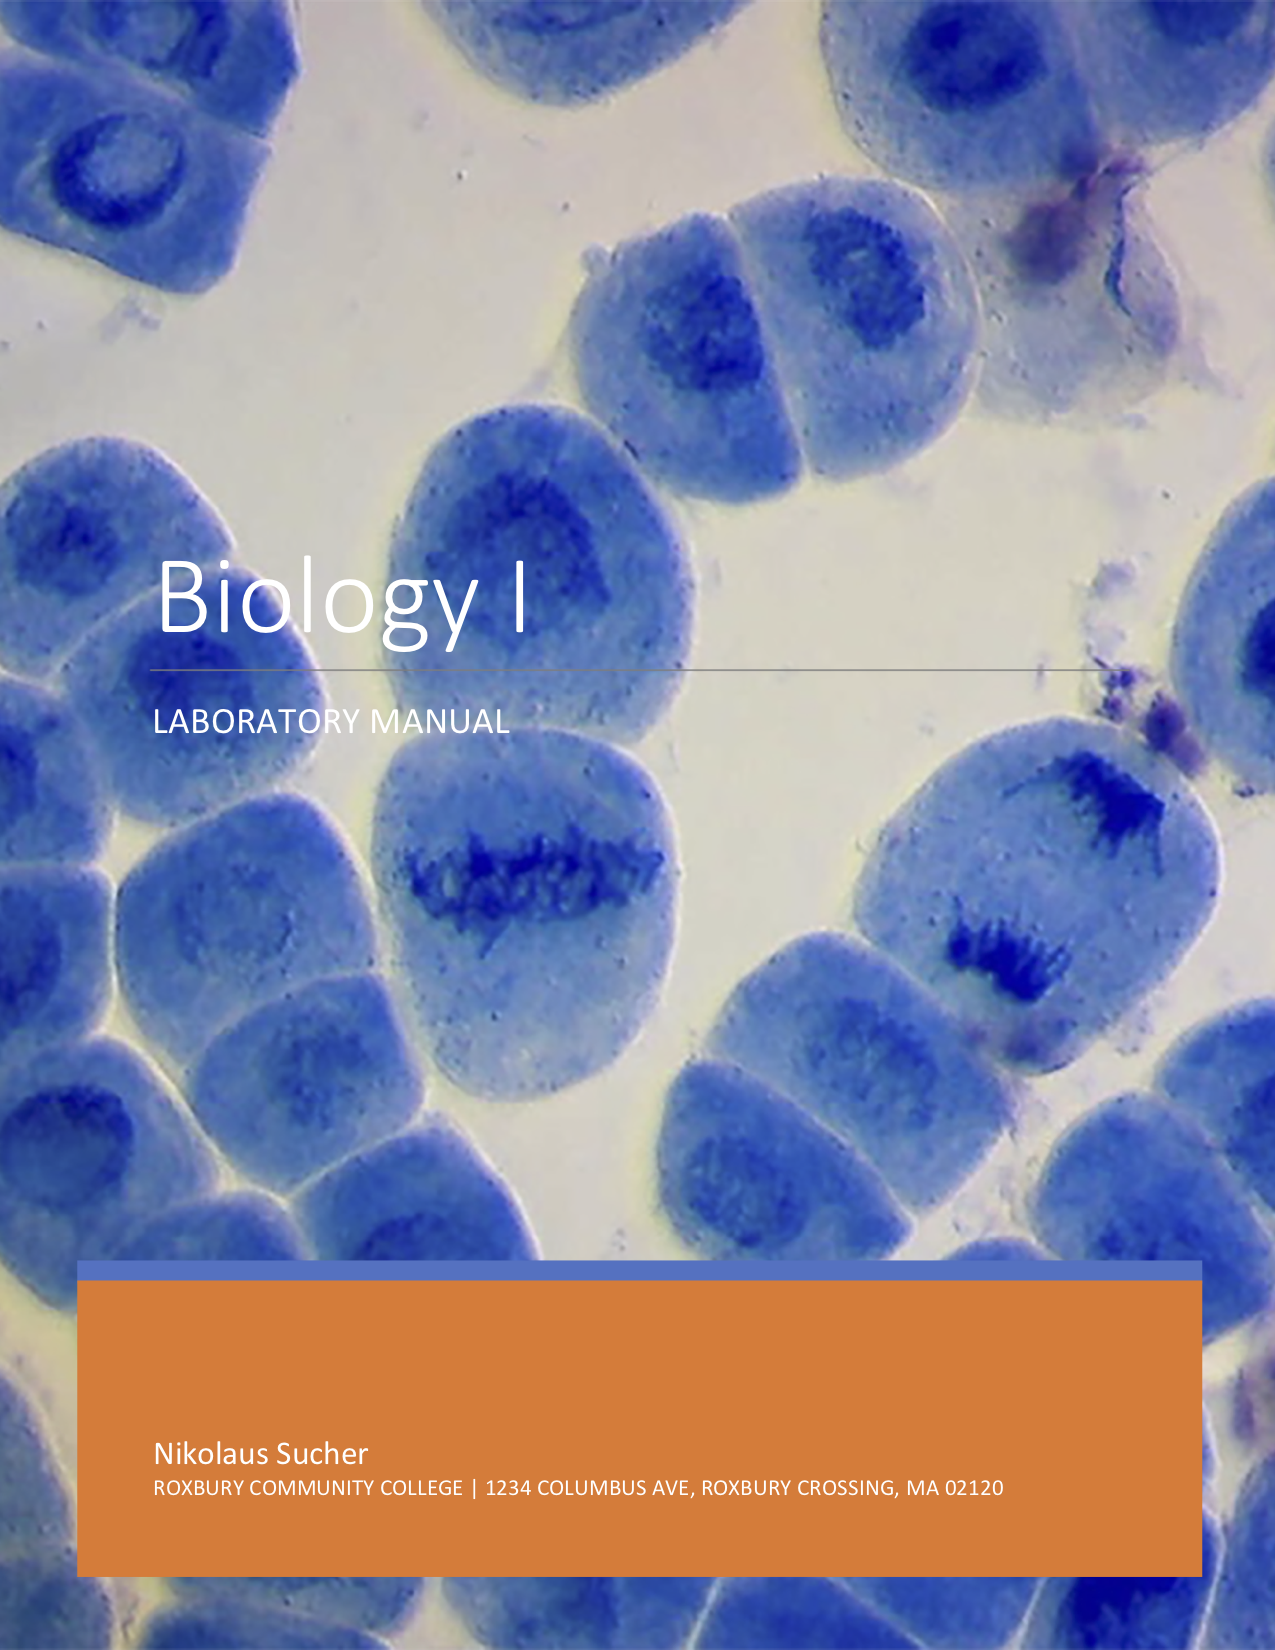
\includegraphics[width=0.7\linewidth]{cover} \end{center}

This work is licensed under the
\href{https://creativecommons.org/licenses/by-sa/3.0/deed.en}{Creative
Commons Attribution-Share Alike 3.0 Unported} United States License.

\chapter*{Acknowledgements}\label{acknowledgements}
\addcontentsline{toc}{chapter}{Acknowledgements}

At \href{http://www.rcc.mass.edu}{RCC}, introductory (general) biology
is split into two courses (SCI103, Biology I, and SCI104, Biology II)
which are taught over two semesters. The two courses were developed in
the 1970s by Prof.~Georgia Whitman essentially representing botany
(Biology I) and zoology (Biology II). Some 20 years ago, Prof.~Kyrsis
Rodriguez who served as the biology course coordinator until her
retirement reduced the botany content and introduced molecular aspects
of biology.

In 2015, the Massachusetts Department of Higher Education with its
\href{http://www.mass.edu/masstransfer/}{MassTransfer Pathways}
initiative prompted a statewide critical evaluation of the structure and
content of foundational courses, such as introductory biology, in order
to make these courses eligible for transfer across the Commonwealth
amongst public higher education institutions. In 2016, we have been
fortunate to receive a large grant from the
\href{http://www.masslifesciences.com}{Massachusetts Life Sciences
Center} to upgrade and modernize our science labs. We have taken this
opportunity to re-structure our courses along the lines of current
practice of introductory biology teaching such that the Biology I course
introduces the molecular and cellular basis of life, while the Biology
II course is focused on the basics of organismal biology. Overall the
proposed changes will expose our students to modernized (up-to-date)
concepts of biology and thus make them more competitive.

This laboratory manual was inspired by
``\href{https://www.amazon.com/Encounters-Life-General-Biology-Laboratory/dp/0895826852}{Encounters
with Life}'' by Larry J. Scott and Hans F. E. Wachtmeister published by
the Morton Publishing Company in Englewood CO. We used that manual at
RCC for many years. Progress in the biological sciences is, however,
relentless and so over the years, our requirements changed, and we felt
that it was best to put together a new manual specifically tailored to
our needs.

The creation of this manual was greatly facilitated and owes a major
debt to Wikipedia and its large number of voluntary contributors. I very
liberally copied from many Wikipedia pages and then remixed, edited,
adapted and added text. With your continued support and help this manual
can only get better over time. I urge you to email me with your
criticisms and suggestions at
\href{mailto:nsucher@rcc.mass.edu}{\nolinkurl{nsucher@rcc.mass.edu}}.
This manual is made available as an open educational resource under
\href{https://creativecommons.org/licenses/by-sa/3.0/deed.en}{Creative
Commons Attribution-Share Alike 3.0 Unported} United States License for
others to do as I did and improve and adapt to specific requirements.

I wish to thank Dr.~Hillel Sims, Dean of STEM, for the laboratory safety
and microscope videos. Thanks to Prof.~Bruce Brender for suggesting the
catalase experiments, which are based on the experiments in the Lab
Manual for Biology by Sylvia Mader published by McGraw-Hill. I wish to
thank Andrea Thomason and Dr.~Maria Carles for the strawberry DNA
extraction protocol. Thanks also go to Daveen Blythe, Director of
Science Laboratories at RCC, for working hard setting up the new
experiments. Last but not least, I want to thank all lab technicians, my
teaching colleagues and our students who work together to translate mere
words into an exciting laboratory experience for all of us at RCC.

\chapter{Course Description}\label{course-description}

This course provides an introduction to the molecular and cellular basis
of life, the theory of evolution and the diversity of microscopic
organisms. Four hours of lecture and a two-hour lab session are required
each week.

\section{Learning Objectives}\label{learning-objectives}

\begin{itemize}
\item
  Identify the basic characteristics of life and outline the theories
  that attempt to explain the origin of life, as we know it and define
  it, on the planet Earth.
\item
  Identify some basic chemical concepts and apply them to the structure
  and biological processes that occur in living cells.
\item
  Identify cell parts, and demonstrate understanding of their related
  functions. Identify similarities and differences in the structure of
  viruses, prokaryotic cells, and eukaryotic cells
\item
  Explain the significance of enzymes, coenzymes, and ATP, and to
  identify the main events, products and significance of the processes
  of cell respiration, fermentation, and photosynthesis
\item
  Understand, explain, and contrast the processes of mitosis, meiosis,
  and binary fission in terms of their physical differences and their
  genetic and evolutionary significance. Explain the process of viral
  replication
\item
  Identify the structural parts of DNA and RNA, and understand how DNA
  directs the activities of a cell through protein synthesis, including
  some examples of how this process is regulated
\item
  Demonstrate understanding of how genes are passed from one generation
  to the next by completing representative genetic problems and
  explaining/applying genetic concepts
\item
  Demonstrate understanding of the three Domains of Life (Archaea,
  Bacteria and Eukarya) and viruses. Identify some of the distinguishing
  characteristics of each domain and the viruses
\item
  Learn and apply the laboratory skills associated with the objectives
  listed above
\item
  Explain the basic concepts of biology in written and oral form
\item
  Apply the concepts learned to better understand the biological world,
  and the problems that affect human society
\end{itemize}

\chapter{How to do well in this
class}\label{how-to-do-well-in-this-class}

\section*{Before the lab}\label{before-the-lab}
\addcontentsline{toc}{section}{Before the lab}

\begin{itemize}
\tightlist
\item
  Know what's coming up. Each week, look at the schedule to know what
  lab is coming up.
\item
  Be prepared. Read the chapter in the manual \textbf{before} you come
  to the lab.
\item
  In your own words, explain to yourself or someone else what the
  upcoming lab is about.
\end{itemize}

\section*{During the lab}\label{during-the-lab}
\addcontentsline{toc}{section}{During the lab}

\begin{itemize}
\tightlist
\item
  Read the lab instructions carefully.
\item
  Follow the instructions carefully.
\item
  Make sure that you know what you are doing and why you are doing it.
\item
  Don't be afraid to ask your instructor for help or clarifications.
\end{itemize}

\section*{After the lab}\label{after-the-lab}
\addcontentsline{toc}{section}{After the lab}

\begin{itemize}
\tightlist
\item
  Ask yourself: what was this lab about? What did we do? How did we do
  it?
\item
  In your own words, tell yourself or someone else what you learned in
  the lab.
\end{itemize}

\chapter{Lab Safety}\label{lab-safety}

The laboratory classes are hands-on. Some classes require the use of
hazardous chemicals and materials. Safety in the classroom is the \#1
priority for students and faculty. To ensure a safe science laboratory,
a list of rules must be followed at all times.

Please watch the \href{https//youtu.be/NxcsyTv7stQ}{RCC safety video}

\BeginKnitrBlock{rmdimportant}
\textbf{Prior to your participation in the science lab course, you must
read this safety document and sign and return the acknowledgment and
agreement page.}
\EndKnitrBlock{rmdimportant}

\section{General rules}\label{general-rules}

\begin{enumerate}
\def\labelenumi{\arabic{enumi}.}
\tightlist
\item
  NO FOOD, BEVERAGES, GUM, in the labs. Cell phone usage is also
  prohibited in the lab.
\item
  Conduct yourself in a responsible manner at all times in the lab.
  Horseplay, pranks and practical jokes are prohibited and will not be
  tolerated. If you participate in inappropriate behavior the INSTRUCTOR
  HAS THE RIGHT TO ASK YOU TO LEAVE THE lab.
\item
  Students cannot be in the lab without an instructor present.
\item
  Read all lab procedures, precautions, and equipment instructions
  thoroughly before each lab. Follow all written and verbal instructions
  carefully. Perform only those experiments authorized by the
  instructor. If during the lab you don't understand, stop and ask the
  instructor before proceeding. Never do anything in the lab that is
  outside of your instructors directions or that is not in your lab
  procedure.
\item
  Do not begin lab activities; touch any chemicals or equipment until
  you are instructed to do so.
\item
  Work areas should be kept organized and clean at all times. Only
  necessary items (lab notebook, worksheets, etc.) should be on your
  workbench. Backpacks and purses must be stored under the benches or
  against the walls. CLEAN ALL OF YOUR WORK SURFACES AND EQUIPMENT AT
  THE END OF THE EXPERIMENT. Safely dispose of waste in its proper
  container and place glassware in the grey bins by the sink. DO NOT
  STACK GLASSWARE. If the bin is full ask the instructor for another
  bin.
\item
  Keep aisles clear. Push lab stools under the lab benches when not in
  use.
\item
  Know where the safety equipment is and how to use it. This includes
  the first aid kit, eyewash station, safety shower, fire extinguisher,
  and fire blanket. Know the location of the fire alarm, and emergency
  phone. In the event of a fire drill during lab time containers must be
  closed, gas valves off, fume hood, and all electrical equipment must
  be turned off.
\item
  NEVER DISPOSE OF ANYTHING IN THE SINK. All materials are to be
  disposed of in the proper hazardous waste containers with the
  assistance of the instructor. All waste containers must be closed and
  placed inside a secondary containment bin.
\item
  As classes in these labs use toxic chemicals, keep your hands away
  from your face, eyes and mouth while working in the lab. Always wash
  your hands thoroughly with warm water and soap before leaving the lab
  to prevent injury or illness. This is part of proper lab procedure.
\item
  Students are not permitted in the prep room areas (between the lab
  rooms).
\item
  Handle all living organisms used for lab experiments in a respectful,
  humane manner.
\item
  Microscopes must be properly cleaned, the electrical cords properly
  wrapped, and returned to their places with their protective covers.
\end{enumerate}

Disposal of all hazardous waste is ONLY to be handled by the instructor
and in a manner consistent with federal, state and local hazardous waste
disposal regulations. Organic solvents are never to be disposed of down
the sink; receptacles will be provided as needed for their collection.
All hazardous chemical substances must be placed in the appropriate type
of container and labeled with chemical, name and date, sealed and placed
upright in a gray plastic bin.

\section{Class dissections}\label{class-dissections}

\begin{enumerate}
\def\labelenumi{\arabic{enumi}.}
\setcounter{enumi}{13}
\tightlist
\item
  Preserved biological specimens should be treated with respect and
  disposed of in a clear plastic bag and placed inside the hazardous
  waste drum located in the classroom. This container must be sealed at
  the end of each dissection.
\item
  When using sharp objects always carry the tips pointed down and away
  from you. When dissecting, cut away from your body. Grasp the
  instrument only by the handle. Never try to catch falling sharp
  instruments or glassware. When you are finished dissecting, wash and
  dry your instruments and dissecting pan before storing them in the
  proper location. Do not leave any instruments in the sink.
\end{enumerate}

\section{Clothing}\label{clothing}

\begin{enumerate}
\def\labelenumi{\arabic{enumi}.}
\setcounter{enumi}{15}
\tightlist
\item
  Students must wear lab goggles when using chemicals, or using heat. NO
  EXCEPTIONS! Lab coats are mandatory for Anatomy and Physiology,
  Biology, Microbiology, Chemistry, and Biotechnology labs, except for
  when lecturing and working on dry lab (for example, looking at models
  or prepared slides) activities.
\item
  Gloves should be worn when handling solutions, solids, specimens, etc.
\item
  Proper dress should always be observed in the lab. Long hair must be
  tied back. Loose or baggy clothing (especially sleeves), dangling
  jewelry, hats, shorts, short skirts, bare mid riffs, high heels,
  sleeveless shirts, and open toed or open heeled shoes and sandals are
  prohibited in the lab. Failure to comply may result in expulsion from
  class.
\end{enumerate}

\section{Handling chemicals}\label{handling-chemicals}

\begin{enumerate}
\def\labelenumi{\arabic{enumi}.}
\setcounter{enumi}{17}
\tightlist
\item
  Always work in a well-ventilated area. Use the fume hood when working
  with volatile substances or poisonous vapors, or any chemical with an
  odor.
\item
  Never smell a chemical by sniffing. Use your hand to wave the chemical
  towards your nose.
\item
  DO NOT TASTE, TOUCH or smell anything unless instructed to do so. You
  should wear a lab apron and gloves at all times. Your instructor will
  tell you the proper gloves to wear depending on the chemical being
  used.
\item
  CHECK EACH LABEL TWICE before removing any of its contents. Take only
  what is needed of each chemical. NEVER return unused chemicals to
  their original container; put it in the waste container.
\item
  Do not use your fingers to transfer solid chemicals. Use a scoop or
  spatula.
\item
  Use a rubber bulb, pipette, or pi-pump when transferring liquid
  chemicals. NEVER USE YOUR MOUTH TO PIPETTE!
\item
  When transferring reagents hold the containers away from your body
  while working on the bench.
\item
  Acids must be handled with extreme care. You will be shown the proper
  method for diluting strong acids. ALWAYS ADD ACID TO WATER, swirl or
  invert the solution and be careful of the heat produced particularly
  with sulfuric acid.
\item
  Handle hazardous liquids over a pan to contain spills.
\item
  Never handle flammable liquids anywhere near an open flame or heat
  source.
\item
  Be careful when transporting chemicals across the lab. Hold securely
  and walk carefully.
\item
  NEVER POUR CHEMICALS INTO SINK. Waste should be disposed of in the
  proper hazardous waste container provided.
\end{enumerate}

\section{Glassware}\label{glassware}

\begin{enumerate}
\def\labelenumi{\arabic{enumi}.}
\setcounter{enumi}{29}
\tightlist
\item
  Never handle broken glass with bare hands. Use a brush and a dustpan
  to clean up broken glass. Place uncontaminated broken glass in the
  white and blue broken glass receptacles. Contaminated trash goes in
  the biohazard bin.
\item
  Fill wash bottles only with distilled water and use only as intended,
  e.g.; rinsing glassware, adding water to a container.
\item
  Never use chipped, cracked or dirty glassware to avoid shattering.
\item
  Never immerse hot glassware in cold water. It may shatter.
\item
  Never place dirty glassware with the clean glassware. All dirty
  glassware should be placed in gray wash bins. DO NOT STACK DIRTY
  GLASSWARE IN BINS.
\end{enumerate}

\section{Heating substances}\label{heating-substances}

\begin{enumerate}
\def\labelenumi{\arabic{enumi}.}
\setcounter{enumi}{34}
\tightlist
\item
  Exercise extreme caution when using a gas burner. Be careful to keep
  hair, loose clothing and hands away from flames at all times. Wear
  safety goggles. Do not put any substances into the flame unless
  specifically instructed to do so. Never reach over an exposed flame.
  The instructor will provide a demonstration of the proper way to
  operate a Bunsen burner. Never leave a lighted burner or hot plate
  unattended. Always turn the burner or hot plate off when not in use.
\item
  Do not point the open end of a test tube being heated at yourself or
  anyone else. Never look into a container that's being heated.
\item
  Heated metals and glass remain hot for a very long time. They should
  be set aside to cool and picked up with caution. Use tongs or heat
  protective gloves.
\end{enumerate}

\section{Handling microbiology
materials}\label{handling-microbiology-materials}

\begin{enumerate}
\def\labelenumi{\arabic{enumi}.}
\setcounter{enumi}{37}
\tightlist
\item
  Please be aware that micro labs include work with pathogenic
  organisms. Be alert. Conduct yourself in a responsible manner at all
  times.
\item
  If you spill anything notify your instructor immediately. There are
  special procedures to be followed for spills containing
  microorganisms.
\item
  A lab coat must be worn during lab activities. Lab coats/aprons may
  never leave the lab. If you must leave the lab during a class then
  your lab coat must be removed.
\item
  Gloves must be worn at all times when working with bacteria. Gloves
  need to be disposed of in the biohazard waste container.
\item
  All contaminated waste must be disposed of in the biohazard container.
  Do not overfill biohazard containers.
\item
  You must spray down your lab bench with Lysol after each lab. Do not
  wipe with paper towels. The bench surface must remain wet for at least
  five minutes for the Lysol to destroy any micro organisms.
\item
  Wash your hands thoroughly before and after each lab as well as before
  you leave the lab for any reason.
\item
  Dispose of contaminated broken glass in the biohazard bin. Please wrap
  the broken glass in paper towels before disposal so that the broken
  glass doesn't cut through the bag. Dispose of uncontaminated glass in
  the white and blue cardboard glass boxes.
\end{enumerate}

\chapter{The Microscope}\label{the-microscope}

A \href{https://en.wikipedia.org/wiki/Microscope}{microscope} (from the
Ancient Greek: mikrós, ``small'' and skopeîn, ``to look'' or ``see'') is
an instrument used to see objects that are too small to be seen by the
naked eye. Microscopic means invisible to the eye unless aided by a
microscope.

There are many types of microscopes, and they may be grouped in
different ways. One way is to describe the way the instruments interact
with a sample to create images, either by sending a beam of light or
electrons to a sample in its optical path, or by scanning across, and a
short distance from, the surface of a sample using a probe. The most
common microscope (and the first to be invented) is the
\href{https://en.wikipedia.org/wiki/Optical_microscope}{optical
microscope}, which uses light to pass through a sample to produce an
image.

The objective lens of a microscope (Figure \ref{fig:objectives}) is a
cylinder containing one or more lenses that are typically made of glass.
It is essentially a high-powered magnifying glass which is brought very
close to the specimen being examined. The objective collects light from
the sample so that it comes to a focus inside the microscope tube. This
creates an enlarged image of the specimen.

\begin{figure}

{\centering 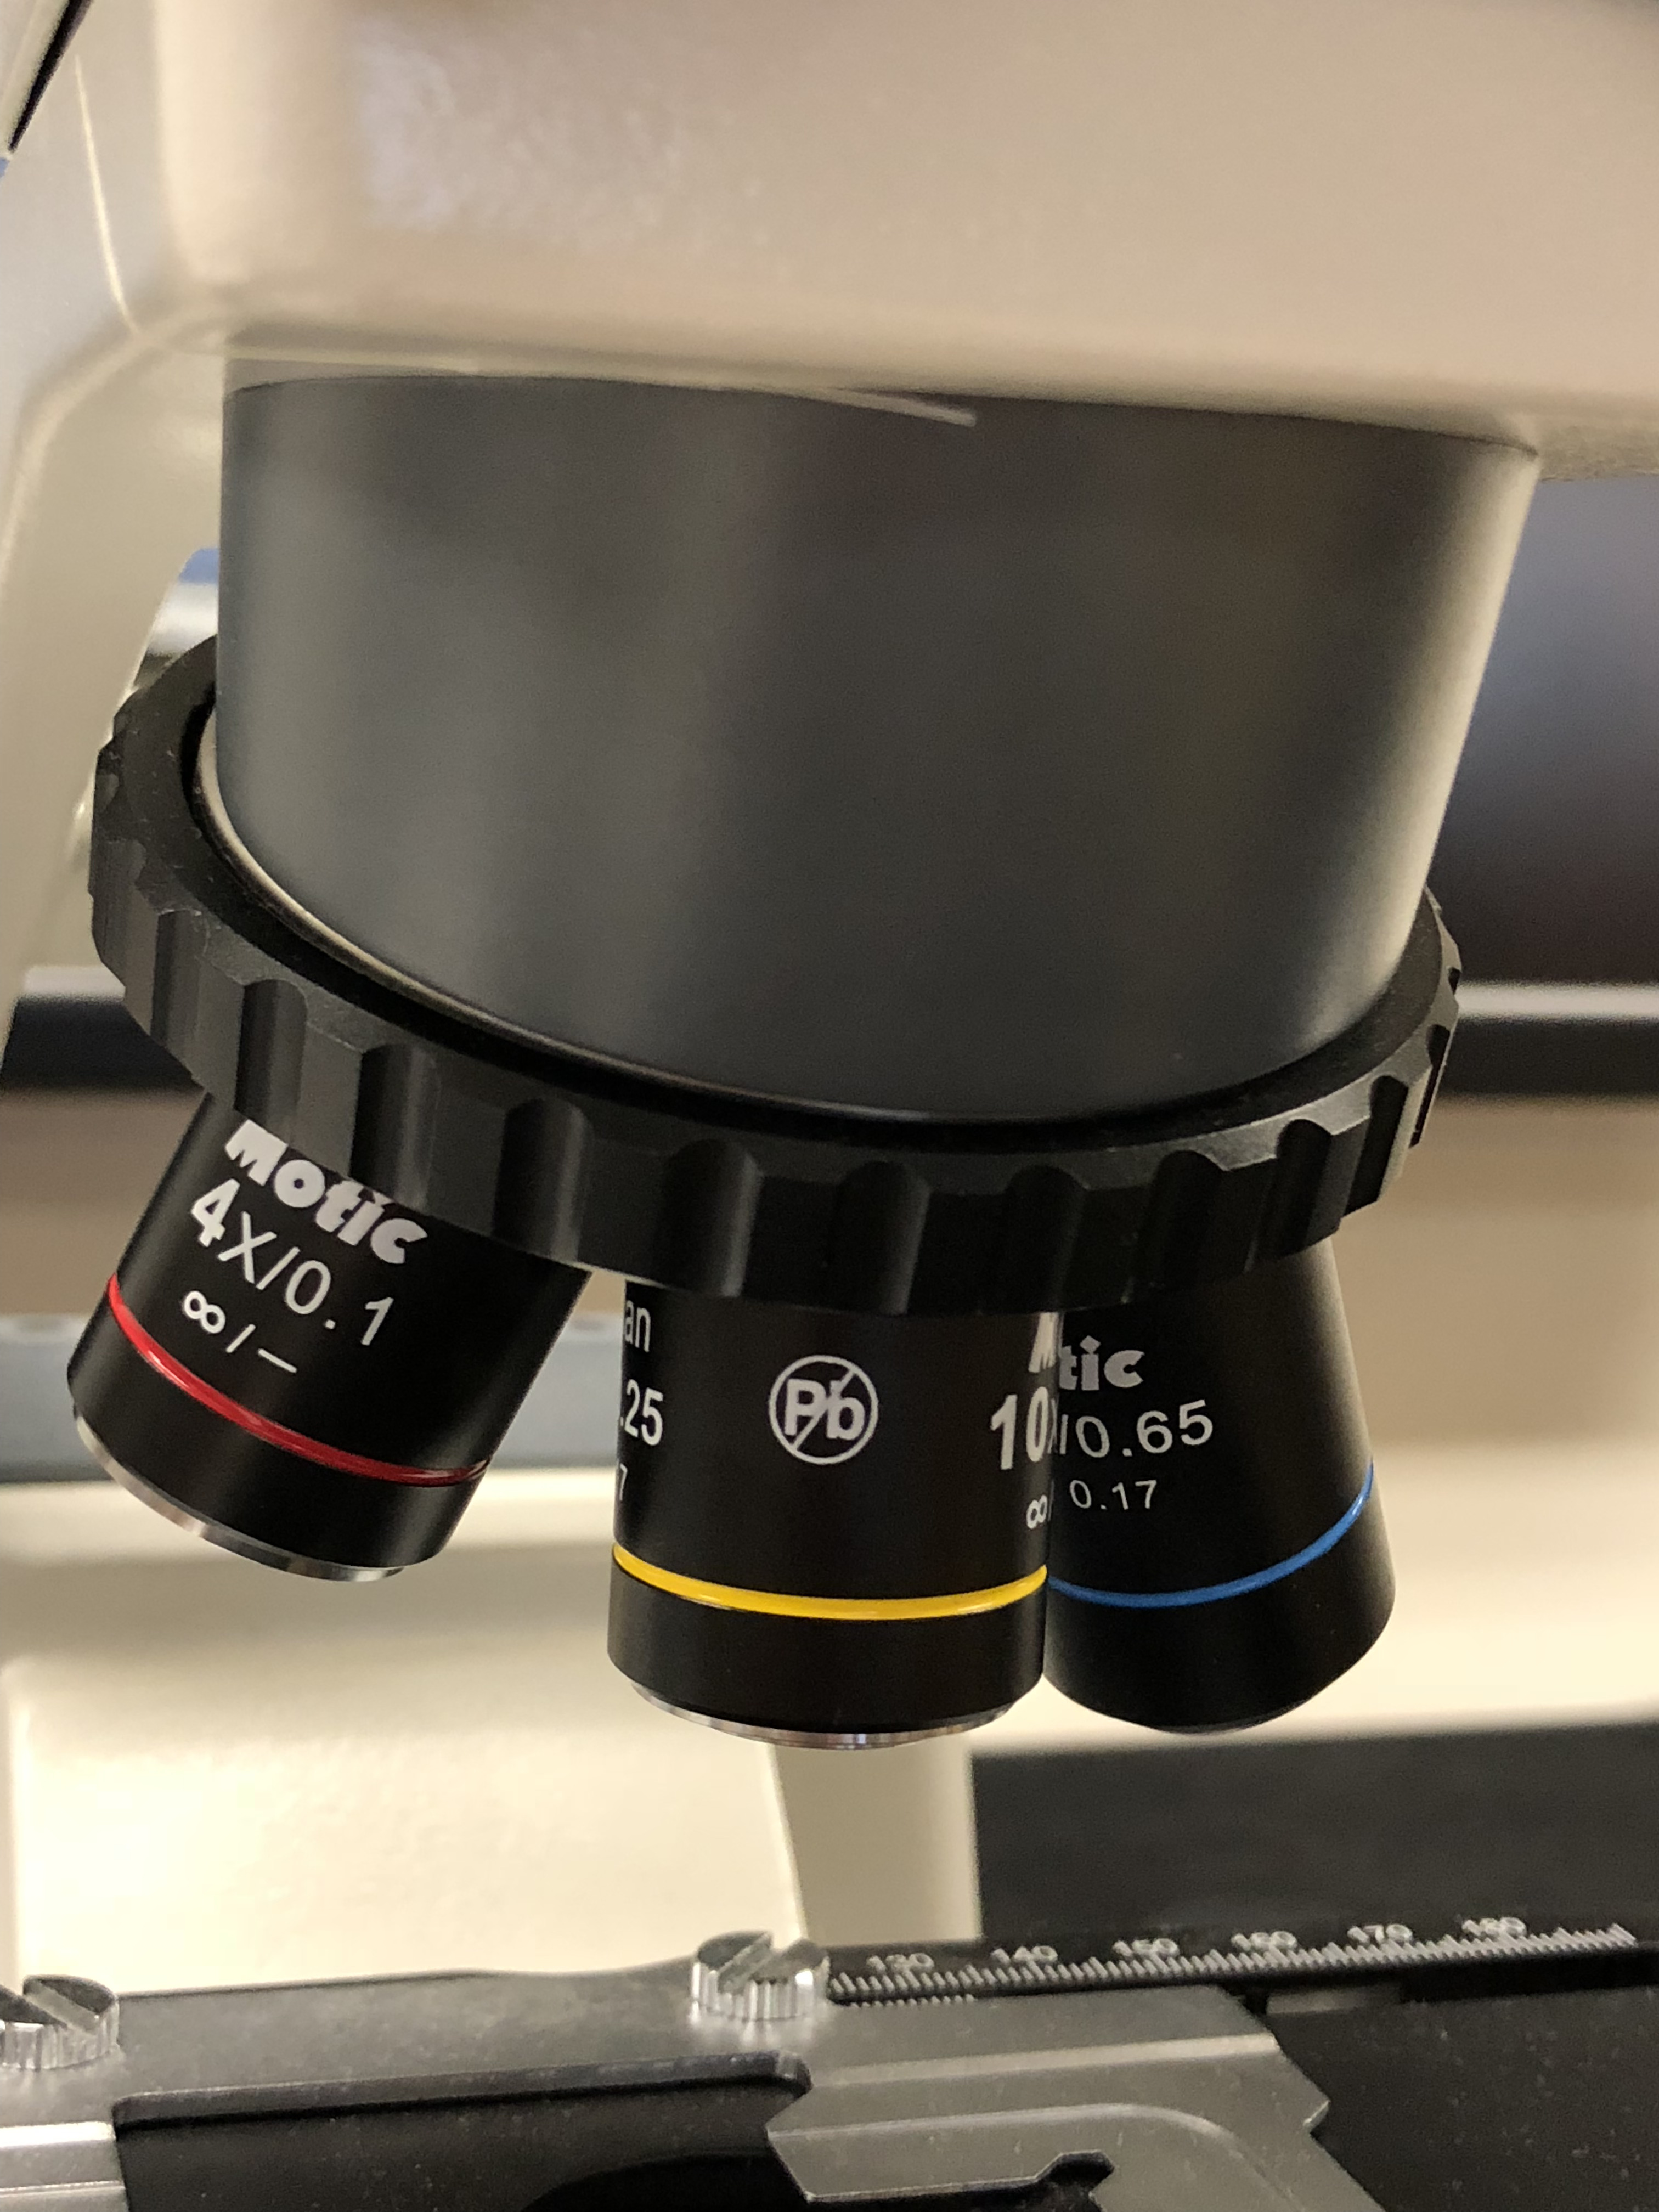
\includegraphics[width=0.7\linewidth]{./figures/microscope/Microscope_objectives} 

}

\caption{The microscope objectives.}\label{fig:objectives}
\end{figure}

The eyepieces, or ocular lenses (Figure \ref{fig:oculars}), are the
lenses that are closest to your eyes when you look through the
microscope. The objective lens or mirror collects light and brings it to
focus creating an image. The eyepiece is placed near the focal point of
the objective to magnify this image. This image is inverted and can be
seen by removing the eyepiece and placing a piece of tracing paper over
the end of the tube. By carefully focusing a brightly lit specimen, a
highly enlarged image can be seen. It is this real image that is viewed
by the eyepiece lens that provides further enlargement. The amount of
magnification depends on the focal length of the eyepiece. The ocular in
our microscopes have a 10× magnification.

\begin{figure}

{\centering 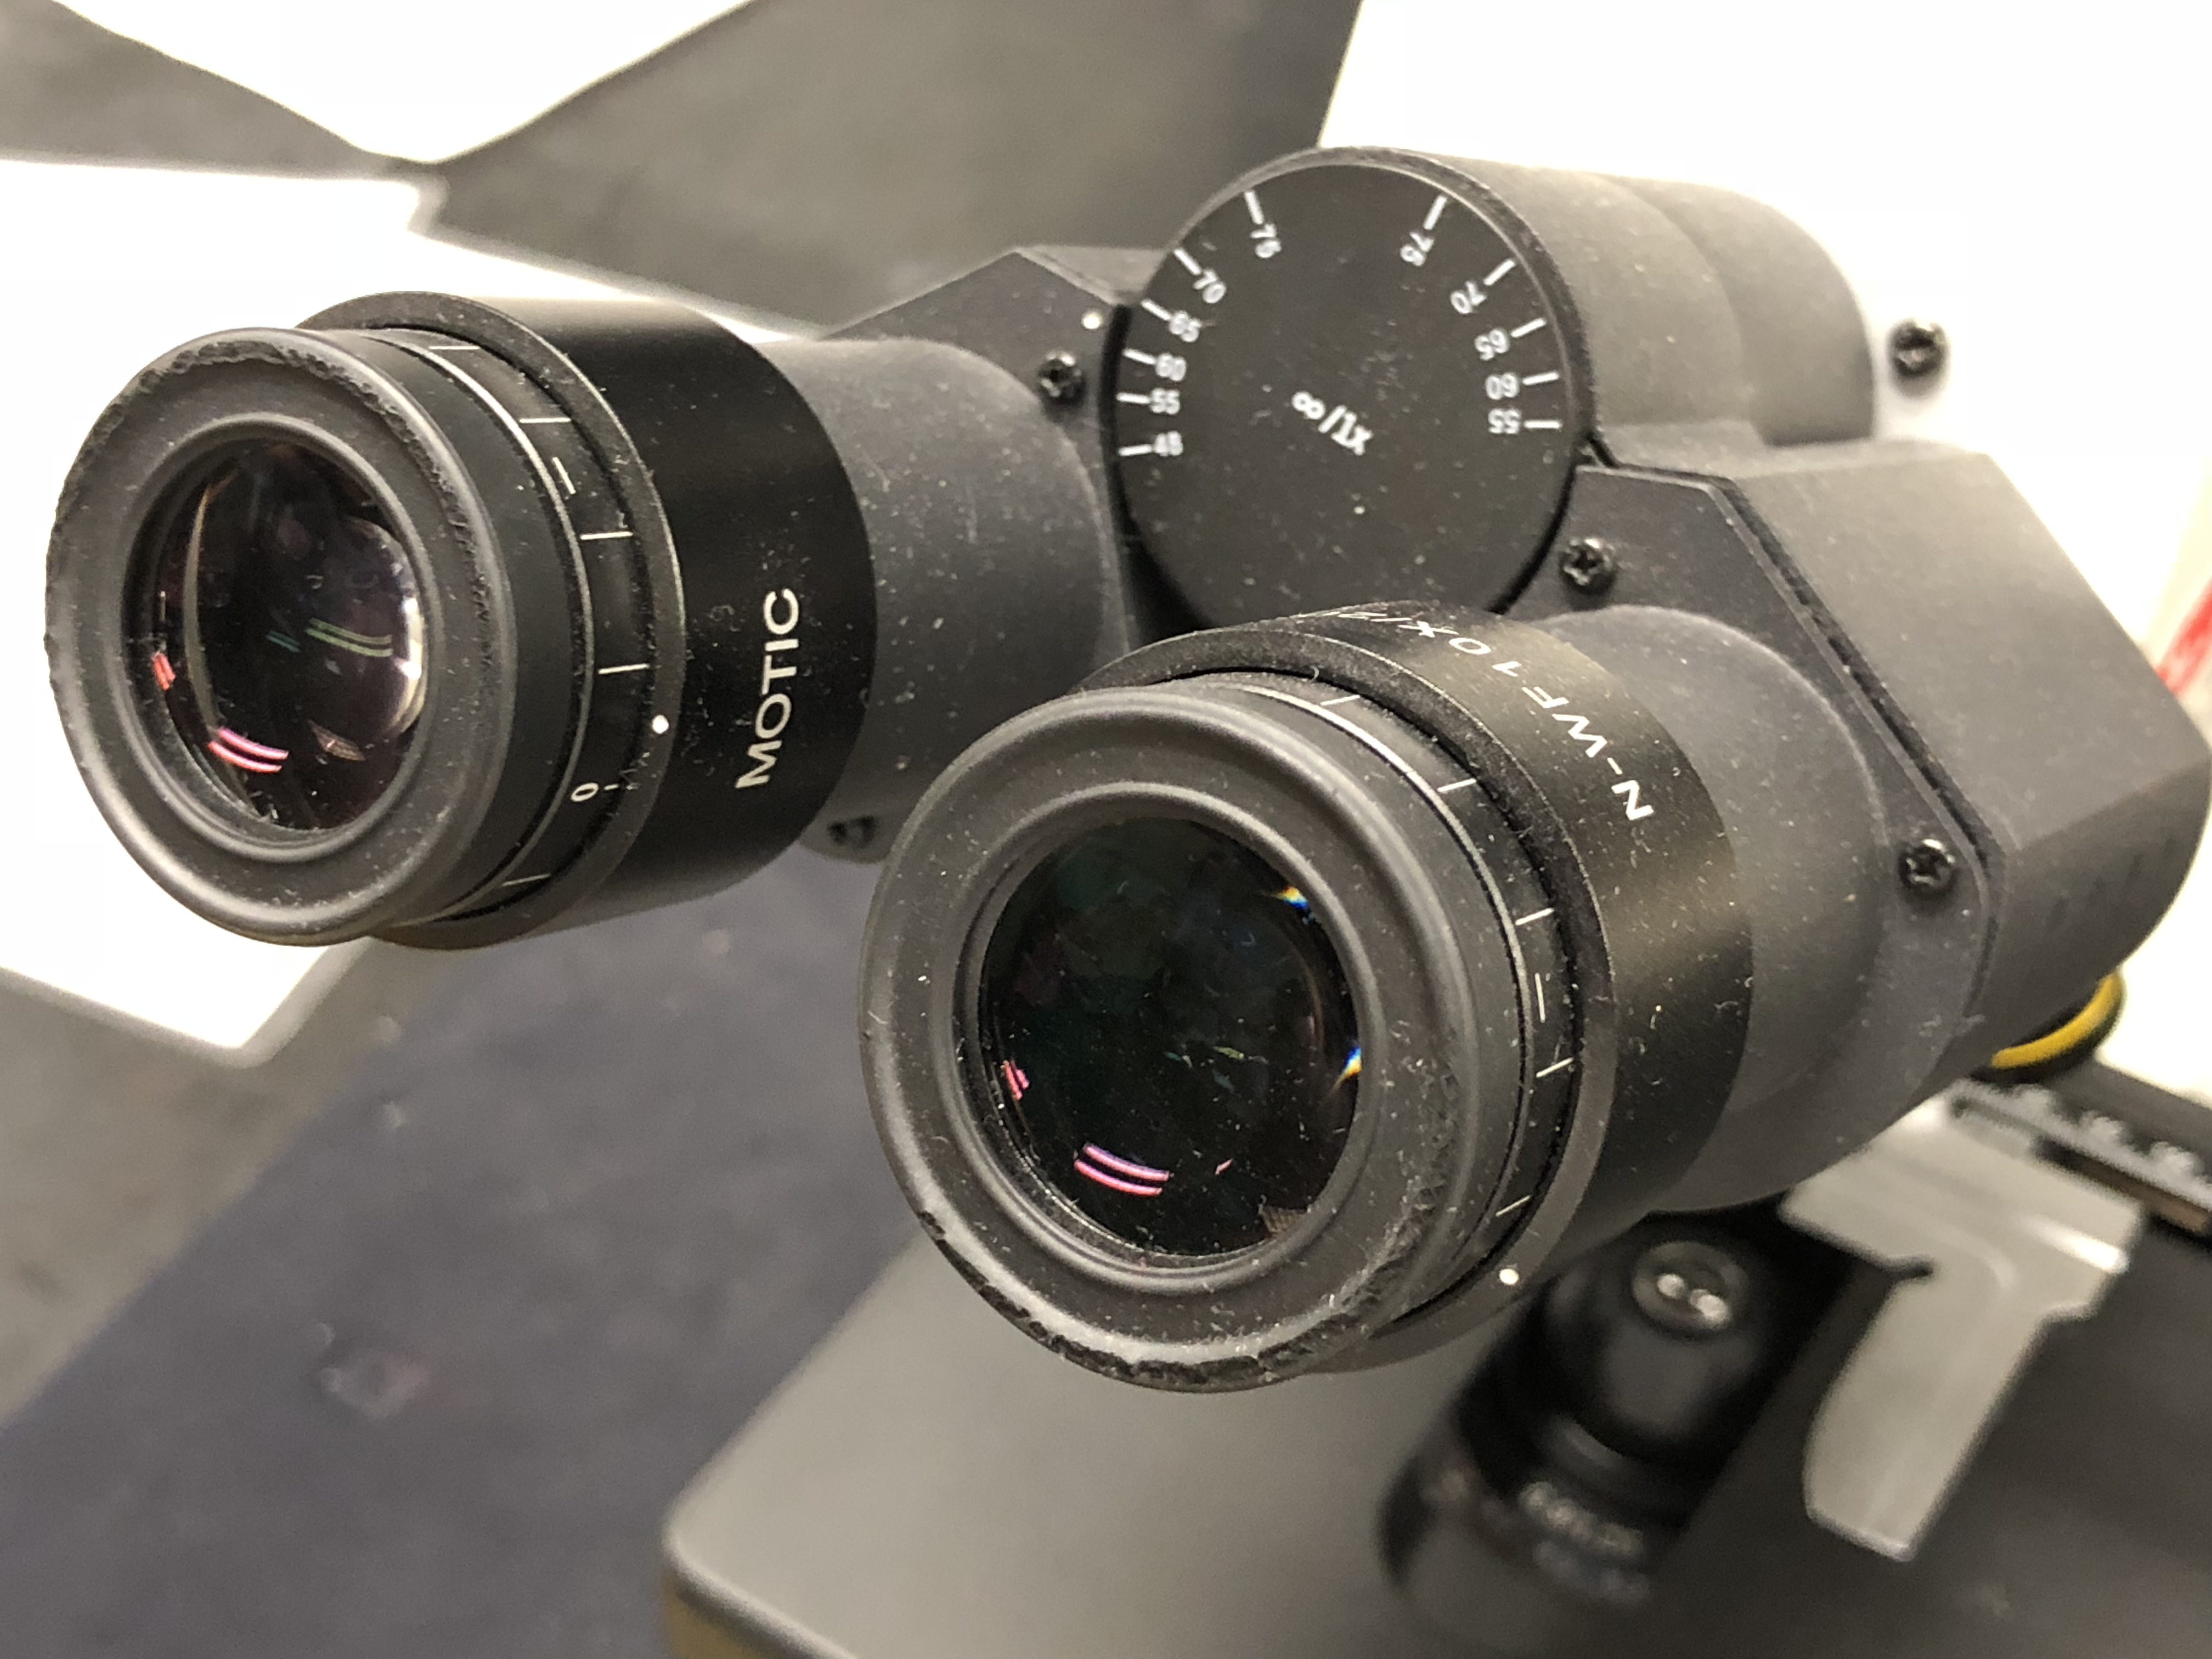
\includegraphics[width=0.7\linewidth]{./figures/microscope/Oculars} 

}

\caption{The oculars (eye pieces) of the microscope.}\label{fig:oculars}
\end{figure}

Our microscopes have four objective lenses with different
magnifications, screwed into the circular ``nosepiece'' which you rotate
to select the required lens. These lenses are color coded for easier
use. The least powerful lens is called the scanning objective lens and
is a 4× objective. The second lens is referred to as the small objective
lens and is 10× lens. The most powerful lens out of the four are
referred to as the large objective lenses and are 40× and 100×. The 100×
objective is an oil-immersion lens. This objective is specially designed
for use with refractive index matching oil, which must fill the gap
between the objective lens and the specimen.

\begin{figure}

{\centering 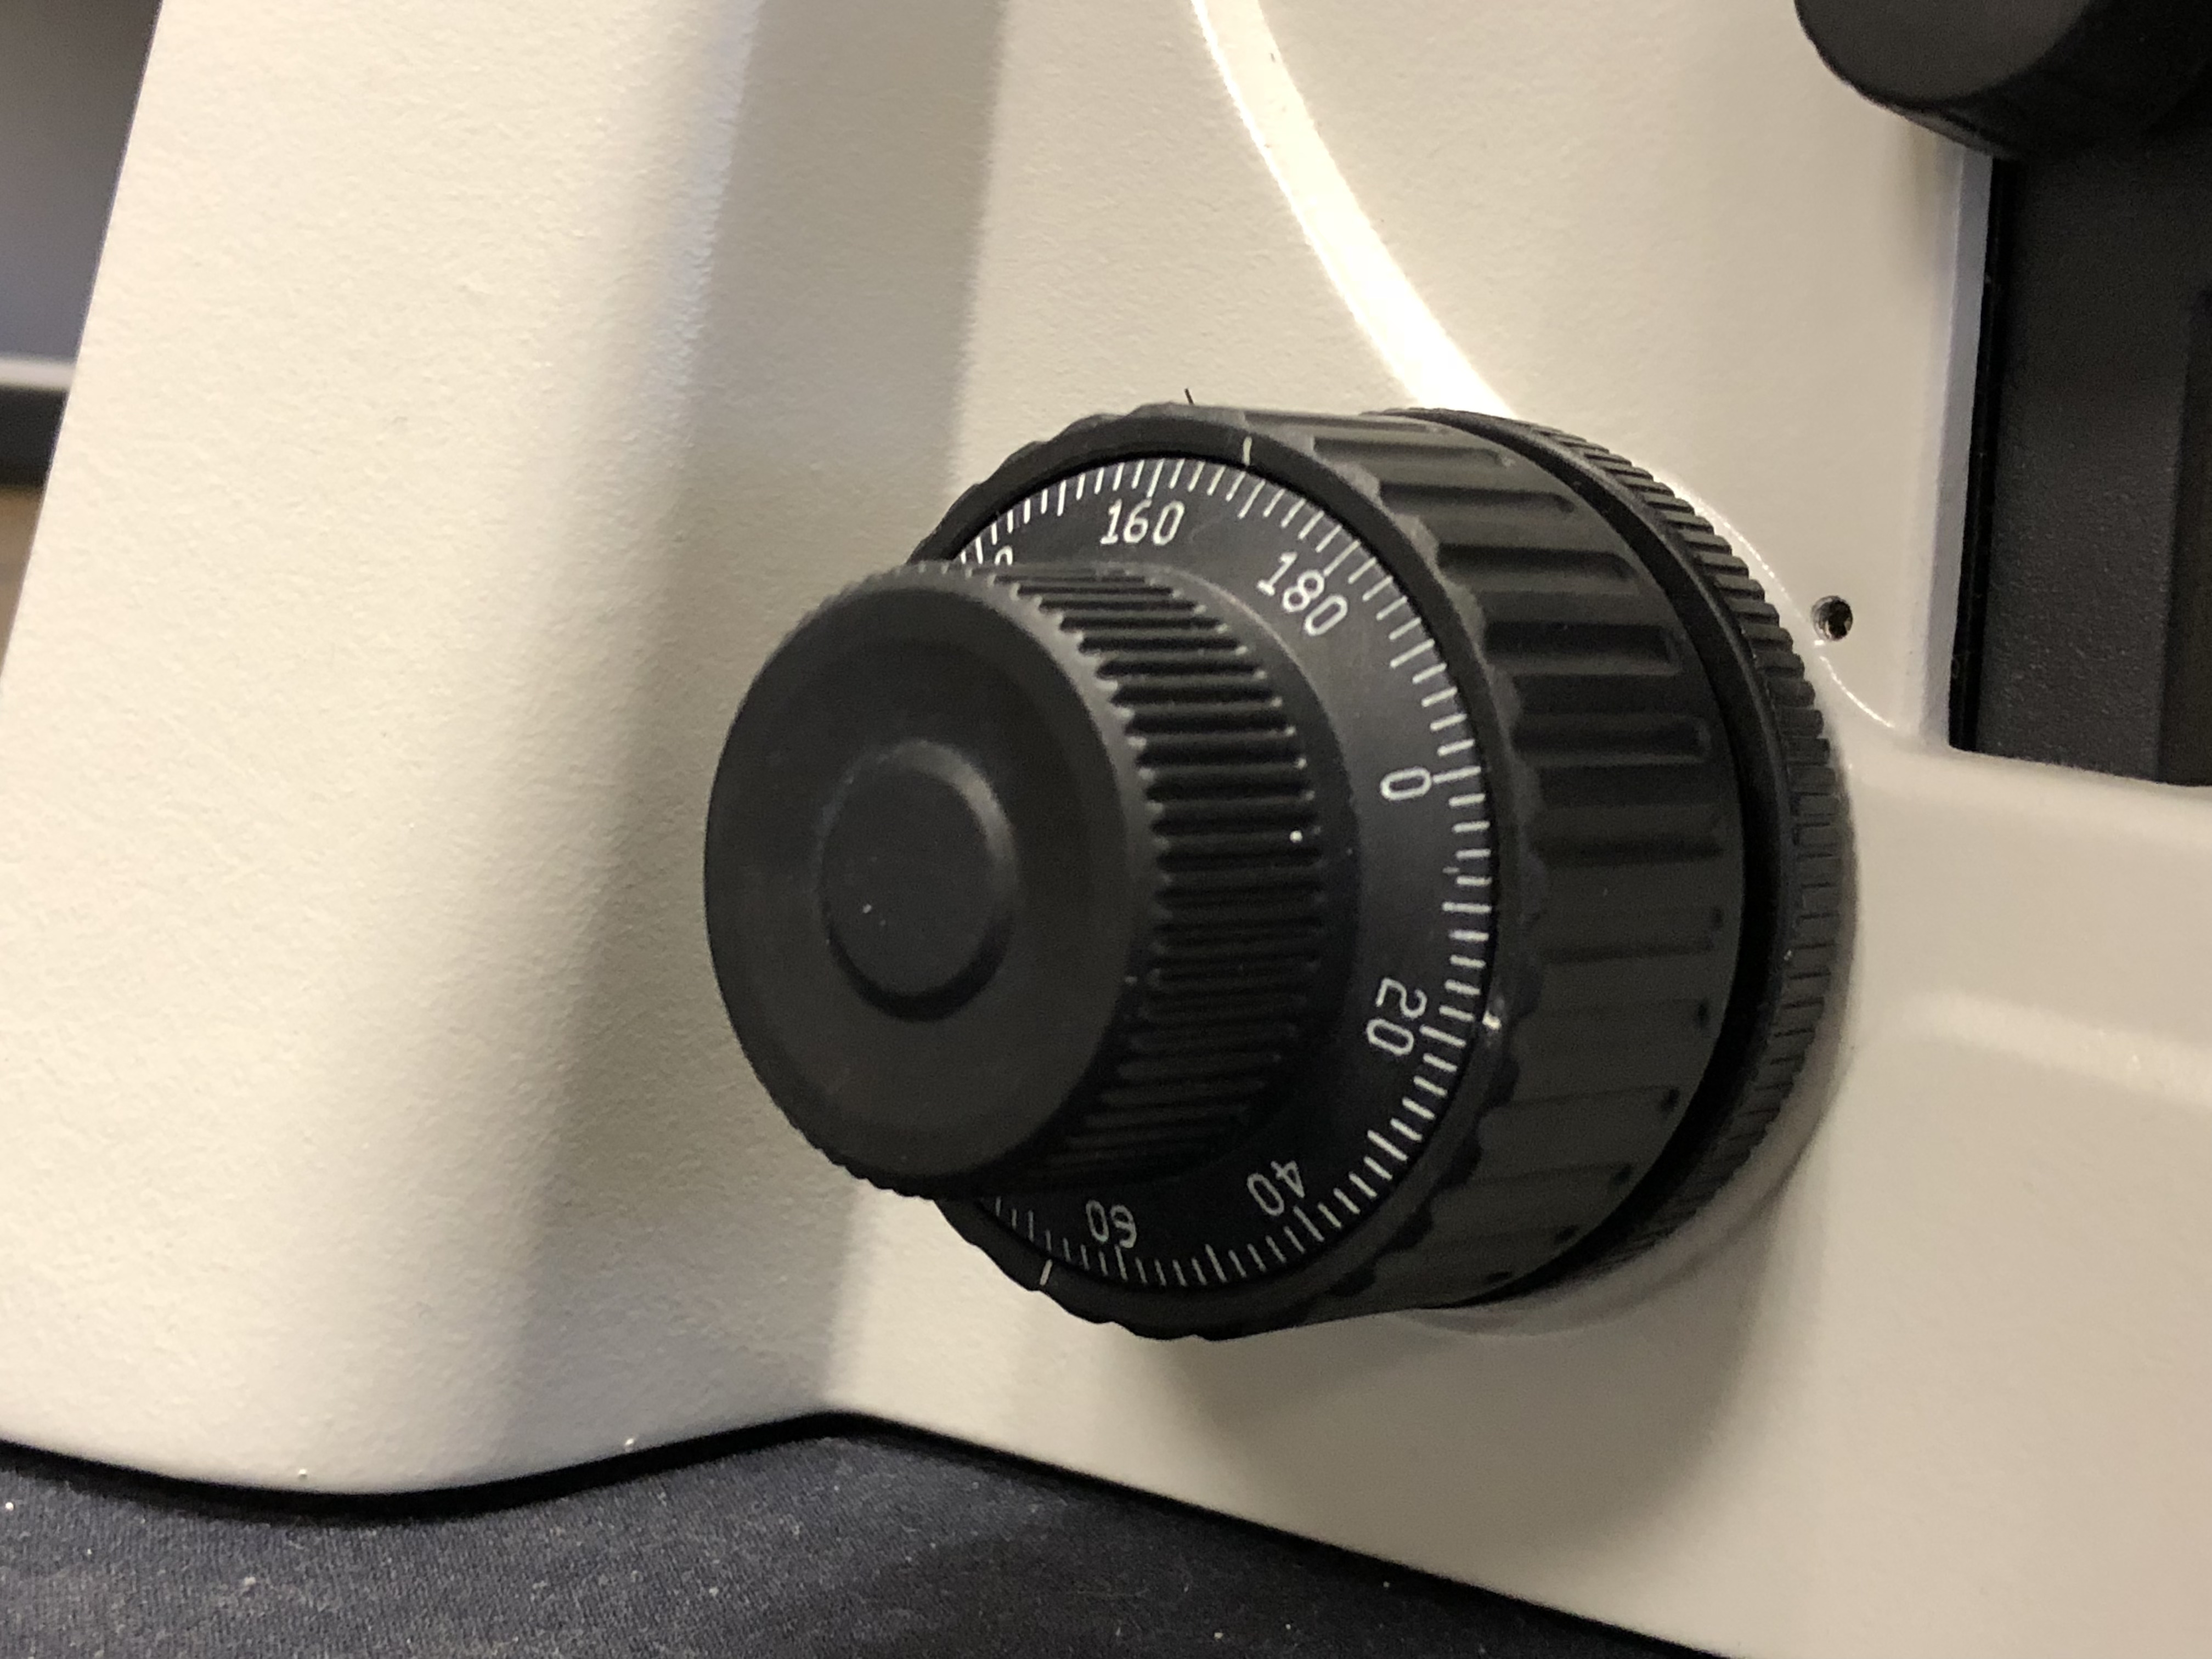
\includegraphics[width=0.7\linewidth]{./figures/microscope/focus} 

}

\caption{The coarse (big wheel) and fine (small wheel) focus adjustment knobs.}\label{fig:focus}
\end{figure}

The stage is a platform below the objective which supports the specimen
being viewed. Adjustment knobs (on the left side of the microscope) move
the stage up and down with separate adjustment for coarse and fine
focusing (Figure \ref{fig:focus}). In the center of the stage is a hole
through which light passes to illuminate the specimen (Figure
\ref{fig:stage}). The stage has arms to hold slides (rectangular glass
plates on which the specimen is mounted).

\begin{figure}

{\centering 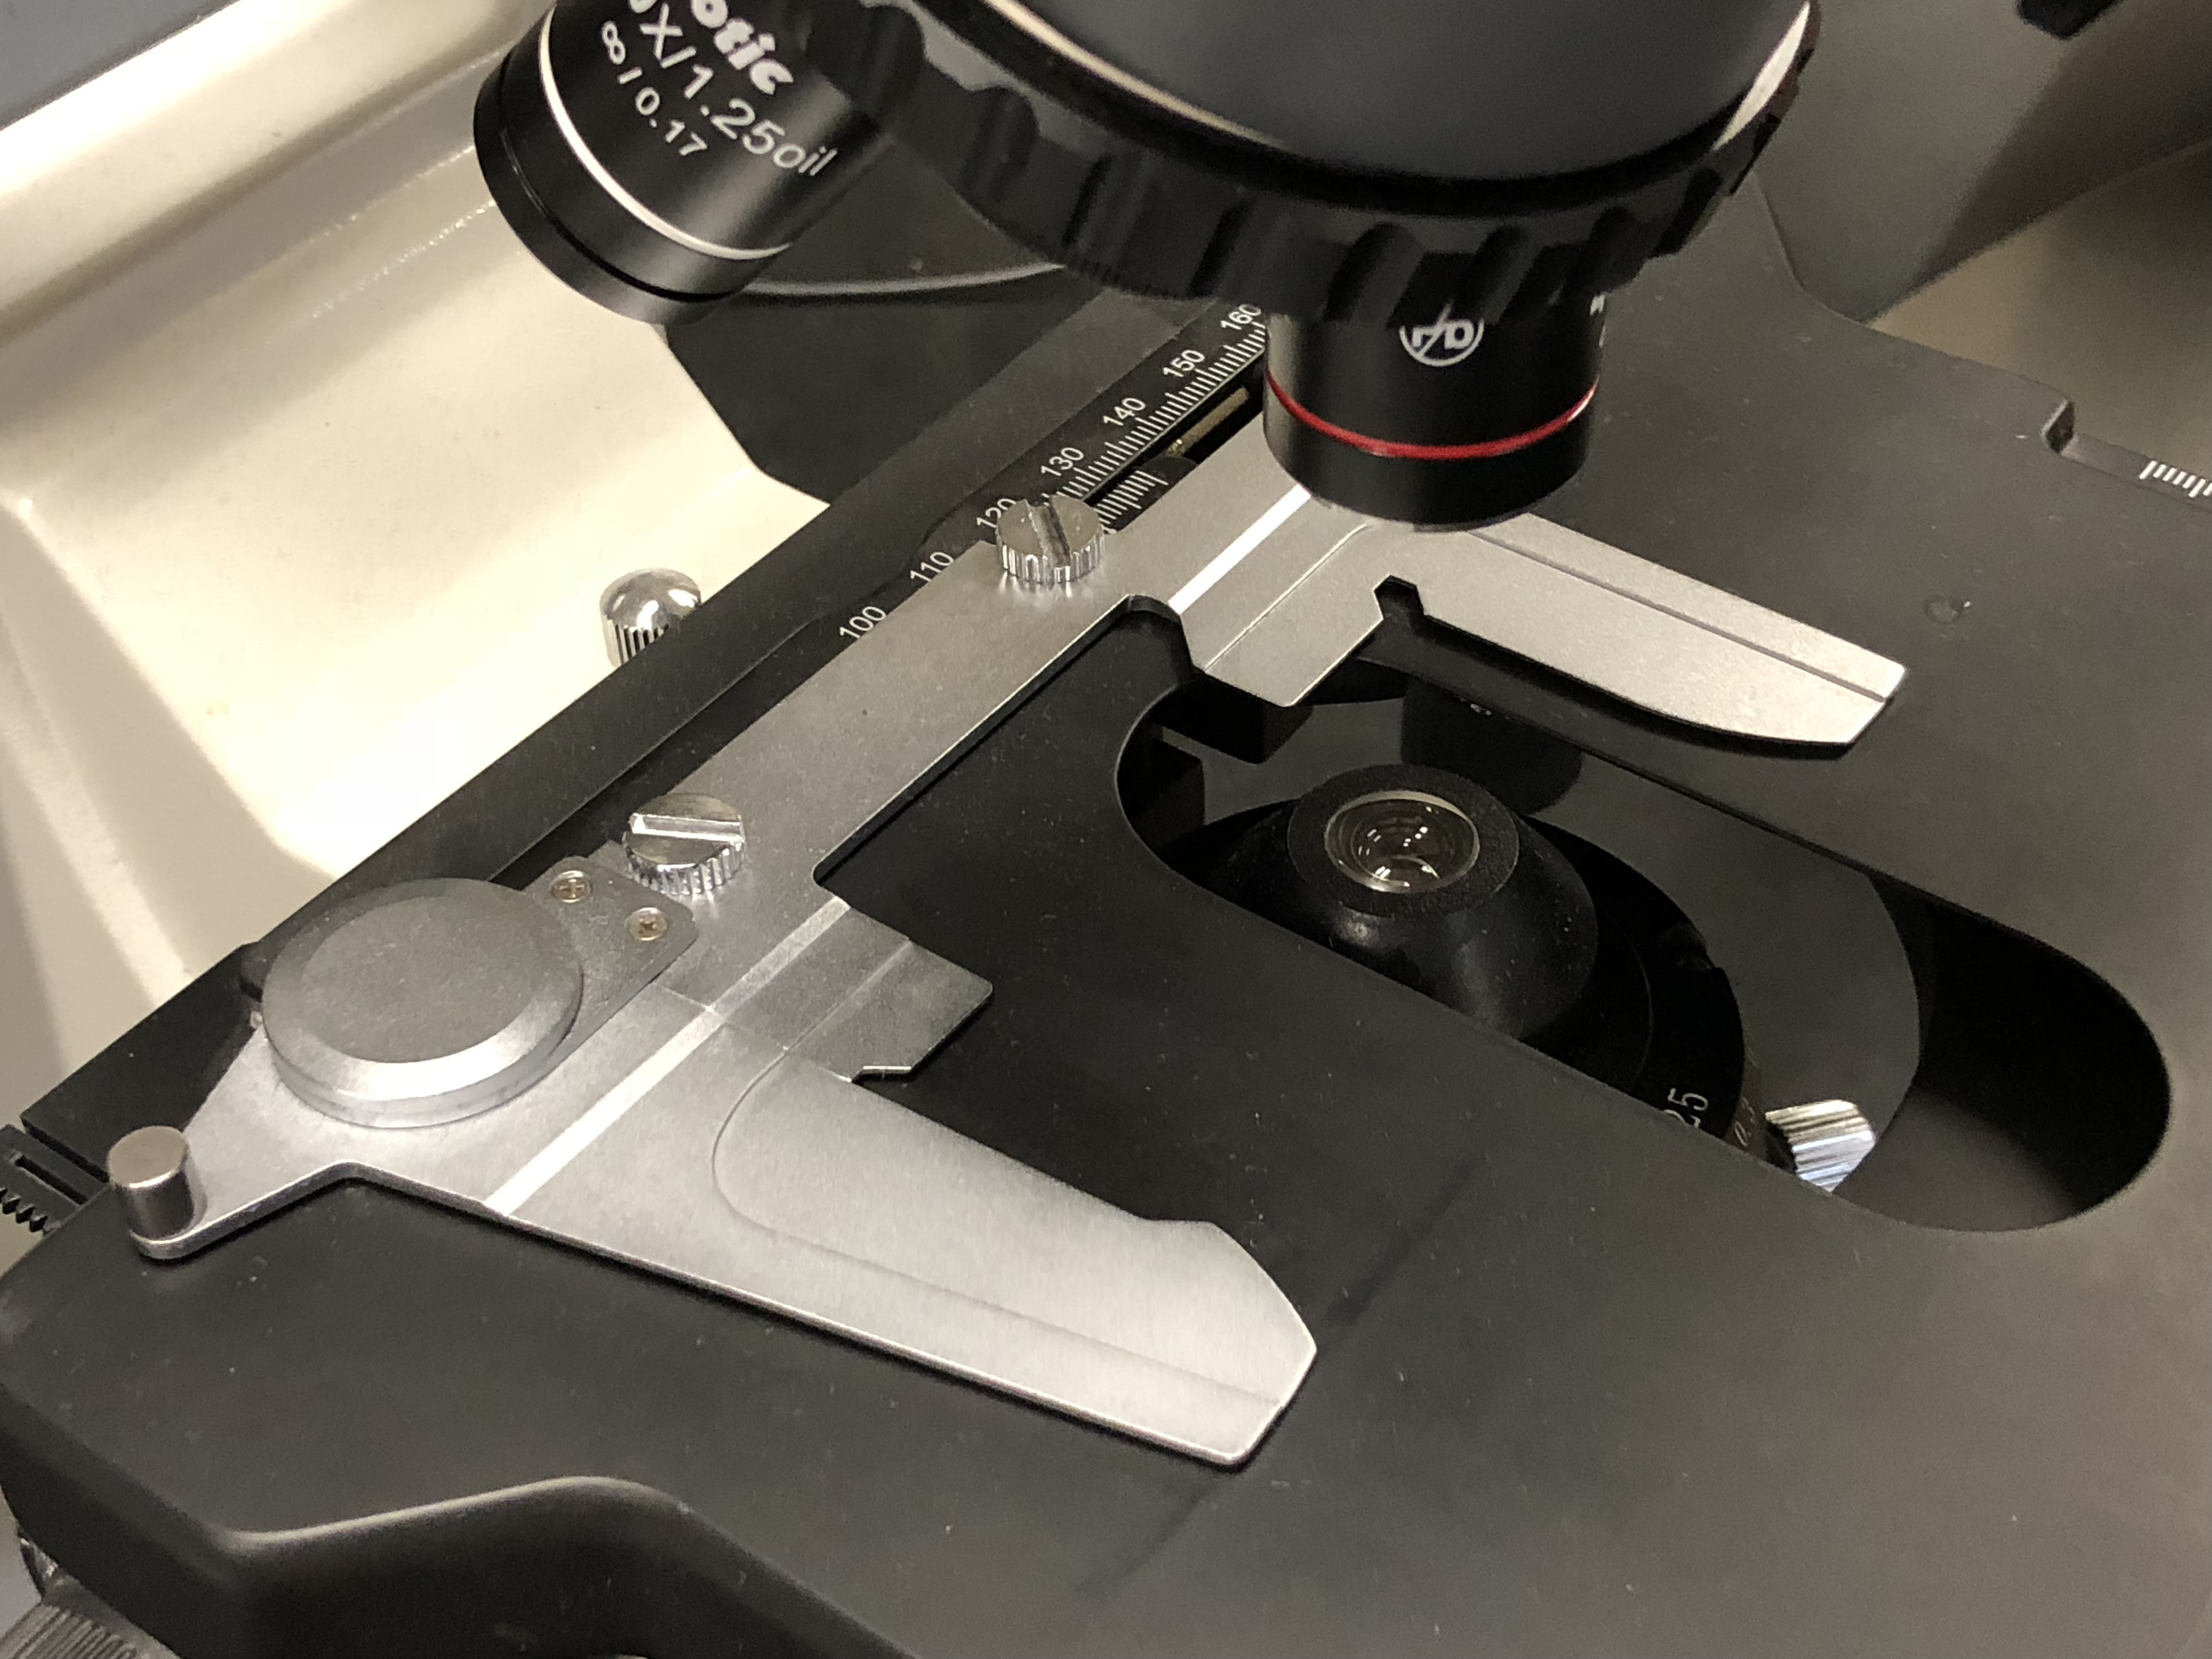
\includegraphics[width=0.7\linewidth]{./figures/microscope/stage} 

}

\caption{The stage with the slide holder and central opening showing the condenser lens.}\label{fig:stage}
\end{figure}

The stage moves up and down for focus. Always start with the lowest
magnification in order to center the specimen on the stage. After moving
to a higher magnification re-focus using the fine focus knob. You may
also have to adjust the horizontal positions using the horizontal stage
and slide holder adjustment knobs hanging down on the right side of the
stage (Figure \ref{fig:condenser}). Our microscopes, an adjustable LEDs
light source (knob on the right side). The condenser is a lens designed
to focus light from the illumination source onto the sample. The light
source and condenser also each include a diaphragm to influence the
quality and intensity of the illumination. For our purposes, the
diaphragms should always be completely open. Adjust the light intensity
only using the knob on the right side of the frame of the microscope
(the black knob below the green switch in Figure \ref{fig:stage}.

\begin{figure}

{\centering 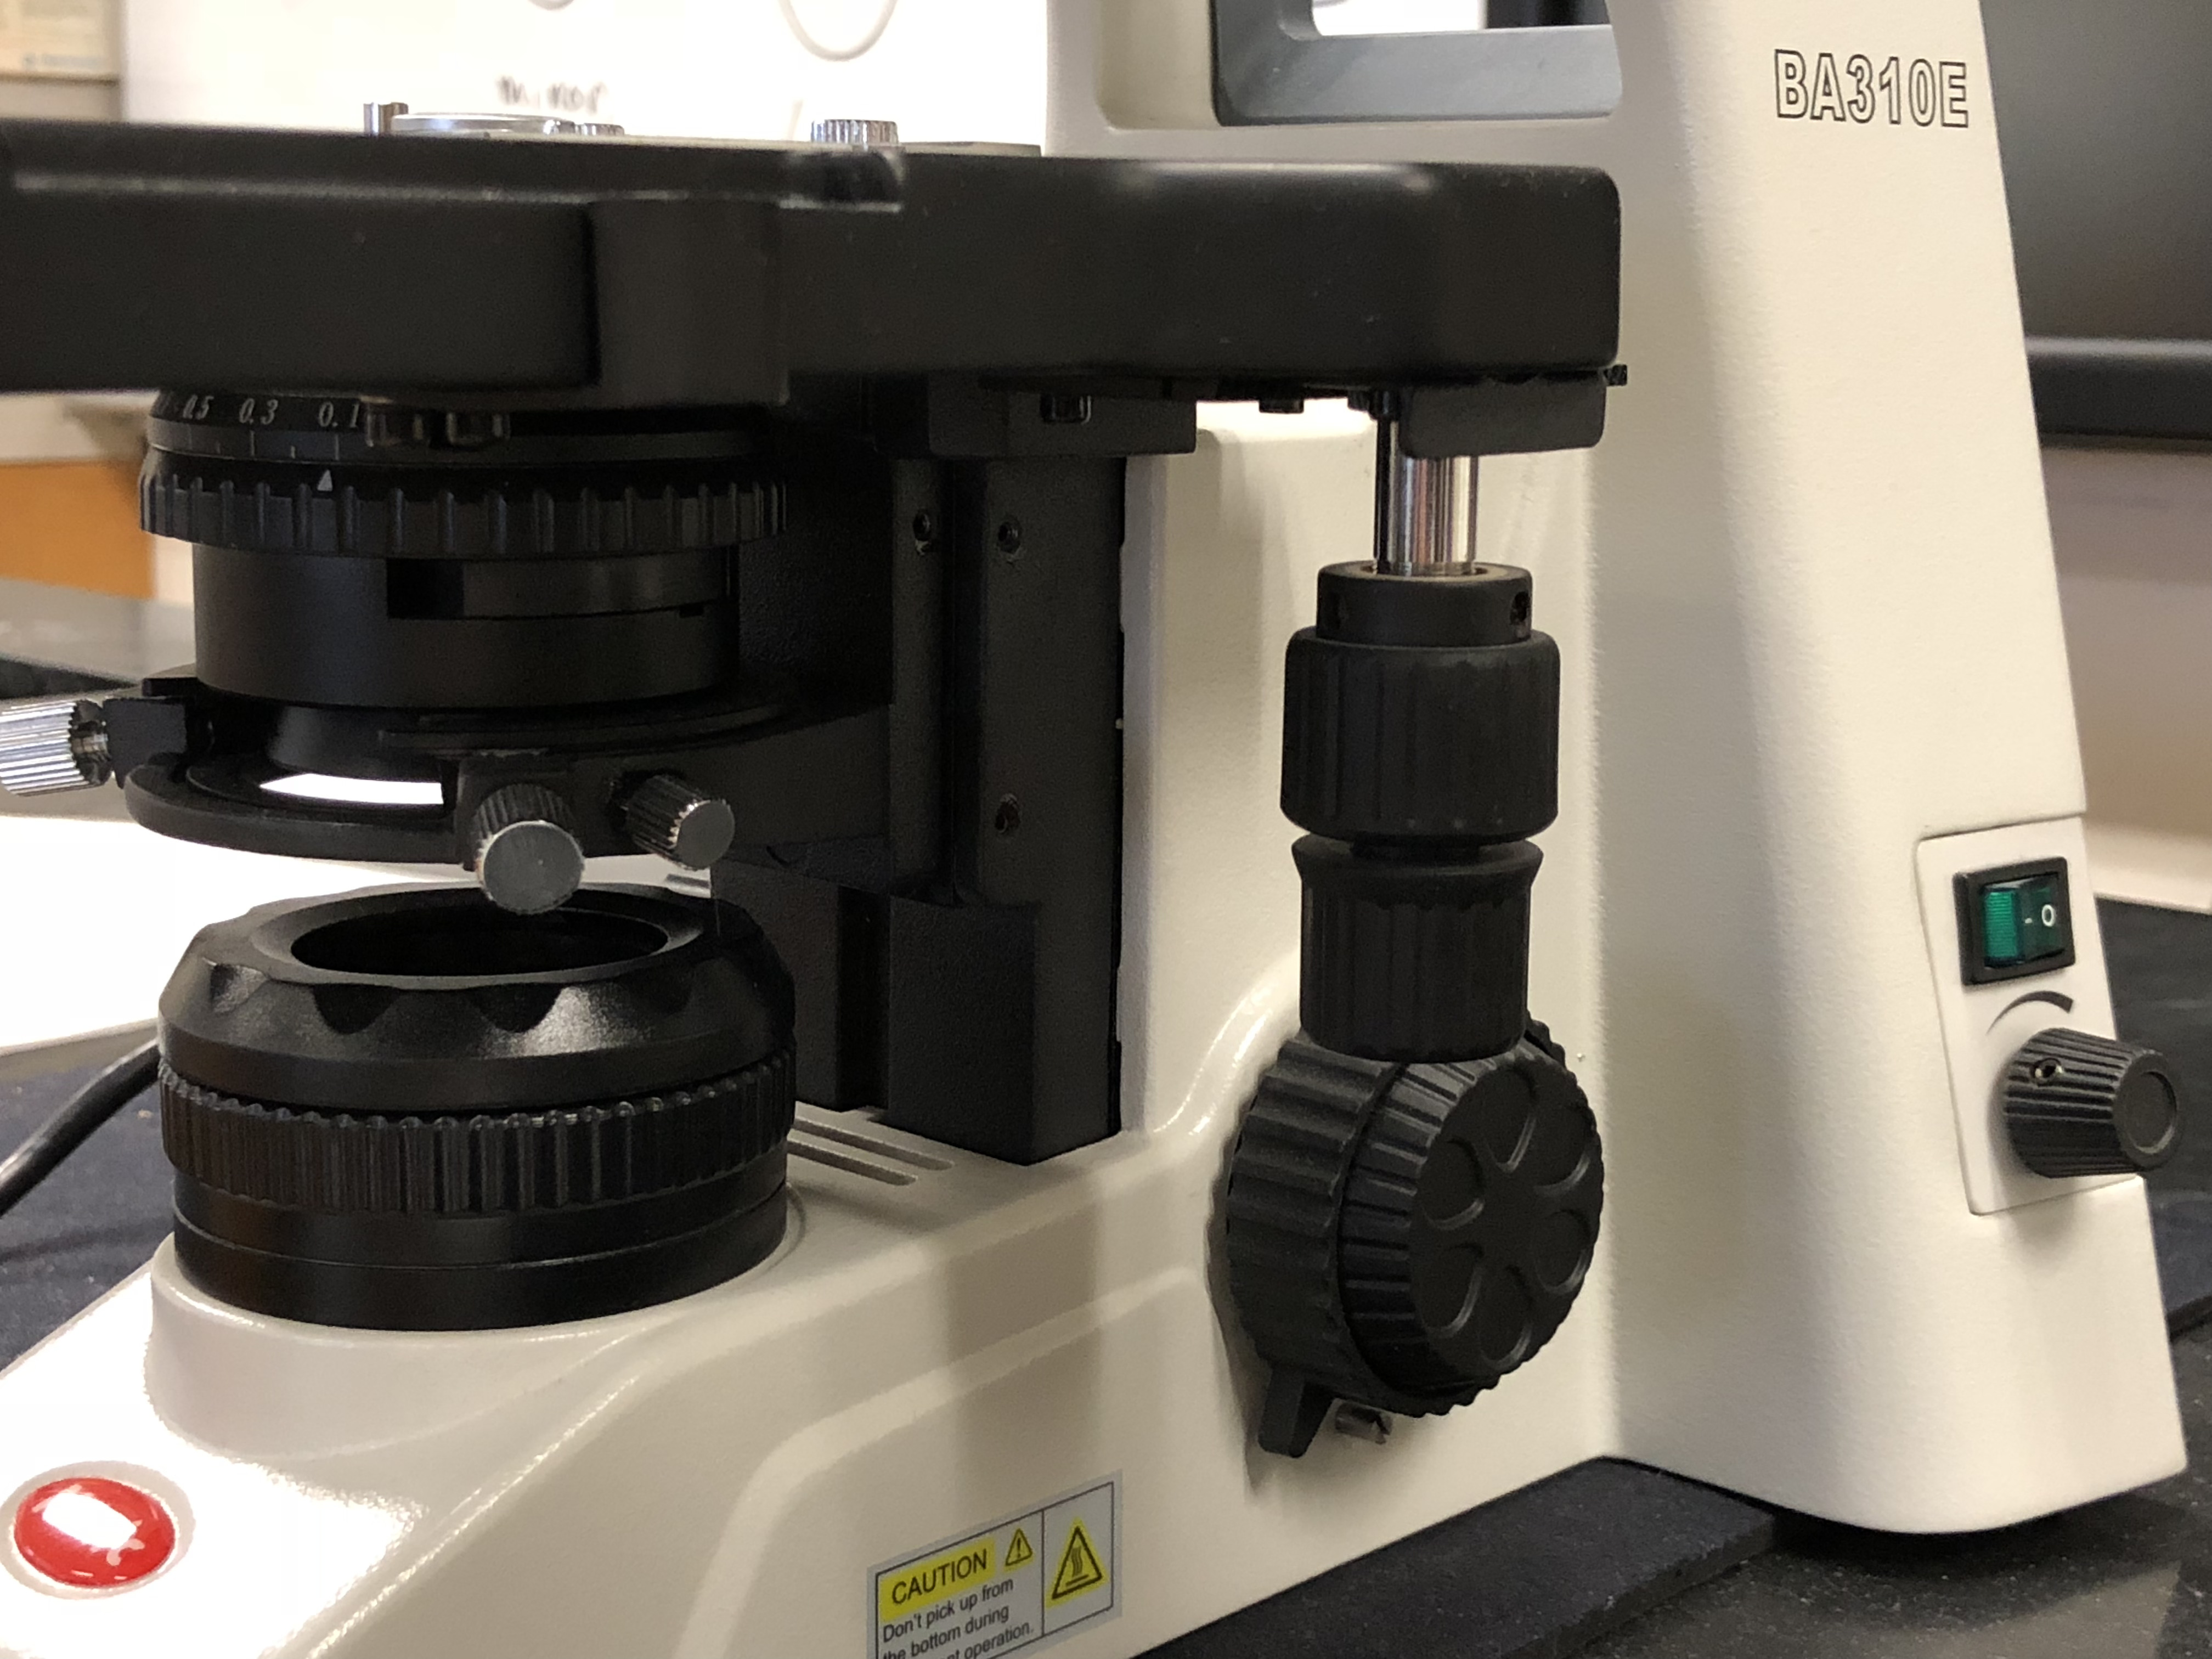
\includegraphics[width=0.7\linewidth]{./figures/microscope/condenser} 

}

\caption{The condenser (below the stage), the horizontal stage and slide holder adjustment knobs (hanging down from the stage), the light on switch and light intensity adjustment knob (in the back).}\label{fig:condenser}
\end{figure}

We have prepared a number of videos that introduce our microscopes to
you and also demonstrate how you can capture images of the slides that
you are viewing and transfer them to your own equipment.

\section{How to turn on the
microscope}\label{how-to-turn-on-the-microscope}

The tablets and microscopes must be turned on in a specific order:

\begin{enumerate}
\def\labelenumi{\arabic{enumi}.}
\tightlist
\item
  Microscope must be plugged in. If already plugged in, proceed to step
  3.
\item
  Motic logo will appear on tablet. After a few seconds, the charging
  symbol appears.
\item
  Press and hold the power button on the tablet for 6 seconds.
\item
  Motic symbol will appear again and tablet will start up.
\item
  Turn on microscope using the switch on the lower right side.
\end{enumerate}

\section{View Prepared Slides}\label{view-prepared-slides}

\begin{enumerate}
\def\labelenumi{\arabic{enumi}.}
\tightlist
\item
  Get a white slide box.
\item
  Clean all of the exposed lenses with special lens paper. Do not use
  paper towels, Kimwipes®, or cloth as this will scratch the lenses. If
  the view through the microscope becomes blurred, additional cleaning
  with lens paper may be necessary. Use alcohol pads if necessary.
\item
  Make sure that the low power objective is clicked into position.
\item
  Move the oculars as far apart from each other as possible then look
  through them with both eyes open. You will see two non-overlapping
  regions of light. Push the oculars slowly towards each other until you
  see one circle of light.
\item
  Always use both eyes when you look at slides. This will avoid eye
  strain and headaches.
\item
  Get the slide labelled ``Letter e'' (Figure \ref{fig:letter}) from the
  slide box.
\item
  Place the slide (coverslip up) on the stage and center the specimen
  over the opening in the stage.
\item
  Always start with the low power (4×) objective in place.
\item
  While looking through the ocular, use the coarse adjustment knob to
  slowly move the stage upward until the specimen comes into focus. If
  it does not, check to see that the material is centered on the stage,
  lower the stage, and try again.
\item
  Using the fine adjustment knob, obtain a sharp focus.
\item
  To increase the magnification, be sure the area you wish to examine
  specifically is in the center of the field; then, watching from the
  side to be sure that the objective clears the slide, turn the
  nose-piece until the next higher power objective clicks into position.
  The material now should be in view and should require only slight
  focusing with the fine adjustment. Never focus with the coarse
  adjustment under high power.
\item
  What happens when you increase the magnification?
\item
  Before removing the slide, always return the microscope to low power
  and turn the coarse adjustment knob until the stage is moved all the
  way down.
\item
  View the computer chip slide (Figure \ref{fig:chip}).
\item
  View the colored threads slide (Figure \ref{fig:threads}).
\item
  Which thread is at the bottom, in the middle, on top?
\item
  Depth perception requires that a slightly different angle of an object
  is seen by the left and right eye. This happens because of the
  horizontal separation parallax of the eyes. If an object is far away,
  the disparity of that image falling on both retinas will be small. If
  the object is close or near, the disparity will be large. The
  microscope presents the same view to both eyes. Therefore, the only
  way to answer the above question is to change the focus of the image
  and observe what happens: when you move the stage upwards, to bring
  the slide closer to the objective, the thread that is on top will come
  into focus first, the middle one second and the bottom one last. Try
  it and write down your answer!

  \begin{itemize}
  \tightlist
  \item
    Bottom thread: \_\_\_\_\_\_\_\_\_\_
  \item
    Middle thread: \_\_\_\_\_\_\_\_\_\_
  \item
    Top thread: \_\_\_\_\_\_\_\_\_\_
  \end{itemize}
\item
  View the stage micrometer slide (Figure \ref{fig:scale}).
\item
  What is the unit of this scale?
\item
  What is the distance between 1.0 and 1.5 in meters?
\item
  How many subdivisions can you distinguish between 0 and 0.1?
\item
  What is the distance in meters between the smallest subdivision?
\item
  View the blood smear slide (Figure \ref{fig:smear}).
\item
  Which cells are red blood cells? Mark with an arrow and label it
  ``RBC''.
\item
  Which cells are white blood cells? Mark with an arrow and label it
  ``WBC''.
\item
  Return the slides to the slide boxes and the slide boxes to the bench
  where you picked it up.
\end{enumerate}

\begin{figure}

{\centering 
\includegraphics[width=0.7\linewidth]{./figures/microscope/Letter_e} 

}

\caption{A printed letter.}\label{fig:letter}
\end{figure}

\begin{figure}

{\centering 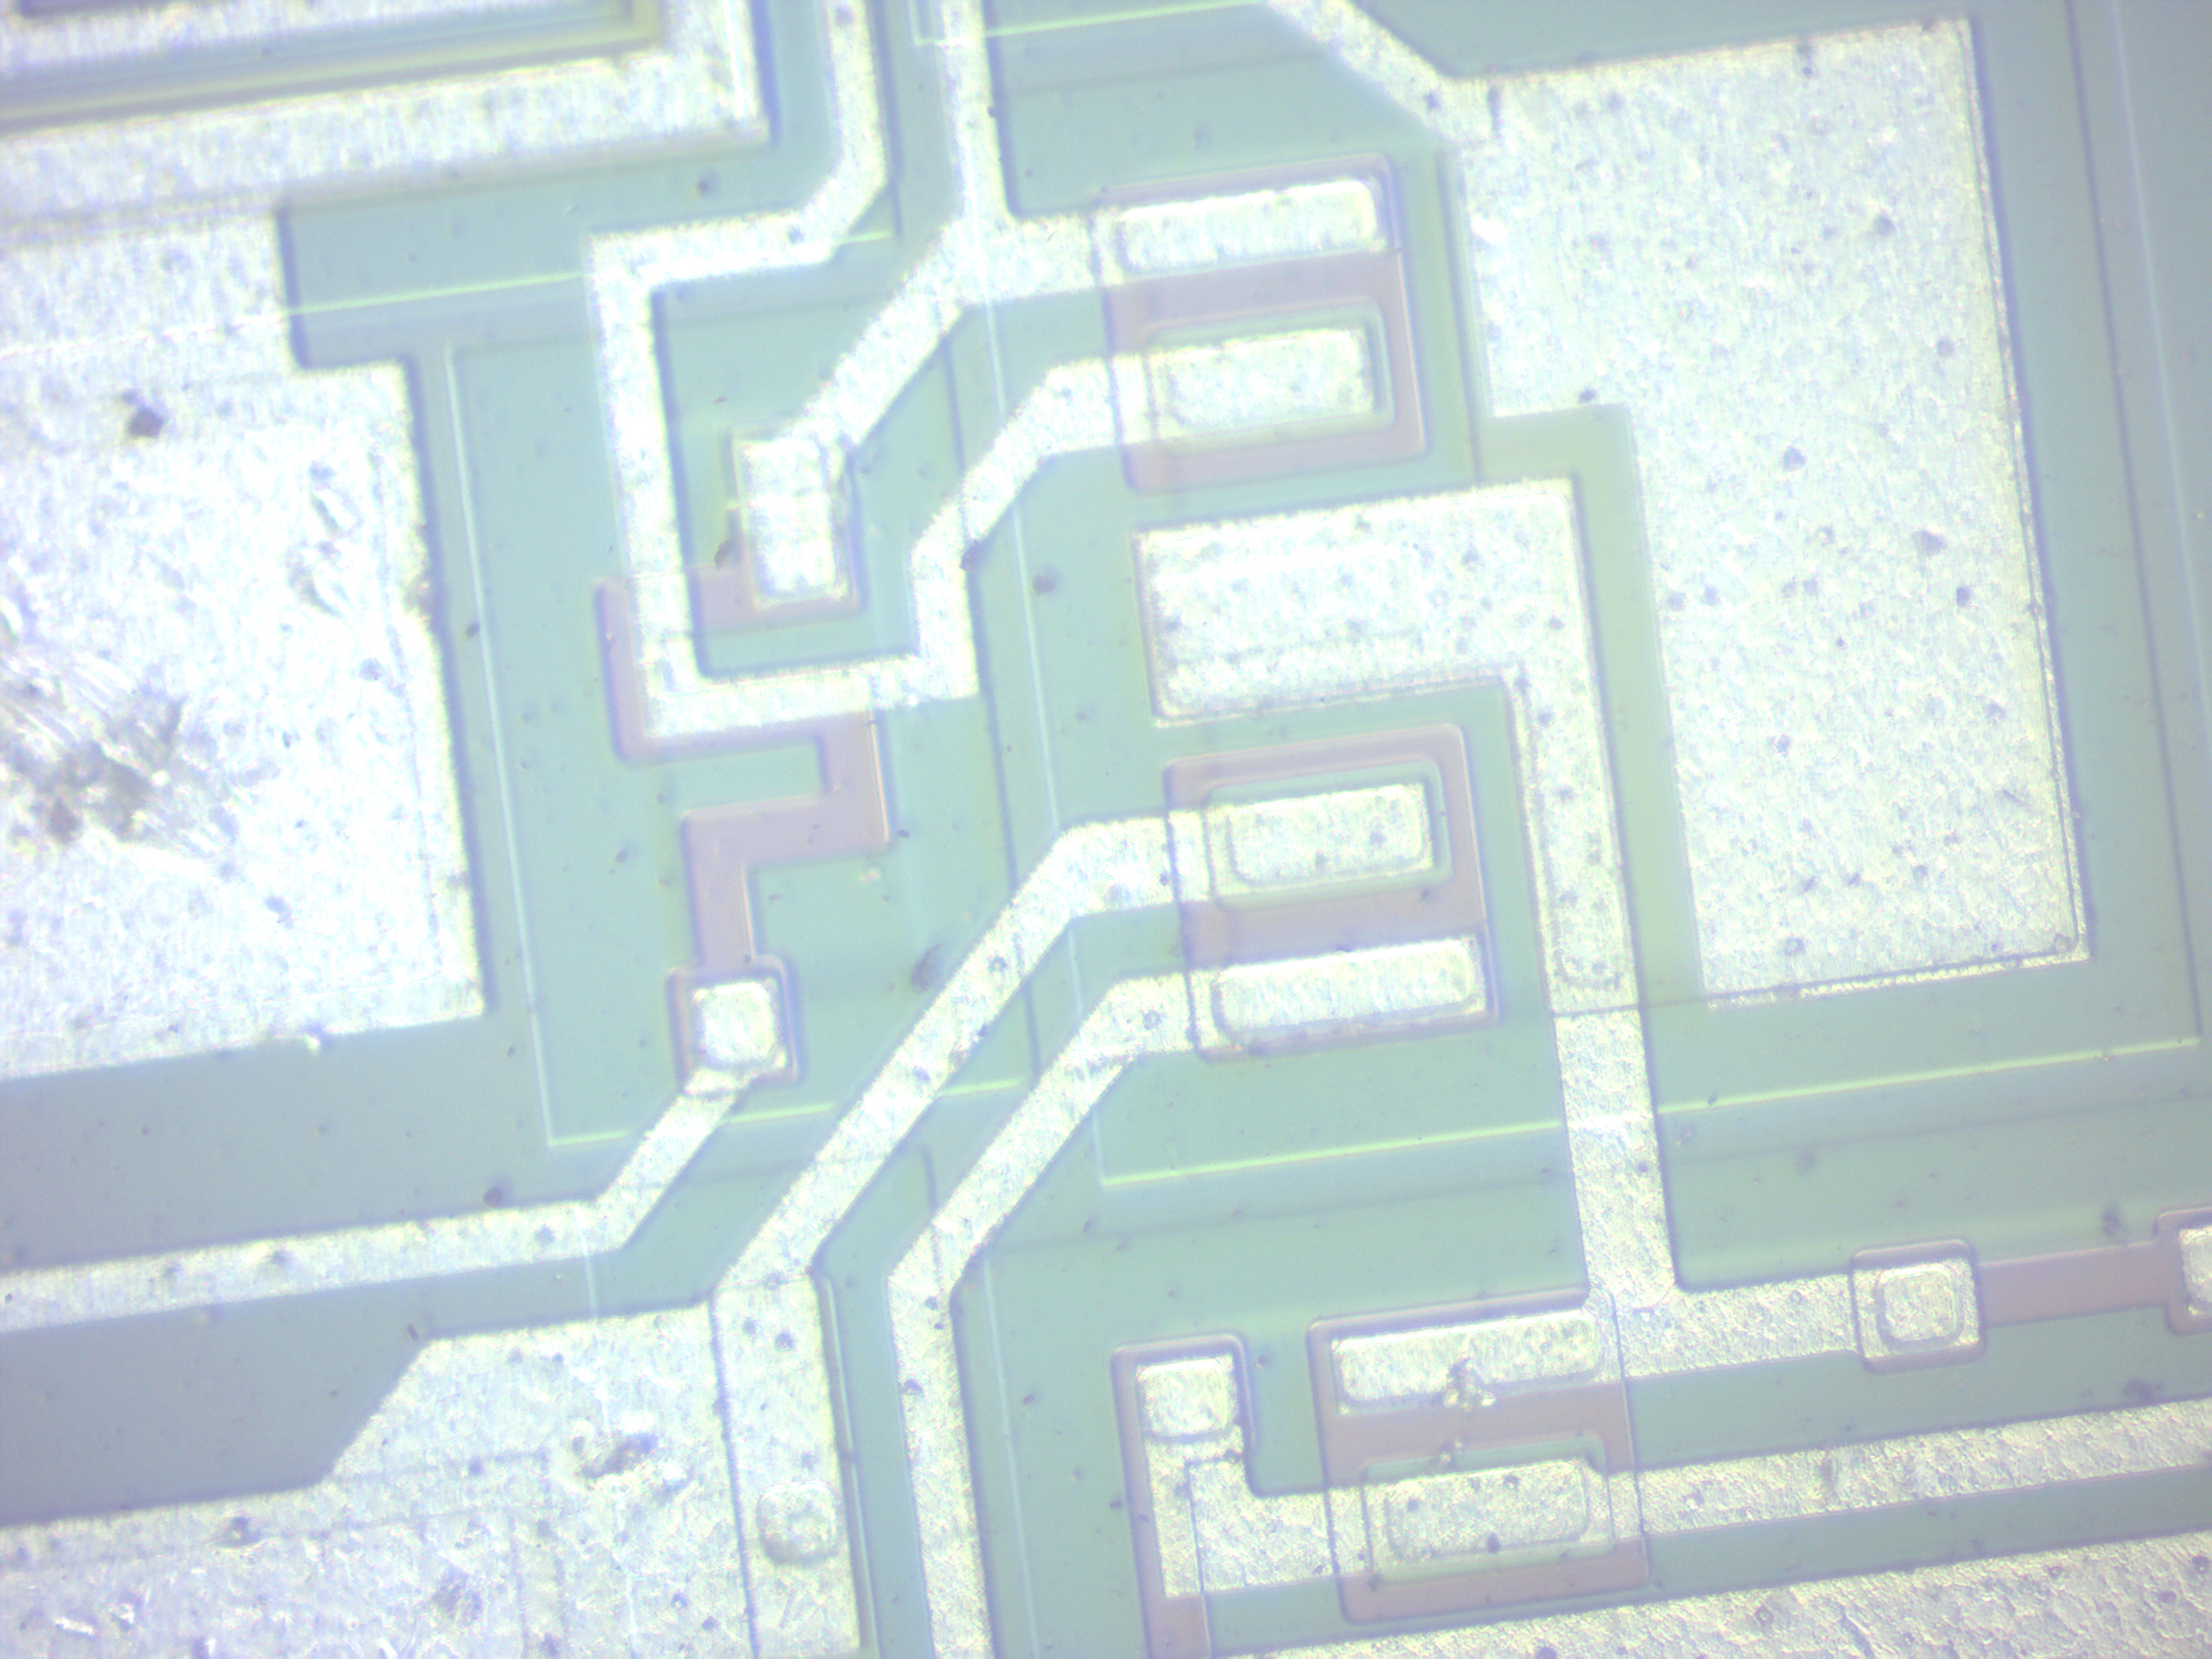
\includegraphics[width=0.7\linewidth]{./figures/microscope/Chip} 

}

\caption{Close-up view of an electronic chip.}\label{fig:chip}
\end{figure}

\begin{figure}

{\centering 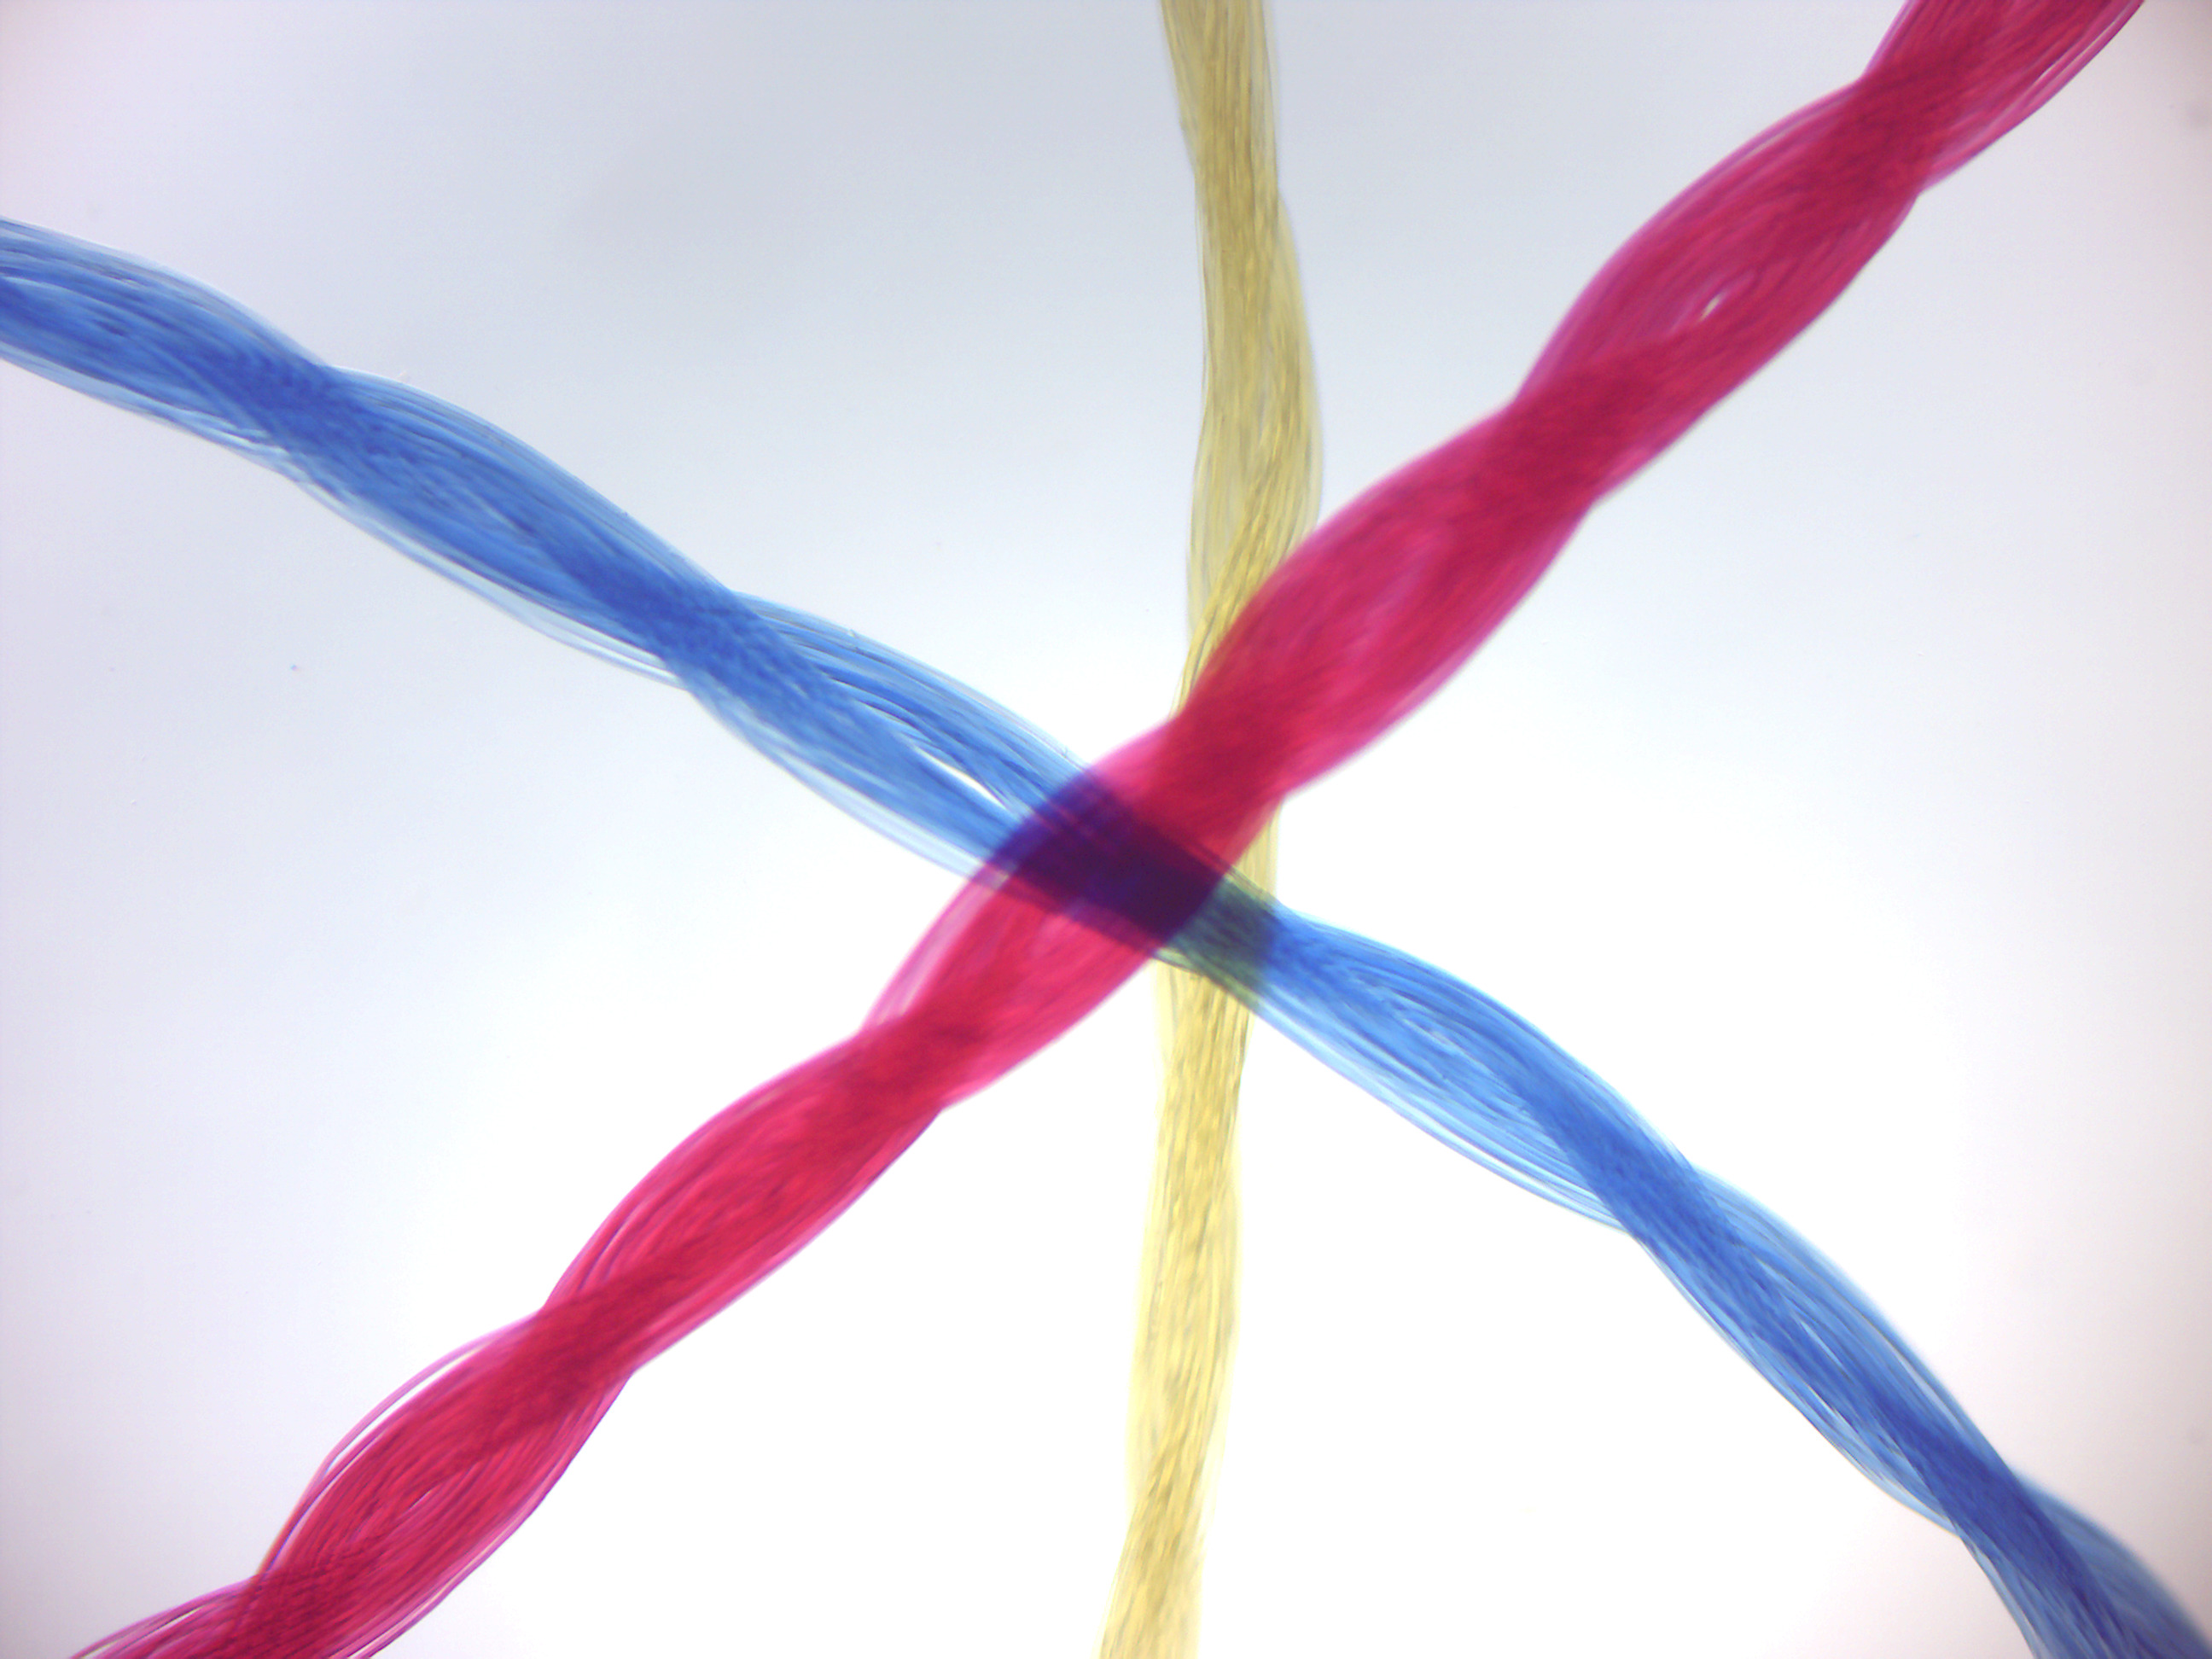
\includegraphics[width=0.7\linewidth]{./figures/microscope/Threads} 

}

\caption{Which thread is on top, in the middle, at the bottom?}\label{fig:threads}
\end{figure}

\begin{figure}

{\centering 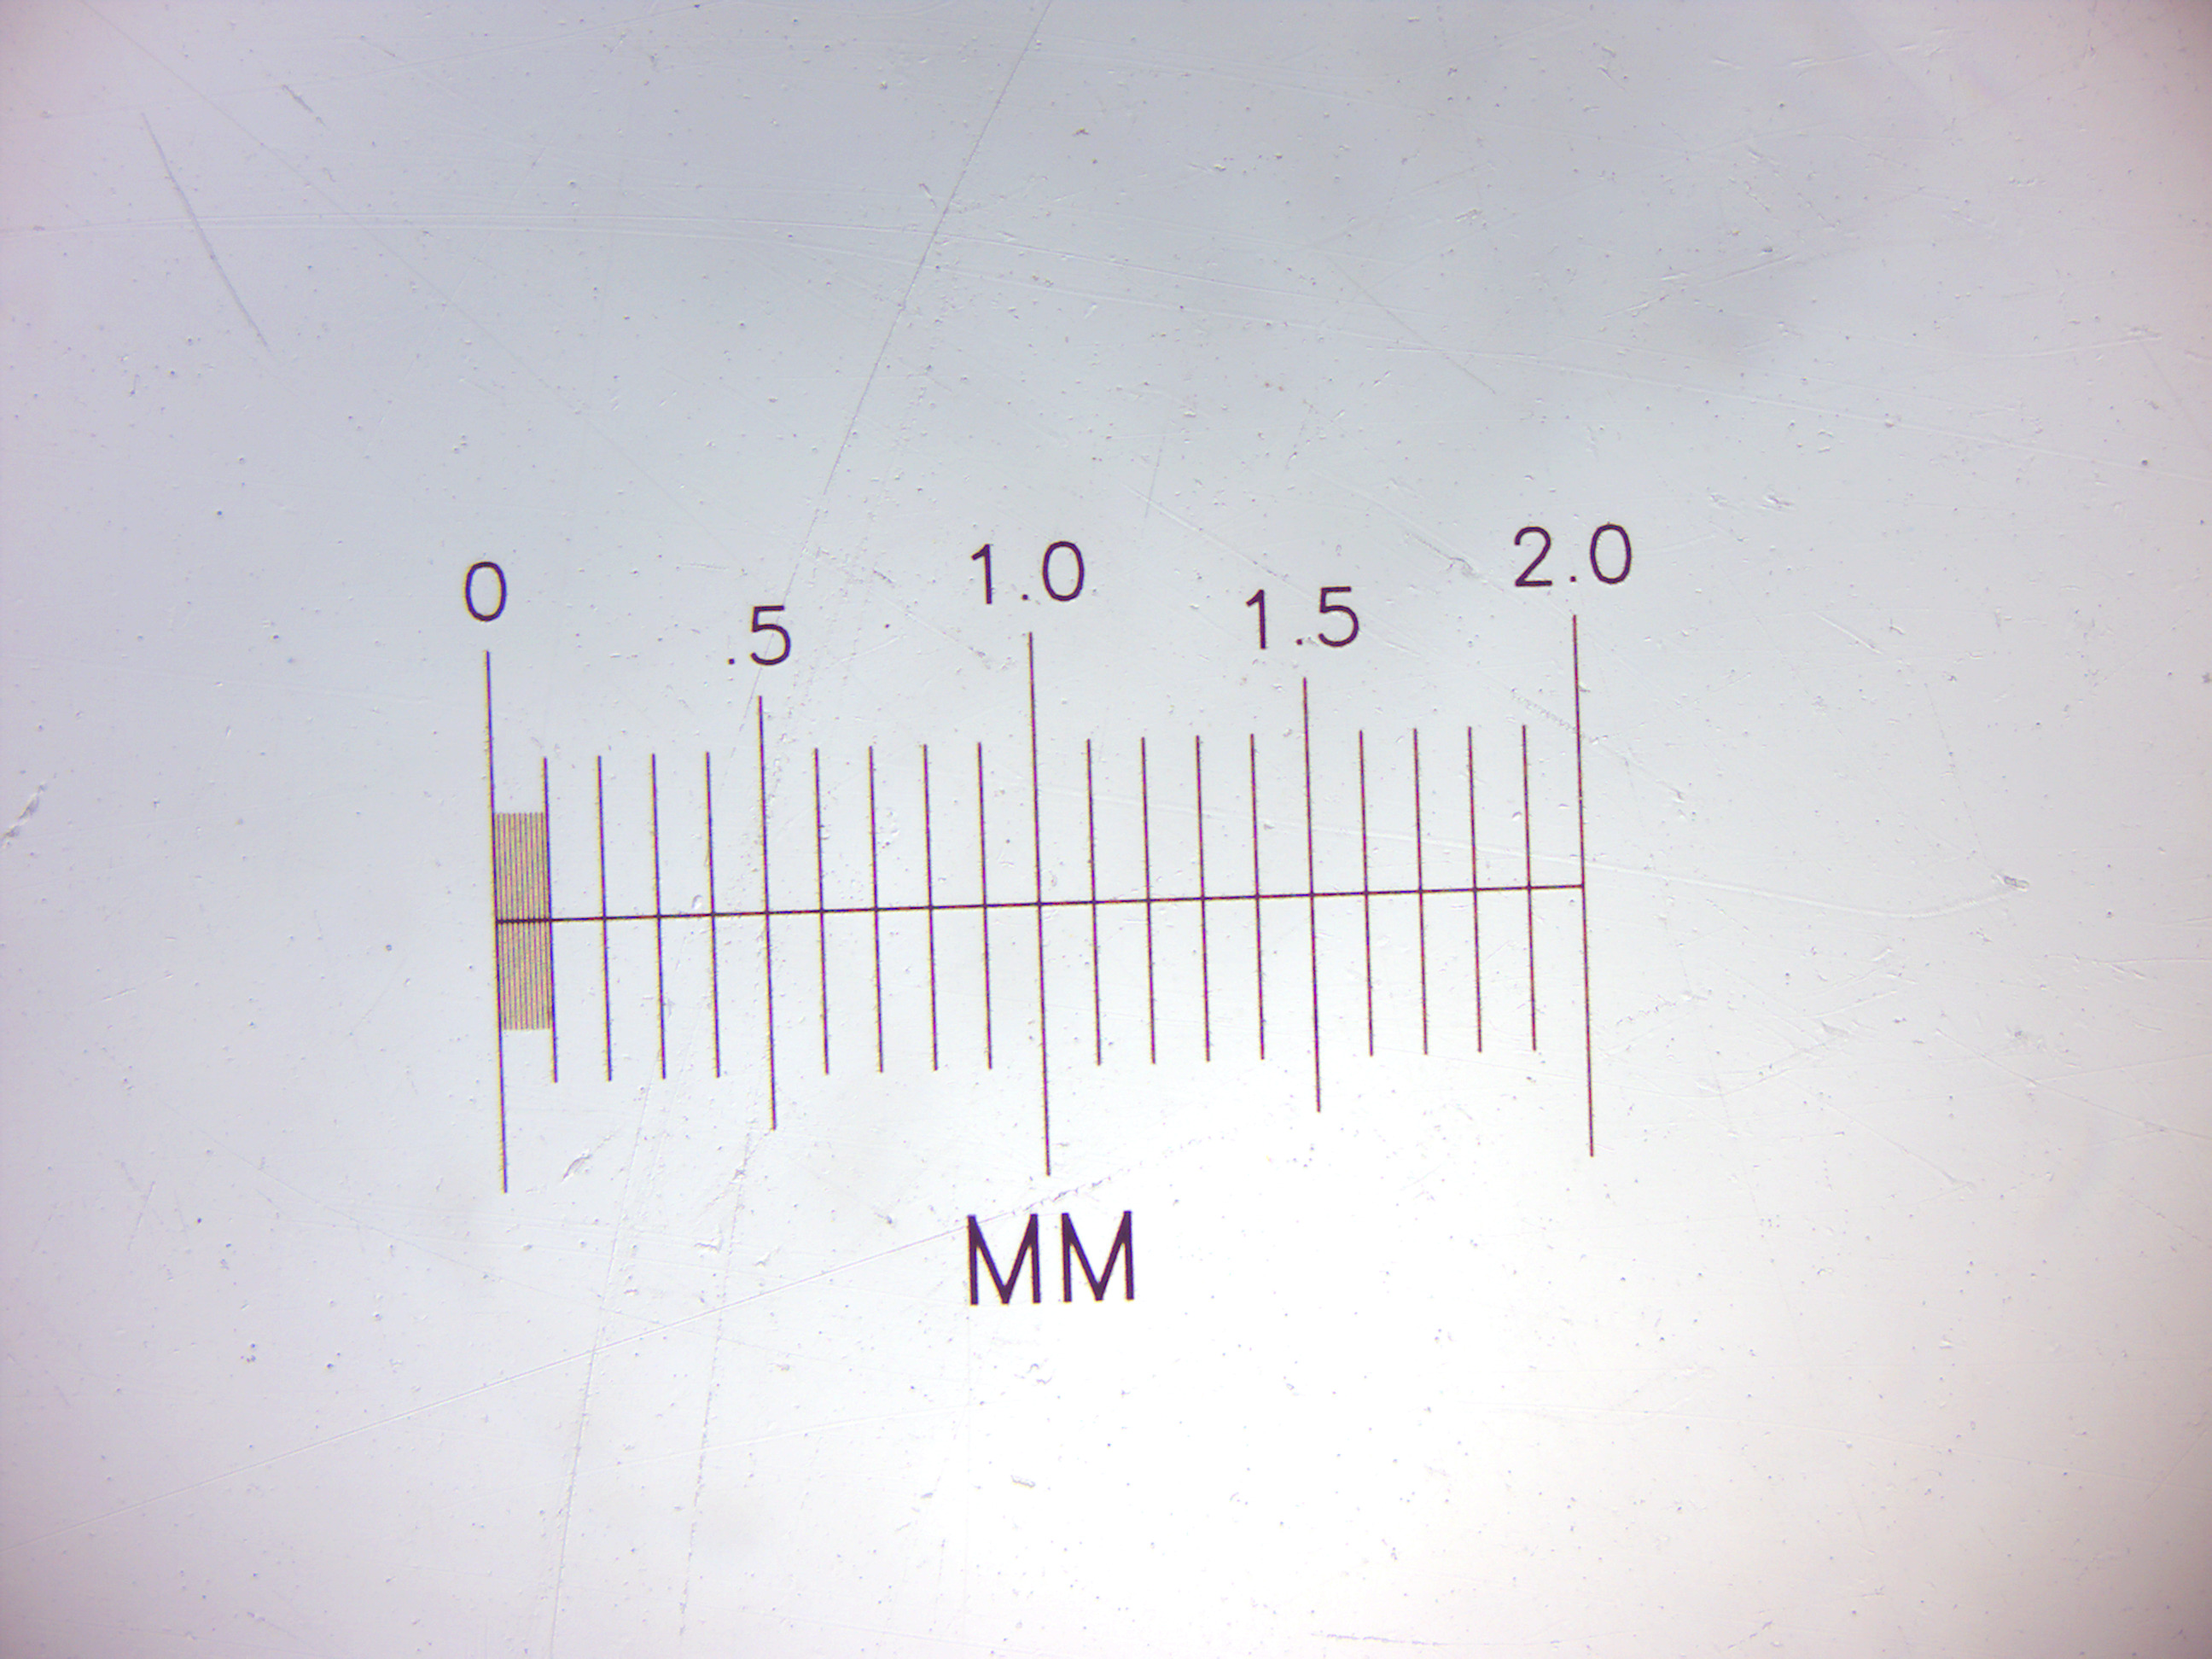
\includegraphics[width=0.7\linewidth]{./figures/microscope/MM_scale} 

}

\caption{A microscopic scale.}\label{fig:scale}
\end{figure}

\begin{figure}

{\centering 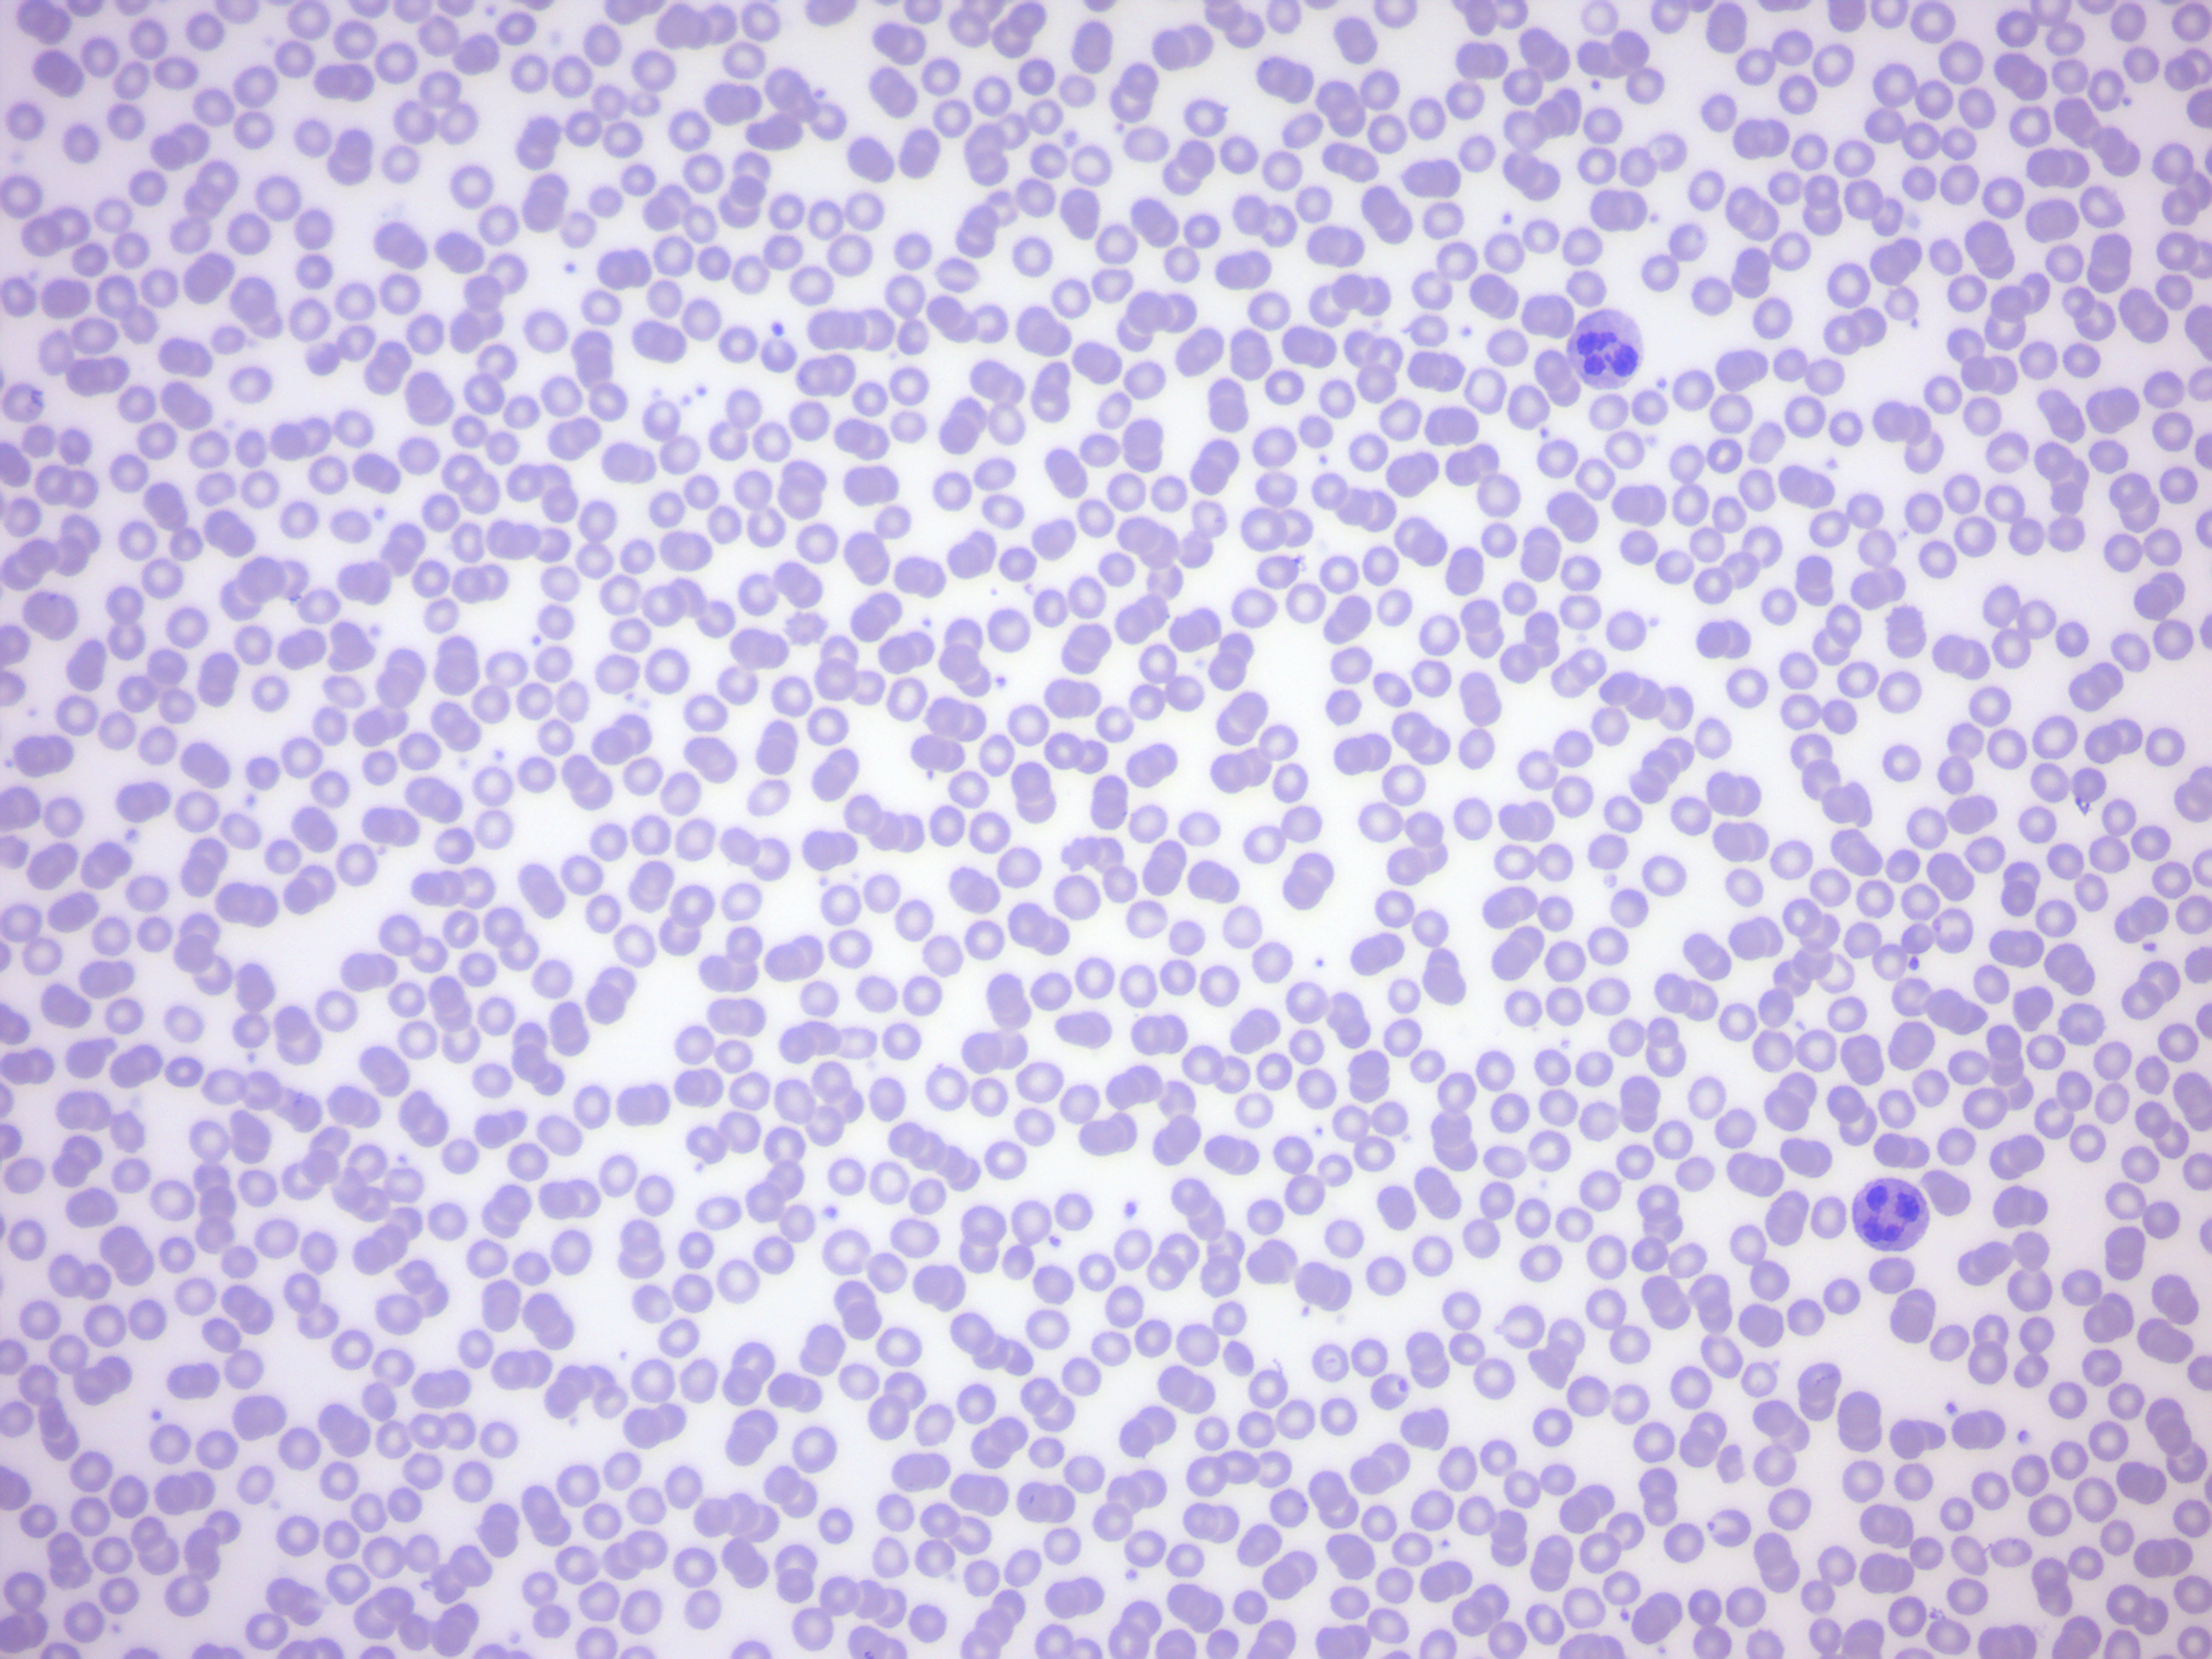
\includegraphics[width=0.7\linewidth]{./figures/microscope/Blood_smear} 

}

\caption{A human blood smear.}\label{fig:smear}
\end{figure}

\section{Elodea Leaf Wet Mount}\label{elodea-leaf-wet-mount}

\href{https://en.wikipedia.org/wiki/Elodea_canadensis}{\emph{Elodea
canadensis}} (American or Canadian waterweed or pondweed) is a perennial
aquatic plant, or submergent macrophyte, native to most of North
America. It grows rapidly in favorable conditions and can choke shallow
ponds, canals, and the margins of some slow-flowing rivers. It requires
summer water temperatures of 10-25 °C and moderate to bright lighting.
Young plants initially start with a seedling stem with roots growing in
mud at the bottom of the water; further adventitious roots are produced
at intervals along the stem, which may hang free in the water or anchor
into the bottom. It grows indefinitely at the stem tips, and single
specimens may reach lengths of 3 m or more. The leaves are bright green,
translucent, oblong, 6-17 mm long and 1-4 mm broad, borne in whorls of
three (rarely two or four) round the stem. It lives entirely underwater,
the only exception being the small white or pale purple flowers which
float at the surface and are attached to the plant by delicate stalks.
It is dioecious, with male and female flowers on different plants. The
flowers have three small white petals; male flowers have 4.5-5 mm petals
and nine stamens, female flowers have 2-3 mm petals and three fused
carpels. The fruit is an ovoid capsule, about 6 mm long containing
several seeds that ripen underwater. The seeds are 4-5 mm long,
fusiform, glabrous (round), and narrowly cylindrical. It flowers from
May to October.

\subsection{Experimental procedures}\label{experimental-procedures}

\begin{enumerate}
\def\labelenumi{\arabic{enumi}.}
\tightlist
\item
  Get a single leaf from the Elodea plant and mount it on a slide, cover
  it with a drop of water and a cover slip.
\item
  Place the slide onto the microscope state and observe at the leaf
  under the microscope.
\item
  These leaves are two cells thick, so you should be able to focus up
  and down to see that the cells in one layer are larger than those in
  the other. When one layer is in focus, you may be able to see the
  shadowy outlines of cell walls in the other layer.
\item
  Notice that the cells are clearly delineated by the cell wall.
\item
  Inside the cells are large oval-shaped green bodies, the chloroplasts.
\item
  As the cells warm, you can see the chloroplasts carried by the moving
  cytoplasm around the nearly transparent nucleus in the center of the
  cell.
\item
  Make a drawing of what you see at 400× magnification.
\end{enumerate}

\section{How to turn off the
microscope}\label{how-to-turn-off-the-microscope}

The tablets and microscopes must be turned off in a specific order:

\begin{enumerate}
\def\labelenumi{\arabic{enumi}.}
\tightlist
\item
  Turn off microscope using the switch on the lower right side.
\item
  While the microscope is still plugged in, turn off the tablet by
  holding the power button down for a few seconds. Select power off.
\item
  Motic logo will appear on tablet.
\item
  Wait till charging symbol will appear.
\item
  Leave microscopes kept on the student bench plugged in after turning
  them off and place the cover over the microscope.
\end{enumerate}

\section{Review Questions}\label{review-questions}

\begin{enumerate}
\def\labelenumi{\arabic{enumi}.}
\tightlist
\item
  Why do biologists use microscopes?
\item
  What is the function of the microscope objectives?
\item
  What are the magnification factors of the objectives of our
  microscopes?
\item
  What is the name of the lenses that are close to your eyes when you
  look through the microscope?
\item
  What is the magnifying power of these lenses?
\item
  What is the total magnification of the image that you observe if you
  use the 40× objective?
\item
  What is the difference between the action of the coarse and the fine
  focus knobs?
\item
  Which part of the microscope moves when you turn the focus knobs?
\item
  What is the field of view?
\item
  How does it change when you switch from a lower to a higher power
  objective?
\end{enumerate}

\chapter{Chemical Aspects of Life}\label{chemical-aspects-of-life}

\href{https://en.wikipedia.org/wiki/Matter}{Everything that we can bump
into, touch or squeeze including living things are composed of atoms.}
\href{https://en.wikipedia.org/wiki/Chemical_element}{Chemical elements}
are pure substances of one type of
\href{https://en.wikipedia.org/wiki/Atom}{atom}. Atoms combine to form
\href{https://en.wikipedia.org/wiki/Molecule}{molecules}. Molecules
combined of more than one element are called compounds.

Commonly people distinguish between organic and inorganic compounds.
However, there is no clear or universally agreed-upon distinction
between organic and inorganic compounds. Organic chemists traditionally
and generally refer to any molecule containing carbon as an organic
compound and by default this means that inorganic chemistry deals with
molecules lacking carbon. As many minerals are of biological origin,
biologists may distinguish organic from inorganic compounds in a
different way that does not hinge on the presence of a carbon atom.
Pools of organic matter, for example, that have been metabolically
incorporated into living tissues persist in decomposing tissues, but as
molecules become oxidized into the open environment, such as atmospheric
CO\textsubscript{2}, this creates a separate pool of inorganic
compounds. The International Union of Pure and Applied Chemistry
(IUPAC), an agency widely recognized for defining chemical terms, does
not offer definitions of inorganic or organic compounds. Hence, the
definition for an inorganic versus an organic compound in a
multidisciplinary context spans the division between organic life living
(or animate) and inorganic non-living (or inanimate) matter. In broader
speech, the term commonly referred to compounds synthesized by purely
geological systems, in contrast to those with a biological component in
their origin.

Cells consist mostly of water (70\%-90\%). The bulk of their dry weight
consists of compounds containing the elements carbon (C), hydrogen (H),
oxygen (O), nitrogen (N), and phosphorus (P). The four major types of
organic biomolecules are carbohydrates, lipids, proteins and nucleic
acids. The more complex members of these categories (biomacromolecules)
are made up of chains of smaller molecules (monomers) strung together
more or less like beads in a necklace. These complex molecules are
called polymers. In living organisms, polymers are made by dehydration
synthesis, the loss of a water molecule between each pair of monomers.
Conversely, polymers can be digested (broken up into monomers) by the
addition of a molecule of water between each pair of monomers. This
process is known as hydrolysis.

Carbohydrates are biomolecules consisting of carbon (C), hydrogen (H)
and oxygen (O) atoms, usually with a hydrogen to oxygen atom ratio of
2:1 (as in water) with the formula
C\textsubscript{n}(H\textsubscript{2}O)\textsubscript{n}.

Lipids are substances of biological origin that are insoluble in water.
Lipids comprise a group of naturally occurring molecules that include
fats, waxes, sterols, fat-soluble vitamins (such as vitamins A, D, E,
and K), monoglycerides, diglycerides, triglycerides, and phospholipids.
The main biological functions of lipids include storing energy,
signaling, and acting as structural components of cell membranes.

Proteins are large biomolecules consisting of one or more long chains of
amino acids linked by peptide bonds. Proteins perform a vast array of
functions within organisms, including catalyzing metabolic reactions,
DNA replication, responding to stimuli, and transporting molecules from
one location to another. Proteins differ from one another primarily in
their sequence of amino acids, which is dictated by the nucleotide
sequence of their genes, and which usually results in protein folding
into a specific three-dimensional structure that determines its
activity.

\begin{figure}

{\centering 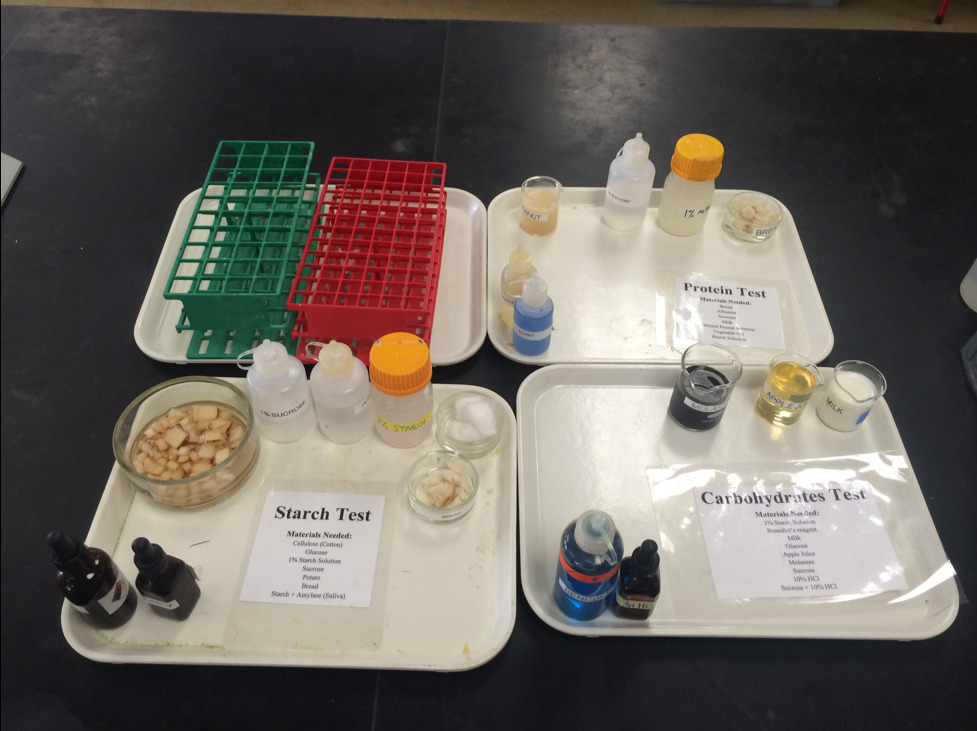
\includegraphics[width=0.7\linewidth]{./figures/chem_aspects/Setup} 

}

\caption{Experimental materials for this lab}\label{fig:setup}
\end{figure}

\section{Test for Reducing sugars}\label{test-for-reducing-sugars}

A \href{https://en.wikipedia.org/wiki/Reducing_sugar}{reducing sugar} is
one that reduces another compound and is itself oxidized; that is, the
carbonyl carbon of the sugar is oxidized to a carboxyl group. A reducing
sugar has a free aldehyde group or a free ketone group. All
monosaccharides are reducing sugars, along with some disaccharides,
oligosaccharides, and polysaccharides. Monosaccharides which contain an
aldehyde group are known as aldoses, and those with a ketone group are
known as ketoses. The aldehyde can be oxidized via a redox reaction in
which another compound is reduced. Thus, a reducing sugar is one that
reduces certain chemicals. Sugars with ketone groups in their open chain
form are capable of isomerizing via a series of tautomeric shifts to
produce an aldehyde group in solution. Therefore, ketone-bearing sugars
like fructose are considered reducing sugars but it is the isomer
containing an aldehyde group which is reducing since ketones cannot be
oxidized without decomposition of the sugar. This type of isomerization
is catalyzed by the base present in solutions which test for the
presence of aldehydes. Aldoses or aldehyde-bearing sugars are reducing
also because during oxidation of aldoses, there are certain oxidizing
agents that are reduced. The common dietary monosaccharides galactose,
glucose and fructose are all reducing sugars. Many disaccharides, like
lactose and maltose, also have a reducing form, as one of the two units
may have an open-chain form with an aldehyde group. However, sucrose is
a non-reducing disaccharide since neither of the rings is capable of
opening. Benedict's reagent (Cu\textsuperscript{2+} in aqueous sodium
citrate) is used as a qualitative test to detect the presence of
reducing sugars. The reducing sugar reduces the copper(II) ions to
copper(I), which then forms a brick red copper(I) oxide precipitate.

\begin{figure}

{\centering 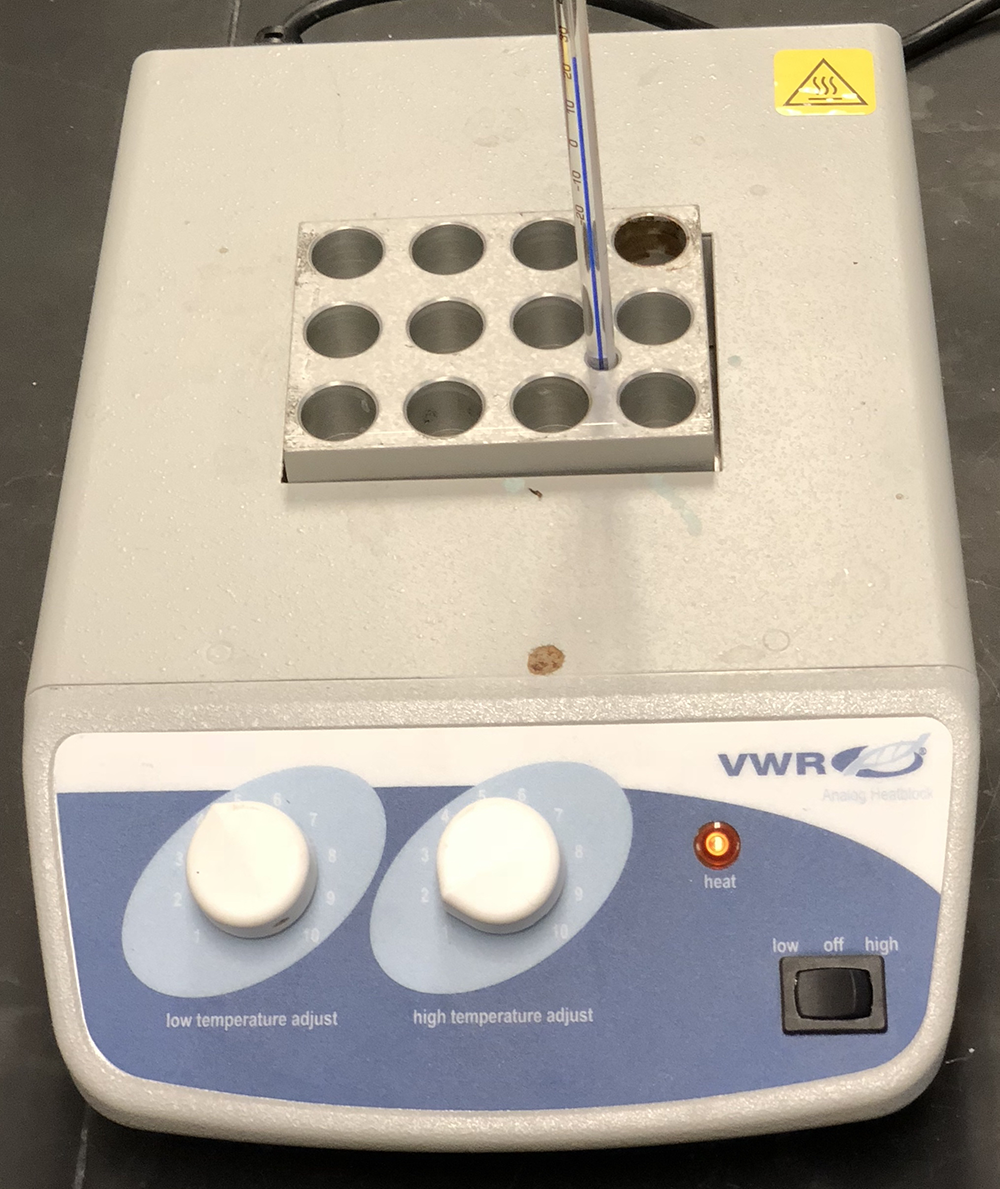
\includegraphics[width=0.7\linewidth]{./figures/chem_aspects/Heatblock} 

}

\caption{Heat block ("dry bath")}\label{fig:heatblock}
\end{figure}

\subsection{Experimental procedures}\label{experimental-procedures-1}

\begin{enumerate}
\def\labelenumi{\arabic{enumi}.}
\tightlist
\item
  Turn on the 65 °C heat block (Figure \ref{fig:heatblock}) by pushing
  the little black switch on the lower right side of the to ``high''.
  Rotate the white ``high temperature adjust'' button to number 3.
\item
  Turn on the 37 °C heat block by pushing the little black switch on the
  lower right side of the to ``low''. Rotate the white ``low temperature
  adjust'' button to number 4.
\item
  Obtain 7 plastic test tubes and a test tube rack.
\item
  Using a wax pencil,label each tube with a number (1 to 7).
\item
  Place the tubes from left (tube \#1) to right (tube \#7) in the first
  row of a test tube rack.
\item
  Add the test material each tube as indicated in Table \ref{tab:sugar}.
\item
  Add 2 ml of Benedict's reagent to each tube using a plastic transfer
  pipette. Figure 5 Plastic transfer pipette (3 ml capacity.
\item
  Mix well.
\item
  Check the that the temperature of the heat block is
  \textasciitilde{}65 °C and then place the tubes in the heat block. Set
  a timer and incubate the tubes for 15 minutes. Begin setting up
  Experiment 2 (below) while the tubes are incubating.
\item
  After 15 minutes, remove the tubes using a test tube holder (be
  careful, they are hot!), place them in the tube rack and record the
  color (in your own words) in Table \ref{tab:sugar}.
\end{enumerate}

\begin{longtable}[]{@{}clccc@{}}
\caption{\label{tab:sugar} Test for reducing sugars.}\tabularnewline
\toprule
Tube \# & Test material & Benedict's & Observed color & Test Result (+
or -)\tabularnewline
\midrule
\endfirsthead
\toprule
Tube \# & Test material & Benedict's & Observed color & Test Result (+
or -)\tabularnewline
\midrule
\endhead
1 & 2 ml H\textsubscript{2}O & 2 ml & &\tabularnewline
2 & 2 ml glucose & 2 ml & &\tabularnewline
3 & 2 ml milk & 2 ml & &\tabularnewline
4 & 2 ml apple juice & 2 ml & &\tabularnewline
5 & 2 ml starch & 2 ml & &\tabularnewline
6 & 2 ml molasses & 2 ml & &\tabularnewline
7 & 2 ml sucrose & 2 ml & &\tabularnewline
\bottomrule
\end{longtable}

\begin{figure}

{\centering 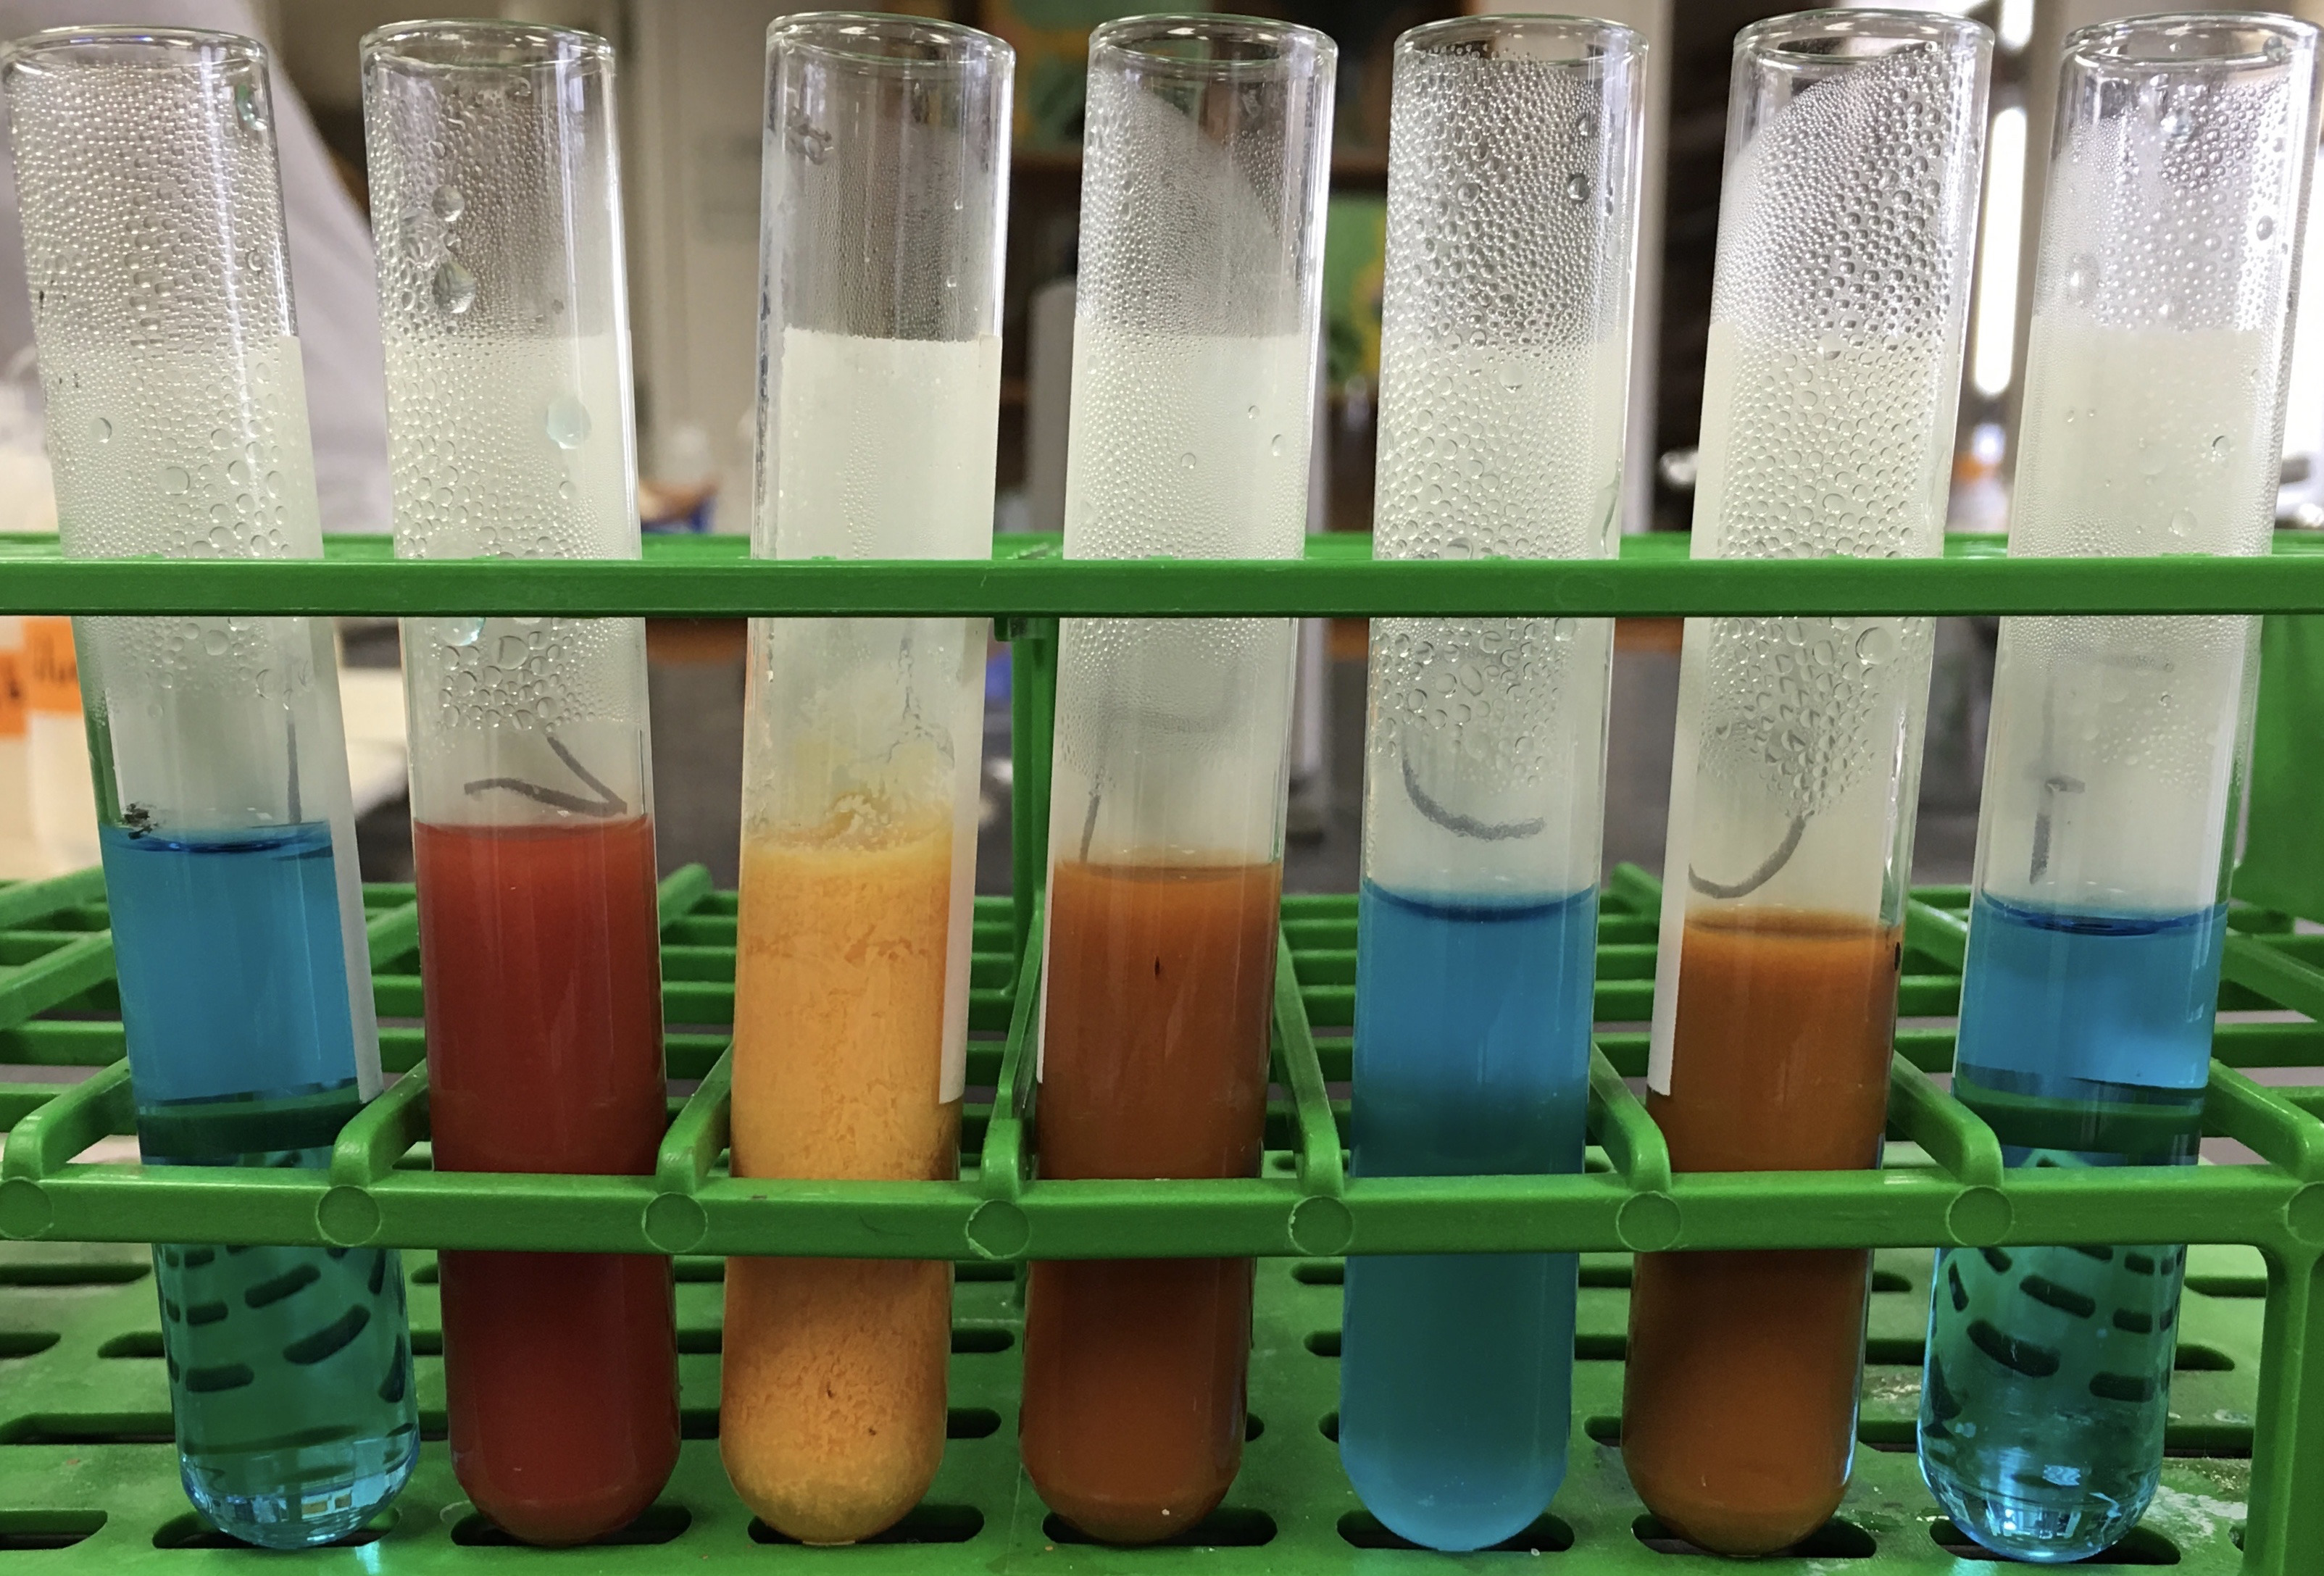
\includegraphics[width=0.7\linewidth]{./figures/chem_aspects/Results_exp_1} 

}

\caption{Results from experiment 1. Compare to your results!}\label{fig:exp1}
\end{figure}

\section{Test for Starch}\label{test-for-starch}

Starch is a polymeric carbohydrate consisting of a large number of
glucose units joined by glycosidic bonds. This polysaccharide is
produced by most green plants as energy storage. It is the most common
carbohydrate in human diets and is contained in large amounts in staple
foods like potatoes, wheat, maize (corn), rice, and cassava. Pure starch
is a white, tasteless and odorless powder that is insoluble in cold
water or alcohol. It consists of two types of molecules the linear and
helical amylose and the branched amylopectin.

An \href{https://en.wikipedia.org/wiki/Amylase}{amylase} is an enzyme
that catalyzes the hydrolysis of starch into maltose and glucose.
Amylase is present in the saliva of humans, where it begins the chemical
process of digestion. It is also produced by the pancreas.

\subsection{Experimental procedures}\label{experimental-procedures-2}

\begin{enumerate}
\def\labelenumi{\arabic{enumi}.}
\tightlist
\item
  Obtain 9 plastic test tubes and a test tube rack.
\item
  Using a wax pencil,label each tube with a number (1 to 9).
\item
  Place the tubes from left (tube \#1) to right (tube \#9) in the first
  row of a test tube rack.
\item
  Add the test material to tubes 1 to 8 as indicated in the table below.
  Leave tube 9 empty.
\item
  Check the that the temperature of the heat block is
  \textasciitilde{}37 °C and then place tube \#8 in the heat block. Set
  a timer and incubate the tubes for 15 minutes.
\item
  Add 5 drops of Iodine solution to the test tubes \#1 to \# 7. Mix
  well.
\item
  Record the color (in your own words) in in Table \ref{tab:starch}.
\item
  After 15 minutes, remove test tube 8 from the heat block and transfer
  2 ml (half of the contents of test tube 8) to tube 9.
\item
  Add 5 drops of iodine to tube 8 and record your observation in Table
  \ref{tab:starch}.
\item
  Add 2 ml of Benedict's solution to tube \#9.
\item
  Place tube 9 in the \textasciitilde{}65 °C heat block. Set a timer and
  incubate the tube for 15 minutes.
\item
  After 15 minutes, remove tube 9 using a test tube holder (be careful,
  it is hot!), place it in the tube rack and record the color (in your
  own words) in the table.
\end{enumerate}

\begin{longtable}[]{@{}clccc@{}}
\caption{\label{tab:starch} Test for starch.}\tabularnewline
\toprule
Tube \# & Test material & Iodine & Observed color & Test Result (+ or
-)\tabularnewline
\midrule
\endfirsthead
\toprule
Tube \# & Test material & Iodine & Observed color & Test Result (+ or
-)\tabularnewline
\midrule
\endhead
1 & 2 ml starch & 5 drops & &\tabularnewline
2 & 2 ml glucose & 5 drops & &\tabularnewline
3 & 2 ml H\textsubscript{2}O & 5 drops & &\tabularnewline
4 & 2 ml sucrose & 5 drops & &\tabularnewline
5 & cotton (cellulose) & 5 drops & &\tabularnewline
6 & a small piece of bread & 5 drops & &\tabularnewline
7 & a small piece of potato & 5 drops & &\tabularnewline
8 & 2 ml of starch plus 2 ml of amylase & 5 drops & &\tabularnewline
9 & Leave empty then follow step 8 above & 2 ml of Benedict's solution &
&\tabularnewline
\bottomrule
\end{longtable}

\begin{figure}

{\centering 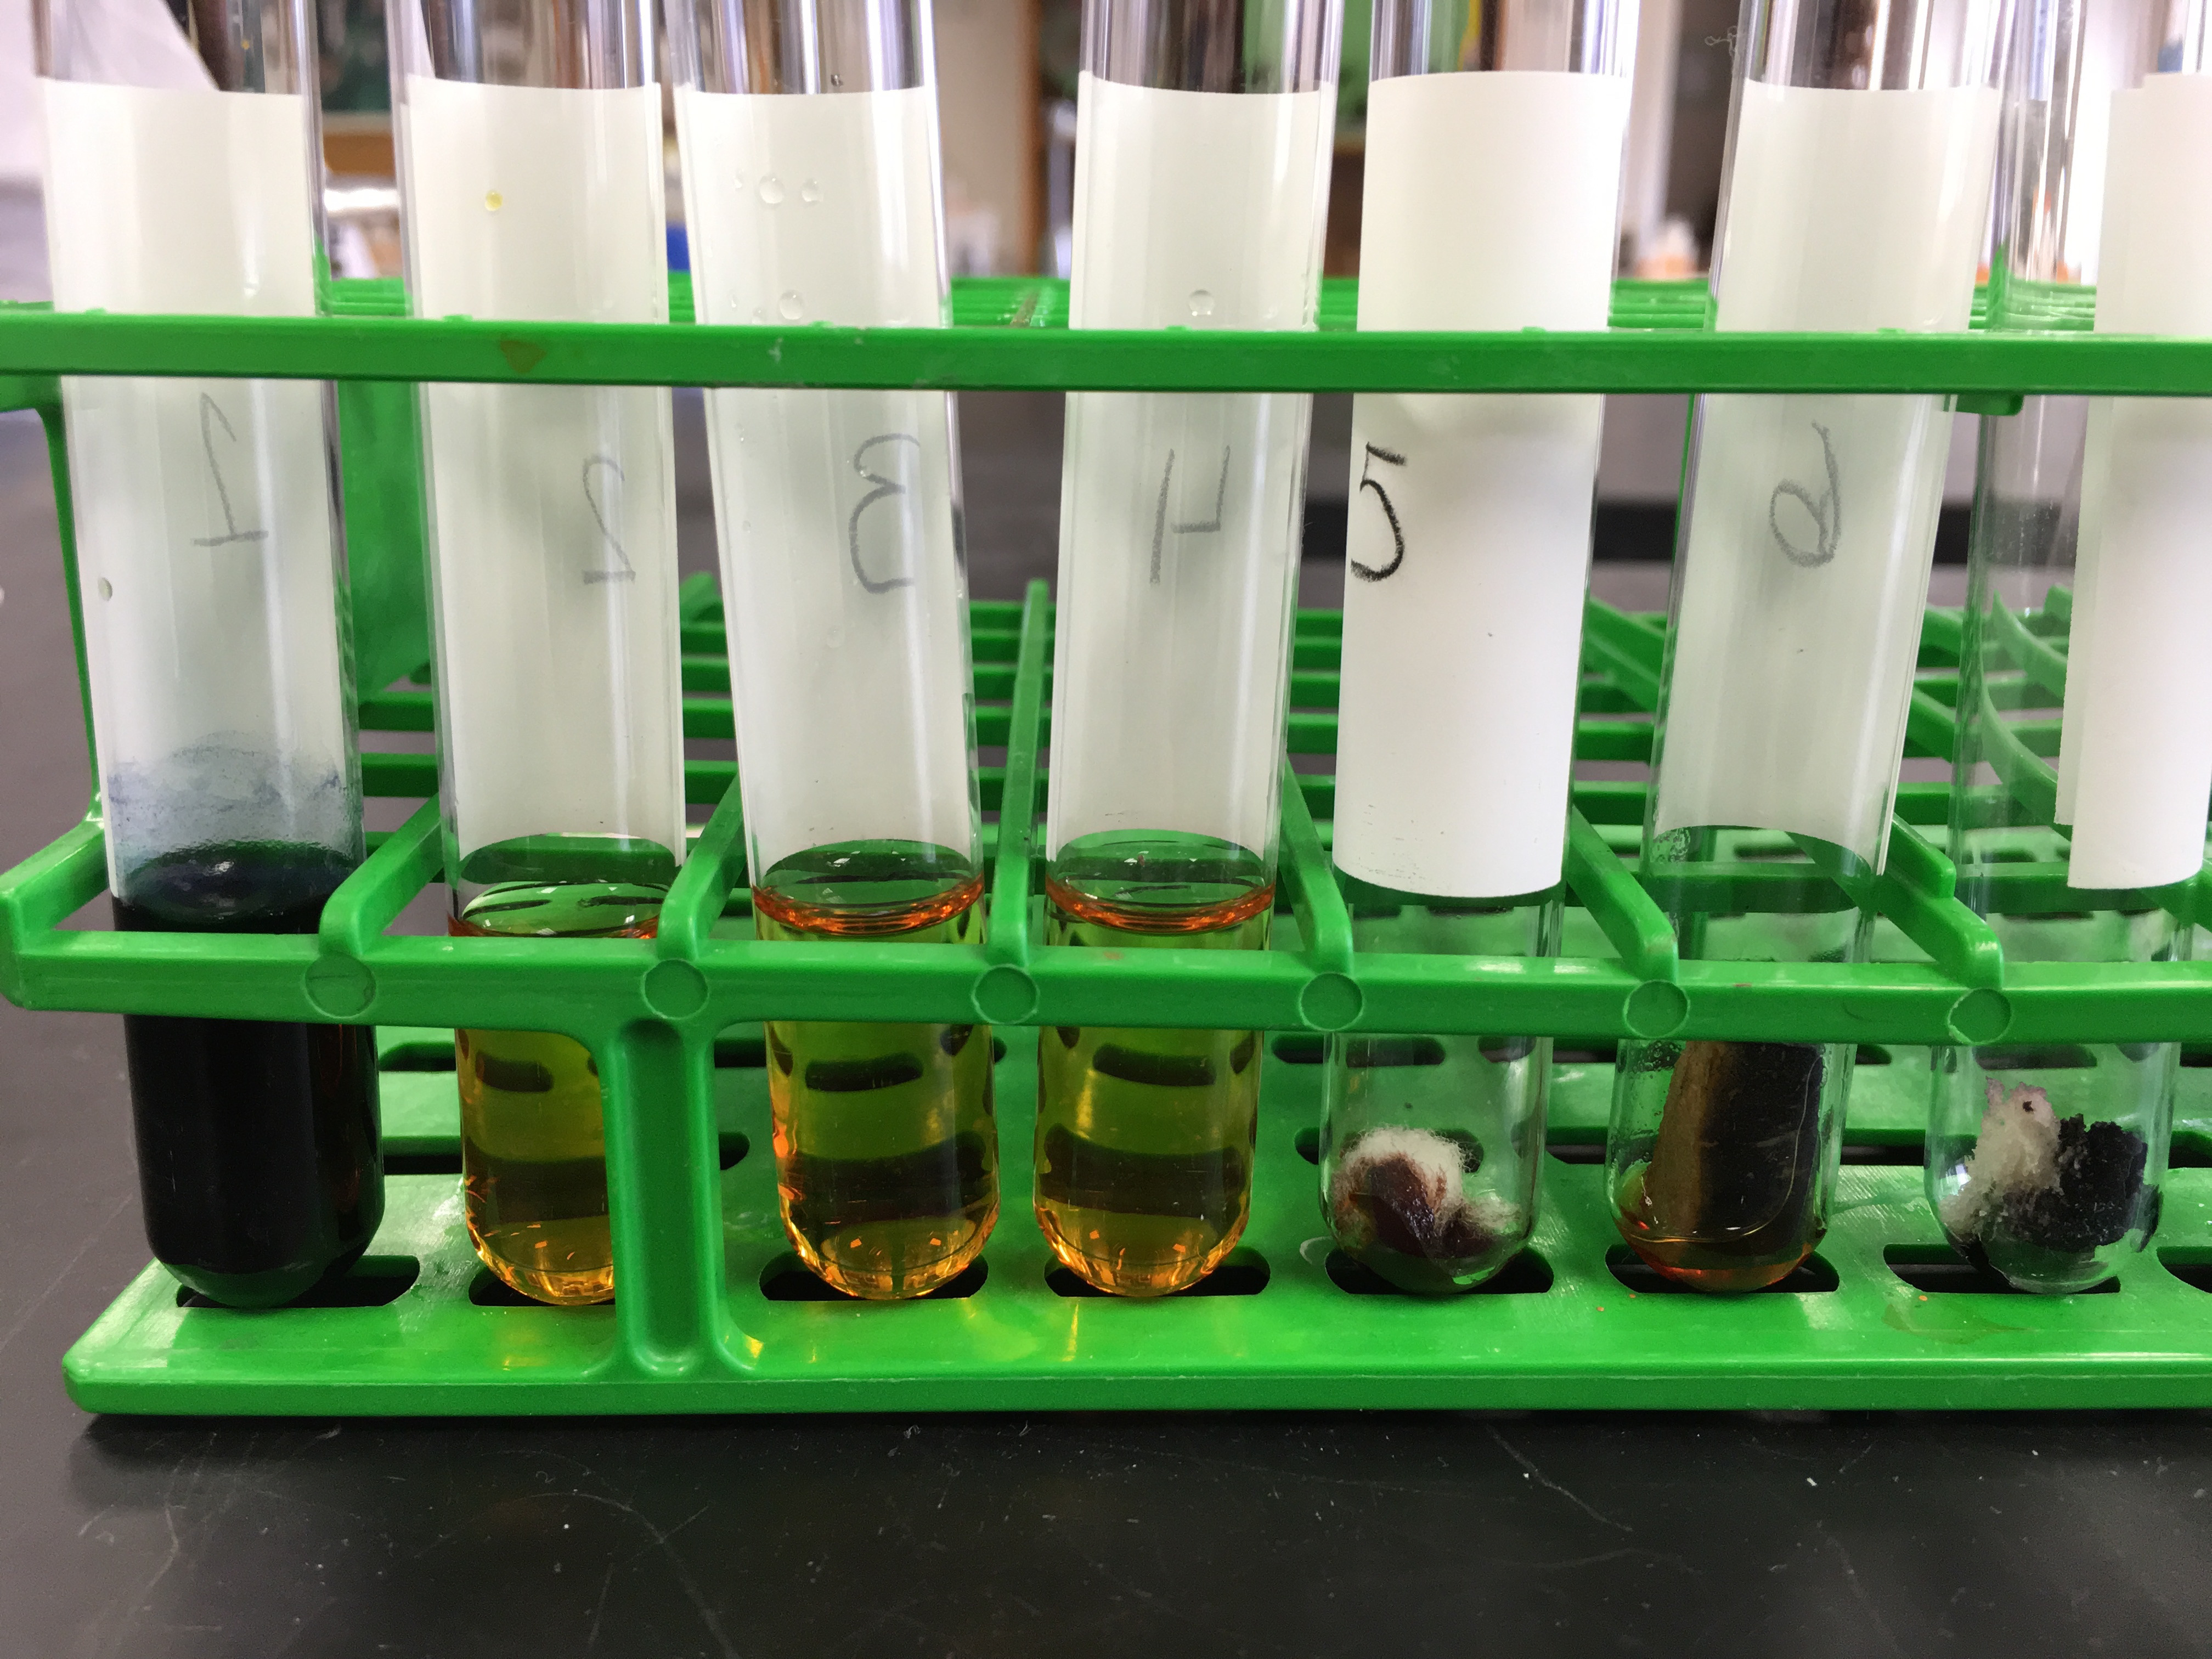
\includegraphics[width=0.7\linewidth]{./figures/chem_aspects/Results_exp_2} 

}

\caption{Results from experiment 2. Compare to your results!}\label{fig:exp2}
\end{figure}

\section{Test for Proteins}\label{test-for-proteins}

\href{https://en.wikipedia.org/wiki/Protein}{Proteins} are large
biomolecules, or macromolecules, consisting of one or more long chains
of amino acid residues. Proteins perform a vast array of functions
within organisms, including catalyzing metabolic reactions, DNA
replication, responding to stimuli, and transporting molecules from one
location to another. Proteins differ from one another primarily in their
sequence of amino acids, which is dictated by the nucleotide sequence of
their genes, and which usually results in protein folding into a
specific three-dimensional structure that determines its activity. A
linear chain of amino acid residues is called a polypeptide. A protein
contains at least one long polypeptide. Short polypeptides, containing
less than 20-30 residues, are rarely considered to be proteins and are
commonly called peptides, or sometimes oligopeptides. The individual
amino acid residues are bonded together by peptide bonds and adjacent
amino acid residues. The sequence of amino acid residues in a protein is
defined by the sequence of a gene, which is encoded in the genetic code.
In general, the genetic code specifies 20 standard amino acids; however,
in certain organisms the genetic code can include selenocysteine and-in
certain archaea-pyrrolysine.

The biuret test is a chemical test used for detecting the presence of
peptide bonds. In the presence of peptides, a copper(II) ion forms
violet-colored coordination complexes in an alkaline solution. The
biuret reaction can be used to assess the concentration of proteins
because peptide bonds occur with the same frequency per amino acid in
the peptide. The intensity of the color is directly proportional to the
protein concentration. Despite its name, the reagent does not in fact
contain biuret ((H\textsubscript{2}N-CO-)\textsubscript{2}NH). The test
is named so because it also gives a positive reaction to the
peptide-like bonds in the biuret molecule. In this assay, the copper(II)
binds with nitrogen present in the peptides of proteins. In a secondary
reaction, the copper(II) is reduced to copper(I). Due to its
insensitivity and little interference by free amino acids, this assay is
most useful for whole tissue samples and other sources with high protein
concentration.

\subsection{Experimental procedures}\label{experimental-procedures-3}

\begin{enumerate}
\def\labelenumi{\arabic{enumi}.}
\tightlist
\item
  Obtain 7 plastic test tubes and a test tube rack.
\item
  Using a wax pencil,label each tube with a number (1 to 7).
\item
  Place the tubes from left (tube \#1) to right (tube \#7) in the first
  row of a test tube rack.
\item
  Add the materials to these tubes as indicated in Table
  \ref{tab:protein} and mix well. No heating is needed to produce a
  reaction.
\item
  Wait 2 minutes and then record your observations in the table below.
  Base your conclusion only on the presence or absence of the violet
  color.
\end{enumerate}

\begin{longtable}[]{@{}clccc@{}}
\caption{\label{tab:protein} Test for protein.}\tabularnewline
\toprule
Tube \# & Test material & Biuret & Observation & Test\tabularnewline
\midrule
\endfirsthead
\toprule
Tube \# & Test material & Biuret & Observation & Test\tabularnewline
\midrule
\endhead
1 & 2 ml H\textsubscript{2}O & 2 ml & &\tabularnewline
2 & 2 ml sucrose & 2 ml & &\tabularnewline
3 & 2 ml albumin & 2 ml & &\tabularnewline
4 & 2 ml milk & 2 ml & &\tabularnewline
5 & a small piece of bread & 2 ml & &\tabularnewline
6 & 2 ml soy & 2 ml & &\tabularnewline
7 & 2 ml vegetable oil & 2 ml & &\tabularnewline
\bottomrule
\end{longtable}

\begin{figure}

{\centering 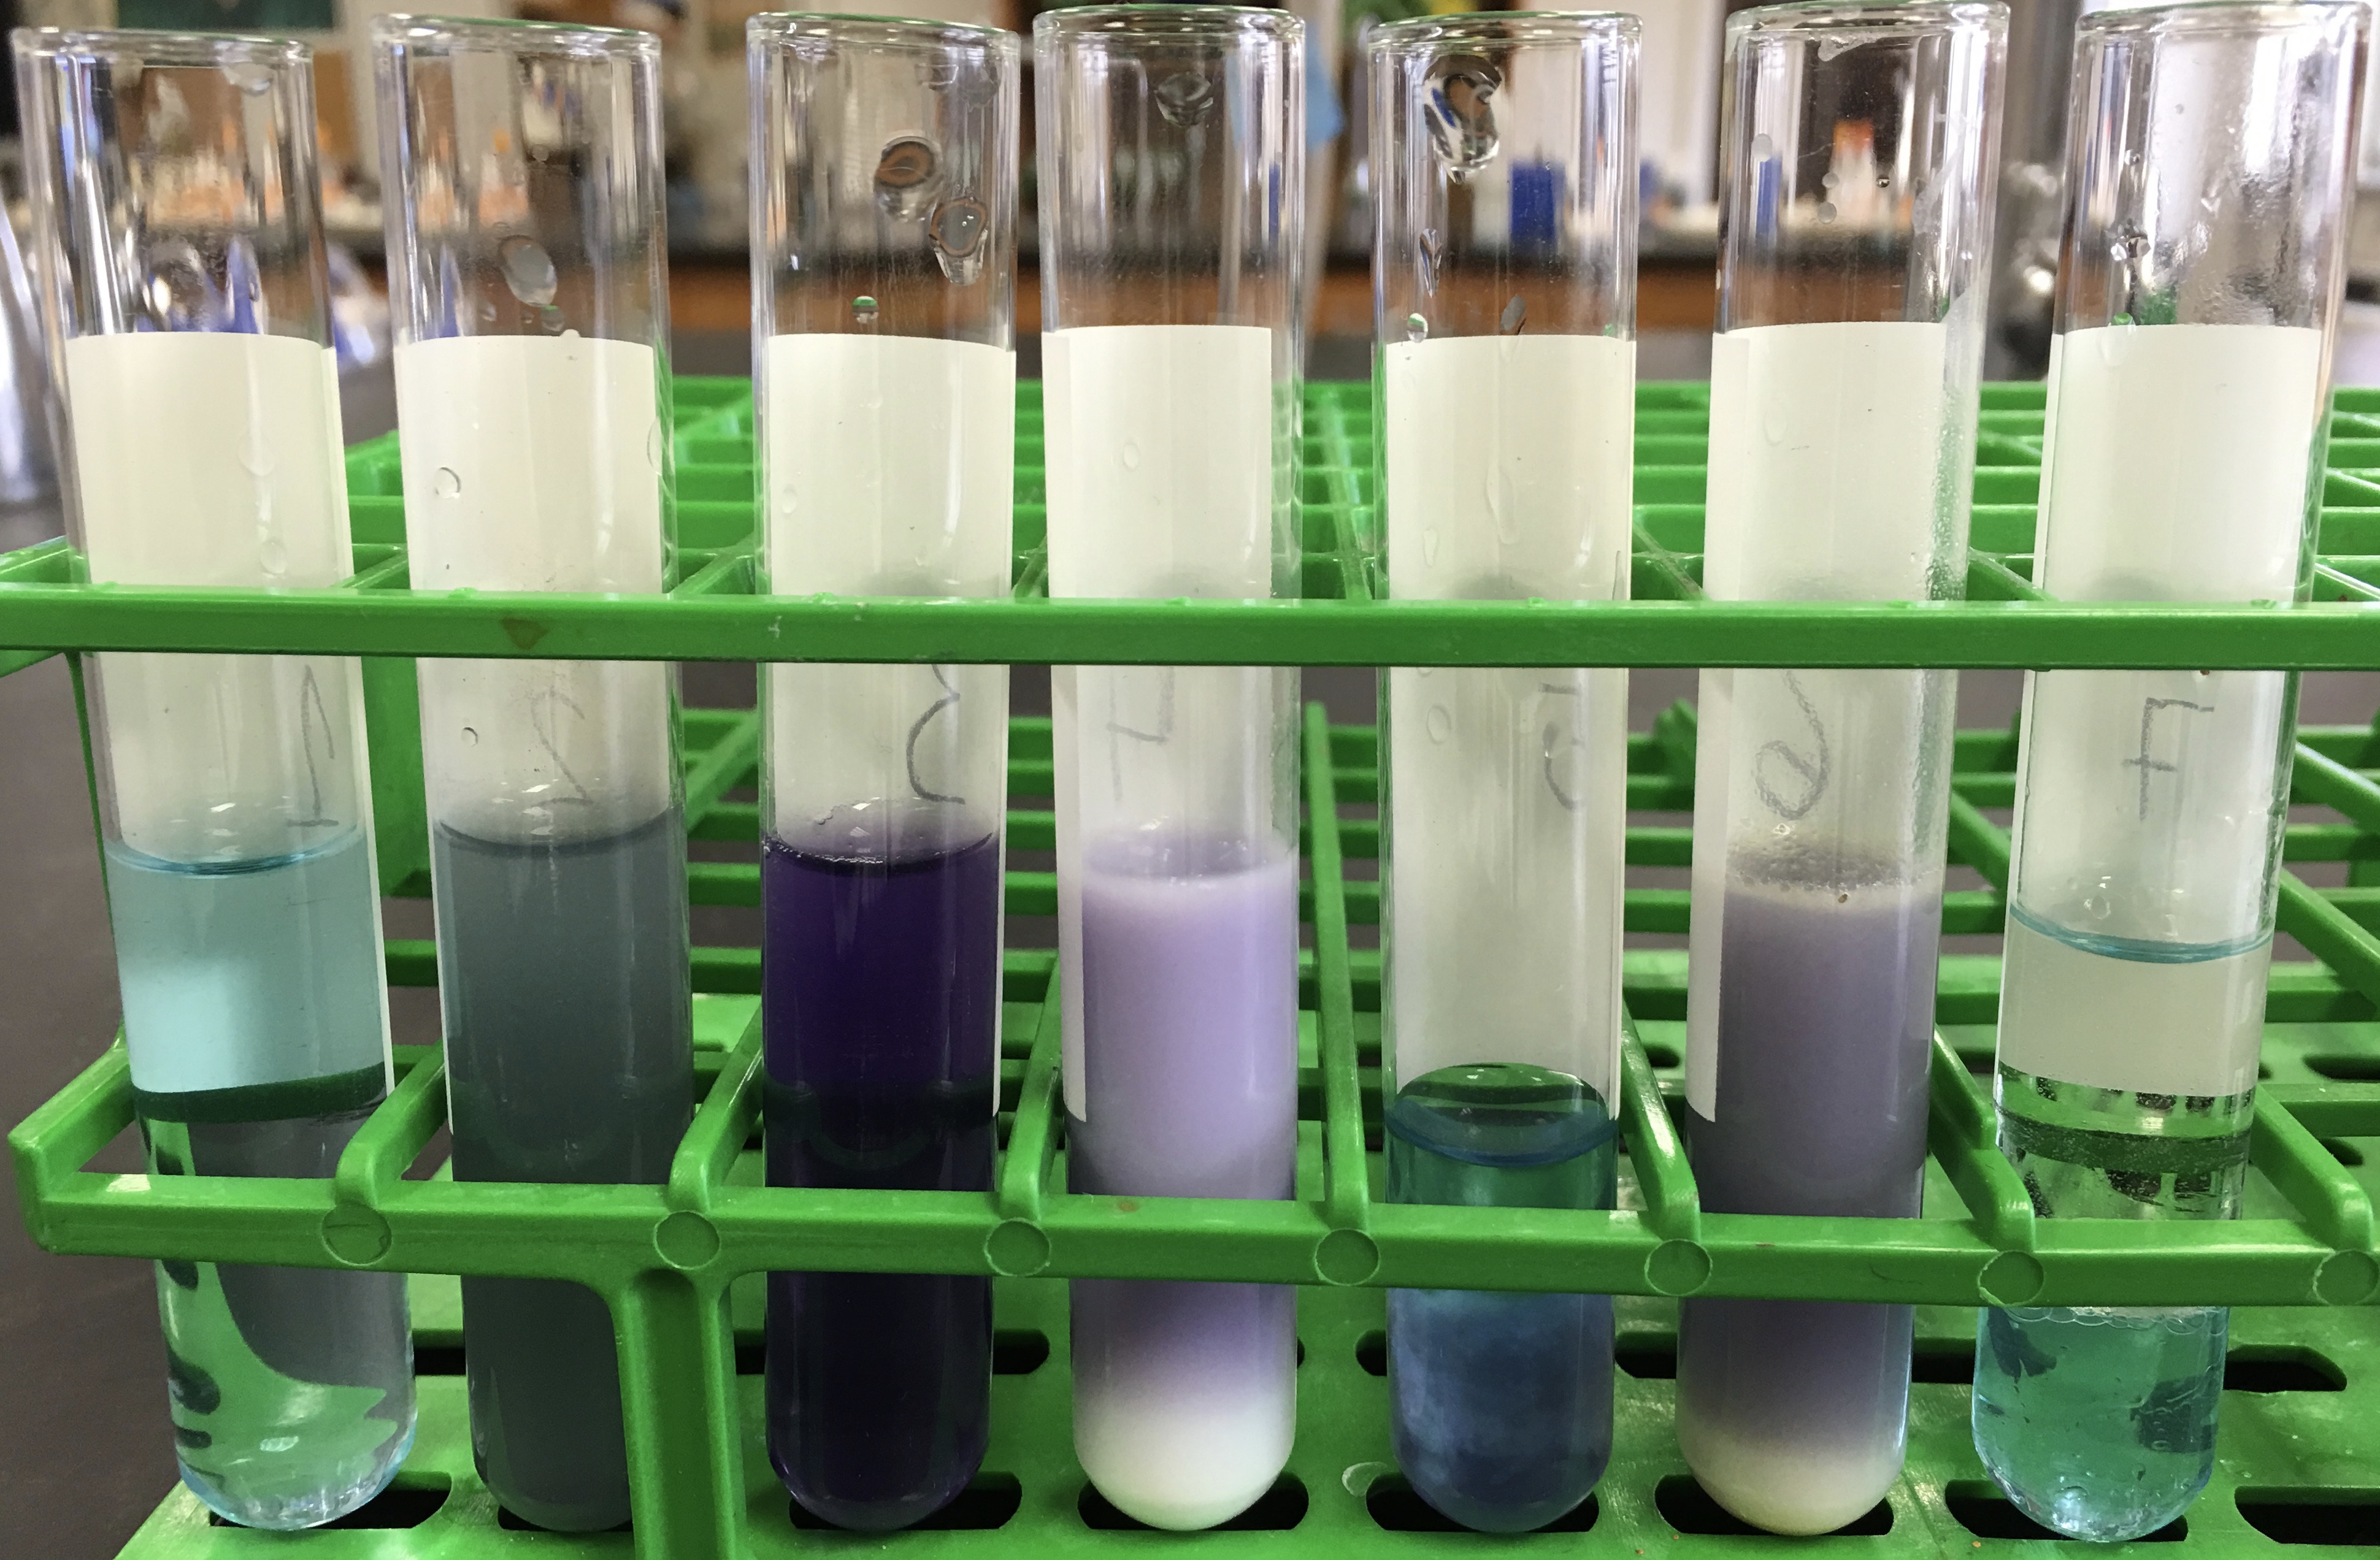
\includegraphics[width=0.7\linewidth]{./figures/chem_aspects/Results_exp_3} 

}

\caption{Results from experiment 3. Compare to your results!}\label{fig:exp3}
\end{figure}

\section{Cleaning up}\label{cleaning-up}

\begin{enumerate}
\def\labelenumi{\arabic{enumi}.}
\tightlist
\item
  Empty the contents of all plastic tubes into the labeled waste
  container (brown bottle) in the chemical fume hood.
\item
  Discard the empty tubes in the regular waste basket.
\end{enumerate}

\section{Test for Lipids}\label{test-for-lipids}

In biology, a \href{https://en.wikipedia.org/wiki/Lipid}{lipid} is a
substance of biological origin that is soluble in nonpolar solvents. It
comprises a group of naturally occurring molecules that include fats,
waxes, sterols, fat-soluble vitamins (such as vitamins A, D, E, and K),
monoglycerides, diglycerides, triglycerides, and phospholipids. The main
biological functions of lipids include storing energy, signaling, and
acting as structural components of cell membranes. Lipids have
applications in the cosmetic and food industries as well as in
nanotechnology. Scientists sometimes broadly define lipids as
hydrophobic or amphiphilic small molecules; the amphiphilic nature of
some lipids allows them to form structures such as vesicles, liposomes,
or membranes in an aqueous environment. Although the term ``lipid'' is
sometimes used as a synonym for fats, fats are a subgroup of lipids
called triglycerides. Lipids also encompass molecules such as fatty
acids and their derivatives (including tri-, di-, mono-glycerides, and
phospholipids), as well as other sterol-containing metabolites such as
cholesterol. Although humans and other mammals use various biosynthetic
pathways both to break down and to synthesize lipids, some essential
lipids cannot be made this way and must be obtained from the diet.

\subsection{Experimental procedures}\label{experimental-procedures-4}

\begin{enumerate}
\def\labelenumi{\arabic{enumi}.}
\tightlist
\item
  Obtain a small glass tube.
\item
  Add 2 ml of water into the glass tube.
\item
  Add 6 drops of vegetable oil to on top.
\item
  Shake thoroughly and observe the way the oil is dispersed only
  temporarily. This is an emulsion a mixture of two liquids, each
  insoluble in the other.
\item
  Now add 3 drops of lipid-specific red Sudan stain and mix again.
\item
  Add 2 ml of a liquid detergent to the tube and shake again.
\item
  Allow the tube to stand and note that the two phases (oil and water)
  are no longer distinctly separated. Detergent is often termed an
  emulsifier. Its molecules are water-soluble on one end and
  lipid-soluble on the other. These surround small oil droplets,
  water-soluble end out, and allow the droplets to stay suspended in the
  water.
\end{enumerate}

\section{Cleaning up}\label{cleaning-up-1}

Empty the contents of the glass tube into the labeled waste container
(brown bottle) in the chemical fume hood. Discard the glass tube in the
plastic container labeled ``broken glass'' in the chemical fume hood.

\section{Test for organic and inorganic compounds
(Demonstration)}\label{test-for-organic-and-inorganic-compounds-demonstration}

\subsection{Experimental procedures}\label{experimental-procedures-5}

\begin{enumerate}
\def\labelenumi{\arabic{enumi}.}
\tightlist
\item
  The instructor will use as Bunsen burner to heat a number of
  substances. Organic substances will burn, inorganic substances will
  remain unchanged.
\item
  Record your observation in Table \ref{tab:organic}.
\end{enumerate}

\begin{longtable}[]{@{}lcc@{}}
\caption{\label{tab:organic} Test for organic and inorganic
compounds.}\tabularnewline
\toprule
Substance & Organic & Inorganic\tabularnewline
\midrule
\endfirsthead
\toprule
Substance & Organic & Inorganic\tabularnewline
\midrule
\endhead
sugar & &\tabularnewline
table salt & &\tabularnewline
baking soda & &\tabularnewline
unknown & &\tabularnewline
\bottomrule
\end{longtable}

\section{Strawberry DNA extraction}\label{strawberry-dna-extraction}

We will use strawberries for
\href{https://en.wikipedia.org/wiki/DNA}{DNA} isolation. Wild
strawberries (Fragaria vesca) are ``diploid'' organisms (two sets of
chromosomes; 14 total), just like us, but the at a size of 240 million
base the strawberry genome (which has been fully sequenced) is much
smaller than ours (3 billion bases). The cultivated strawberry, Fragaria
ananassa, were generated only about 250 years ago are thus a very young
crop species. Botanically, it is neither a berry nor a true fruit.
Strawberry ``fruits'' consist of dry seeds that dot the surface of a
fleshy modified shoot tip (the receptacle). Genomically, Fragaria
ananassa is among the most complex of crop plants they harbor eight sets
of chromosomes (2n = 8x = 56), which are originally derived from as many
as four different diploid ancestors. Thus, \emph{Fragaria ananassa}, is
an octoploid organism, with 4 times more DNA in each cell than wild
strawberries. This property makes this fruit a great choice for
demonstrating DNA extraction. In addition, strawberries are soft and
easy to homogenize and ripe.

The first step of DNA extraction from live or dead cells is to lyse or
break open the cell. After the cells have broken open, a salt solution
such as sodium chloride (NaCl) and a detergent solution containing the
compound SDS (sodium dodecyl sulfate) is added. This solution breaks
down and emulsifies the fat \& proteins that make up the cell membrane.
Finally, ice cold ethanol is added. The alcohol and salt cause the DNA
to precipitate, or settle out of the solution, leaving behind all the
cellular components that aren't soluble in alcohol. The DNA can be
spooled (wound) on a stirring rod and pulled from the solution at this
point.

It is important to mention that the procedure for DNA extraction we are
using is really a procedure for total nucleic acid extraction. However,
much of the RNA extracted is cut by ribonucleases (enzymes that cut RNA)
that come in contact with the RNA when the cells are broken open.

\subsection{Experimental procedures}\label{experimental-procedures-6}

\begin{enumerate}
\def\labelenumi{\arabic{enumi}.}
\tightlist
\item
  Place 2 to 4 strawberries in a zip lock bag. Gently, mash up the fruit
  by pushing the bags with your hand against the lab bench. This will
  mechanically breakdown the cell wall.
\item
  Add 15 ml of the extraction buffer to the bag. Mix and mash again for
  one minute (chemical portion of the extraction procedure to lyse the
  cell membranes to release the DNA).
\item
  Filter the homogenate using cheesecloth. Hold the cheesecloth over the
  beaker with the help of a rubber band. This step removes cell
  organelles, broken cell walls, membrane fragments, and other cell
  debris.
\item
  Collect the filtrate; squeeze the cheesecloth to get the as much of
  the lysate as possible.
\item
  Pour the filtrate into a plastic tube. Fill the tube to about half the
  volume
\item
  Use the transfer pipet to drip alcohol slowly down the sides of the
  tube (about 5 ml of ice cold alcohol), while holding the tube at
  approximately an angle of 45 °. Try to make a clear and undisturbed
  layer of alcohol to float on the lysate. The line between the two
  layers is called the interface.
\item
  At the interface, you will see the DNA precipitate out of solution and
  float to the top. Spool the DNA on your glass rod.
\end{enumerate}

\section{Cleaning up}\label{cleaning-up-2}

\begin{enumerate}
\def\labelenumi{\arabic{enumi}.}
\tightlist
\item
  Empty the contents of the plastic tube into the labeled waste
  container (brown bottle) in the chemical fume hood.
\item
  Discard the empty tubes and other waste in the regular waste basket.
\item
  Rinse the glass rod and glassware with water and detergent.
\item
  Return the glass rod and glass ware to the trays on your bench where
  you originally found them.
\end{enumerate}

\section{Review Questions}\label{review-questions-1}

\begin{enumerate}
\def\labelenumi{\arabic{enumi}.}
\tightlist
\item
  What are organic compounds?
\item
  Which are the five most common elements in living organisms?
\item
  What are the four major groups of biomacromolecules?
\item
  What are the building blocks (monomers) of DNA?
\item
  What are lipids?
\item
  What are proteins?
\item
  What is a peptide bond?
\item
  What is chemical reduction?
\item
  What is chemical oxidation?
\item
  What are detergents?
\item
  Why do we use the detergent in the DNA extraction experiment?
\end{enumerate}

\chapter{Cell structure}\label{cell-structure}

The smallest unit of life is the
\href{https://en.wikipedia.org/wiki/Cell_(biology)}{cell}. In this lab,
we will look at eukaryotic (plant and animal) cells under the
microscope.

\begin{figure}

{\centering 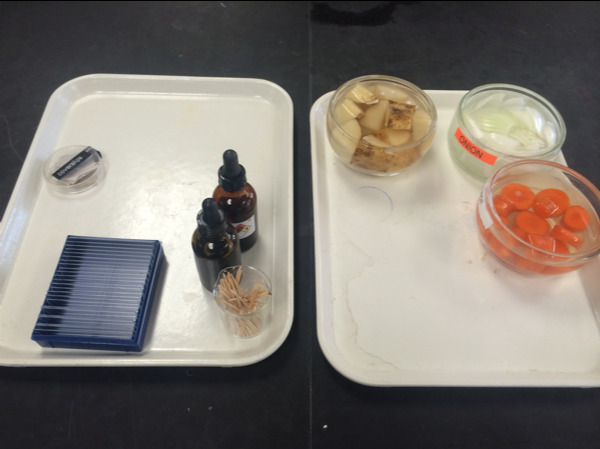
\includegraphics[width=0.7\linewidth]{./figures/cell_struc/materials} 

}

\caption{Experimemntal materials}\label{fig:materials}
\end{figure}

\section{Elodea cells}\label{elodea-cells}

\subsection{Experimental procedures}\label{experimental-procedures-7}

\begin{enumerate}
\def\labelenumi{\arabic{enumi}.}
\tightlist
\item
  Get a single leaf from the Elodea plant and mount it on a slide, cover
  it with a drop of water and a cover slip.
\item
  Look at the leaf under the microscope.
\item
  Notice that the cells are clearly delineated by the cell wall. Inside
  the cells are large oval-shaped green bodies, the chloroplasts.
\end{enumerate}

\section{Onion leaf epidermal cells}\label{onion-leaf-epidermal-cells}

\subsection{Experimental procedures}\label{experimental-procedures-8}

\begin{enumerate}
\def\labelenumi{\arabic{enumi}.}
\tightlist
\item
  Peel a very thin layer from the concave side of a piece of onion, and
  mount in water. Make sure the membrane lays very flat and is not
  wrinkled or folded on your slide.
\item
  Dim the light and find the nucleus, which is much easier to see here
  because there are no chloroplasts. Close examination should reveal one
  or more nucleoli in the nucleus.
\item
  Note the movement of small particles in the nearly trans- parent
  cytoplasm. This is Brownian movement, which we will study in more
  detail in another exercise.
\end{enumerate}

\section{Carrot root cells}\label{carrot-root-cells}

\subsection{Experimental procedures}\label{experimental-procedures-9}

\begin{enumerate}
\def\labelenumi{\arabic{enumi}.}
\tightlist
\item
  Use a razor blade and shave a very thin (almost translucent) slice of
  carrot onto a slide and prepare a wet mount of it.
\item
  Observe the orange-yellow bodies called chromoplasts, another type of
  plastid. Chromoplasts are enriched in pigments that give flowers,
  fruits, and fall leaves their colors, and carrots their orange color.
\end{enumerate}

\section{Potato cells}\label{potato-cells}

Potatoes are stems full of starch that is stored within the cells in
colorless plastids called amyloplasts.

\subsection{Experimental procedures}\label{experimental-procedures-10}

\begin{enumerate}
\def\labelenumi{\arabic{enumi}.}
\tightlist
\item
  Cut a very thin wedge-shaped sliver of potato.
\item
  Place it on a microscope slide.
\item
  Add a drop of iodine on top of the slice of potator.
\item
  Place a coverslip on top.
\item
  Observe the potato slice under the microscope.
\item
  Iodine stains starch a purple or blue-black color.
\end{enumerate}

\section{Cleaning up}\label{cleaning-up-3}

Discard the used glass slides in the container marked ``Broken glass''
in the fume hood.

\section{Human cheek cells}\label{human-cheek-cells}

The outer and inner surface of our body is formed by epithelial cells.

\subsection{Experimental procedures}\label{experimental-procedures-11}

\begin{enumerate}
\def\labelenumi{\arabic{enumi}.}
\tightlist
\item
  Rub the inner side of your cheek with a toothpick to pick up some
  cells.
\item
  Scrape the cloudy (cell-containing) fluid onto a slide, add a drop of
  dilute methylene blue, and observe under the microscope. Note that
  bacteria and possibly fungi on top and around your cheek cells.
\end{enumerate}

\section{Cleaning up}\label{cleaning-up-4}

Dispose of the toothpicks and the slide with the cheek cells in the
beakers containing (green looking) disinfectant liquid.

\section{Human blood cells}\label{human-blood-cells}

\href{https://en.wikipedia.org/wiki/Blood}{Blood} is a body fluid in
humans and other animals that delivers necessary substances such as
nutrients and oxygen to the cells and transports metabolic waste
products away from those same cells. In vertebrates, it is composed of
blood cells suspended in blood plasma. Plasma, which constitutes 55\% of
blood fluid, is mostly water (92\% by volume), and contains dissipated
proteins, glucose, mineral ions, hormones, carbon dioxide (plasma being
the main medium for excretory product transportation), and blood cells
themselves. Albumin is the main protein in plasma, and it functions to
regulate the colloidal osmotic pressure of blood. The blood cells are
mainly red blood cells (also called RBCs or erythrocytes), white blood
cells (also called WBCs or leukocytes) and platelets (also called
thrombocytes). The most abundant cells in vertebrate blood are red blood
cells. These contain hemoglobin, an iron-containing protein, which
facilitates oxygen transport by reversibly binding to this respiratory
gas and greatly increasing its solubility in blood. In contrast, carbon
dioxide is mostly transported extracellularly as bicarbonate ion
transported in plasma. Vertebrate blood is bright red when its
hemoglobin is oxygenated and dark red when it is deoxygenated. Some
animals, such as crustaceans and mollusks, use hemocyanin to carry
oxygen, instead of hemoglobin. Insects and some mollusks use a fluid
called hemolymph instead of blood, the difference being that hemolymph
is not contained in a closed circulatory system. In most insects, this
``blood'' does not contain oxygen-carrying molecules such as hemoglobin
because their bodies are small enough for their tracheal system to
suffice for supplying oxygen. Jawed vertebrates have an adaptive immune
system, based largely on white blood cells. White blood cells help to
resist infections and parasites. Platelets are important in the clotting
of blood. Blood is circulated around the body through blood vessels by
the pumping action of the heart. In animals with lungs, arterial blood
carries oxygen from inhaled air to the tissues of the body, and venous
blood carries carbon dioxide, a waste product of metabolism produced by
cells, from the tissues to the lungs to be exhaled.

\subsection{Experimental procedures}\label{experimental-procedures-12}

\begin{enumerate}
\def\labelenumi{\arabic{enumi}.}
\tightlist
\item
  Look at the prepared slide containing a human blood stain.
\item
  Can you distinguish multiple types of white blood cells?
\item
  Return the slide to the white slide box.
\end{enumerate}

\section{Review Questions}\label{review-questions-2}

\begin{enumerate}
\def\labelenumi{\arabic{enumi}.}
\tightlist
\item
  What the main structural features eukaryotic cells?
\item
  What distinguishes animal and plant cells?
\item
  What are mitochondria?
\item
  What are chloroplasts?
\end{enumerate}

\chapter{Exchange Between Cells and Their
Environment}\label{exchange-between-cells-and-their-environment}

\section{Diffusion}\label{diffusion}

\href{https://en.wikipedia.org/wiki/Diffusion}{Diffusion} is the net
movement of molecules or atoms from a region of high concentration (or
high chemical potential) to a region of low concentration (or low
chemical potential) as a result of random motion of the molecules or
atoms. The word diffusion derives from the Latin word, diffundere, which
means ``to spread way out''.

Diffusion is driven by a gradient in chemical potential of the diffusing
species. A gradient is the change in the value of a quantity
e.g.~concentration, pressure, or temperature with the change in another
variable, usually distance. A change in concentration over a distance is
called a concentration gradient, a change in pressure over a distance is
called a pressure gradient, and a change in temperature over a distance
is a called a temperature gradient.

A distinguishing feature of diffusion is that it depends on particle
random walk, and results in mixing or mass transport without requiring
directed bulk motion.

\section{Diffusion in air}\label{diffusion-in-air}

\subsection{Experimental procedures}\label{experimental-procedures-13}

\begin{enumerate}
\def\labelenumi{\arabic{enumi}.}
\tightlist
\item
  The instructor will open a bottle containing a fragrant substance.
\item
  Raise your hand when you smell the odor.
\end{enumerate}

\section{Diffusion in water}\label{diffusion-in-water}

\subsection{Experimental procedures}\label{experimental-procedures-14}

\begin{enumerate}
\def\labelenumi{\arabic{enumi}.}
\tightlist
\item
  Add 10 mL of water to a plastic test tube.
\item
  Drop a crystal of purple KMnO\textsubscript{4} (potassium
  permanganate) into it.
\item
  Put the tube in a test tube rack and place it where it will not be
  disturbed for the remainder of the lab period
\item
  From time to time, observe the how the KMnO\textsubscript{4} diffuses
  through the water.
\end{enumerate}

\section{Diffusion in a solid}\label{diffusion-in-a-solid}

\subsection{Experimental procedures}\label{experimental-procedures-15}

\begin{enumerate}
\def\labelenumi{\arabic{enumi}.}
\tightlist
\item
  Place a crystal of KMnO\textsubscript{4} onto a Petri dish with
  agarose gel.
\item
  Place a crystal of Malachite green about centimeters from the
  potassium permanganate crystal.
\item
  Note the rate of diffusion.
\item
  Find the molecular weights of each compound from
  \href{https://www.wikipedia.org}{Wikipedia}.
\end{enumerate}

\section{Diffusion Through a Selectively Permeable
Membrane}\label{diffusion-through-a-selectively-permeable-membrane}

A selectively permeable membrane is a type of biological or synthetic,
polymeric membrane that will allow certain molecules or ions to pass
through it by diffusion---or in the case of bioloigcal membranes
(e.g.~the cell membrane) by more specialized processes such as
facilitated diffusion and active transport. In this experiment we will
use a dialysis or
\href{https://en.wikipedia.org/wiki/Semipermeable_membranea}{semipermeable
membrane}--a selectively permeable membrane that allows particles below
a certain size through but excludes any particles that are larger.

\subsection{Experimental procedures}\label{experimental-procedures-16}

\begin{enumerate}
\def\labelenumi{\arabic{enumi}.}
\tightlist
\item
  Fill a 500-ml beaker with 300 ml of water.
\item
  Get a \textasciitilde{} 10 cm long piece of dialysis tubing and
  submerge it for \textasciitilde{} 10 seconds in the water.
\item
  Remove the dialysis tubing and clamp one end with the yellow clamp.
\item
  Rub the other end between the tips of your thumb and index fingers to
  open the dialysis membrane.
\item
  Get the starch solution and shake it well.
\item
  Fill the dialysis tubing with \textasciitilde{} 10 ml of starch
  solution.
\item
  Clamp off the open end.
\item
  Rinse with tap water.
\item
  Add iodine solution to the beaker with water until the solution
  becomes dark orange.
\item
  Add the dialysis tube containing the starch to the beaker and submerge
  completely in the water.
\item
  After about 15 minutes, observe the bag and surrounding liquid for any
  color change.
\item
  When starch molecules touch iodine, a blue or purplish color appears.
\item
  Start setting up Experiment 3 while you wait.
\end{enumerate}

\begin{figure}

{\centering 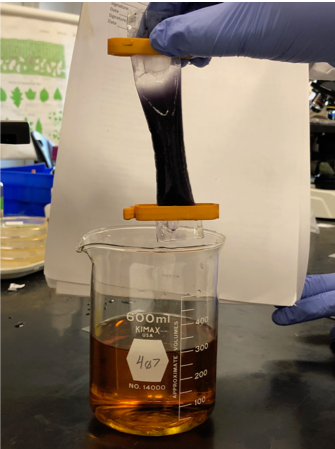
\includegraphics[width=0.7\linewidth]{./figures/exchange/Dialysis} 

}

\caption{Result of the dialysis experiment.}\label{fig:dialysis}
\end{figure}

\section{Brownian motion}\label{brownian-motion}

\href{https://en.wikipedia.org/wiki/Brownian_motion}{Brownian motion} is
the random motion of particles suspended in a fluid (a liquid or a gas)
resulting from their collision with the fast-moving molecules in the
fluid. This motion is named after
\href{https://en.wikipedia.org/wiki/Robert_Brown_(botanist,_born_1773)}{Robert
Brown} (botanist, born 1773). In 1827, while looking through a
microscope at particles trapped in cavities inside pollen grains in
water, he noted that the particles moved through the water; but he was
not able to determine the mechanisms that caused this motion. Atoms and
molecules had long been theorized as the constituents of matter, and
Albert Einstein published a paper in 1905 that explained in precise
detail how the motion that Brown had observed was a result of the pollen
being moved by individual water molecules, making one of his first big
contributions to science. This explanation of Brownian motion served as
convincing evidence that atoms and molecules exist and was further
verified experimentally by Jean Perrin in 1908. Perrin was awarded the
Nobel Prize in Physics in 1926 ``for his work on the discontinuous
structure of matter''. The direction of the force of atomic bombardment
is constantly changing, and at different times the particle is hit more
on one side than another, leading to the seemingly random nature of the
motion.

\subsection{Experimental procedures}\label{experimental-procedures-17}

\begin{enumerate}
\def\labelenumi{\arabic{enumi}.}
\tightlist
\item
  Put a drop of water on a microscope slide.
\item
  Take a toothpick and pick up a tiny bit of powdered carmine form the
  carmine container.
\item
  Hold the toothpick over the drop of water on the slide and tap it so
  that small specs of carmine fall into the water on the slide.
\item
  Add a coverslip on top of the drop of water with the carmine on the
  slide.
\item
  Put the slide under the microscope.
\item
  Observe the quivering motion of the particles under high power. A mass
  movement of particles in any one direction may result if the micro-
  scope is not quite level, or you are using only one stage clip, or the
  coverslip is caught under the stage clips. This is not what you are
  looking for.
\end{enumerate}

\section{Osmosis in Animal and Plant
Cells}\label{osmosis-in-animal-and-plant-cells}

\href{https://en.wikipedia.org/wiki/Osmosis}{Osmosis} is the spontaneous
net movement of solvent molecules through a selectively-permeable
membrane into a region of higher solute concentration, in the direction
that tends to equalize the solute concentrations on the two sides. A
selectively permeable membrane is a membrane that is permeable for some
but not other molecules. Osmotic pressure is defined as the external
pressure required to be applied so that there is no net movement of
solvent across the membrane. Osmotic pressure is a colligative property,
meaning that the osmotic pressure depends on the molar concentration of
the solute but not on its identity. Osmosis is a vital process in
biological systems, as biological membranes are selectively permeable.
In general, these membranes are impermeable to large and polar
molecules, such as ions, proteins, and polysaccharides, while being
permeable to non-polar or hydrophobic molecules like lipids as well as
to small molecules like oxygen, carbon dioxide, nitrogen, and nitric
oxide. Permeability depends on solubility, charge, or chemistry, as well
as solute size. Water molecules travel through the plasma membrane,
tonoplast membrane (vacuole) or protoplast by diffusing across the
phospholipid bilayer via aquaporins (small transmembrane proteins
similar to those responsible for facilitated diffusion and ion
channels). Osmosis provides the primary means by which water is
transported into and out of cells. The turgor pressure of a cell is
largely maintained by osmosis across the cell membrane between the cell
interior and its relatively hypotonic environment.

In unusual environments, osmosis can be very harmful to organisms. For
example, freshwater and saltwater aquarium fish placed in water of a
different salinity than that to which they are adapted to will die
quickly, and in the case of saltwater fish, dramatically. Another
example of a harmful osmotic effect is the use of table salt to kill
leeches and slugs. Suppose an animal or a cell is placed in a solution
of sugar or salt in water. 1. If the medium is hypotonic relative to the
cell cytoplasm - the cell will gain water through osmosis. 2. If the
medium is isotonic - there will be no net movement of water across the
cell membrane. 3. If the medium is hypertonic relative to the cell
cytoplasm - the cell will lose water by osmosis. Essentially, this means
that if a cell is put in a solution which has a solute concentration
higher than its own, it will shrivel, and if it is put in a solution
with a lower solute concentration than its own, the cell will swell and
may even burst.

\section{Crenation and Hemolysis of Red Blood
Cells}\label{crenation-and-hemolysis-of-red-blood-cells}

\href{https://en.wikipedia.org/wiki/Crenation}{Crenation} (Figure
\ref{fig:osmosisb}) is used to describe blood cells that look as if they
have projections extending from a smaller central area, like a spiked
ball. Hemolysis or haemolysis is the rupturing (lysis) of red blood
cells (erythrocytes) and the release of their contents (cytoplasm) into
surrounding fluid (e.g.~blood plasma).

(ref:osmosisb)
\href{https://commons.wikimedia.org/wiki/File:Osmotic_pressure_on_blood_cells_diagram.svg}{Osmosis
in red blood cells.}

\begin{figure}

{\centering 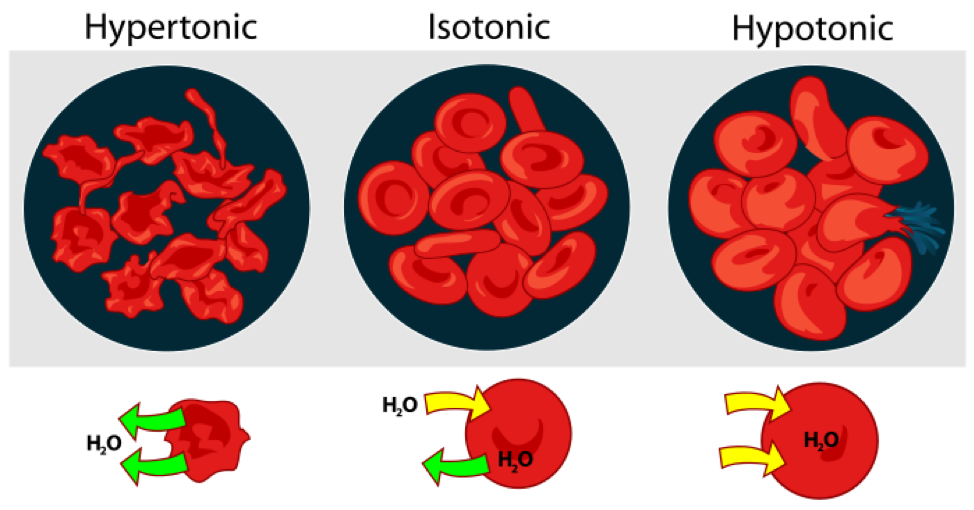
\includegraphics[width=0.7\linewidth]{./figures/exchange/Osmosis_blood} 

}

\caption{(ref:osmosisb)}\label{fig:osmosisb}
\end{figure}

\subsection{Experimental procedures}\label{experimental-procedures-18}

\begin{enumerate}
\def\labelenumi{\arabic{enumi}.}
\tightlist
\item
  Work in groups of three students
\item
  Get three clean slides.
\item
  With a wax pencil, mark the first slide ``5\%''``, the
  second''0.85\%``'', and the third ``0\%''" (distilled water).
\item
  Place a drop of the corresponding saline solution (NaCl) and distilled
  water on each slide using a plastic transfer pipette.
\item
  Add a small drop of sheep's blood beside the drop of saline.
\item
  Add a coverslip to each slide immediately, raising and lowering the
  coverslip a couple of times to mix the blood and saline.
\item
  Choose an area where the cells are thinly distributed and observe
  under 400x magnification. The differences are best compared if three
  microscopes are used at once, side by side.
\item
  Compare your observation with the figure shown above.
\end{enumerate}

\section{Turgor and Plasmolysis}\label{turgor-and-plasmolysis}

Osmotic pressure is the main cause of support in many plants. The
osmotic entry of water raises the turgor pressure exerted against the
cell wall, until it equals the osmotic pressure, creating a steady
state. When a plant cell is placed in a solution that is hypertonic
relative to the cytoplasm, water moves out of the cell and the cell
shrinks (Figure \ref{fig:osmosisp}). In doing so, the cell becomes
flaccid. In extreme cases, the cell becomes plasmolyzed - the cell
membrane disengages with the cell wall due to lack of water pressure on
it. When a plant cell is placed in a solution that is hypotonic relative
to the cytoplasm, water moves into the cell and the cell swells to
become turgid. Osmosis is responsible for the ability of plant roots to
draw water from the soil. Plants concentrate solutes in their root cells
by active transport, and water enters the roots by osmosis. Osmosis is
also responsible for controlling the movement of guard cells.

(ref:osmosisp)
\href{https://commons.wikimedia.org/wiki/File:Turgor_pressure_on_plant_cells_diagram.svg}{Osmosis
in plant cells.}

\begin{figure}

{\centering 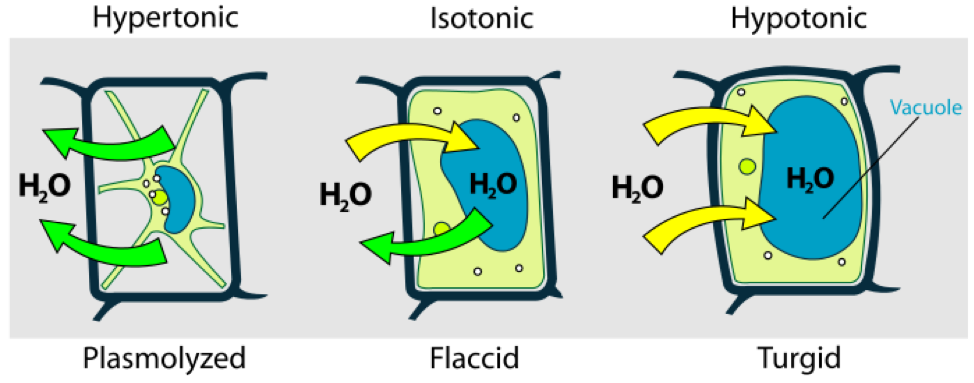
\includegraphics[width=0.7\linewidth]{./figures/exchange/Osmosis_plant} 

}

\caption{(ref:osmosisp)}\label{fig:osmosisp}
\end{figure}

\subsection{Experimental procedures}\label{experimental-procedures-19}

\begin{enumerate}
\def\labelenumi{\arabic{enumi}.}
\tightlist
\item
  Mount a leaf of Elodea in water on a slide and observe.
\item
  Blot off the water and add salt solution (7\% NaCl) by adding the salt
  at one side of the coverslip and drawing it under by using a paper
  towel to absorb the fluid from the opposite side of the coverslip.
\item
  Let it sit for a minute or two and observe again. The cell contains a
  vacuole, which holds most of the cell's water, similar to a water bag
  inside the cell. Note the clear space forming between the cell wall
  and the cell membrane.
\item
  Rinse the salt solution from the leaf and remount in water.
\item
  Observe periodically for about 5 minutes. How is the cell changing?
\end{enumerate}

\section{Review Questions}\label{review-questions-3}

\begin{enumerate}
\def\labelenumi{\arabic{enumi}.}
\tightlist
\item
  What is and what causes Brownian motion?
\item
  What is the definition of concentration?
\item
  What is a concentration gradient?
\item
  What is diffusion?
\item
  What is a selectively permeable membrane?
\item
  What is osmosis?
\item
  What is osmotic pressure?
\end{enumerate}

\chapter{Enzymes}\label{enzymes}

\href{https://en.wikipedia.org/wiki/Enzyme}{Enzymes} are macromolecular
biological catalysts. The molecules upon which enzymes may act are
called substrates and the enzyme converts the substrates into different
molecules known as products. Almost all metabolic processes in the cell
need enzyme catalysis in order to occur at rates fast enough to sustain
life. Metabolic pathways depend upon enzymes to catalyze individual
steps. Enzymes are known to catalyze more than 5,000 biochemical
reaction types. Most enzymes are proteins, although a few are catalytic
RNA molecules. The latter are called ribozymes. Enzymes' specificity
comes from their unique three-dimensional structures.

Like all catalysts, enzymes increase the reaction rate by lowering its
activation energy. Some enzymes can make their conversion of substrate
to product occur many millions of times faster. An extreme example is
orotidine 5'-phosphate decarboxylase, which allows a reaction that would
otherwise take millions of years to occur in milliseconds. Chemically,
enzymes are like any catalyst and are not consumed in chemical
reactions, nor do they alter the equilibrium of a reaction. Enzymes
differ from most other catalysts by being much more specific. Enzyme
activity can be affected by other molecules: inhibitors are molecules
that decrease enzyme activity, and activators are molecules that
increase activity. Many therapeutic drugs and poisons are enzyme
inhibitors. An enzyme's activity decreases markedly outside its optimal
temperature and pH.

Some enzymes are used commercially, for example, in the synthesis of
antibiotics. Some household products use enzymes to speed up chemical
reactions: enzymes in biological washing powders break down protein,
starch or fat stains on clothes, and enzymes in meat tenderizer break
down proteins into smaller molecules, making the meat easier to chew.

In this laboratory, we will study the effect of temperature,
concentration and pH and on the activity of the enzyme catalase.
Catalase speeds up the following reaction:

2 H\textsubscript{2}O\textsubscript{2} -\textgreater{} 2
H\textsubscript{2}O + O\textsubscript{2}

Hydrogen peroxide is toxic cells protect themselves. Cells therefore use
catalase to protect themselves. In these experiments, we will use
catalase enzyme from potato.

The first experiment will establish that our catalase works (positive
control) and that our reagents are not contaminated (negative control).

Hydrogen peroxide will not spontaneously degrade at room temperature in
the absence of enzyme. When catalase is added to hydrogen peroxide, the
reaction will take place and the oxygen produced will lead to the
formation of bubbles in the solution. The height of the bubbles above
the solution will be our measure of enzyme activity (Figure
\ref{fig:catalase}).

\begin{figure}

{\centering 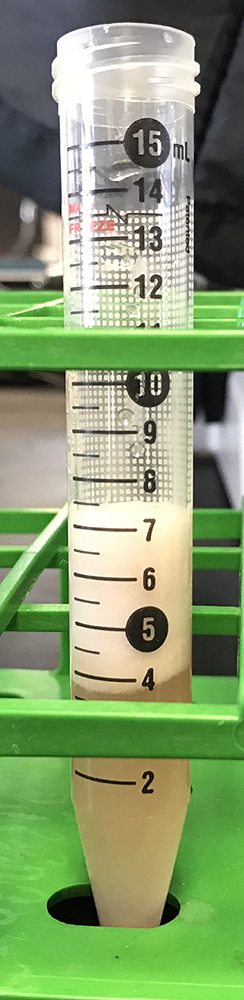
\includegraphics[width=0.7\linewidth]{./figures/enzymes/catalase} 

}

\caption{Catalase in action. Note the white bubbles above the darker liquid.}\label{fig:catalase}
\end{figure}

\section{Positive and negative controls (Experiment
1)}\label{positive-and-negative-controls-experiment-1}

\subsection{Experimental procedures}\label{experimental-procedures-20}

\begin{enumerate}
\def\labelenumi{\arabic{enumi}.}
\tightlist
\item
  Obtain and label three 15 ml conical plastic reaction tubes.
\item
  Then to \textbf{Tube 1}

  \begin{itemize}
  \tightlist
  \item
    Add 1 ml of potato juice (catalase) to tube 1 (use a plastic
    transfer pipette).
  \item
    Add 4 ml of hydrogen peroxide to tube 1. Swirl well to mix and wait
    at least 20 seconds for bubbling to develop.
  \item
    Use a ruler and measure the height of the bubble column above the
    liquid (in millimeters; use the centimeter scale of the ruler) and
    record the result in Table \ref{tab:control}.
  \end{itemize}
\item
  Then to \textbf{Tube 2}

  \begin{itemize}
  \tightlist
  \item
    Add 1 ml of water.
  \item
    Add 4 ml of hydrogen peroxide. Swirl well to mix and wait at least
    20 seconds.
  \item
    Measure the height of the bubble column (in millimeters) and record
    the result in Table \ref{tab:control}.
  \end{itemize}
\item
  Then to \textbf{Tube 3}

  \begin{itemize}
  \tightlist
  \item
    Add 1 ml of potato juice (catalase).
  \item
    Add 4 ml of sucrose solution. Swirl well to mix; wait 20 seconds.
  \item
    Measure the height of the bubble column and record the result in
    Table \ref{tab:control}.
  \end{itemize}
\end{enumerate}

\begin{longtable}[]{@{}cl@{}}
\caption{\label{tab:control} Positive and negative controls.}\tabularnewline
\toprule
Tube \# & Height of bubbles (mm)\tabularnewline
\midrule
\endfirsthead
\toprule
Tube \# & Height of bubbles (mm)\tabularnewline
\midrule
\endhead
1 &\tabularnewline
2 &\tabularnewline
3 &\tabularnewline
\bottomrule
\end{longtable}

\section{Effect of temperature on enzyme activity (Experiment
2)}\label{effect-of-temperature-on-enzyme-activity-experiment-2}

\subsection{Experimental procedures}\label{experimental-procedures-21}

\begin{enumerate}
\def\labelenumi{\arabic{enumi}.}
\tightlist
\item
  Obtain and label three tubes.
\item
  Add 1 ml of potato juice (catalase) to each tube.
\item
  Place tube 1 in the refrigerator, tube 2 in a 37 °C (Celsius) heat
  block, and tube 3 in a 97 °C heat block for 15 minutes.
\item
  Remove the tubes with the potato juice (catalase) from the
  refrigerator and heat blocks and immediately add 4 ml hydrogen
  peroxide to each tube.
\item
  Swirl well to mix and wait 20 seconds.
\item
  Measure the height of the bubble column (in millimeters) in each tube
  and record your observations in Table \ref{tab:temp}.
\end{enumerate}

\begin{longtable}[]{@{}cl@{}}
\caption{\label{tab:temp} Effect of temperature on enzyme
activity.}\tabularnewline
\toprule
Tube \# & Height of bubbles (mm)\tabularnewline
\midrule
\endfirsthead
\toprule
Tube \# & Height of bubbles (mm)\tabularnewline
\midrule
\endhead
1 &\tabularnewline
2 &\tabularnewline
3 &\tabularnewline
\bottomrule
\end{longtable}

\section{Effect of concentration on enzyme activity (Experiment
3)}\label{effect-of-concentration-on-enzyme-activity-experiment-3}

\subsection{Experimental procedures}\label{experimental-procedures-22}

\begin{enumerate}
\def\labelenumi{\arabic{enumi}.}
\tightlist
\item
  Obtain and label three tubes.
\item
  Then to \textbf{Tube 1}

  \begin{itemize}
  \tightlist
  \item
    Add 1 ml of water.
  \item
    Add 4 ml of hydrogen peroxide. Swirl well to mix and wait at least
    20 seconds.
  \item
    Measure the height of the bubble column (in millimeters) and record
    your observations in Table \ref{tab:concentration}.
  \end{itemize}
\item
  Then to \textbf{Tube 2}

  \begin{itemize}
  \tightlist
  \item
    Add 1 ml of potato juice (catalase).
  \item
    Add 4 ml of hydrogen peroxide. Swirl well to mix and wait at least
    20 seconds.
  \item
    Measure the height of the bubble column (in millimeters) and record
    your observations in Table \ref{tab:concentration}.
  \end{itemize}
\item
  Then to \textbf{Tube 3}

  \begin{itemize}
  \tightlist
  \item
    Add 3 ml of potato juice (catalase).
  \item
    Add 4 ml of hydrogen peroxide. Swirl well to mix and wait at least
    20 seconds.
  \item
    Measure the height of the bubble column (in millimeters) and record
    your observations in Table \ref{tab:concentration}.
  \end{itemize}
\end{enumerate}

\begin{longtable}[]{@{}cl@{}}
\caption{\label{tab:concentration} Effect of concentration on enzyme
activity.}\tabularnewline
\toprule
Tube \# & Height of bubbles (mm)\tabularnewline
\midrule
\endfirsthead
\toprule
Tube \# & Height of bubbles (mm)\tabularnewline
\midrule
\endhead
1 &\tabularnewline
2 &\tabularnewline
3 &\tabularnewline
\bottomrule
\end{longtable}

\section{Effect of pH on enzyme activity (Experiment
4)}\label{effect-of-ph-on-enzyme-activity-experiment-4}

\subsection{Experimental procedures}\label{experimental-procedures-23}

\begin{enumerate}
\def\labelenumi{\arabic{enumi}.}
\tightlist
\item
  Obtain 6 tubes and label each tube with a number from 1 to 6.
\item
  Place the tubes from left (tube \#1) to right (tube \#6) in the first
  row of a test tube rack.
\item
  Add to 1 ml of potato juice (catalase) to each tube.
\item
  Add 2 ml of water to tube 1.
\item
  Add 2 ml of pH buffer 3 to tube 2.
\item
  Add 2 ml of pH buffer 5 to tube 3.
\item
  Add 2 ml of pH buffer 7 to tube 4.
\item
  Add 2 ml of pH buffer 9 to tube 5.
\item
  Add 2 ml of pH buffer 12 to tube 6.
\item
  Add 4 ml of hydrogen peroxide to each of the six tubes.
\item
  Swirl each tube well to mix and wait at least 20 seconds.
\item
  Measure the height of the bubble column (in millimeters) in each tube
  and record your observations in Table \ref{tab:pH}.
\end{enumerate}

\begin{longtable}[]{@{}cl@{}}
\caption{\label{tab:pH} Effect of pH on enzyme activity.}\tabularnewline
\toprule
Tube \# & Height of bubbles (mm)\tabularnewline
\midrule
\endfirsthead
\toprule
Tube \# & Height of bubbles (mm)\tabularnewline
\midrule
\endhead
1 &\tabularnewline
2 &\tabularnewline
3 &\tabularnewline
4 &\tabularnewline
5 &\tabularnewline
6 &\tabularnewline
\bottomrule
\end{longtable}

\section{Cleaning up}\label{cleaning-up-5}

\begin{enumerate}
\def\labelenumi{\arabic{enumi}.}
\tightlist
\item
  Empty the contents of the plastic tubes into the labeled waste
  container (brown bottle) in the chemical fume hood.
\item
  Discard the empty tubes and other waste in the regular waste basket.
\item
  Rinse the glass rod and glassware with water and detergent.
\item
  Return the glass ware to the trays on your bench where you originally
  found them.
\end{enumerate}

\section{Review Questions}\label{review-questions-4}

\begin{enumerate}
\def\labelenumi{\arabic{enumi}.}
\tightlist
\item
  What is a catalyst?
\item
  What are enzymes?
\item
  What is the name of the enzyme that we studied in this laboratrory
  session?
\item
  What is an enzyme substrate?
\item
  What is the substrate of the enzyme that we used in this laborator
  seesion?
\item
  What are the products of the reachtion that was catalized by the
  enzyme that we studied in this laboratory seesion?
\item
  What is the active site of an enzyme?
\item
  What is the purpose of the negative and positive controls?
\item
  State the hypothesis that was tested in experiment 2?
\item
  State the hypothesis that was tested in experiment 3?
\item
  State the hypothesis that was tested in experiment 4?
\item
  The enzyme from potato appeared to work better at 4 °C than at 37 °C.
  Would you expect the same if we had used the equivalent human enzyme?
  Justify your answer.
\item
  Why did heating the enzyme at high heat (\textgreater{} 65 °C) result
  in loss of activity?
\end{enumerate}

\chapter{Photosynthesis}\label{photosynthesis}

In this lab, we will study the effect of light intensity and quality
(wave length - color) on
\href{https://en.wikipedia.org/wiki/Photosynthesis}{photosynthesis}. As
a measure of the rate of photosynthesis, we will monitor the rate of
oxygen production. When plants that spend their life submerged in water
release oxygen it forms bubbles, which we can count over a period of
time to determine photosynthesis rate.

Photosynthesis is a process used by plants and other organisms to
convert light energy into chemical energy that can later be released to
fuel the organisms' activities (energy transformation). This chemical
energy is stored in carbohydrate molecules, such as sugars, which are
synthesized from carbon dioxide and water - hence the name
photosynthesis, from the Greek phōs, ``light'', and synthesis, ``putting
together''. In most cases, oxygen is also released as a waste product.
Most plants, most algae, and cyanobacteria perform photosynthesis; such
organisms are called photoautotrophs. Photosynthesis is largely
responsible for producing and maintaining the oxygen content of the
Earth's atmosphere, and supplies all of the organic compounds and most
of the energy necessary for life on Earth.

Although photosynthesis is performed differently by different species,
the process always begins when energy from light is absorbed by proteins
called reaction centers that contain green chlorophyll pigments. In
plants, these proteins are held inside organelles called chloroplasts,
which are most abundant in leaf cells, while in bacteria they are
embedded in the plasma membrane. In these light-dependent reactions,
some energy is used to strip electrons from suitable substances, such as
water, producing oxygen gas. The hydrogen freed by the splitting of
water is used in the creation of two further compounds that act as an
immediate energy storage means: reduced nicotinamide adenine
dinucleotide phosphate (NADPH) and adenosine triphosphate (ATP), the
``energy currency'' of cells.

In plants, algae and cyanobacteria, long-term energy storage in the form
of sugars is produced by a subsequent sequence of light-independent
reactions called the Calvin cycle; some bacteria use different
mechanisms, such as the reverse Krebs cycle, to achieve the same end. In
the Calvin cycle, atmospheric carbon dioxide is incorporated into
already existing organic carbon compounds, such as ribulose bisphosphate
(RuBP). Using the ATP and NADPH produced by the light-dependent
reactions, the resulting compounds are then reduced and removed to form
further carbohydrates, such as glucose.

The first photosynthetic organisms probably evolved early in the
evolutionary history of life and most likely used reducing agents such
as hydrogen or hydrogen sulfide, rather than water, as sources of
electrons. Cyanobacteria appeared later; the excess oxygen they produced
contributed directly to the oxygenation of the Earth, which rendered the
evolution of complex life possible. Today, the average rate of energy
capture by photosynthesis globally is approximately 130 terawatts which
is about three times the current power consumption of human
civilization. Photosynthetic organisms also convert around 100-115
thousand million metric tons of carbon into biomass per year.

The main source of light on Earth is the Sun. Sunlight provides the
energy that green plants use to create sugars mostly in the form of
starches, which release energy into the living things that digest them.
This process of photosynthesis provides virtually all the energy used by
living things. The primary properties of visible light are intensity,
propagation direction, frequency or wavelength spectrum, and
polarization, while its speed in a vacuum, 299,792,458 meters per
second, is one of the fundamental constants of nature. Visible light, as
with all types of electromagnetic radiation (EMR), is experimentally
found to always move at this speed in a vacuum.

\section{Intensity of light}\label{intensity-of-light}

\href{https://en.wikipedia.org/wiki/Light}{Light} is electromagnetic
radiation within a certain portion of the electromagnetic spectrum
(Figure \ref{fig:spectrum}). The word usually refers to visible light,
which is visible to the human eye and is responsible for the sense of
sight. Visible light is usually defined as having wavelengths in the
range of 400-700 nanometres (nm), or 400 x 10\textsuperscript{-9} to 700
x 10\textsuperscript{-9} m, between the infrared (with longer
wavelengths) and the ultraviolet (with shorter wavelengths). This
wavelength means a frequency range of roughly 430-750 terahertz (THz).

(ref:spectrum)
\href{https://commons.wikimedia.org/wiki/File:Linear_visible_spectrum.svg}{Spectrum
of light. V, violet; B, blue; G, green Y, yellow; O, orange; R, red}

\begin{figure}

{\centering 
\includegraphics[width=0.7\linewidth]{./figures/photosynthesis/spectrum} 

}

\caption{(ref:spectrum)}\label{fig:spectrum}
\end{figure}

In this experiment (Figure \ref{fig:photosynthesis}), we will study the
effect of light intensity on the photosynthetic activity of \emph{Elodea
canadensis}. We will vary the light intensity by changing the distance
between the light source and the plant. We will count the emerging
oxygen bubbles as an indicator of the photosynthetic activity of the
plant.

\begin{figure}

{\centering 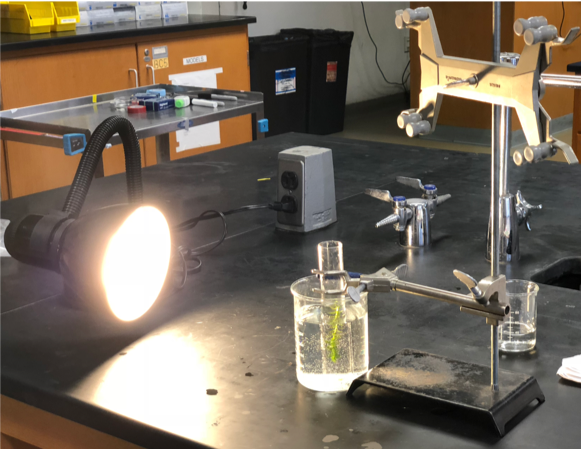
\includegraphics[width=0.7\linewidth]{./figures/photosynthesis/photosynthesis} 

}

\caption{Setup for photosynthesis experiment.}\label{fig:photosynthesis}
\end{figure}

\subsection{Experimental procedures}\label{experimental-procedures-24}

\begin{enumerate}
\def\labelenumi{\arabic{enumi}.}
\tightlist
\item
  Select a fresh, crisp sprig of Elodea about 15 cm in length.
\item
  While the plant is still submerged, cut 2-3 mm from its base.
\item
  Place the sprig upside down in a test tube filled with 0.25\% sodium
  bicarbonate. This is a buffer to absorb toxic materials evolved (i.e.,
  that are released. Keeping the plant submerged, position a light
  source 1 foot away and adjust so the light shines directly on the
  plant.
\item
  Place the test tube in a beaker of water as shown in Fig.
  \ref{fig:photosynthesis} to prevent overheating the plant. Allow the
  system to stand 7-10 minutes, or until bubbles begin to appear
  regularly.
\item
  Count the bubbles produced each minute for a 5-minute period and
  average them. Record your findings in the table.
\item
  Move the light back 2 feet from the plant, wait 5 minutes, and repeat
  counting. Record your findings in Table \ref{tab:intensity}.
\item
  Move the light back to 3 feet from the plant and repeat counting the
  bubbles.
\end{enumerate}

\begin{longtable}[]{@{}llllllc@{}}
\caption{\label{tab:intensity} Intensity of light.}\tabularnewline
\toprule
Distance of light source/Bubbles per minute & 1 & 2 & 3 & 4 & 5 &
Average\tabularnewline
\midrule
\endfirsthead
\toprule
Distance of light source/Bubbles per minute & 1 & 2 & 3 & 4 & 5 &
Average\tabularnewline
\midrule
\endhead
1 foot & & & & & &\tabularnewline
2 feet & & & & & &\tabularnewline
3 feet & & & & & &\tabularnewline
\bottomrule
\end{longtable}

\begin{figure}

{\centering 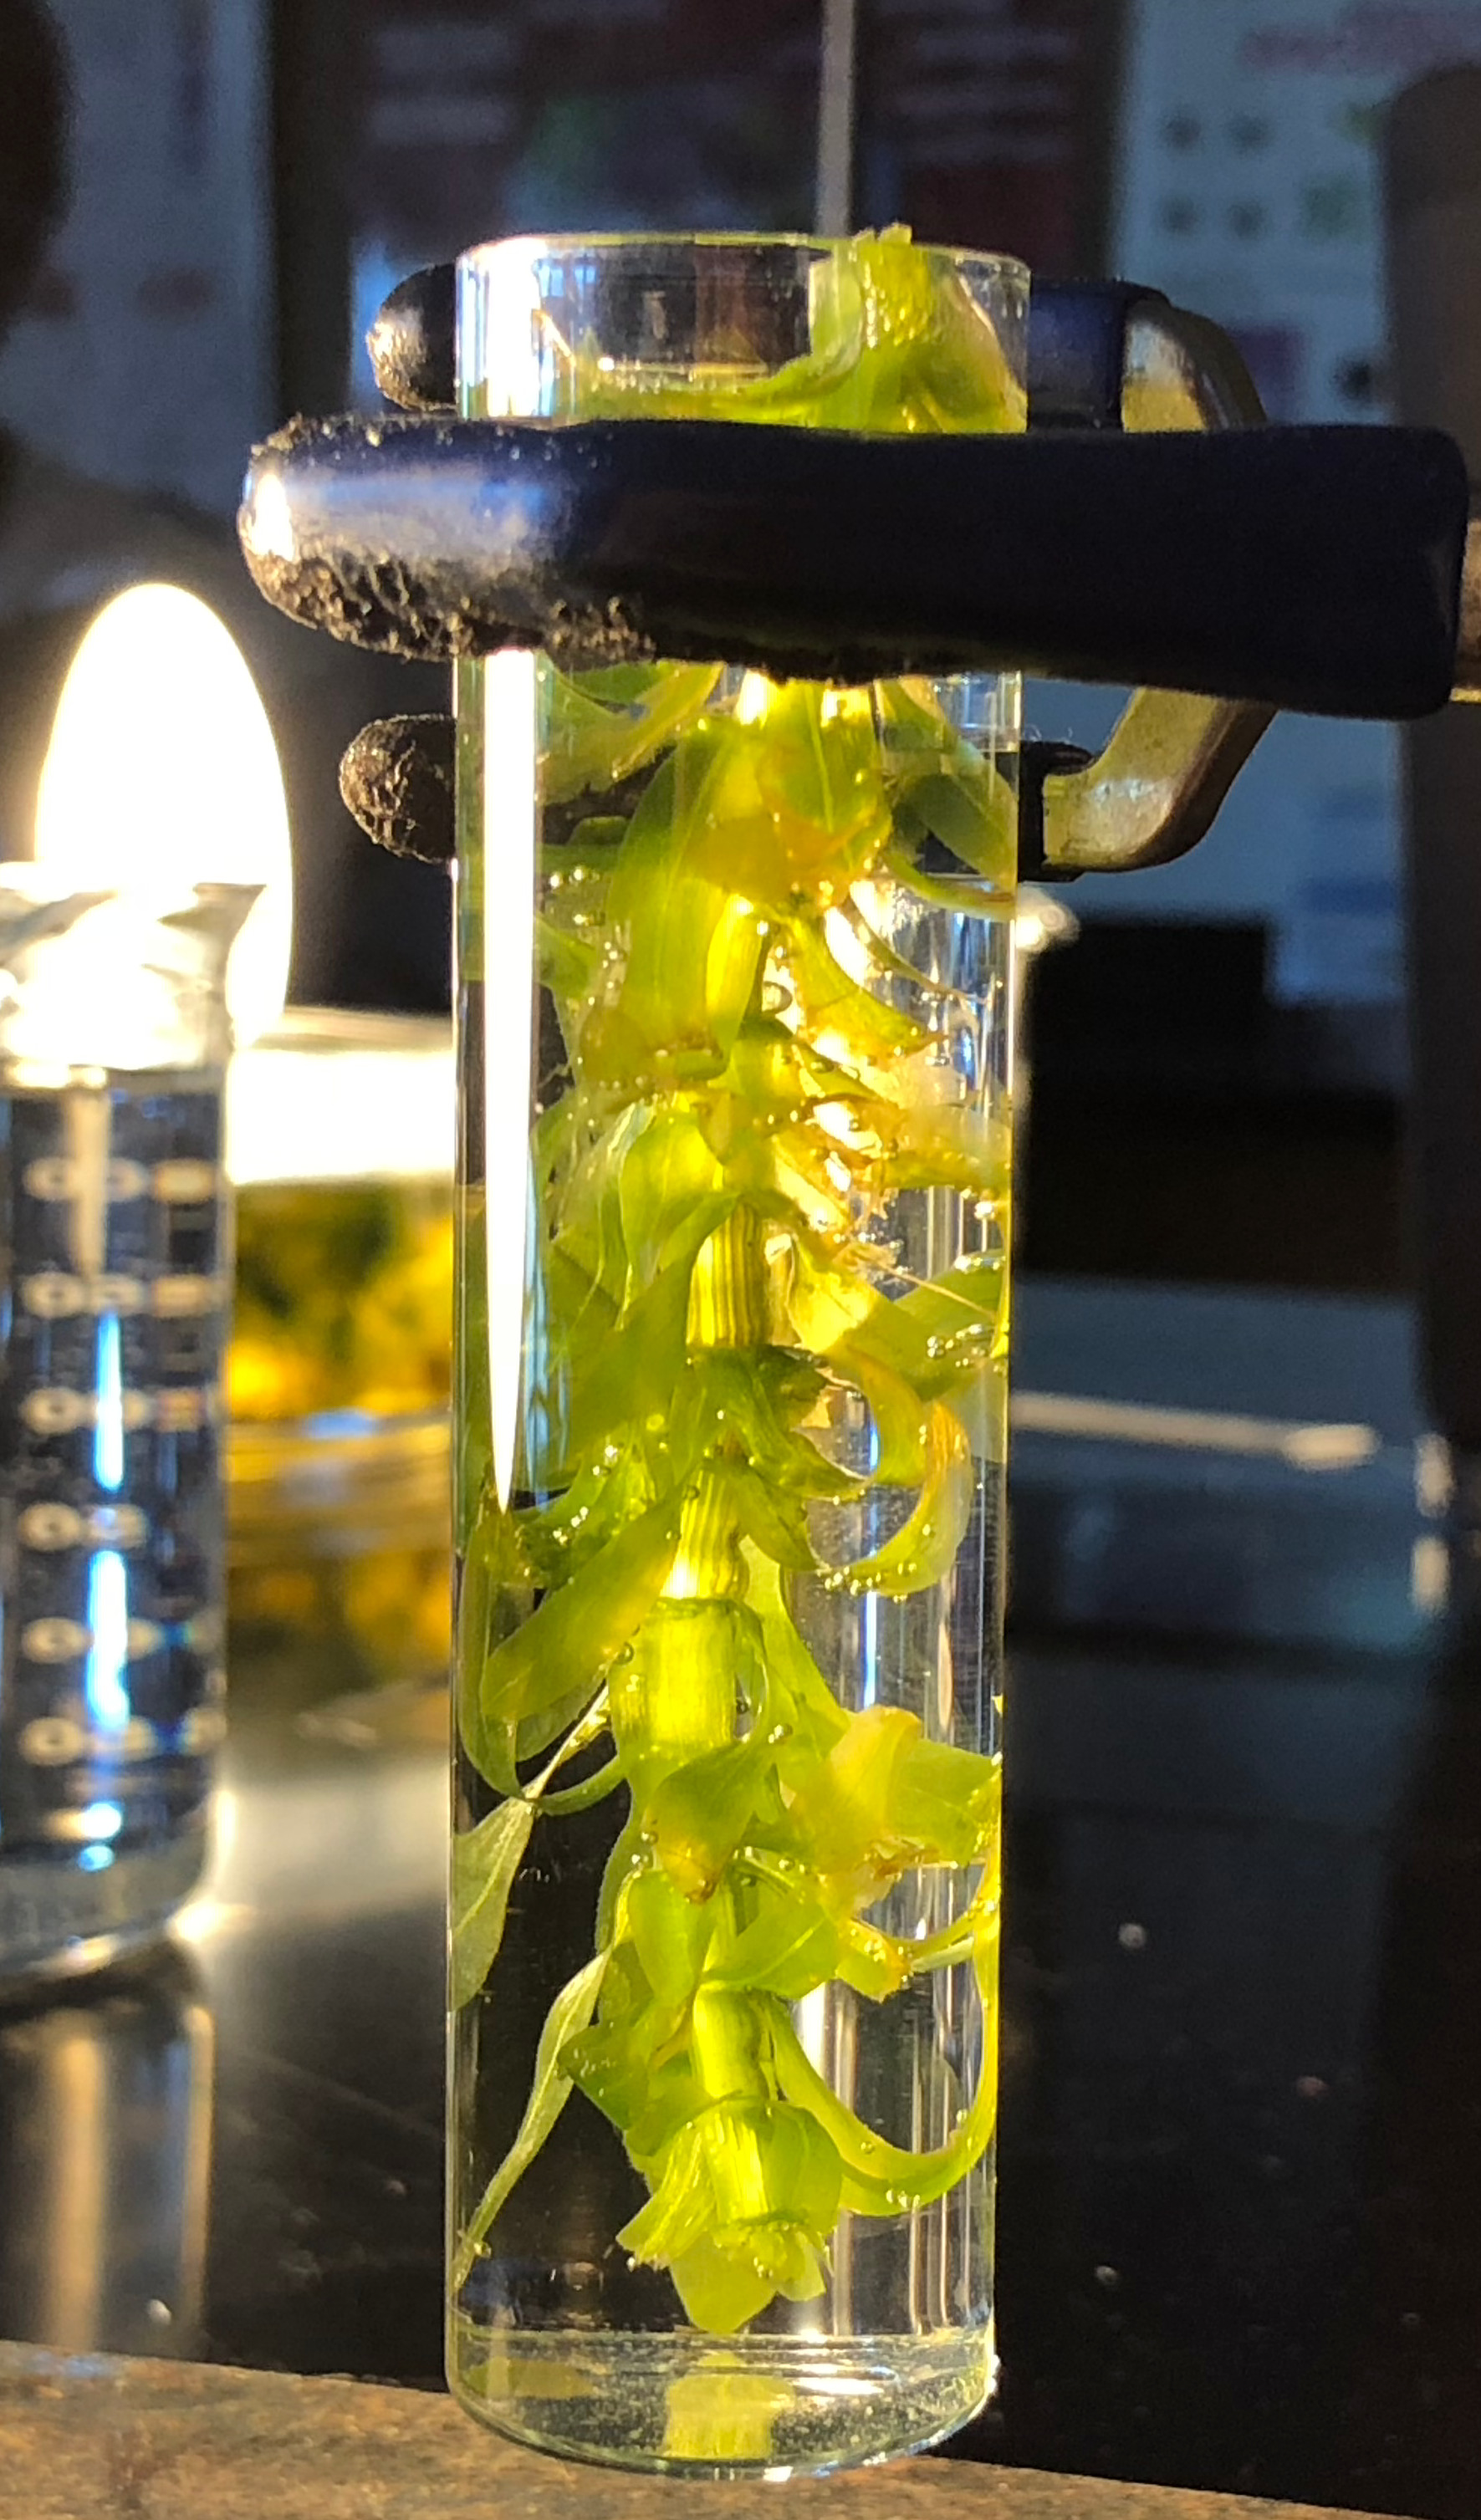
\includegraphics[width=0.7\linewidth]{./figures/photosynthesis/photosynthesis_bubbles} 

}

\caption{Appearance of bubbles indicates active photosynthesis.}\label{fig:bubbles}
\end{figure}

\section{Color of light}\label{color-of-light}

In this experiment, we will study the effect of the color of light on
the photosynthetic activity of \emph{Elodea canadensis}. We will use
filter to expose the plant to light of only a limited range of
wavelengths. We will again count the emerging oxygen bubbles as an
indicator of the photosynthetic activity of the plant.

\subsection{Experimental procedures}\label{experimental-procedures-25}

\begin{enumerate}
\def\labelenumi{\arabic{enumi}.}
\tightlist
\item
  Select a fresh, crisp sprig of Elodea about 15 cm in length.
\item
  While the plant is still submerged, cut 2-3 mm from its base.
\item
  Place the sprig upside down in a test tube filled with 0.25\% sodium
  bicarbonate. This is a buffer to absorb toxic materials evolved (i.e.,
  that are released). Keeping the plant submerged, position a light
  source 1 foot away and adjust so the light shines directly on the
  plant.
\item
  Place a colored filter between the test tube and the heat shield
  beaker and allow it to sit for 5 minutes.
\item
  Count bubbles for 5 minutes as in the previous experiment. Record your
  findings in Table \ref{tab:color}. Repeat steps 1 and 2 for each color
  filter available.
\end{enumerate}

\begin{longtable}[]{@{}llllllc@{}}
\caption{\label{tab:color} Color of light.}\tabularnewline
\toprule
Color of filter/Bubbles per minute & 1 & 2 & 3 & 4 & 5 &
Average\tabularnewline
\midrule
\endfirsthead
\toprule
Color of filter/Bubbles per minute & 1 & 2 & 3 & 4 & 5 &
Average\tabularnewline
\midrule
\endhead
blue & & & & & &\tabularnewline
orange & & & & & &\tabularnewline
red & & & & & &\tabularnewline
\bottomrule
\end{longtable}

\section{Determination of the light absorption spectrum of dye
solutions}\label{determination-of-the-light-absorption-spectrum-of-dye-solutions}

In this experiment, we will use a
\href{https://en.wikipedia.org/wiki/Spectrophotometry}{spectrophotometer}
to measure the differential absorption of light of different wavelength
by water stained with food dyes.

\begin{figure}

{\centering 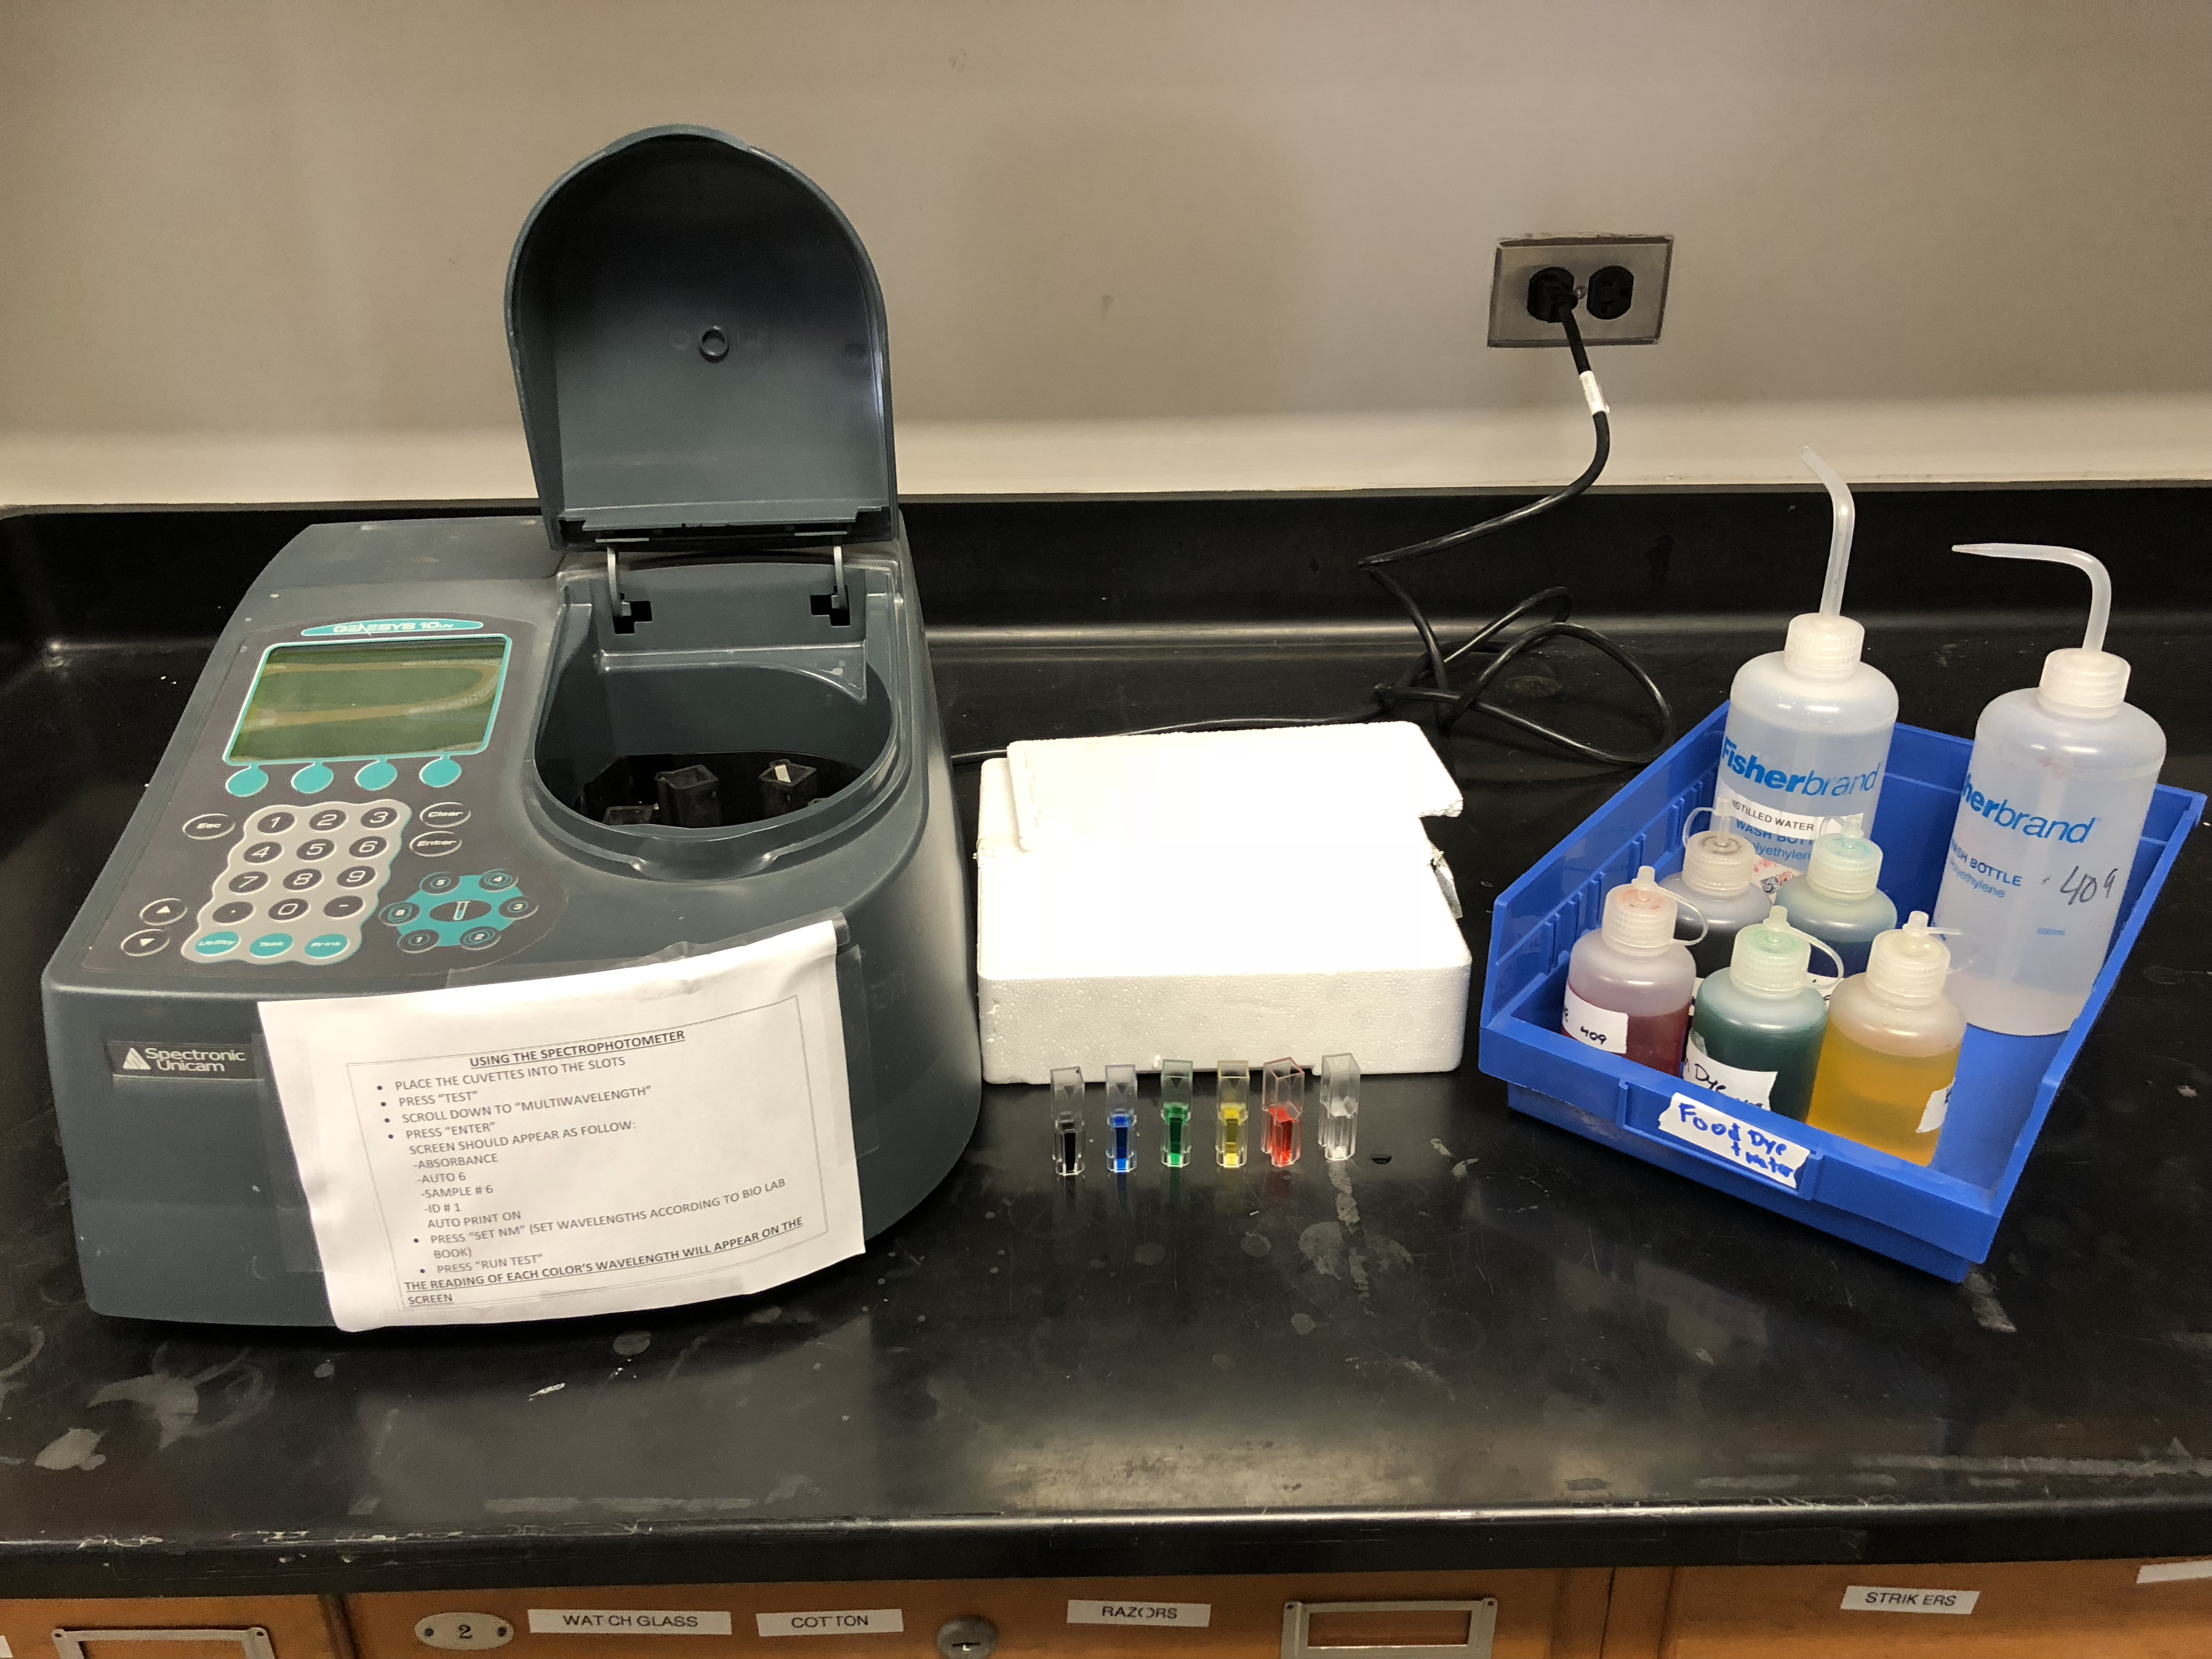
\includegraphics[width=0.7\linewidth]{./figures/photosynthesis/spectrophotometer} 

}

\caption{Spectrophotometer and cuvettes with dye solutions.}\label{fig:spectrophotometer}
\end{figure}

\subsection{Experimental procedures}\label{experimental-procedures-26}

\begin{enumerate}
\def\labelenumi{\arabic{enumi}.}
\tightlist
\item
  Take six cuvettes.
\item
  Fill one cuvette with water.
\item
  Fill each of the remaining five cuvettes with one of the color
  solutions listed in Table \ref{tab:absorption}.
\item
  Insert the cuvette with water into the slot marked ``B''.
\item
  Insert the other cuvettes into the slots marked 1 to 5 and write down
  which color is in which slot.
\item
  Following the instructions posted on the spectrophotometer, program
  the machine to take absorption measurements at wavelengths between
  380-740 nm in 20 nm steps.
\item
  Once the measurements are completed, write down the absorption number
  for each dye and wavelength.
\item
  Use a spreadsheet program to graph your results.
\item
  Compare your curves with the data shown in Figure
  \ref{fig:absorption}.
\end{enumerate}

\begin{figure}

{\centering 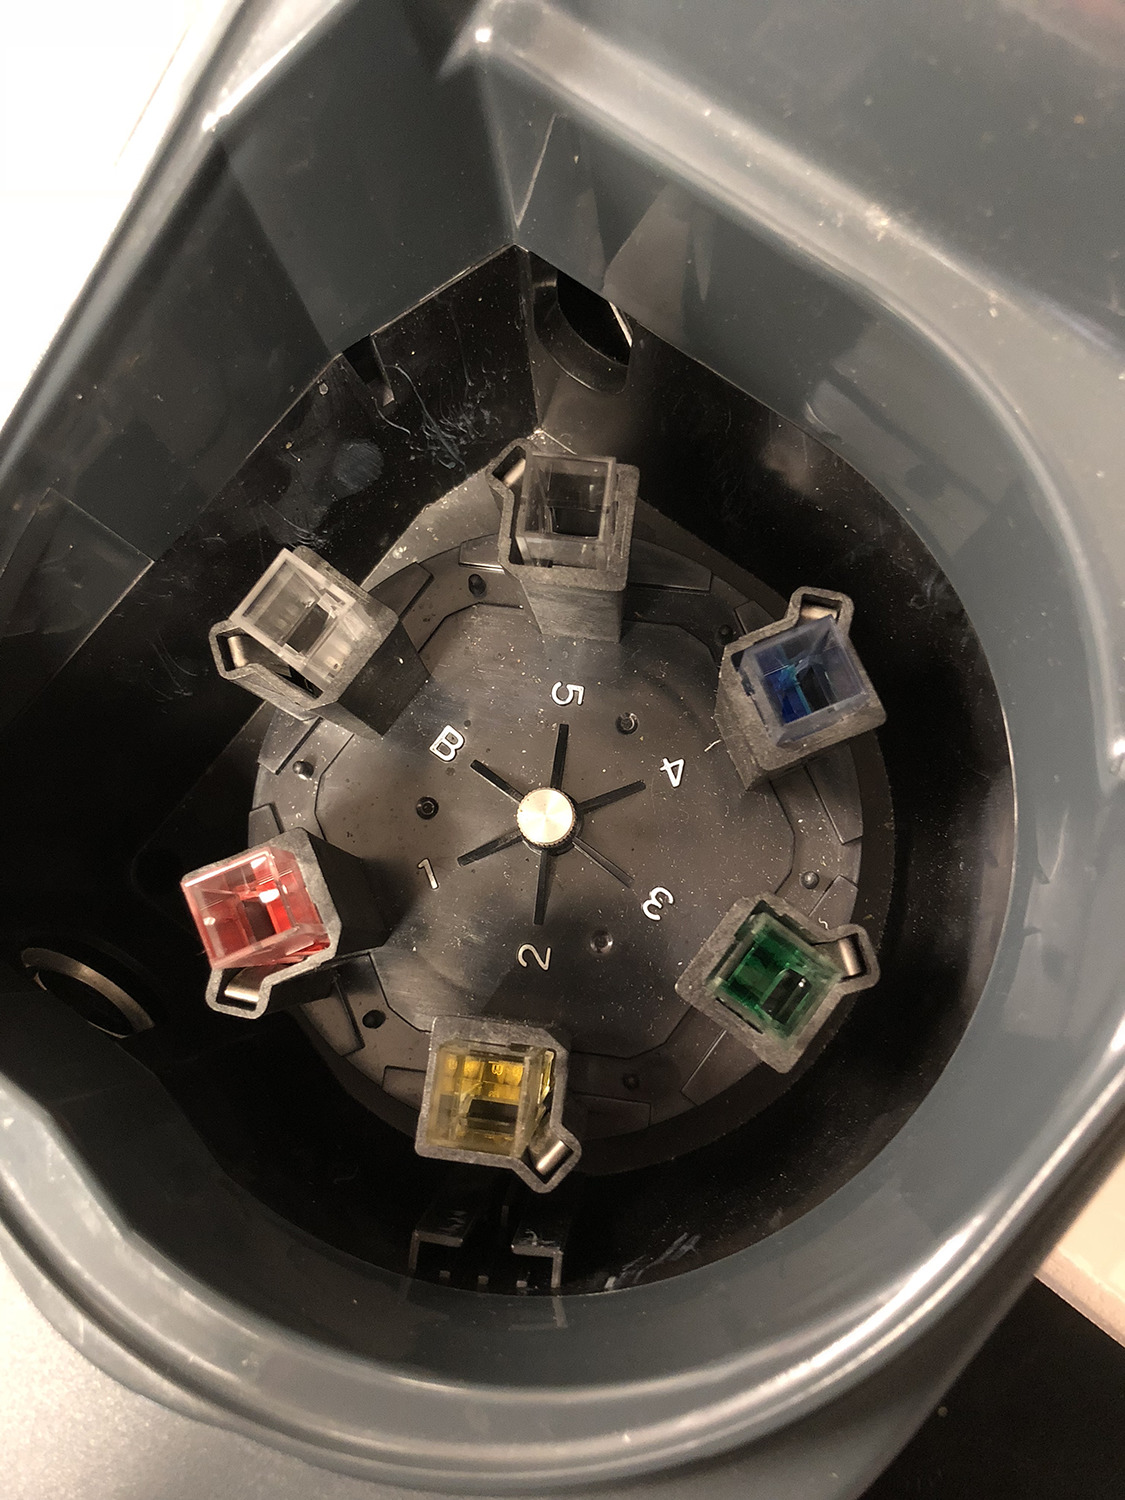
\includegraphics[width=0.7\linewidth]{./figures/photosynthesis/cuvettes} 

}

\caption{Cuvettes placed in the spectrophotometer.}\label{fig:cuvettes}
\end{figure}

\begin{longtable}[]{@{}clllll@{}}
\caption{\label{tab:absorption} Determination of the light absorption
spectrum of dye solutions.}\tabularnewline
\toprule
Wavelength (nm) & Purple & Blue & Green & Yellow & Red\tabularnewline
\midrule
\endfirsthead
\toprule
Wavelength (nm) & Purple & Blue & Green & Yellow & Red\tabularnewline
\midrule
\endhead
380 & & & & &\tabularnewline
400 & & & & &\tabularnewline
420 & & & & &\tabularnewline
\ldots{} & & & & &\tabularnewline
720 & & & & &\tabularnewline
740 & & & & &\tabularnewline
\bottomrule
\end{longtable}

\begin{figure}

{\centering 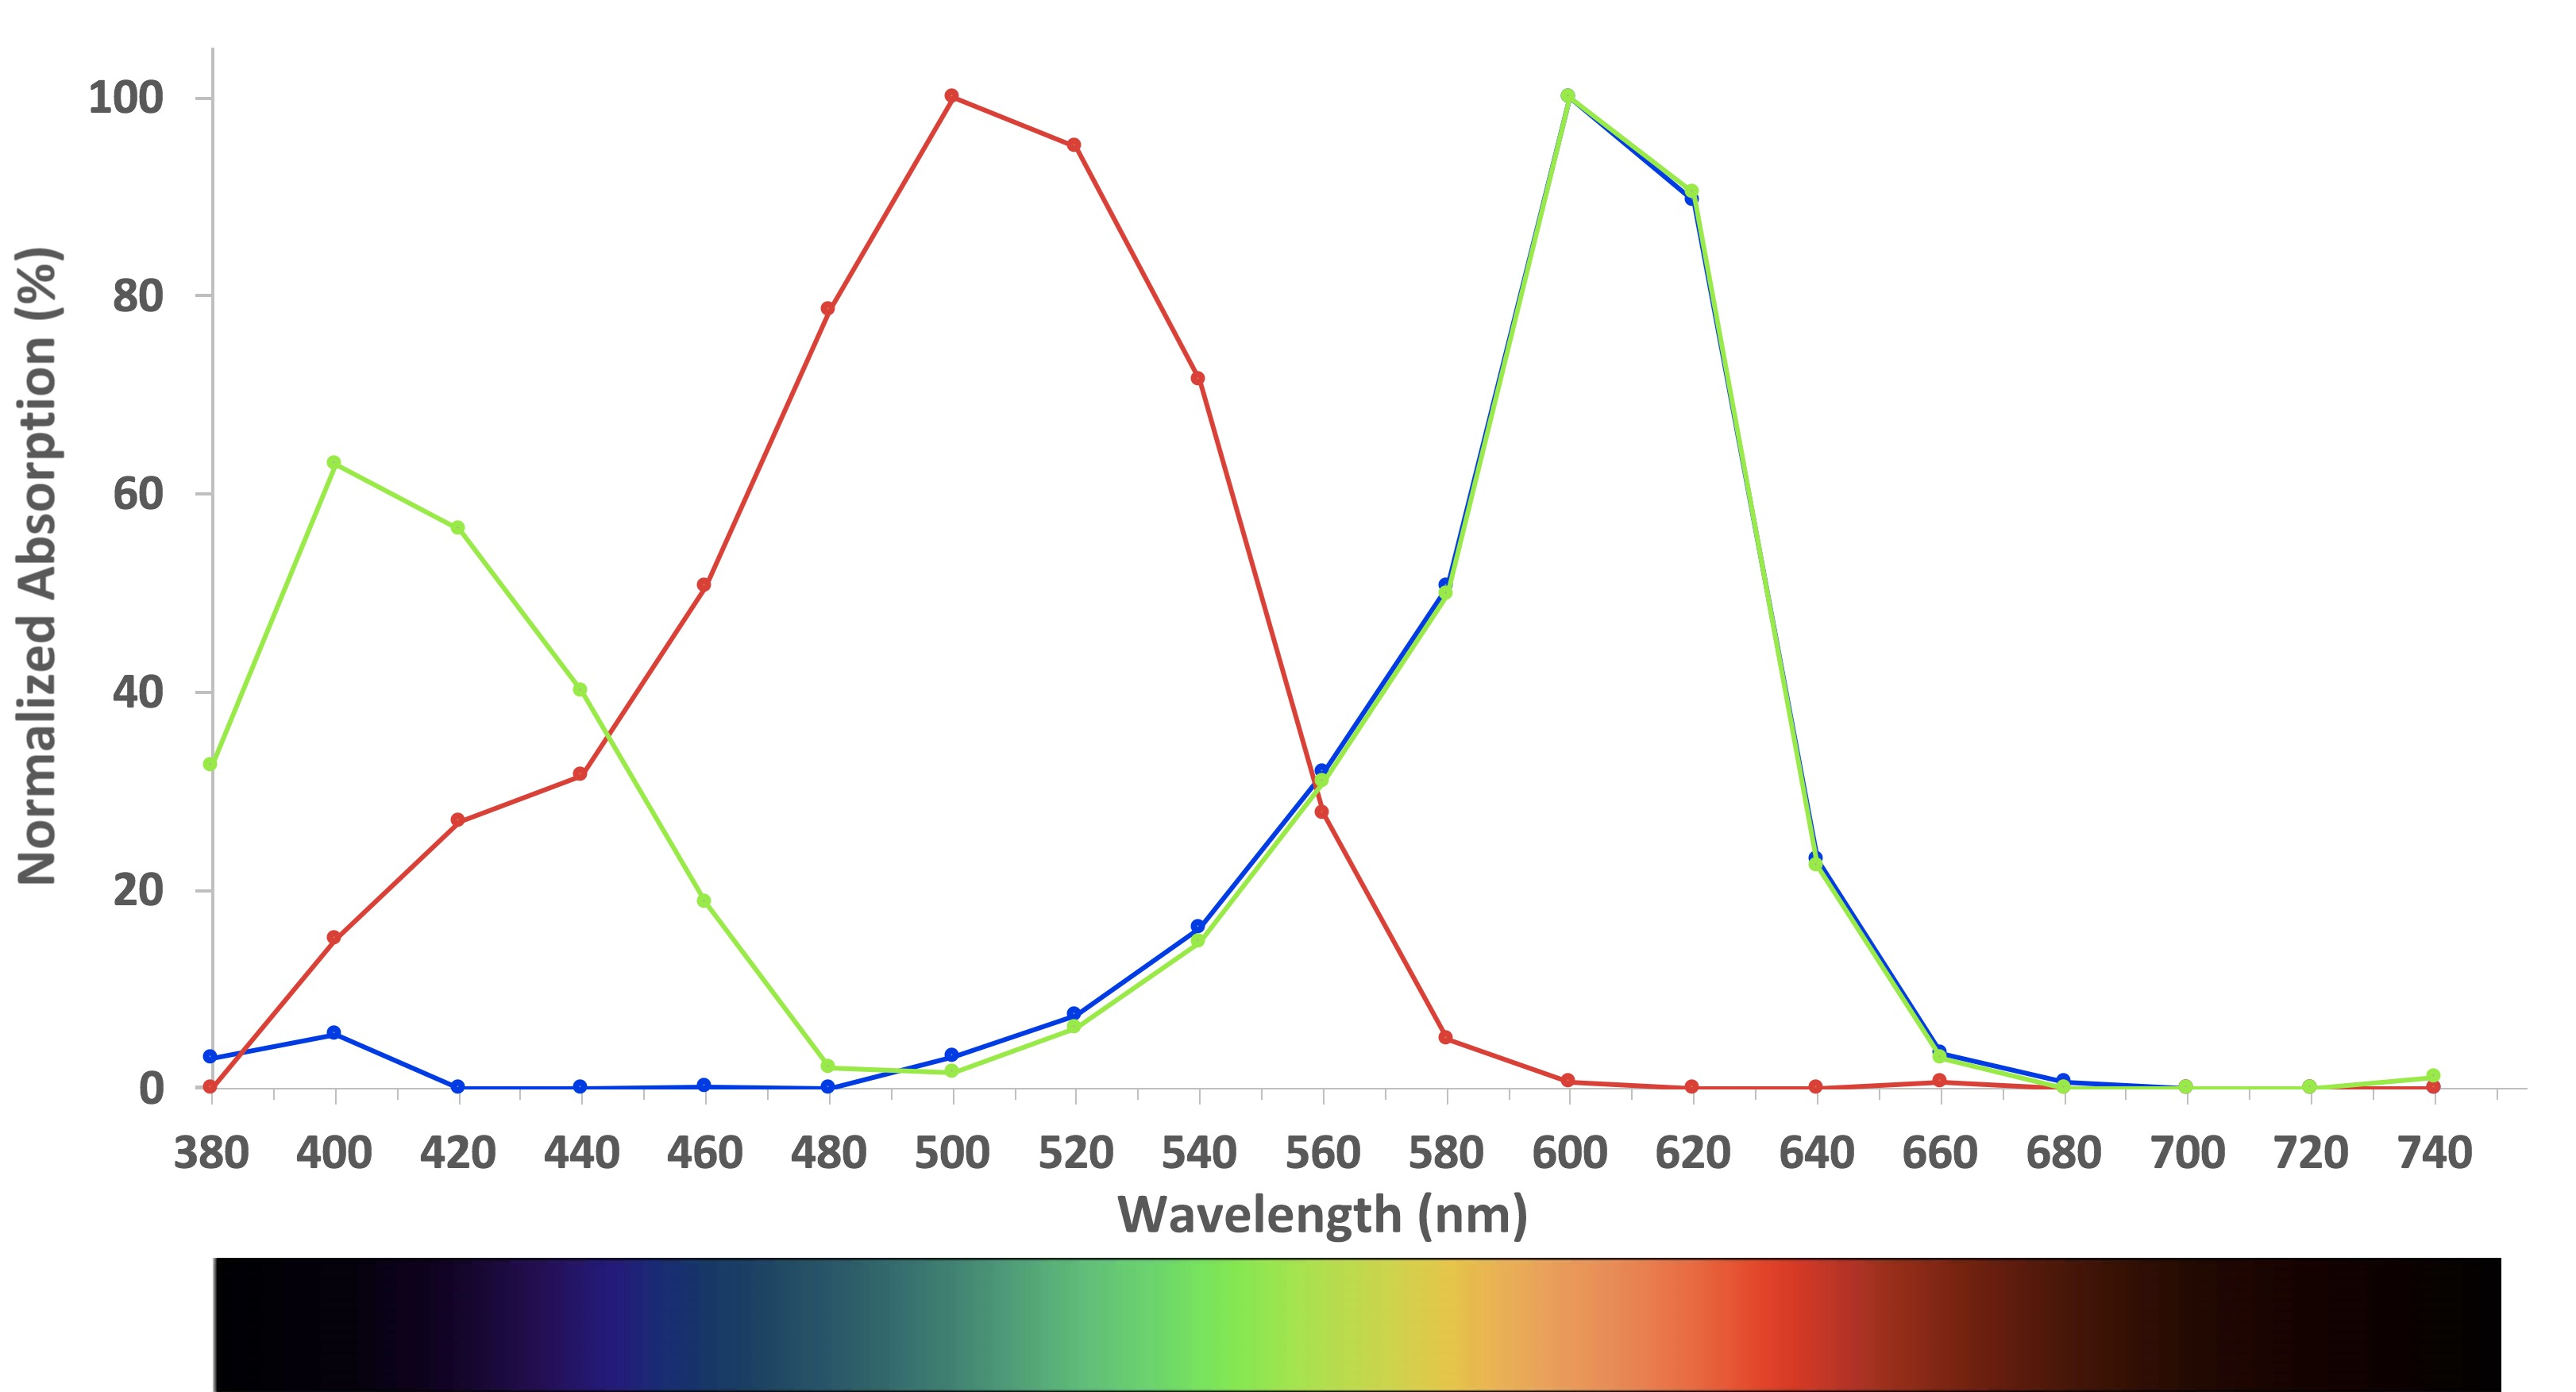
\includegraphics[width=0.7\linewidth]{./figures/photosynthesis/absorption_result} 

}

\caption{Normalized absorption of red, green and blue dye solutions. Compare these data with your own results.}\label{fig:apsorption}
\end{figure}

\section{Chromatography}\label{chromatography}

\href{https://en.wikipedia.org/wiki/Chromatography}{Chromatography} is a
laboratory technique for the separation of a mixture. The mixture is
dissolved in a fluid called the mobile phase, which carries it through a
structure holding another material called the stationary phase. The
various constituents of the mixture travel at different speeds, causing
them to separate. The separation is based on differential partitioning
between the mobile and stationary phases. Subtle differences in a
compound's partition coefficient result in differential retention on the
stationary phase and thus affect the separation. Chromatography may be
preparative or analytical. The purpose of preparative chromatography is
to separate the components of a mixture for later use and is thus a form
of purification. Analytical chromatography is done normally with smaller
amounts of material and is for establishing the presence or measuring
the relative proportions of analytes in a mixture.

In this experiment, we separate a mixture of food dyes (dark greenish
liquid. The mobile phase (separation buffer) is 1\% NaCl in water, the
stationary phase is chromatography paper.

\subsection{Experimental procedures}\label{experimental-procedures-27}

\begin{enumerate}
\def\labelenumi{\arabic{enumi}.}
\tightlist
\item
  Obtain a small beaker.
\item
  Add NaCl running buffer to the beaker until it reaches a height of
  about 5 mm.
\item
  Obtain a strip of chromatography paper and put it down on the bench.
\item
  Obtain the bottle containing the dark green food dye mixture.
\item
  Obtain a glass capillary and insert the tip of the capillary into the
  food dye mixture liquid. A little bit of dye will ascend into the
  capillary.
\item
  Remove the capillary and apply.
\item
  Touch the left side of the chromatography paper about 1 cm above its
  lower end with the tip of the capillary. A little bit of green liquid
  will spread out on the paper. Lift the capillary and touch the paper
  again just to the right of the dye you just applied. Repeat this until
  you have a horizontal line of dye from the left to the right side of
  the paper.
\item
  Place the chromatography paper into the beaker as shown below.
\item
  Observe how the running buffer moves up the paper and separates the
  dye mixture into three components (red, yellow and blue.
\end{enumerate}

\begin{figure}

{\centering 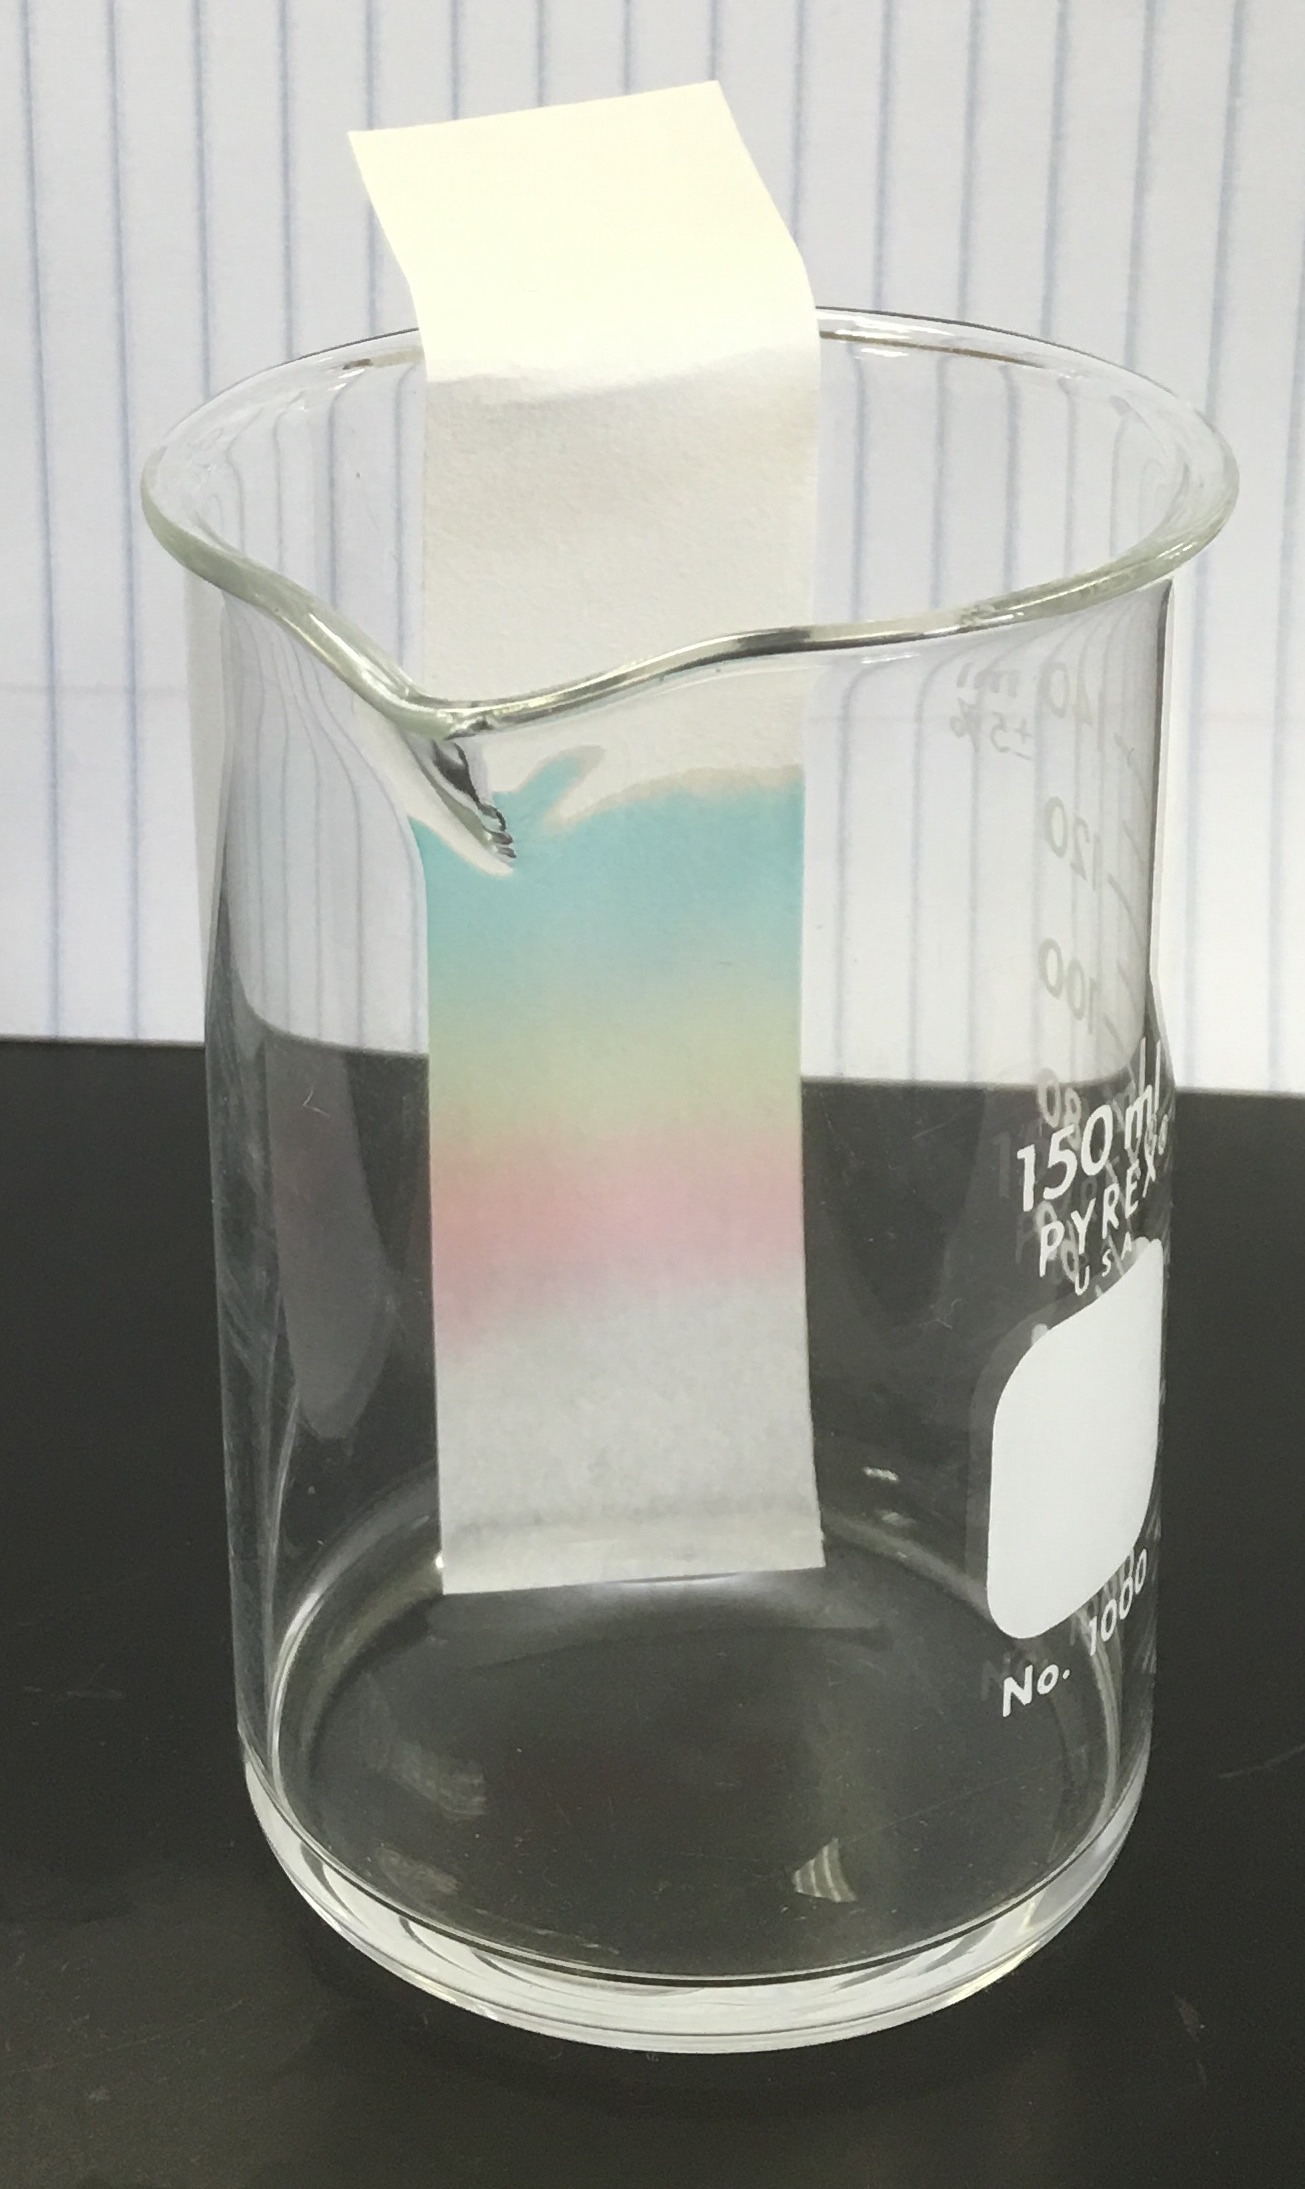
\includegraphics[width=0.7\linewidth]{./figures/photosynthesis/chromatography} 

}

\caption{Result of the Chromatography experiment.}\label{fig:chromatography}
\end{figure}

\section{Review Questions}\label{review-questions-5}

\begin{enumerate}
\def\labelenumi{\arabic{enumi}.}
\tightlist
\item
  What is light?
\item
  In your own words, describe the endproducts of photosynthesis.
\item
  In your own words, describe what happens in photosynthesis.
\item
  What is chlorophyll and what does it do?
\item
  Where inside of plant cells does photosynthesis happen?
\item
  What is chromatography and what is it used for?
\end{enumerate}

\chapter{Mitosis and Meiosis}\label{mitosis-and-meiosis}

\href{https://en.wikipedia.org/wiki/Mitosis}{Mitosis} is the part of the
cell cycle when replicated chromosomes are separated into two new
nuclei. In general, mitosis (division of the nucleus) is preceded by the
S stage of interphase (during which the DNA is replicated) and is often
accompanied or followed by cytokinesis, which divides the cytoplasm,
organelles and cell membrane into two new cells containing roughly equal
shares of these cellular components. Mitosis and cytokinesis together
define the mitotic (M) phase of an animal cell cycle (the division of
the mother cell into two daughter cells genetically identical to each
other). The process of mitosis is divided into stages corresponding to
the completion of one set of activities and the start of the next. These
stages are prophase, pro-metaphase, metaphase, anaphase, and telophase.

\href{https://en.wikipedia.org/wiki/Meiosis}{Meiosis} is a specialized
type of cell division that reduces the chromosome number by half,
creating four haploid cells, each genetically distinct from the parent
cell that gave rise to them. This process occurs in all sexually
reproducing single-celled and multicellular eukaryotes, including
animals, plants, and fungi. Errors in meiosis resulting in aneuploidy
are the leading known cause of miscarriage and the most frequent genetic
cause of developmental disabilities. In meiosis, DNA replication is
followed by two rounds of cell division to produce four daughter cells,
each with half the number of chromosomes as the original parent cell.
The two meiotic divisions are known as Meiosis I and Meiosis II. Before
meiosis begins, during S phase of the cell cycle, the DNA of each
chromosome is replicated so that it consists of two identical sister
chromatids, which remain held together through sister chromatid
cohesion. This S-phase can be referred to as ``premeiotic S-phase'' or
``meiotic S-phase''. Immediately following DNA replication, meiotic
cells enter a prolonged G2-like stage known as meiotic prophase. During
this time, homologous chromosomes pair with each other and undergo
genetic recombination, a programmed process in which DNA is cut and then
repaired, which allows them to exchange some of their genetic
information. A subset of recombination events results in crossovers,
which create physical links known as chiasmata (singular: chiasma, for
the Greek letter Chi (X)) between the homologous chromosomes. In most
organisms, these links are essential to direct each pair of homologous
chromosomes to segregate away from each other during Meiosis I,
resulting in two haploid cells that have half the number of chromosomes
as the parent cell. During Meiosis II, the cohesion between sister
chromatids is released and they segregate from one another, as during
mitosis. In some cases, all four of the meiotic products form gametes
such as sperm, spores, or pollen. In female animals, three of the four
meiotic products are typically eliminated by extrusion into polar
bodies, and only one cell develops to produce an ovum. Because the
number of chromosomes is halved during meiosis, gametes can fuse
(i.e.~fertilization) to form a diploid zygote that contains two copies
of each chromosome, one from each parent. Thus, alternating cycles of
meiosis and fertilization enable sexual reproduction, with successive
generations maintaining the same number of chromosomes. For example,
diploid human cells contain 23 pairs of chromosomes including 1 pair of
sex chromosomes (46 total), half of maternal origin and half of paternal
origin. Meiosis produces haploid gametes (ova or sperm) that contain one
set of 23 chromosomes. When two gametes (an egg and a sperm) fuse, the
resulting zygote is once again diploid, with the mother and father each
contributing 23 chromosomes. This same pattern, but not the same number
of chromosomes, occurs in all organisms that utilize meiosis.

\section{View Prepared Slides}\label{view-prepared-slides-1}

\begin{enumerate}
\def\labelenumi{\arabic{enumi}.}
\tightlist
\item
  View the onion root tip and observe the different stages of mitosis
  (Figure \ref{fig:tip}).
\end{enumerate}

\begin{figure}

{\centering 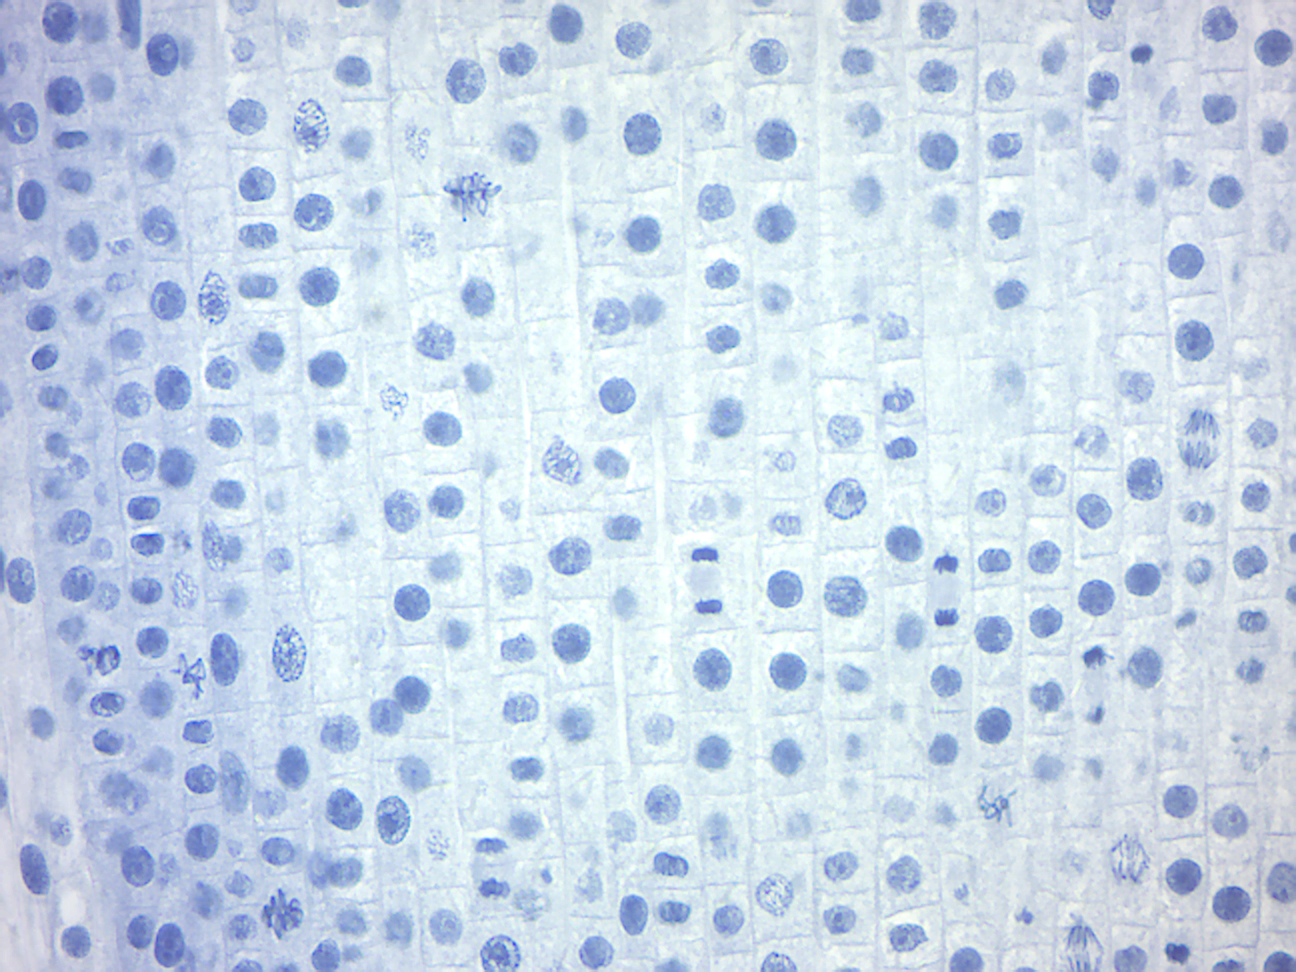
\includegraphics[width=0.7\linewidth]{./figures/mitosis/Onion_root_tip} 

}

\caption{Onion root tip}\label{fig:tip}
\end{figure}

\begin{enumerate}
\def\labelenumi{\arabic{enumi}.}
\setcounter{enumi}{1}
\tightlist
\item
  View the fish blastodisc and observe the different stages of mitosis
  (Figure \ref{fig:blastodisc}).
\end{enumerate}

\begin{figure}

{\centering 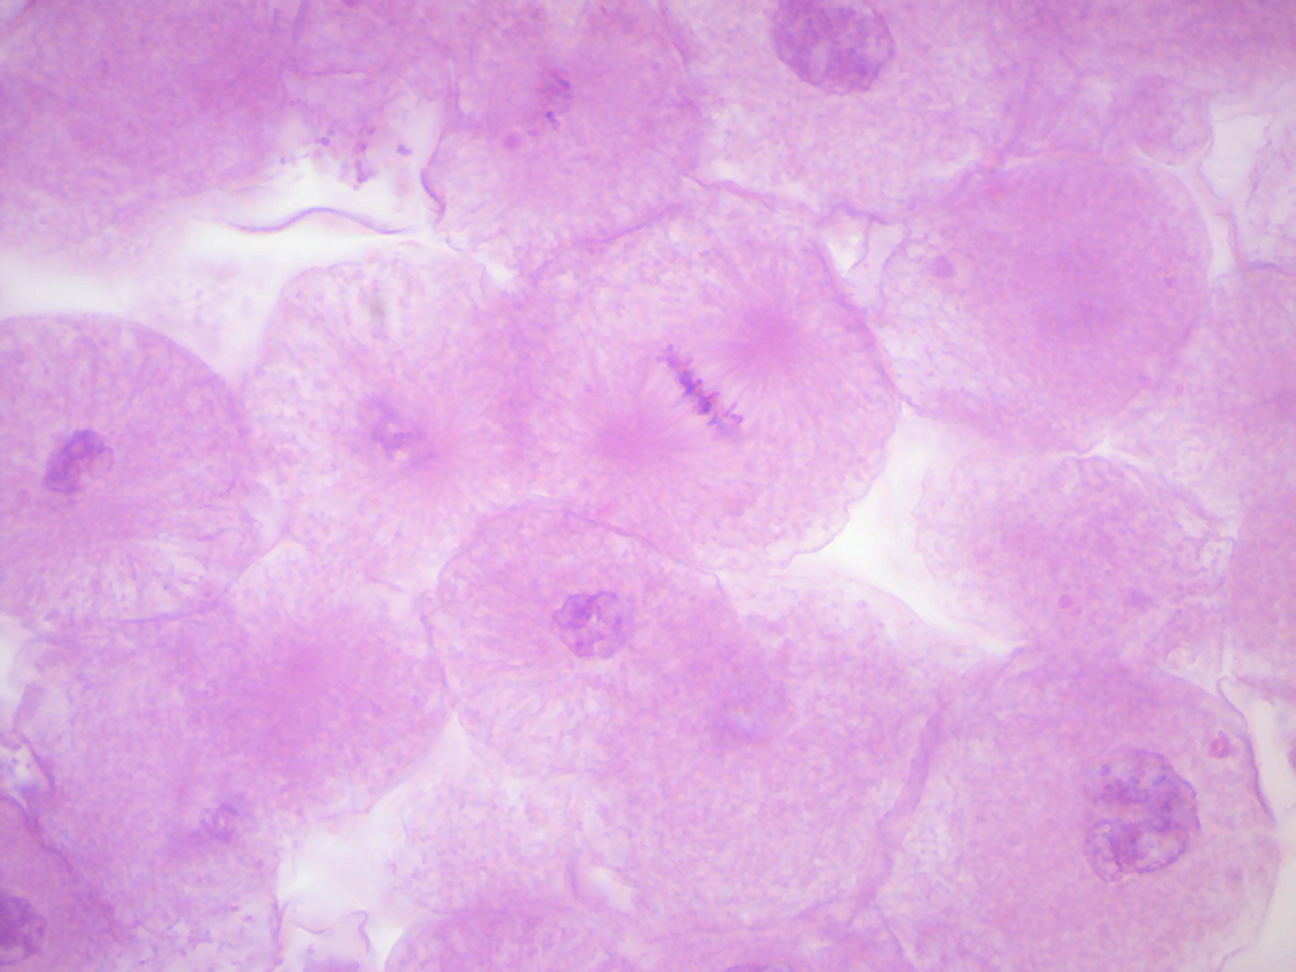
\includegraphics[width=0.7\linewidth]{./figures/mitosis/Fish_blastodisc} 

}

\caption{Fish blastodisc}\label{fig:blastodisc}
\end{figure}

\section{Preparing an Onion root tip
squash}\label{preparing-an-onion-root-tip-squash}

\subsection{Experimental procedures}\label{experimental-procedures-28}

\begin{enumerate}
\def\labelenumi{\arabic{enumi}.}
\tightlist
\item
  Obtain an onion bulb that shows some roots.
\item
  Cut off a root tip and place it on a clean slide.
\item
  Cut off 1mm to 2mm of the root tip and throw away the upper portion of
  the root.
\item
  Cover the root tip with four drops of 1 N HCl and warm the slide over
  an alcohol burner flame for 1 minute. Do not boil.
\item
  Blot off the excess HCl and cover the root tip with 0.5\% aqueous
  toluidine blue.
\item
  Again, pass the slide through the alcohol burner flame for 1 minute
  without boiling.
\item
  Blot off the excess stain, add a drop of fresh stain, and apply a
  coverslip.
\item
  Cover the slide with a paper towel and carefully squash the coverslip
  firmly with your thumb.
\item
  Examine the slide for the stages of mitosis as well as interphase and
  cytokinesis.
\end{enumerate}

\begin{figure}

{\centering 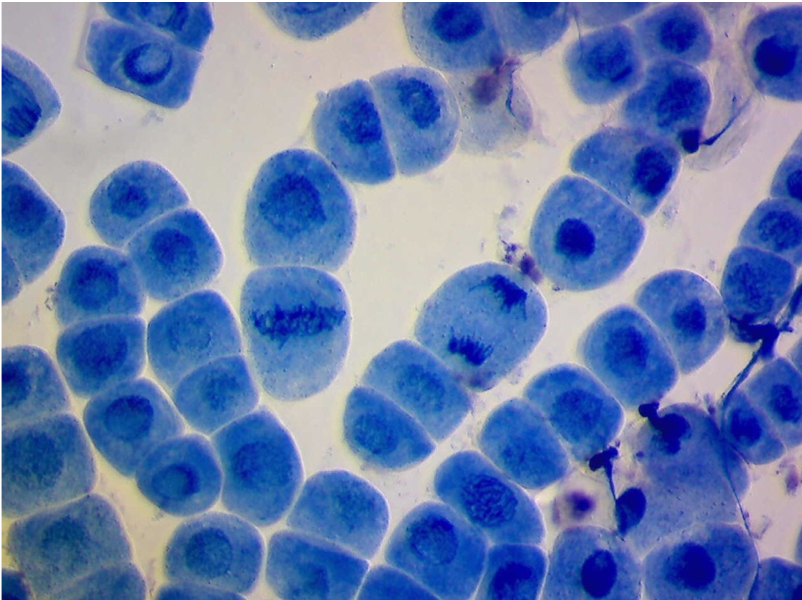
\includegraphics[width=0.7\linewidth]{./figures/mitosis/Onion_root_tip_spread} 

}

\caption{Several different phases of mitosis are visible in this onion root tip spread.}\label{fig:spread}
\end{figure}

\section{Review Questions}\label{review-questions-6}

\begin{enumerate}
\def\labelenumi{\arabic{enumi}.}
\tightlist
\item
  What is mitosis and what is its outcome?
\item
  What is meiosis and what is its outcome?
\item
  What is homologous recombination and what is its outcome?
\item
  What do the terms haploid and diploid mean?
\item
  Are you a haploid or a diploid organism?
\item
  What are gametes?
\item
  What is a zygote?
\end{enumerate}

\chapter{Mendelian Genetics}\label{mendelian-genetics}

In this experiment, we will use maize \emph{Zea mays} subsp. mays, from
Spanish: maíz after Taíno mahiz), also known as corn to study
\href{https://en.wikipedia.org/wiki/Mendelian_inheritance}{Mendelian
inheritance}. This cereal grain was first domesticated by indigenous
peoples in southern Mexico about 10,000 years ago. The leafy stalk of
the plant produces separate pollen and ovuliferous inflorescences or
ears, which are fruits, yielding kernels or seeds. Maize has become a
staple food in many parts of the world, with total production surpassing
that of wheat or rice. However, not all of this maize is consumed
directly by humans. Some of the maize production is used for corn
ethanol, animal feed and other maize products, such as corn starch and
corn syrup. The six major types of corn are dent corn, flint corn, pod
corn, popcorn, flour corn, and sweet corn.

The principles of Mendelian inheritance were named for and first derived
by \href{https://en.wikipedia.org/wiki/Gregor_Mendel}{Gregor Johann
Mendel}, a nineteenth-century Moravian monk who formulated his ideas
after conducting simple hybridisation experiments with pea plants
(\emph{Pisum sativum}) he had planted in the garden of his monastery.
Between 1856 and 1863, Mendel cultivated and tested some 5,000 pea
plants. From these experiments, he induced two generalizations which
later became known as Mendel's Principles of Heredity or Mendelian
inheritance (Table \ref{tab:mendel}). He described these principles in a
two-part paper, Versuche über Pflanzen-Hybriden (Experiments on Plant
Hybridization), that he read to the Natural History Society of Brno on 8
February and 8 March 1865, and which was published in 1866. Mendel's
conclusions were largely ignored by the vast majority of scientists at
the time. In 1900, however, his work was ``re-discovered'' by three
European scientists, Hugo de Vries, Carl Correns, and Erich von
Tschermak.

Mendel discovered that, when he crossed purebred white flower and purple
flower pea plants (the parental or P generation), the result was not a
blend. Rather than being a mix of the two, the offspring (known as the
F1 generation) was purple-flowered. When Mendel self-fertilized the F1
generation pea plants, he obtained a purple flower to white flower ratio
in the F2 generation of 3 to 1. In the first experiment, we will examine
the F2 generation resulting from the F1 generation obtained from a
parental generation of yellow and purple corn.

He then conceived the idea of heredity units, which he called
``factors''. Mendel found that there are alternative forms of
factors---now called genes---that account for variations in inherited
characteristics. For example, the gene for flower color in pea plants
exists in two forms, one for purple and the other for white. The
alternative ``forms'' are now called alleles. For each biological trait,
an organism inherits two alleles, one from each parent. These alleles
may be the same or different. An organism that has two identical alleles
for a gene is said to be homozygous for that gene (and is called a
homozygote). An organism that has two different alleles for a gene is
said be heterozygous for that gene (and is called a heterozygote).

Mendel hypothesized that allele pairs separate randomly, or segregate,
from each other during the production of gametes: egg and sperm. Because
allele pairs separate during gamete production, a sperm or egg carries
only one allele for each inherited trait. When sperm and egg unite at
fertilization, each contributes its allele, restoring the paired
condition in the offspring. This is called the Law of Segregation.
Mendel also found that each pair of alleles segregates independently of
the other pairs of alleles during gamete formation. This is known as the
Law of Independent Assortment. In the second experiment, we will observe
this law exemplified by a dihybrid cross of corn.

The genotype of an individual is made up of the many alleles it
possesses. An individual's physical appearance, or phenotype, is
determined by its alleles as well as by its environment. The presence of
an allele does not mean that the trait will be expressed in the
individual that possesses it. If the two alleles of an inherited pair
differ (the heterozygous condition), then one determines the organism's
appearance and is called the dominant allele; the other has no
noticeable effect on the organism's appearance and is called the
recessive allele. Thus, in the example above the dominant purple flower
allele will hide the phenotypic effects of the recessive white flower
allele. This is known as the Law of Dominance but it is not a
transmission law: it concerns the expression of the genotype. The upper
case letters are used to represent dominant alleles whereas the
lowercase letters are used to represent recessive alleles.

\begin{longtable}[]{@{}ll@{}}
\caption{\label{tab:mendel} Mendel's laws of inheritance.}\tabularnewline
\toprule
\begin{minipage}[b]{0.05\columnwidth}\raggedright\strut
Law\strut
\end{minipage} & \begin{minipage}[b]{0.14\columnwidth}\raggedright\strut
Definition\strut
\end{minipage}\tabularnewline
\midrule
\endfirsthead
\toprule
\begin{minipage}[b]{0.05\columnwidth}\raggedright\strut
Law\strut
\end{minipage} & \begin{minipage}[b]{0.14\columnwidth}\raggedright\strut
Definition\strut
\end{minipage}\tabularnewline
\midrule
\endhead
\begin{minipage}[t]{0.05\columnwidth}\raggedright\strut
Law of segregation\strut
\end{minipage} & \begin{minipage}[t]{0.14\columnwidth}\raggedright\strut
During gamete formation, the alleles for each gene segregate from each
other so that each gamete carries only one allele for each gene.\strut
\end{minipage}\tabularnewline
\begin{minipage}[t]{0.05\columnwidth}\raggedright\strut
Law of independent assortment\strut
\end{minipage} & \begin{minipage}[t]{0.14\columnwidth}\raggedright\strut
Genes for different traits can segregate independently during the
formation of gametes.\strut
\end{minipage}\tabularnewline
\begin{minipage}[t]{0.05\columnwidth}\raggedright\strut
Law of dominance\strut
\end{minipage} & \begin{minipage}[t]{0.14\columnwidth}\raggedright\strut
Some alleles are dominant while others are recessive; an organism with
at least one dominant allele will display the effect of the dominant
allele.\strut
\end{minipage}\tabularnewline
\bottomrule
\end{longtable}

\section{Punnett square}\label{punnett-square}

The \href{https://en.wikipedia.org/wiki/Punnett_square}{Punnett square}
(Figures \ref{fig:punnett} and \ref{fig:punnettF1}) is a visual
representation of Mendelian inheritance and used to predict an outcome
of a particular cross or breeding experiment. It is named after
\href{https://en.wikipedia.org/wiki/Reginald_Punnett}{Reginald C.
Punnett}, who devised the approach. In our first experiment, both
parents are homozygous, one carrying two copies of the dominant allele
(R), the other two copies of the recessive (r) allele. Each parent can
only make gametes that have either the R (purple) or r (yellow) allele.
The Punnett square for the parental cross is shown in Figure
\ref{fig:punnett}

\begin{figure}

{\centering 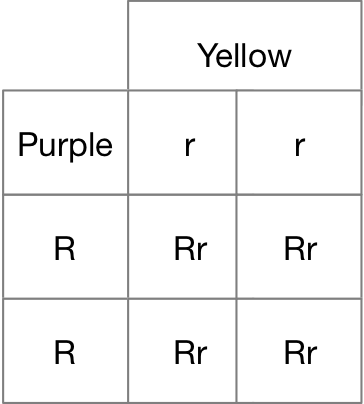
\includegraphics[width=0.7\linewidth]{./figures/mendel/Punnett} 

}

\caption{Punnett square for homozygous cross.}\label{fig:punnett}
\end{figure}

The squares containing the single letters represent the possible
gametes. The squares with two letters represent the zygotes resulting
from the combination of the respective gametes. It can be easily seen
that all offspring will be heterozygous (Rr) and therefore purple. The
Punnett square for the F1 cross is depicted in Figure
\ref{fig:punnettF1}

\begin{figure}

{\centering 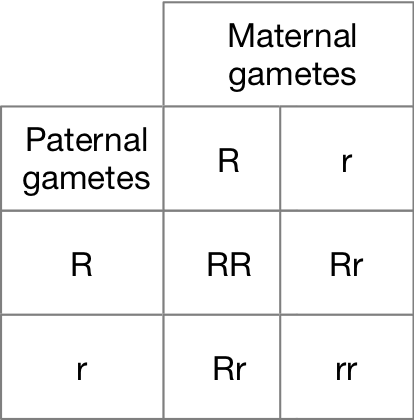
\includegraphics[width=0.7\linewidth]{./figures/mendel/PunnettF1} 

}

\caption{Punnett square for heterozygous cross.}\label{fig:punnettF1}
\end{figure}

\section{Monohybrid cross (Experiment
1)}\label{monohybrid-cross-experiment-1}

A \href{https://en.wikipedia.org/wiki/Monohybrid_cross}{monohybrid
cross} is a mating between two individuals with different variations at
one genetic trait of interest. The character(s) being studied in a
monohybrid cross are governed by two or multiple variations for a single
locus. A cross between two parents possessing a pair of contrasting
characters is known as monohybrid cross. To carry out such a cross, each
parent is chosen to be homozygous or true breeding for a given trait
(locus). When a cross satisfies the conditions for a monohybrid cross,
it is usually detected by a characteristic distribution of
second-generation (F2) offspring that is sometimes called the monohybrid
ratio.

Generally, the monohybrid cross is used to determine the dominance
relationship between two alleles. The cross begins with the parental (P)
generation. One parent is homozygous for one allele, and the other
parent is homozygous for the other allele. The offspring make up the
first filial (F1) generation. Every member of the F1 generation is
heterozygous and the phenotype of the F1 generation expresses the
dominant trait. Crossing two members of the F1 generation produces the
second filial (F2) generation. Probability theory predicts that three
quarters of the F2 generation will have the dominant allele's phenotype.
And the remaining quarter of the F2s will have the recessive allele's
phenotype. This predicted 3:1 phenotypic ratio assumes Mendelian
inheritance.

In the first experiment, we will study the result obtained from a
monohybrid cross. A strain of corn producing pure purple kernels (RR) is
crossed with a strain producing pure yellow kernels (rr). Purple is
dominant with the resulting F1 ears all bearing purple kernels. These
plants that are heterozygous for a single trait are called monohybrids.
When the F1 is self-pollinated, the resulting F2 ears bear both purple
and yellow kernels (Figure \ref{fig:monohybrid}).

\begin{figure}

{\centering 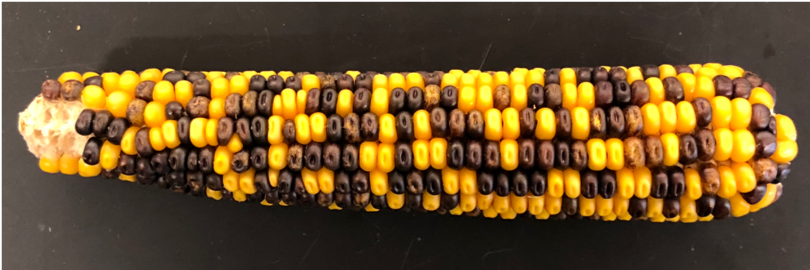
\includegraphics[width=0.7\linewidth]{./figures/mendel/Monohybrid_cross} 

}

\caption{Monohybrid cross}\label{fig:monohybrid}
\end{figure}

\subsection{Experimental procedures}\label{experimental-procedures-29}

\begin{enumerate}
\def\labelenumi{\arabic{enumi}.}
\tightlist
\item
  Count the number of purple and yellow kernels on one row of the F2 ear
  without removing the kernels.
\item
  Determine the ratio of purple to yellow.
\item
  Now tabulate the numbers obtained by each of your class mates in Table
  \ref{tab:mono} and add these figures to get a total.
\item
  Using the total numbers, determine a ratio of purple to yellow.
\end{enumerate}

\begin{longtable}[]{@{}cccc@{}}
\caption{\label{tab:mono} Monohybrid cross.}\tabularnewline
\toprule
Row \# & purple & yellow & ratio\tabularnewline
\midrule
\endfirsthead
\toprule
Row \# & purple & yellow & ratio\tabularnewline
\midrule
\endhead
1 & & &\tabularnewline
2 & & &\tabularnewline
3 & & &\tabularnewline
\ldots{} & & &\tabularnewline
7 & & &\tabularnewline
8 & & &\tabularnewline
9 & & &\tabularnewline
Total & & &\tabularnewline
\bottomrule
\end{longtable}

\section{Dihybrid cross (Experiment
2)}\label{dihybrid-cross-experiment-2}

In the second experiment, we will study the result obtained from a
\href{https://en.wikipedia.org/wiki/Dihybrid_cross}{dihybrid cross}. A
dihybrid cross is a cross between two different lines (varieties,
strains) that differ in two observed traits. In the name ``Dihybrid
cross'', the ``di'' indicates that there are two traits involved (in our
example designated R and Su), the ``hybrid'' means that each trait has
two different alleles (in our example R and r, or Su and su), and
``cross'' means that there are two individuals who are combining or
``crossing'' their genetic information. In our example, a pure strain of
corn producing purple-starchy kernels (RR SuSu) is crossed with a pure
strain producing yellow-sweet (rr susu). The starchy seeds are smooth,
the sweet seeds are wrinkled. The resulting F1 ears all bear
purple-starchy (smooth) kernels. Plants that are heterozygous for two
traits are called dihybrids. When the F1 is self-pollinated, the
resulting F2 generation contains various combinations (Figure
\ref{fig:dihybrid}).

\begin{figure}

{\centering 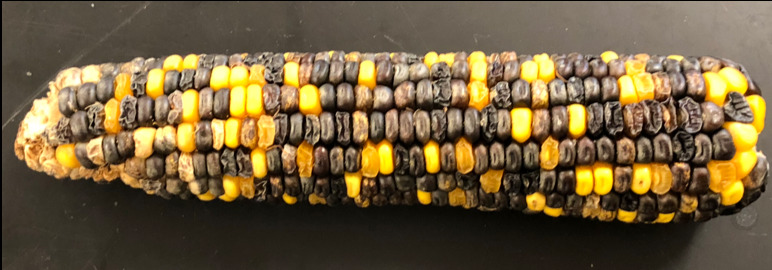
\includegraphics[width=0.7\linewidth]{./figures/mendel/Dihybrid_cross} 

}

\caption{Dihybrid cross}\label{fig:dihybrid}
\end{figure}

The rules of meiosis, as they apply to the dihybrid, are codified in
Mendel's first law and Mendel's second law, which are also called the
Law of Segregation and the Law of Independent Assortment, respectively
(Table \ref{tab:mendel}). For genes on separate chromosomes, each allele
pair showed independent segregation. If the first filial generation (F1
generation) produces four identical offspring, the second filial
generation, which occurs by crossing the members of the first filial
generation, shows a phenotypic (appearance) ratio of \textbf{9:3:3:1},
where:

\begin{itemize}
\tightlist
\item
  the \textbf{9} represents the proportion of individuals displaying
  both dominant traits
\item
  the first \textbf{3} represents the individuals displaying the first
  dominant trait and the second recessive trait
\item
  the second \textbf{3} represents those displaying the first recessive
  trait and second dominant trait
\item
  the \textbf{1} represents the homozygous, displaying both recessive
  traits.
\end{itemize}

\subsection{Experimental procedures}\label{experimental-procedures-30}

\begin{enumerate}
\def\labelenumi{\arabic{enumi}.}
\tightlist
\item
  Carefully count the number of kernels of each phenotype appearing on a
  row of F2 ear. Tabulate the results and determine the totals and total
  ratios in Table \ref{tab:di}.
\end{enumerate}

\begin{longtable}[]{@{}clllll@{}}
\caption{\label{tab:di} Dihybrid cross.}\tabularnewline
\toprule
\begin{minipage}[b]{0.05\columnwidth}\centering\strut
Row \#\strut
\end{minipage} & \begin{minipage}[b]{0.19\columnwidth}\raggedright\strut
purple and starchy (smooth)\strut
\end{minipage} & \begin{minipage}[b]{0.19\columnwidth}\raggedright\strut
purple and sweet (wrinkled)\strut
\end{minipage} & \begin{minipage}[b]{0.19\columnwidth}\raggedright\strut
yellow and starchy (smooth)\strut
\end{minipage} & \begin{minipage}[b]{0.19\columnwidth}\raggedright\strut
yellow and sweet (wrinkled)\strut
\end{minipage} & \begin{minipage}[b]{0.04\columnwidth}\raggedright\strut
ratio\strut
\end{minipage}\tabularnewline
\midrule
\endfirsthead
\toprule
\begin{minipage}[b]{0.05\columnwidth}\centering\strut
Row \#\strut
\end{minipage} & \begin{minipage}[b]{0.19\columnwidth}\raggedright\strut
purple and starchy (smooth)\strut
\end{minipage} & \begin{minipage}[b]{0.19\columnwidth}\raggedright\strut
purple and sweet (wrinkled)\strut
\end{minipage} & \begin{minipage}[b]{0.19\columnwidth}\raggedright\strut
yellow and starchy (smooth)\strut
\end{minipage} & \begin{minipage}[b]{0.19\columnwidth}\raggedright\strut
yellow and sweet (wrinkled)\strut
\end{minipage} & \begin{minipage}[b]{0.04\columnwidth}\raggedright\strut
ratio\strut
\end{minipage}\tabularnewline
\midrule
\endhead
\begin{minipage}[t]{0.05\columnwidth}\centering\strut
1\strut
\end{minipage} & \begin{minipage}[t]{0.19\columnwidth}\raggedright\strut
\strut
\end{minipage} & \begin{minipage}[t]{0.19\columnwidth}\raggedright\strut
\strut
\end{minipage} & \begin{minipage}[t]{0.19\columnwidth}\raggedright\strut
\strut
\end{minipage} & \begin{minipage}[t]{0.19\columnwidth}\raggedright\strut
\strut
\end{minipage} & \begin{minipage}[t]{0.04\columnwidth}\raggedright\strut
\strut
\end{minipage}\tabularnewline
\begin{minipage}[t]{0.05\columnwidth}\centering\strut
2\strut
\end{minipage} & \begin{minipage}[t]{0.19\columnwidth}\raggedright\strut
\strut
\end{minipage} & \begin{minipage}[t]{0.19\columnwidth}\raggedright\strut
\strut
\end{minipage} & \begin{minipage}[t]{0.19\columnwidth}\raggedright\strut
\strut
\end{minipage} & \begin{minipage}[t]{0.19\columnwidth}\raggedright\strut
\strut
\end{minipage} & \begin{minipage}[t]{0.04\columnwidth}\raggedright\strut
\strut
\end{minipage}\tabularnewline
\begin{minipage}[t]{0.05\columnwidth}\centering\strut
3\strut
\end{minipage} & \begin{minipage}[t]{0.19\columnwidth}\raggedright\strut
\strut
\end{minipage} & \begin{minipage}[t]{0.19\columnwidth}\raggedright\strut
\strut
\end{minipage} & \begin{minipage}[t]{0.19\columnwidth}\raggedright\strut
\strut
\end{minipage} & \begin{minipage}[t]{0.19\columnwidth}\raggedright\strut
\strut
\end{minipage} & \begin{minipage}[t]{0.04\columnwidth}\raggedright\strut
\strut
\end{minipage}\tabularnewline
\begin{minipage}[t]{0.05\columnwidth}\centering\strut
\ldots{}\strut
\end{minipage} & \begin{minipage}[t]{0.19\columnwidth}\raggedright\strut
\strut
\end{minipage} & \begin{minipage}[t]{0.19\columnwidth}\raggedright\strut
\strut
\end{minipage} & \begin{minipage}[t]{0.19\columnwidth}\raggedright\strut
\strut
\end{minipage} & \begin{minipage}[t]{0.19\columnwidth}\raggedright\strut
\strut
\end{minipage} & \begin{minipage}[t]{0.04\columnwidth}\raggedright\strut
\strut
\end{minipage}\tabularnewline
\begin{minipage}[t]{0.05\columnwidth}\centering\strut
7\strut
\end{minipage} & \begin{minipage}[t]{0.19\columnwidth}\raggedright\strut
\strut
\end{minipage} & \begin{minipage}[t]{0.19\columnwidth}\raggedright\strut
\strut
\end{minipage} & \begin{minipage}[t]{0.19\columnwidth}\raggedright\strut
\strut
\end{minipage} & \begin{minipage}[t]{0.19\columnwidth}\raggedright\strut
\strut
\end{minipage} & \begin{minipage}[t]{0.04\columnwidth}\raggedright\strut
\strut
\end{minipage}\tabularnewline
\begin{minipage}[t]{0.05\columnwidth}\centering\strut
8\strut
\end{minipage} & \begin{minipage}[t]{0.19\columnwidth}\raggedright\strut
\strut
\end{minipage} & \begin{minipage}[t]{0.19\columnwidth}\raggedright\strut
\strut
\end{minipage} & \begin{minipage}[t]{0.19\columnwidth}\raggedright\strut
\strut
\end{minipage} & \begin{minipage}[t]{0.19\columnwidth}\raggedright\strut
\strut
\end{minipage} & \begin{minipage}[t]{0.04\columnwidth}\raggedright\strut
\strut
\end{minipage}\tabularnewline
\begin{minipage}[t]{0.05\columnwidth}\centering\strut
9\strut
\end{minipage} & \begin{minipage}[t]{0.19\columnwidth}\raggedright\strut
\strut
\end{minipage} & \begin{minipage}[t]{0.19\columnwidth}\raggedright\strut
\strut
\end{minipage} & \begin{minipage}[t]{0.19\columnwidth}\raggedright\strut
\strut
\end{minipage} & \begin{minipage}[t]{0.19\columnwidth}\raggedright\strut
\strut
\end{minipage} & \begin{minipage}[t]{0.04\columnwidth}\raggedright\strut
\strut
\end{minipage}\tabularnewline
\begin{minipage}[t]{0.05\columnwidth}\centering\strut
Total\strut
\end{minipage} & \begin{minipage}[t]{0.19\columnwidth}\raggedright\strut
\strut
\end{minipage} & \begin{minipage}[t]{0.19\columnwidth}\raggedright\strut
\strut
\end{minipage} & \begin{minipage}[t]{0.19\columnwidth}\raggedright\strut
\strut
\end{minipage} & \begin{minipage}[t]{0.19\columnwidth}\raggedright\strut
\strut
\end{minipage} & \begin{minipage}[t]{0.04\columnwidth}\raggedright\strut
\strut
\end{minipage}\tabularnewline
\bottomrule
\end{longtable}

\section{Blood Typing (Experiment 3)}\label{blood-typing-experiment-3}

In this experiment, we will determine the ABO properties of four
(artificial) blood samples.




\begin{figure}

{\centering 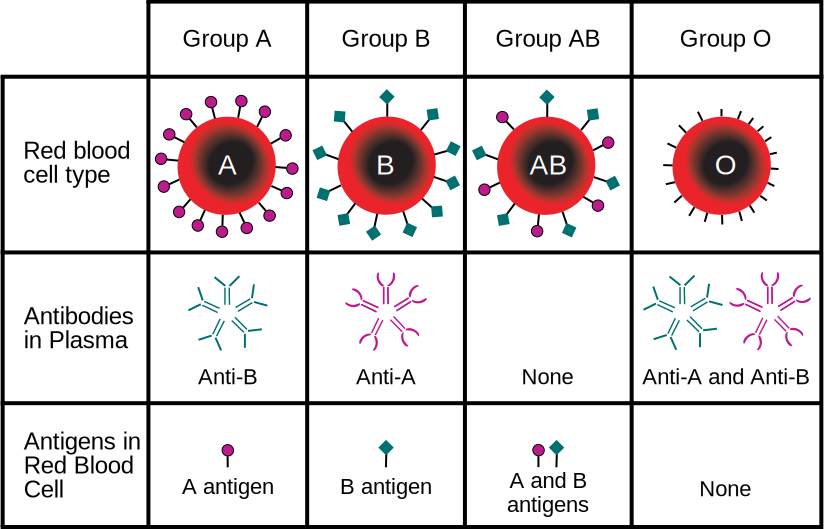
\includegraphics[width=0.7\linewidth]{./figures/mendel/blood_type} 

}

\caption{Blood type (or blood group) is determined, in part, by the
ABO blood group antigens present on red blood cells.}\label{fig:type}
\end{figure}

A \href{https://en.wikipedia.org/wiki/Blood_type}{blood type} (also
called a blood group)
(\href{https://commons.wikimedia.org/wiki/File:ABO_blood_type.svg}{Figure
\ref{fig:type}}) is a classification of blood based on the presence and
absence of antibodies and also based on the presence or absence of
inherited antigenic substances on the surface of red blood cells (RBCs).
These antigens may be proteins, carbohydrates, glycoproteins, or
glycolipids, depending on the blood group system. Some of these antigens
are also present on the surface of other types of cells of various
tissues. Blood types are inherited and represent contributions from both
parents. A total of 35 human blood group systems are now recognized by
the International Society of Blood Transfusion (ISBT). The two most
important ones are ABO and the RhD (``Rhesus'') antigen; they determine
someone's blood type (A, B, AB and O, with +, - or Null denoting RhD
status).

\subsection{Experimental procedures}\label{experimental-procedures-31}

\begin{enumerate}
\def\labelenumi{\arabic{enumi}.}
\tightlist
\item
  Using the dropper vial, place a drop of the first synthetic blood
  sample in each well of the blood-typing slide (Figure
  \ref{fig:typing}). Replace the cap on the dropper vial. Always replace
  the cap on one vial before opening the next vial, to prevent
  cross-contamination.
\item
  Add a drop of synthetic anti-A (blue) to the well labeled A. Replace
  the cap.
\item
  Add a drop of synthetic anti-B serum (yellow) to the well labeled B.
  Replace the cap.
\item
  Add a drop of synthetic anti-D (Rh) serum (clear) to the well labeled
  Rh. Replace the cap.
\item
  Using a mixing stick of a different color for each well (blue for
  anti-A, yellow for anti-B, white for anti-Rh), gently stir the
  synthetic blood and anti-serum drops for 30 seconds. Remember to
  discard each mixing stick after a single use to avoid contamination of
  your samples.
\item
  Carefully examine the thin films of liquid mixture left behind:

  \begin{itemize}
  \tightlist
  \item
    If a film remains uniform in appearance, there is no agglutination.
  \item
    If the sample appears granular, agglutination has occurred.
  \end{itemize}
\item
  Answer yes or no as to whether agglutination occurred in each sample.
  A positive agglutination reaction indicates the blood type.
\item
  Record the results for the first blood sample in Table
  \ref{tab:blood}.
\item
  Determine the blood type of the sample using the results that you
  entered in Table \ref{tab:blood}.
\item
  Thoroughly rinse the blood-typing slide and repeat steps 1 through 7
  for synthetic blood samples 2, 3, and 4, recording the results of each
  test as you go (and rinsing the slide after each sample).
\end{enumerate}

\begin{figure}

{\centering 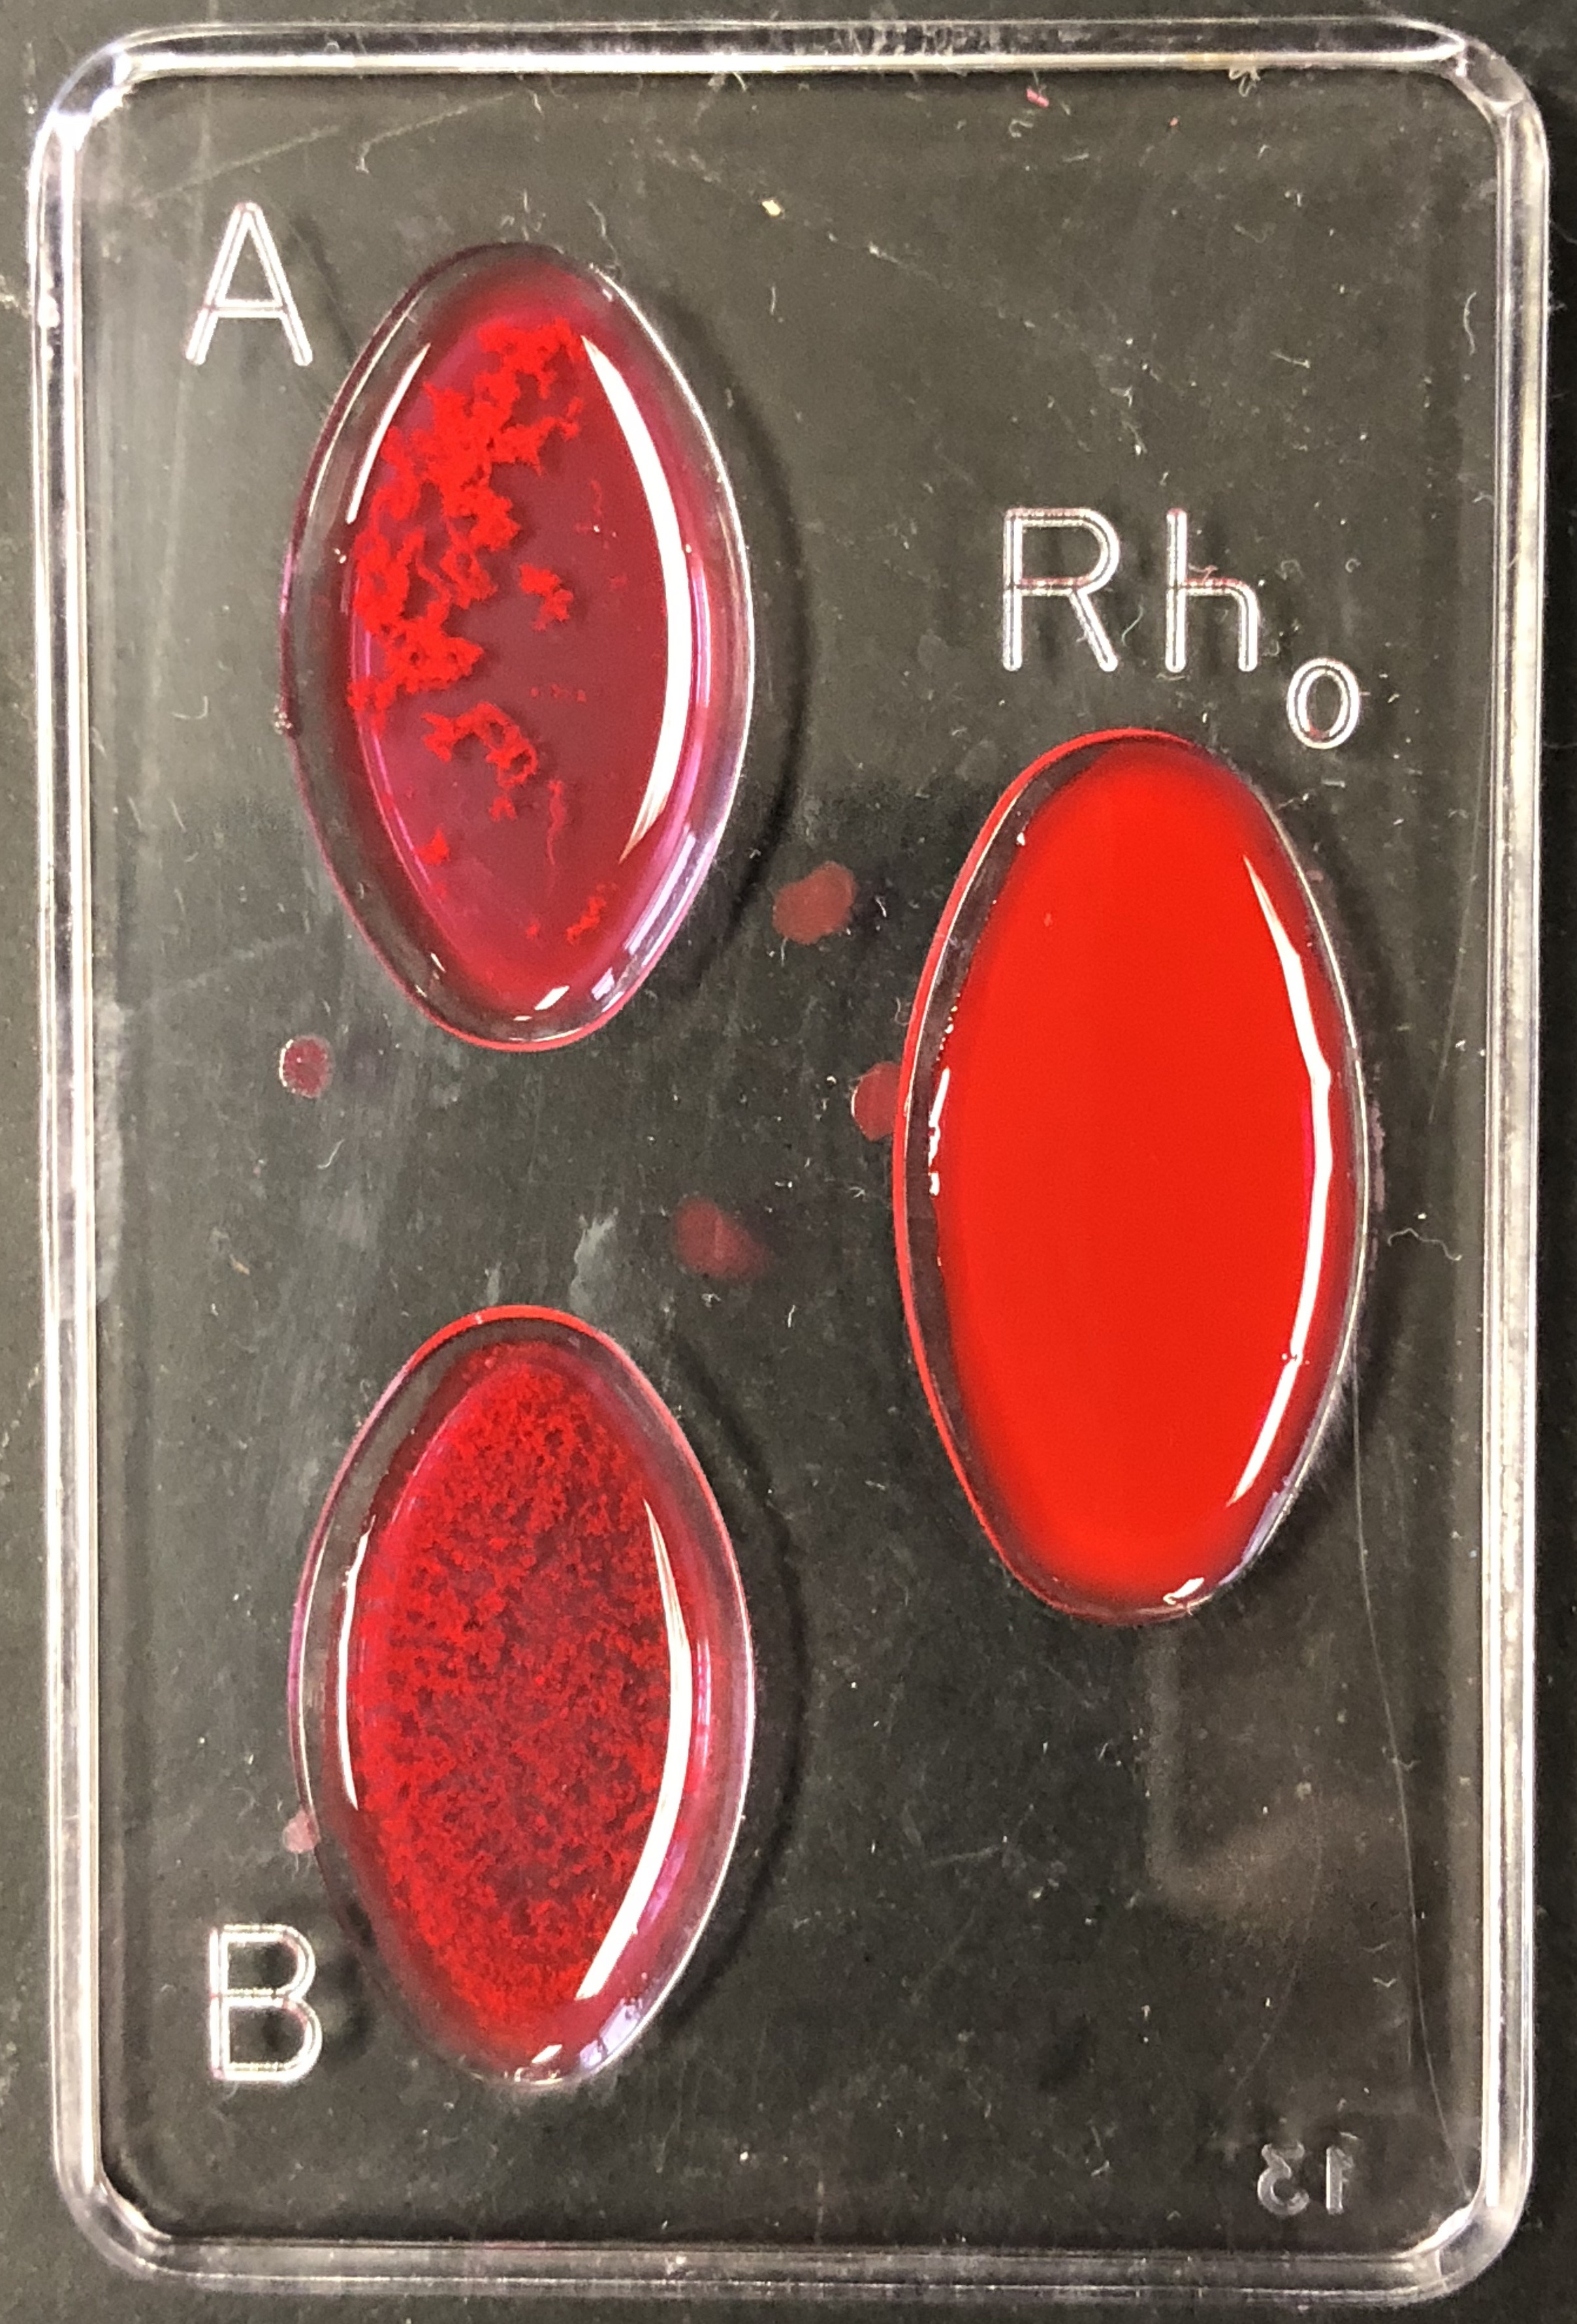
\includegraphics[width=0.7\linewidth]{./figures/mendel/blood_typing} 

}

\caption{Blood typing result}\label{fig:typing}
\end{figure}

\begin{longtable}[]{@{}lllll@{}}
\caption{\label{tab:blood} Blood Typing.}\tabularnewline
\toprule
& Sample 1 & Sample 2 & Sample 3 & Sample 4\tabularnewline
\midrule
\endfirsthead
\toprule
& Sample 1 & Sample 2 & Sample 3 & Sample 4\tabularnewline
\midrule
\endhead
Anti-A & & & &\tabularnewline
Anti-B & & & &\tabularnewline
Anti-D (Rh) + or - & & & &\tabularnewline
Blood Type & & & &\tabularnewline
\bottomrule
\end{longtable}

\section{Review Questions}\label{review-questions-7}

\begin{enumerate}
\def\labelenumi{\arabic{enumi}.}
\tightlist
\item
  What is a gene?
\item
  What is an allele?
\item
  What are dominant and recessive alleles?
\item
  What is the genotype of an organism?
\item
  What is a trait?
\item
  What is the phenotype of an organism?
\item
  What is the genotype of the F1 generation of the monohybrid cross?
\item
  What is the phenotype of the F1 generation monohybrid cross?
\item
  What are the possible maternal and paternal genotypes of the F1
  gametes monohybrid cross?
\item
  What is the genotype of the parents of the dihybrid cross?
\item
  What are the phenotypes of the parents of the dihybrid cross?
\item
  What are the possible genotypes of the parent gametes of the dihybrid
  cross?
\item
  What is the genotype of the F1 generation of the dihybrid cross?
\item
  What is the phenotype of the F1 generation dihybrid cross?
\item
  What are the possible maternal and paternal genotypes of the F1
  gametes dihybrid cross?
\end{enumerate}

\chapter{Molecular Biology}\label{molecular-biology}

\href{https://en.wikipedia.org/wiki/Molecular_biology}{Molecular
biology} concerns the molecular basis of biological activity between
biomolecules in the various systems of a cell, including the
interactions between DNA, RNA, and proteins and their biosynthesis, as
well as the regulation of these interactions.

One of the most basic techniques of molecular biology to study protein
function is molecular cloning. In this technique, DNA coding for a
protein of interest is cloned using polymerase chain reaction (PCR),
and/or restriction enzymes into a plasmid (expression vector). A vector
has 3 distinctive features: an origin of replication, a multiple cloning
site (MCS), and a selective marker usually antibiotic resistance.
Located upstream of the multiple cloning site are the promoter regions
and the transcription start site which regulate the expression of cloned
gene. This plasmid can be inserted into either bacterial or animal
cells. Introducing DNA into bacterial cells can be done by
transformation via uptake of naked DNA, conjugation via cell-cell
contact or by transduction via viral vector. Introducing DNA into
eukaryotic cells, such as animal cells, by physical or chemical means is
called transfection. Several different transfection techniques are
available, such as calcium phosphate transfection, electroporation,
microinjection and liposome transfection. The plasmid may be integrated
into the genome, resulting in a stable transfection, or may remain
independent of the genome, called transient transfection.

DNA coding for a protein of interest is now inside a cell, and the
protein can now be expressed. A variety of systems, such as inducible
promoters and specific cell-signaling factors, are available to help
express the protein of interest at high levels. Large quantities of a
protein can then be extracted from the bacterial or eukaryotic cell. The
protein can be tested for enzymatic activity under a variety of
situations, the protein may be crystallized so its tertiary structure
can be studied, or, in the pharmaceutical industry, the activity of new
drugs against the protein can be studied.

\section{DNA restriction digest}\label{dna-restriction-digest}

\href{https://en.wikipedia.org/wiki/Lambda_phage}{Lambda DNA} comes from
a virus
(\href{https://en.wikipedia.org/wiki/Bacteriophage}{bacteriophage}) that
infects bacteria. This virus does not infect humans and is therefore
safe source to work with. Lambda DNA is approximately 48,000 base pairs
long.

When restriction enzymes are used to cut DNA fragments of varying sizes
are produced. Cut DNA can be separated using a process known as
\href{https://en.wikipedia.org/wiki/Agarose_gel_electrophoresis}{agarose
gel electrophoresis}. Agarose gel electrophoresis separates DNA
fragments by molecular weight. DNA fragments are loaded into an agarose
gel slab, which is placed into a chamber filled with a conductive buffer
solution. A direct current is passed between positive (red) and negative
(black) wire electrodes at each end of the chamber. DNA fragments are
negatively charged, and when placed in an electric field will be drawn
toward the positive pole (red). The matrix of the agarose gel acts as a
molecular sieve through which smaller DNA fragments can move more easily
than larger ones. Therefore, the distance and rate at which DNA
fragments migrate through the gel is inversely proportional to its
molecular weight. Over a period of time smaller fragments will travel
farther than larger ones. Fragments of the same size stay together and
migrate in discrete ``bands''.

\section{Preparing a gel for agarose gel
electrophoresis}\label{preparing-a-gel-for-agarose-gel-electrophoresis}

We will use gel electrophoresis to separate the DNA fragments obtained
from the restriction digest (Figure \ref{fig:box}). Before setting up
the digest, we will pour agarose gel because it will take about half an
hour for the gel to harden.

\begin{figure}

{\centering 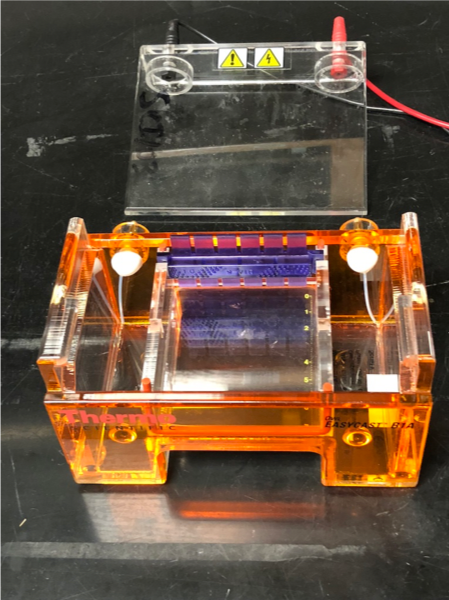
\includegraphics[width=0.7\linewidth]{./figures/molbio/Gel_box} 

}

\caption{Agarose gel box with comb in place, ready for gel to be poured.}\label{fig:box}
\end{figure}

\subsection{Experimental procedures}\label{experimental-procedures-32}

\begin{enumerate}
\def\labelenumi{\arabic{enumi}.}
\setcounter{enumi}{1}
\tightlist
\item
  Get the Erlenmeyer flask containing 0.5 g of agarose powder
\item
  Add 50 ml of 1x TAE (Tris base, acetic acid, EDTA) running buffer.
\item
  Add 5 µl of SybrGreen™ dye (10,000x stock solution).
\item
  Heat in the microwave at full power for 1 minute.
\item
  Swirl to make sure that all powder has dissolved, and the solution is
  clear.
\item
  Add the comb into the comb slot.
\item
  Pour the solution onto the gel tray in the gel box.
\end{enumerate}

\section{Setting up the restriction digest
reactions}\label{setting-up-the-restriction-digest-reactions}

In this experiment, we will use three
\href{https://en.wikipedia.org/wiki/Restriction_enzyme}{restriction
enzymes} (EcoRI, Hind III, and Pst I) to cut Lambda DNA.

\subsection{Experimental procedures}\label{experimental-procedures-33}

\begin{enumerate}
\def\labelenumi{\arabic{enumi}.}
\tightlist
\item
  Digest DNA: microtubes that contain the enzyme stock solution, Lambda
  DNA, and restriction buffer are provided on ice (in an ice bucket).
\item
  Get 4 new microtubes and label each as follows:

  \begin{itemize}
  \tightlist
  \item
    Tube 1: L = Lambda DNA
  \item
    Tube 2: P = Pst I digest
  \item
    Tube 3: E = EcoRI digest
  \item
    Tube4: H = Hind III digest
  \end{itemize}
\item
  Use a new pipette tip for each transfer and pipet the reagents (from
  the stock solutions kept on ice) into each tube according to Table
  \ref{tab:digest}.
\item
  Mix the components by gently flicking the tube with your finger. Pulse
  spin the tubes in the microcentrifuge to collect all the liquid to the
  bottom of the tube.
\item
  Place the tubes in the heat block and incubate for 30 minutes at 37
  °C.
\end{enumerate}

\begin{longtable}[]{@{}cccccc@{}}
\caption{\label{tab:digest} DNA digestion.}\tabularnewline
\toprule
Tube & DNA & buffer & Pst I & EcoR I & Hind III\tabularnewline
\midrule
\endfirsthead
\toprule
Tube & DNA & buffer & Pst I & EcoR I & Hind III\tabularnewline
\midrule
\endhead
L & 4 µl & 6 µl & \_ & \_ & \_\tabularnewline
P & 4 µl & 5 µl & 1 µl & \_ & \_\tabularnewline
E & 4 µl & 5 µl & \_ & 1 µl & \_\tabularnewline
H & 4 µl & 5 µl & \_ & \_ & 1 µl\tabularnewline
\bottomrule
\end{longtable}

\section{Loading the DNA samples on the agarose gel and agarose gel
electrophoresis}\label{loading-the-dna-samples-on-the-agarose-gel-and-agarose-gel-electrophoresis}

\begin{enumerate}
\def\labelenumi{\arabic{enumi}.}
\tightlist
\item
  Remove the digested DNA samples from the heat block.
\item
  Pulse spin the tubes in the centrifuge to bring all of the liquid to
  the bottom of the tube.
\item
  Add 2 µl of sample loading dye into each tube. Mix the contents by
  flicking the tube with your finger.
\item
  Fill the electrophoresis chamber and cover the gel with 1x TAE running
  buffer (this will require about 275 ml of buffer).
\item
  Check that the wells of the agarose gels are near the black (-)
  electrode and the base of the gel is near the red (+) electrode.
\item
  Load 12 µl of each sample into separate wells in the gel chamber in
  the following order:

  \begin{itemize}
  \tightlist
  \item
    Lane 1: L
  \item
    Lane 2: P
  \item
    Lane 3: E
  \item
    Lane 4: H
  \item
    Lane 5: DNA size marker
  \end{itemize}
\item
  Place the lid on the electrophoresis chamber. Connect the electrical
  leads into the power supply, red to red and black to black.
\item
  Turn on the power and run the gel at 120 V for 35 minutes (Figure
  \ref{fig:power}).
\end{enumerate}

\begin{figure}

{\centering 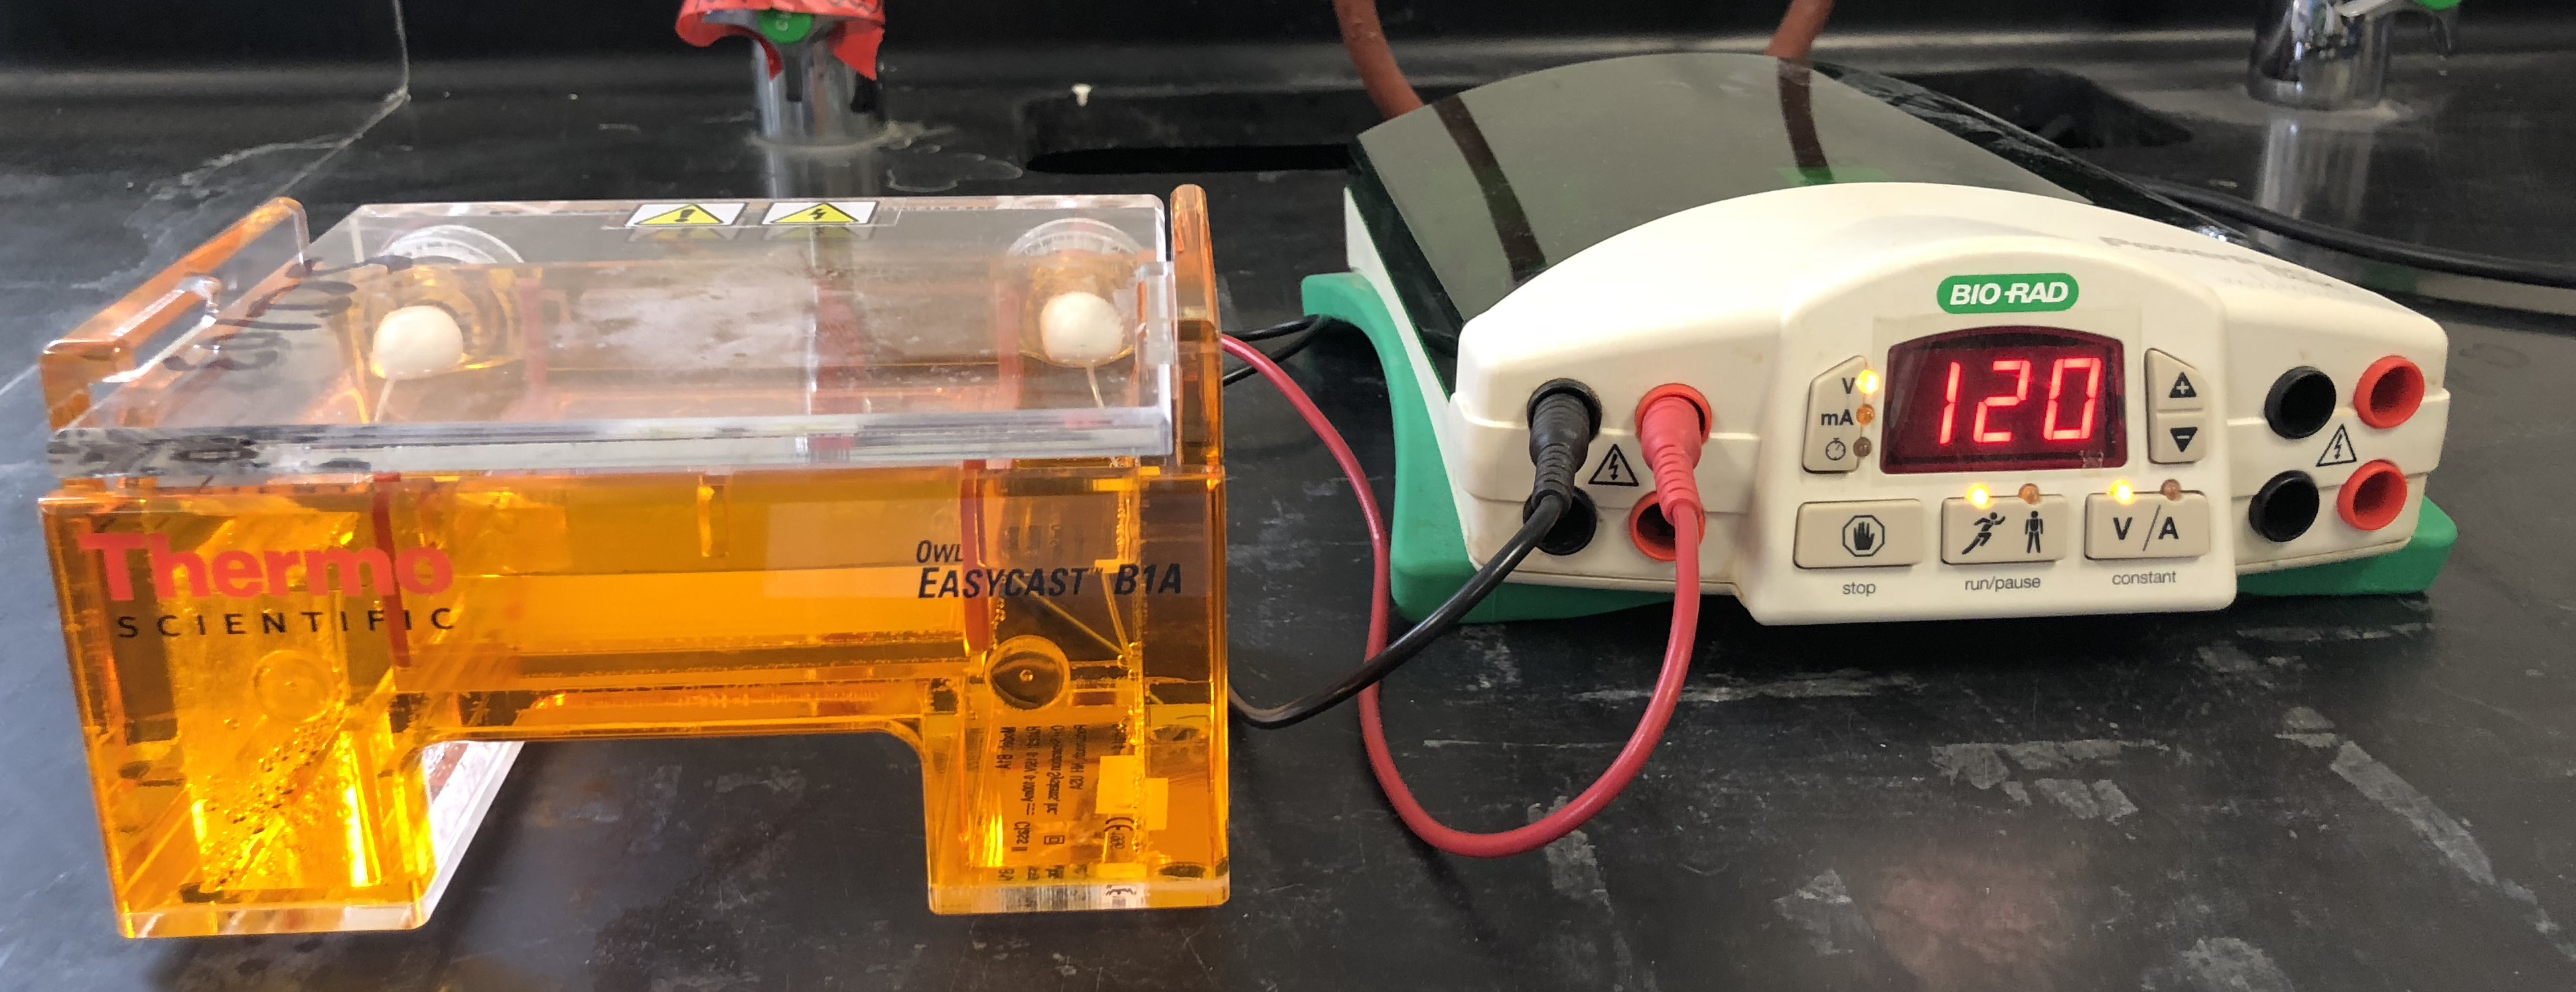
\includegraphics[width=0.7\linewidth]{./figures/molbio/Power_supply} 

}

\caption{Gel electrophoresis box and power supply.}\label{fig:power}
\end{figure}

\section{Visualizing the DNA fragments from the restriction
digest}\label{visualizing-the-dna-fragments-from-the-restriction-digest}

We added a non-toxic green fluorescent dye to the agarose before we
poured the gel. The inclusion of this dye will allow us to visualize the
separated DNA fragments by exposing the gel to UV light source in the UV
light box (Figure \ref{fig:doc}).

\subsection{Experimental procedures}\label{experimental-procedures-34}

\begin{enumerate}
\def\labelenumi{\arabic{enumi}.}
\tightlist
\item
  Visualize cut DNA using the UV light box (Figure \ref{fig:doc}).
\item
  Print out a picture of the gel.
\end{enumerate}

\begin{figure}

{\centering 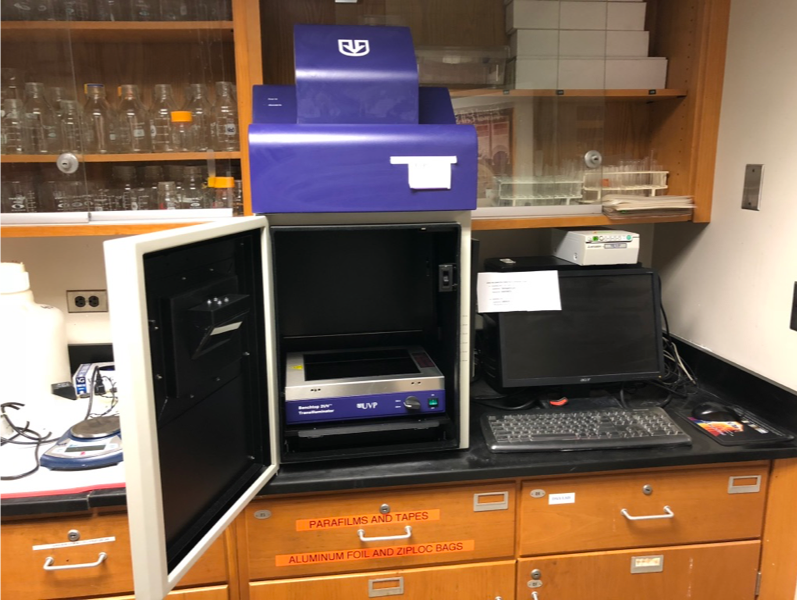
\includegraphics[width=0.7\linewidth]{./figures/molbio/Gel_doc} 

}

\caption{Gel documentation system with UV light source.}\label{fig:doc}
\end{figure}

\section{Review Questions}\label{review-questions-8}

\begin{enumerate}
\def\labelenumi{\arabic{enumi}.}
\tightlist
\item
  What is DNA made of?
\item
  What is a restriction enzyme?
\item
  What is a DNA ligase?
\item
  What is a DNA polymerase?
\item
  What is molecular cloning?
\item
  What is gel electrophoresis?
\item
  In an electric field, DNA moves from the \texttt{\_\_\_\_\_\_\_\_} to
  the \texttt{\_\_\_\_\_\_\_\_\_} pole.
\item
  Smaller fragments of DNA move \texttt{\_\_\_\_\_\_\_\_\_} than larger
  fragments.
\end{enumerate}

\chapter{Archaea and Bacteria}\label{archaea-and-bacteria}

In biological
\href{https://en.wikipedia.org/wiki/Taxonomy_(biology)}{taxonomy}, a
domain is the highest taxonomic rank of organisms in the
\href{https://en.wikipedia.org/wiki/Three-domain_system}{three-domain
system} of taxonomy designed by Carl Woese, an American microbiologist
and biophysicist. According to the Woese system, introduced in 1990, the
tree of life consists of three domains: Archaea, Bacteria, and Eukarya.
The first two are all prokaryotic microorganisms, or single-celled
organisms whose cells have no nucleus. All life that has a nucleus and
membrane-bound organelles, and multicellular organisms, is included in
the Eukarya.

\section{Bacteria}\label{bacteria}

\href{https://en.wikipedia.org/wiki/Bacteria}{Bacteria} (singular:
bacterium) are prokaryotic microorganisms. Typically, a few micrometers
in length, bacteria have a number of shapes, ranging from spheres to
rods and spirals. Bacteria were among the first life forms to appear on
Earth, and are present in most of its habitats. Bacteria inhabit soil,
water, acidic hot springs, radioactive waste, and the deep portions of
Earth's crust. Bacteria also live in symbiotic and parasitic
relationships with plants and animals. Most bacteria have not been
characterized, and only about half of the bacterial phyla have species
that can be grown in the laboratory. The study of bacteria is known as
bacteriology, a branch of microbiology. There are typically 40 million
bacterial cells in a gram of soil and a million bacterial cells in a
milliliter of fresh water. There are approximately
5x10\textsuperscript{30} bacteria on Earth forming a biomass which
exceeds that of all plants and animals. Bacteria are vital in many
stages of the nutrient cycle by recycling nutrients such as the fixation
of nitrogen from the atmosphere. The nutrient cycle includes the
decomposition of dead bodies and bacteria are responsible for the
putrefaction stage in this process. In the biological communities
surrounding hydrothermal vents and cold seeps, extremophile bacteria
provide the nutrients needed to sustain life by converting dissolved
compounds, such as hydrogen sulfide and methane, to energy. In March
2013, data reported by researchers in October 2012, was published. It
was suggested that bacteria thrive in the Mariana Trench, which with a
depth of up to 11 kilometers is the deepest known part of the oceans.
Other researchers reported related studies that microbes thrive inside
rocks up to 580 meters below the sea floor under 2.6 kilometers of ocean
off the coast of the northwestern United States. The largest number of
bacteria in humans exist in the gut flora, and a large number on the
skin. The vast majority of the bacteria in the body are rendered
harmless by the protective effects of the immune system, though many are
beneficial particularly in the gut flora. However, several species of
bacteria are pathogenic and cause infectious diseases. The most common
fatal bacterial diseases are respiratory infections, with tuberculosis
alone killing about 2 million people per year, mostly in sub-Saharan
Africa. In developed countries, antibiotics are used to treat bacterial
infections and are also used in farming, making antibiotic resistance a
growing problem. In industry, bacteria are important in sewage treatment
and the breakdown of oil spills, the production of cheese and yogurt
through fermentation, and the recovery of gold, palladium, copper and
other metals in the mining sector, as well as in biotechnology, and the
manufacture of antibiotics and other chemicals.

\section{Archaea}\label{archaea}

\href{https://en.wikipedia.org/wiki/Archaea}{Archaea} have unique
properties separating them from the other two domains of life, Bacteria
and Eukaryota. The Archaea are further divided into multiple recognized
phyla. Classification is difficult because the majority have not been
isolated in the laboratory and have only been detected by analysis of
their nucleic acids in samples from their environment. Archaea and
bacteria are generally similar in size and shape, although a few archaea
have very strange shapes. Despite this morphological similarity to
bacteria, archaea possess genes and several metabolic pathways that are
more closely related to those of eukaryotes, notably the enzymes
involved in transcription and translation. Other aspects of archaeal
biochemistry are unique, such as their reliance on ether lipids in their
cell membranes. Archaea use more energy sources than eukaryotes: these
range from organic compounds, such as sugars, to ammonia, metal ions or
even hydrogen gas. Salt-tolerant archaea use sunlight as an energy
source, and other species of archaea fix carbon; however, unlike plants
and cyanobacteria, no known species of archaea does both. Archaea
reproduce asexually by binary fission, fragmentation, or budding; unlike
bacteria and eukaryotes, no known species forms spores. Archaea were
initially viewed as extremophiles living in harsh environments, such as
hot springs and salt lakes, but they have since been found in a broad
range of habitats, including soils, oceans, and marshlands. They are
also part of the human microbiota, found in the colon, oral cavity, and
skin. Archaea are particularly numerous in the oceans, and the archaea
in plankton may be one of the most abundant groups of organisms on the
planet. Archaea are a major part of Earth's life and may play roles in
both the carbon cycle and the nitrogen cycle. No clear examples of
archaeal pathogens or parasites are known, but they are often mutualists
or commensals. One example is the methanogens that inhabit human and
ruminant guts, where their vast numbers aid digestion. Methanogens are
also used in biogas production and sewage treatment, and biotechnology
exploits enzymes from extremophile archaea that can endure high
temperatures and organic solvents.

\section{Eukarya}\label{eukarya}

Members of the domain Eukarya are called
\href{https://en.wikipedia.org/wiki/Eukaryote}{eukaryotes}. A eukaryote
is any organism whose cells have a cell nucleus and other organelles
enclosed within membranes) can be unicellular or multicellular
organisms. The defining feature that sets eukaryotic cells apart from
prokaryotic cells (Bacteria and Archaea) is that they have
membrane-bound organelles, especially the nucleus, which contains the
genetic material enclosed by the nuclear membrane. The presence of a
nucleus gives eukaryotes their name, which comes from the Greek eu,
``well'' or ``true'' and karyon, ``nut'' or ``kernel''. Eukaryotic cells
also contain other membrane-bound organelles such as mitochondria,
endoplasmic reticulum and the Golgi apparatus. In addition, plants and
algae contain chloroplasts. Unlike unicellular archaea and bacteria,
eukaryotes may also be multicellular and include organisms consisting of
many kinds of tissue and cell types. Eukaryotes can reproduce both
asexually through mitosis and sexually through meiosis and gamete
fusion. In mitosis, one cell divides to produce two genetically
identical cells. In meiosis, DNA replication is followed by two rounds
of cell division to produce four haploid daughter cells. These act as
sex cells (gametes). Each gamete has just one set of chromosomes, each a
unique mix of the corresponding pair of parental chromosomes resulting
from genetic recombination during meiosis. Eukaryotes evolved
approximately 1.6-2.1 billion years ago, during the Proterozoic eon.

\href{https://en.wikipedia.org/wiki/Virus}{Viruses} are not part of the
three-domain system.

\section{Gram stain}\label{gram-stain}

\href{https://en.wikipedia.org/wiki/Gram_stain}{Gram stain} or Gram
staining (Figure \ref{fig:gram}), also called Gram's method, is a method
of staining used to distinguish and classify bacterial species into two
large groups (gram-positive and gram-negative). The name comes from the
Danish bacteriologist Hans Christian Gram, who developed the technique.

\begin{figure}

{\centering 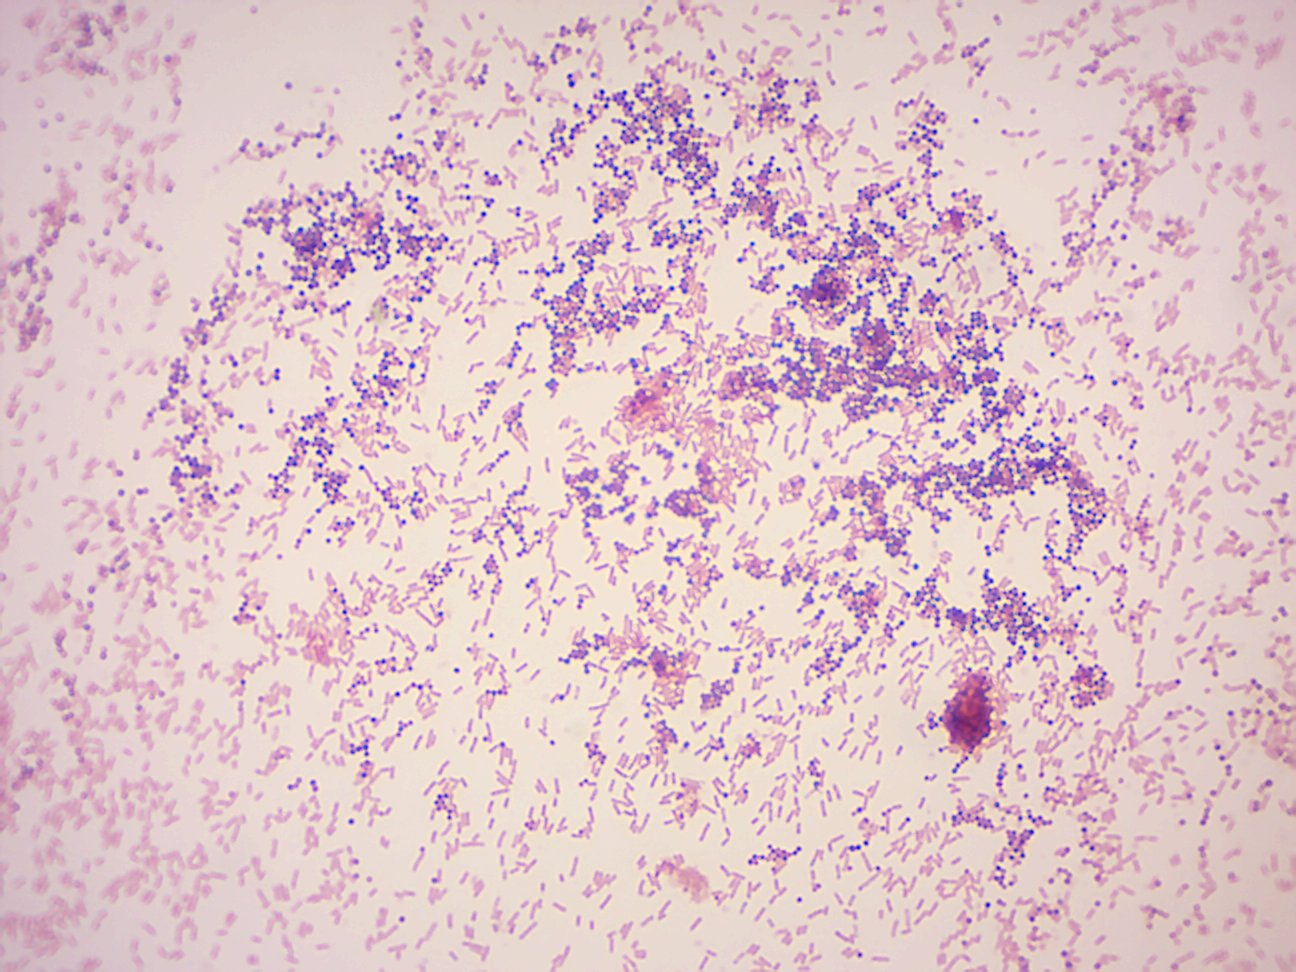
\includegraphics[width=0.7\linewidth]{./figures/bacteria/Gram_stain} 

}

\caption{Gram stained bacteria.}\label{fig:gram}
\end{figure}

Gram staining differentiates bacteria by the chemical and physical
properties of their cell walls by detecting peptidoglycan, which is
present in the cell wall of Gram-positive bacteria. Gram-negative cells
also contain peptidoglycan, but a very small layer of it that is
dissolved when the alcohol is added. This is why the cell loses its
initial color from the primary stain. Gram-positive bacteria retain the
crystal violet dye, and thus are stained violet, while the Gram-negative
bacteria do not; after washing, a counterstain is added (safranin) that
will stain these Gram-negative bacteria a pink color. Both Gram-positive
bacteria and Gram-negative bacteria pick up the counterstain. The
counterstain, however, is unseen on Gram-positive bacteria because of
the darker crystal violet stain.

\subsection{Experimental procedures}\label{experimental-procedures-35}

\begin{enumerate}
\def\labelenumi{\arabic{enumi}.}
\tightlist
\item
  Use a bacterial loop to pick up bacteria (Staphylococcus aureus and
  Escherichia coli) from the culture plate and streak out on a slide so
  that both samples partially overlap in the middle of the slide. Heat
  fix the sample to the slide by carefully passing the slide three times
  through a Bunsen burner flame.
\item
  Add crystal violet to the slide and incubate for 1 minute. Rinse slide
  with a gentle stream of water to remove unbound crystal violet.
\item
  Add Gram's iodine for 1 minute- this is the mordant, an agent that
  fixes the crystal violet to the bacterial cell wall.
\item
  Rinse slide with decolorizer until no more dye is running off. Rinse
  with a gentle stream of water.
\item
  Add safranin to the slide and incubate for 1 minute. Wash with a
  gentle stream of water. Gram positive bacteria it will retain crystal
  violet and stain purple. Gram negative will lose the primary stain and
  take the secondary stain causing it to appear pink when viewed under a
  microscope.
\item
  View under the microscope.
\end{enumerate}

\section{View living organisms}\label{view-living-organisms}

\subsection{Oscillatoria}\label{oscillatoria}

\href{https://en.wikipedia.org/wiki/Oscillatoria}{\emph{Oscillatoria}}
is a genus of filamentous cyanobacterium which is named after the
oscillation in its movement (Figure \ref{fig:oscillatoria}). Filaments
in the colonies can slide back and forth against each other until the
whole mass is reoriented to its light source. It is commonly found in
watering-troughs waters, and is mainly blue-green or brown-green.
Oscillatoria is an organism that reproduces by fragmentation.
Oscillatoria forms long filaments of cells which can break into
fragments called hormogonia. The hormogonia can grow into a new, longer
filament. Breaks in the filament usually occur where dead cells
(necridia) are present. Oscillatoria uses photosynthesis to survive and
reproduce. Each filament of oscillatoria consists of trichome which is
made up of rows of cells. The tip of the trichome oscillates like a
pendulum.

\begin{figure}

{\centering 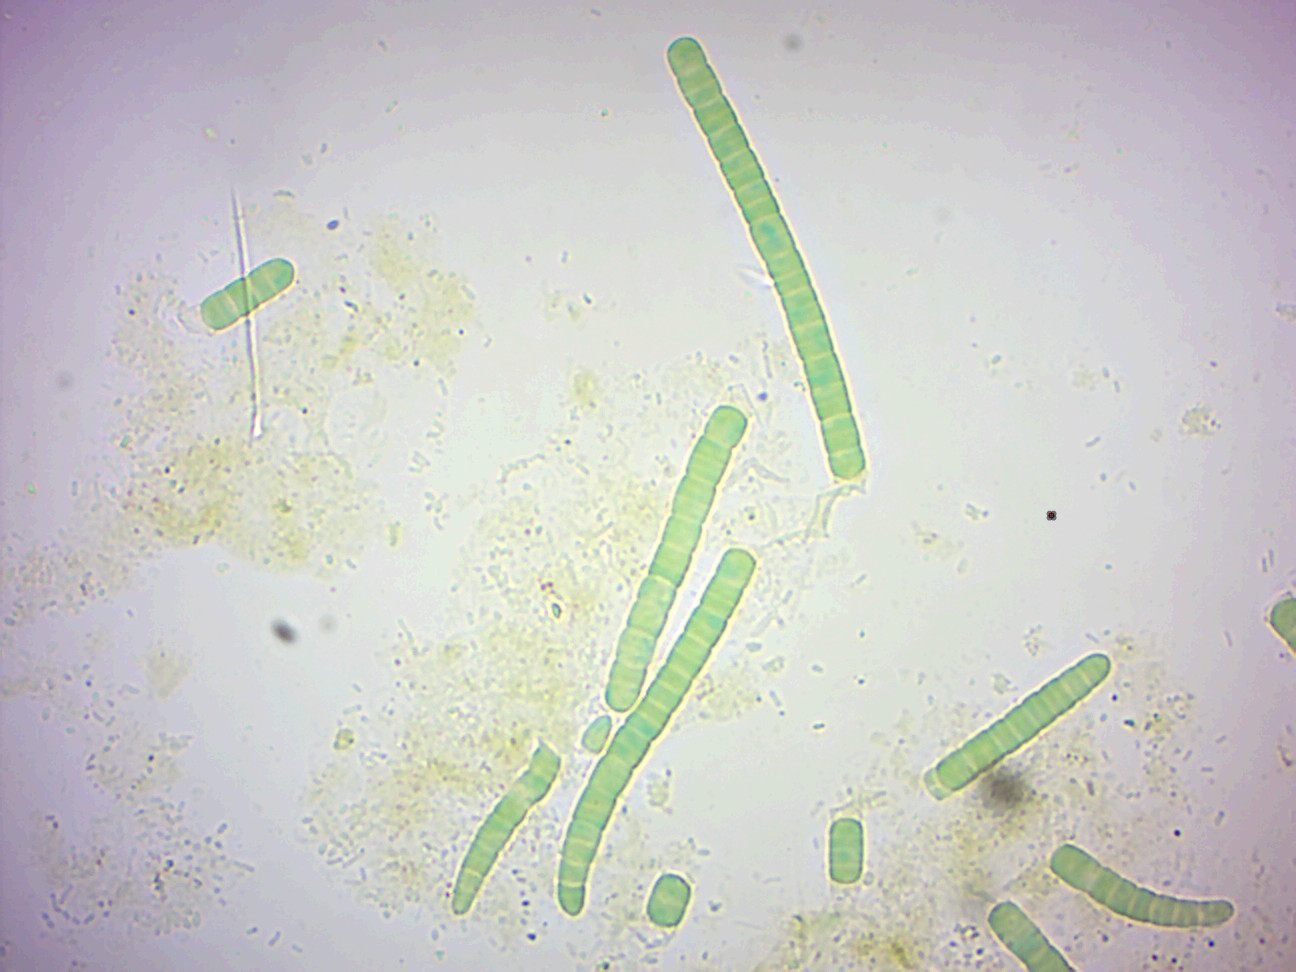
\includegraphics[width=0.7\linewidth]{./figures/bacteria/oscillatoria} 

}

\caption{Oscillatoria.}\label{fig:oscillatoria}
\end{figure}

\subsection{Nostoc}\label{nostoc}

\href{https://en.wikipedia.org/wiki/Nostoc}{\emph{Nostoc}} is a genus of
cyanobacteria found in various environments that forms colonies composed
of filaments of moniliform cells in a gelatinous sheath (Figure
\ref{fig:nostoc}). Nostoc can be found in soil, on moist rocks, at the
bottom of lakes and springs (both fresh- and saltwater), and rarely in
marine habitats. It may also grow symbiotically within the tissues of
plants, such as the evolutionarily ancient angiosperm Gunnera and the
hornworts (a group of bryophytes), providing nitrogen to its host
through the action of terminally differentiated cells known as
heterocysts. These bacteria contain photosynthetic pigments in their
cytoplasm to perform photosynthesis.

\begin{figure}

{\centering 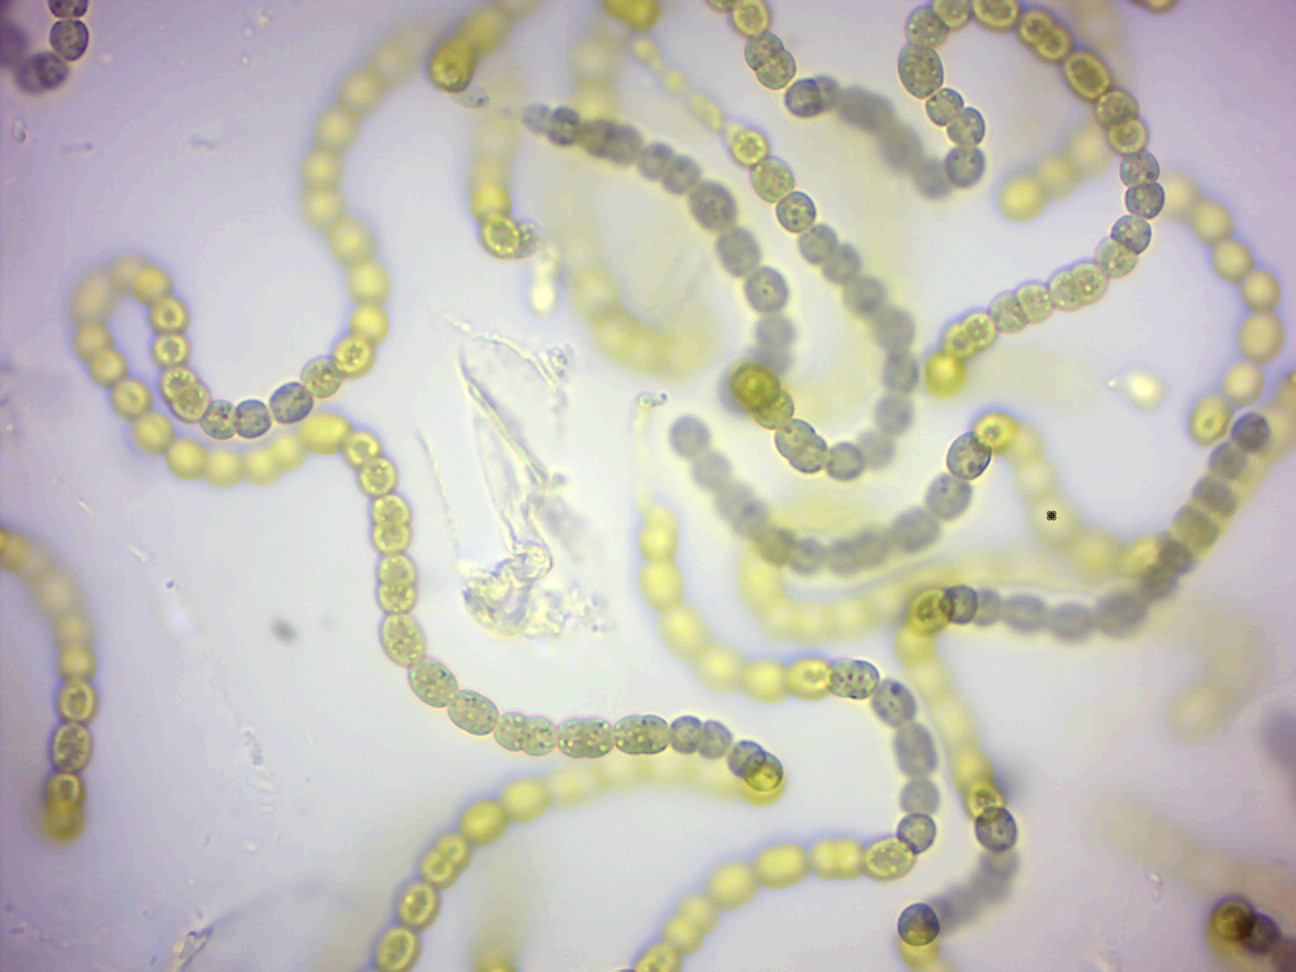
\includegraphics[width=0.7\linewidth]{./figures/bacteria/nostoc_live} 

}

\caption{Nostoc.}\label{fig:livenostoc}
\end{figure}

\subsection{Gloeocapsa}\label{gloeocapsa}

\href{https://en.wikipedia.org/wiki/Gloeocapsa}{\emph{Gloeocapsa}} (from
the Greek gloia (gelatinous) and the Latin capsa (case) is a genus of
cyanobacteria (Figure \ref{fig:gloeocapsa}). The cells secrete
individual gelatinous sheaths which can often be seen as sheaths around
recently divided cells within outer sheaths. Recently divided cell pairs
often appear to be only one cell since the new cells cohere temporarily.
They are also known as glow caps, a term derived from the yellowish hue
given off by the cap.

\begin{figure}

{\centering 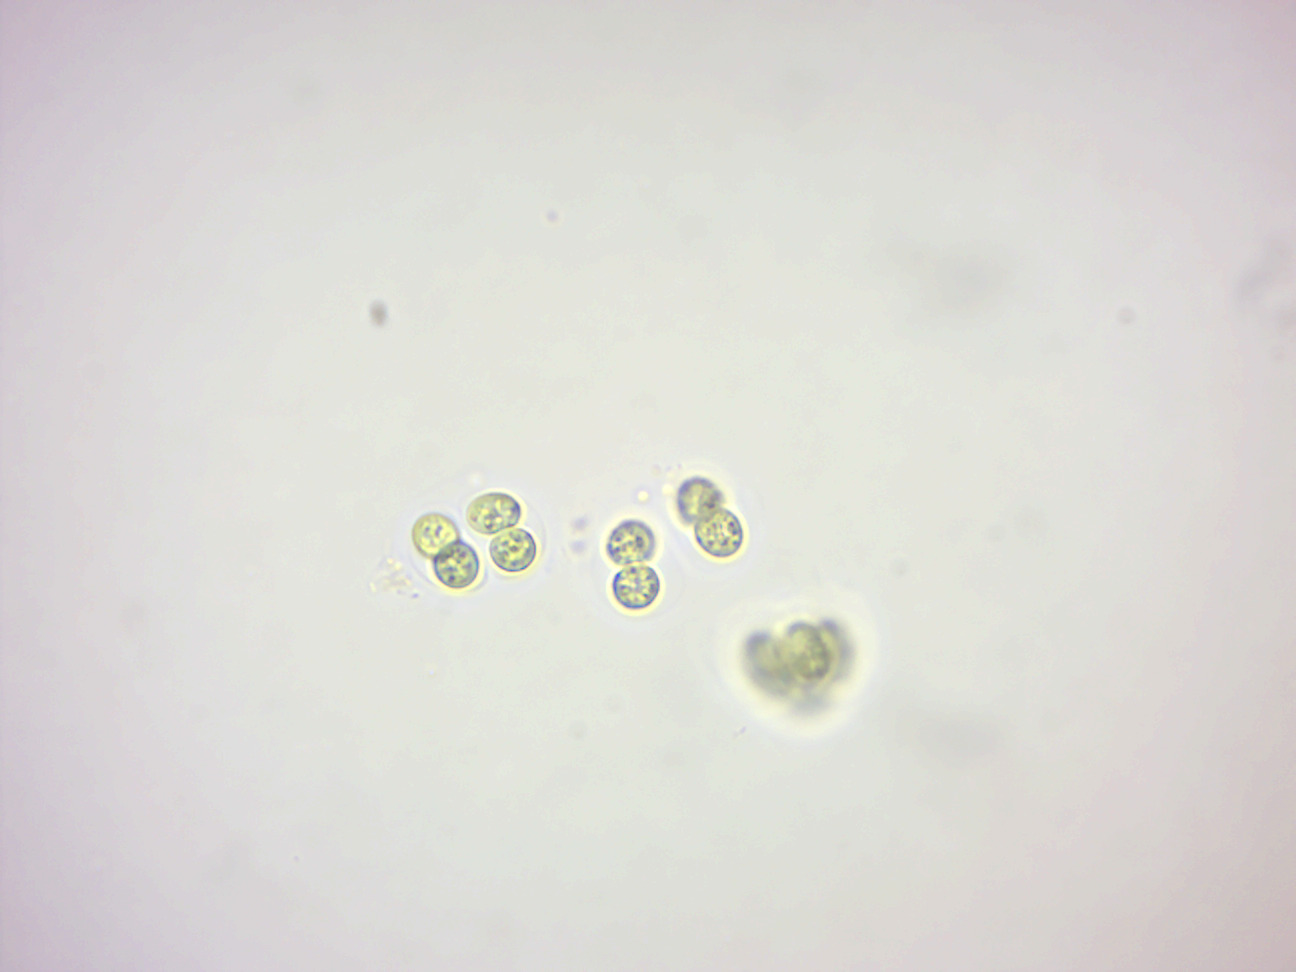
\includegraphics[width=0.7\linewidth]{./figures/bacteria/gloeocapsa} 

}

\caption{Gloeocapsa.}\label{fig:gloeocapsa}
\end{figure}

\section{View Prepared Slides}\label{view-prepared-slides-2}

\subsection{Mixed coccus (Gram stain) (Figure
\ref{fig:cocci}}\label{mixed-coccus-gram-stain-figure-reffigcocci}

\begin{figure}

{\centering 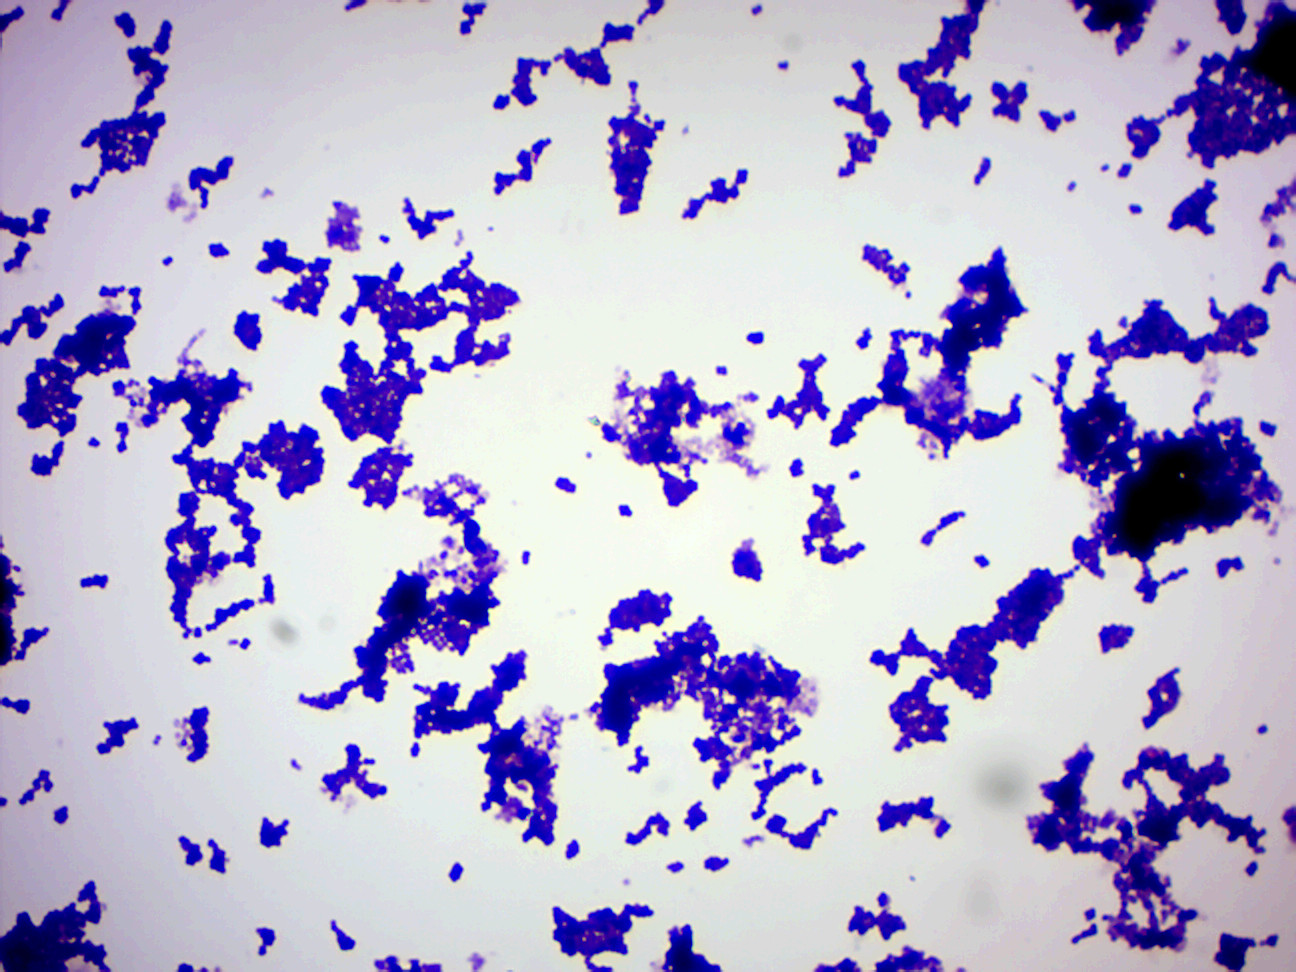
\includegraphics[width=0.7\linewidth]{./figures/bacteria/cocci} 

}

\caption{Mixed cocci.}\label{fig:cocci}
\end{figure}

\subsection{Mixed bacillus (Gram stain) (Figure
\ref{fig:bacilli}}\label{mixed-bacillus-gram-stain-figure-reffigbacilli}

\begin{figure}

{\centering 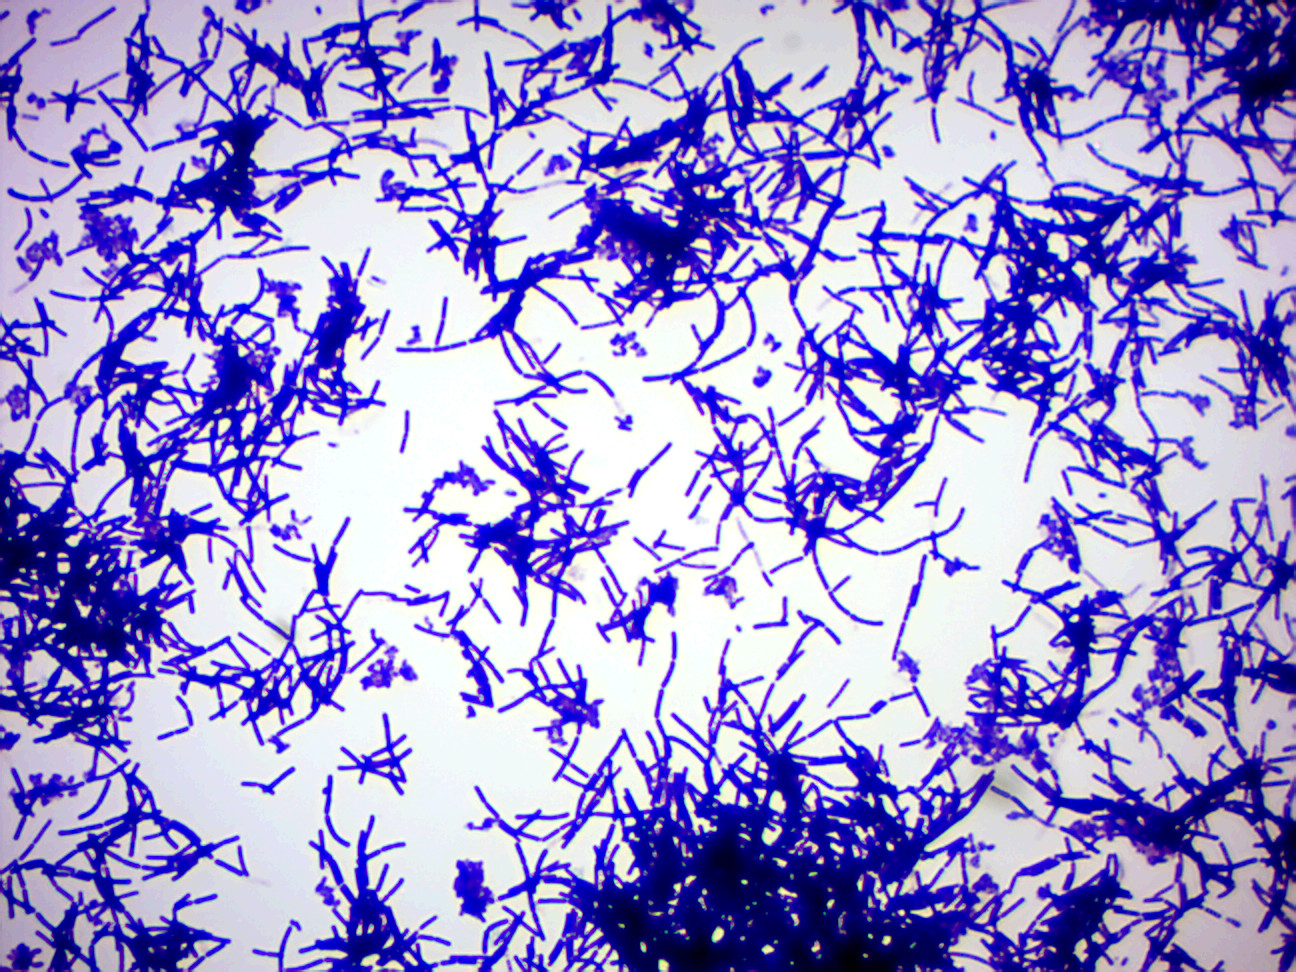
\includegraphics[width=0.7\linewidth]{./figures/bacteria/bacilli} 

}

\caption{Mixed bacilli.}\label{fig:bacilli}
\end{figure}

\subsection{Spirillum}\label{spirillum}

\href{https://en.wikipedia.org/wiki/Spirillum}{\emph{Spirillum}} is a
genus of Gram-negative bacteria (Figure \ref{fig:spirilla}). Members of
the genus Spirillum are large, elongate, spiral shaped, rigid cells.
Some have tufts of amphitrichous flagella at both poles. They are
microaerophilic and usually found in stagnant freshwater rich in organic
matter.

\begin{figure}

{\centering 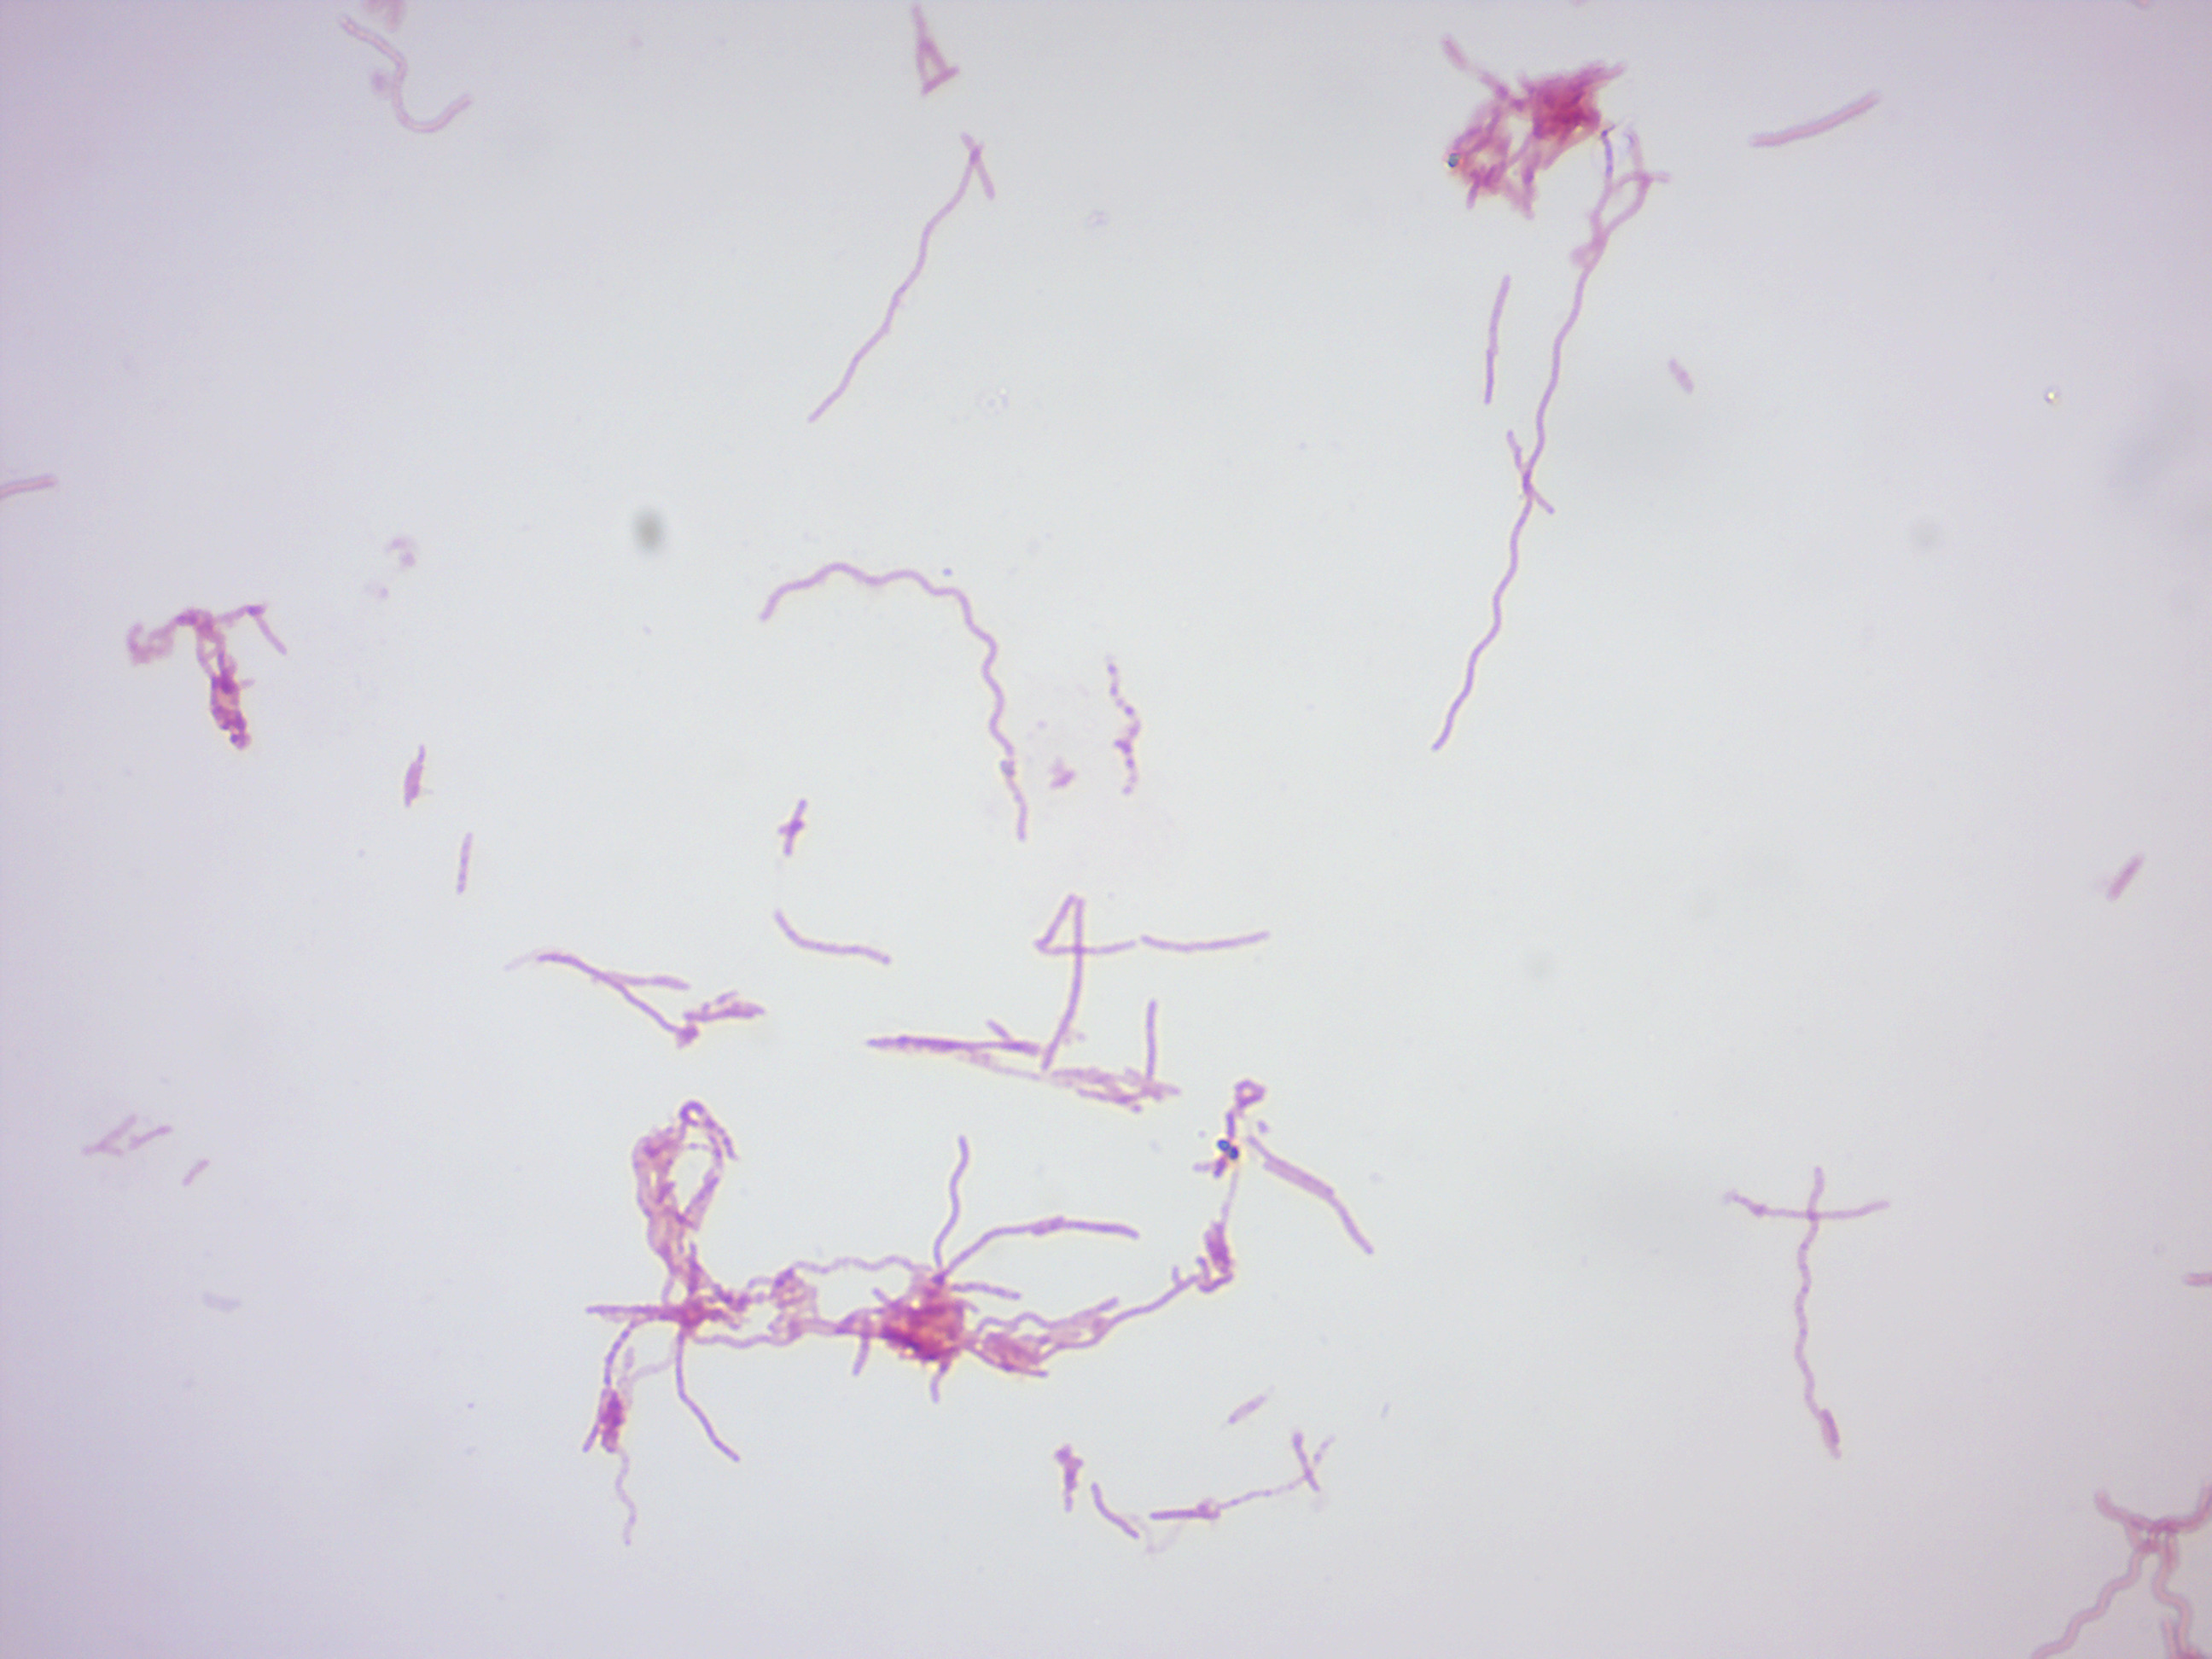
\includegraphics[width=0.7\linewidth]{./figures/bacteria/spirilla} 

}

\caption{Spirilla.}\label{fig:spirilla}
\end{figure}

\subsection{Treponema}\label{treponema}

\href{https://en.wikipedia.org/wiki/Treponema}{\emph{Treponema}} is a
genus of spiral-shaped Gram-negative bacteria (Figure
\ref{fig:treponema}). The major treponeme species of human pathogens is
Treponema pallidum, whose subspecies are responsible for diseases such
as syphilis, bejel, and yaws.

\begin{figure}

{\centering 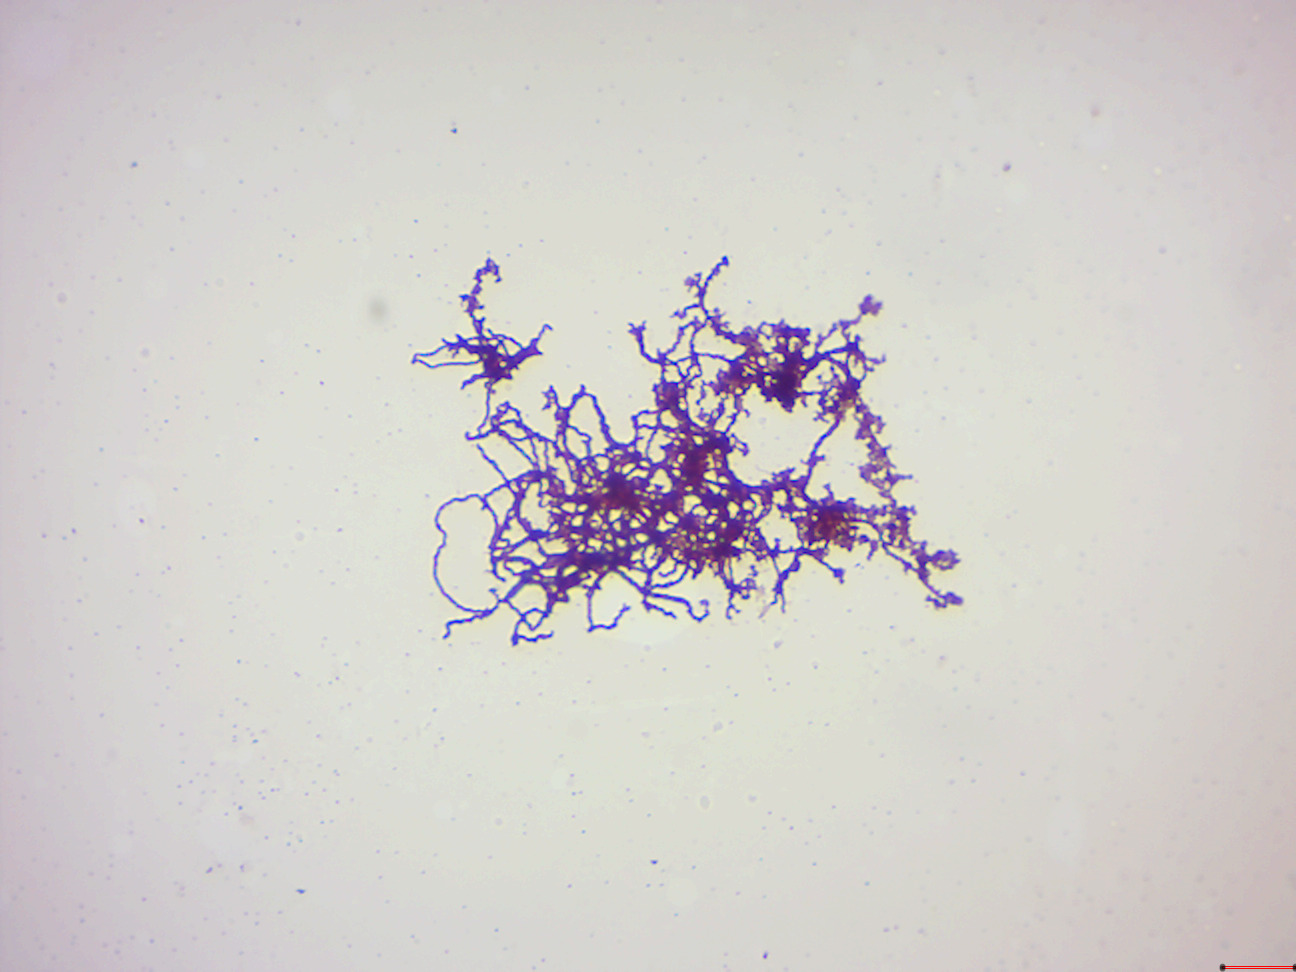
\includegraphics[width=0.7\linewidth]{./figures/bacteria/treponema} 

}

\caption{Treponema.}\label{fig:treponema}
\end{figure}

\subsection{Clostridium botulinum}\label{clostridium-botulinum}

\href{https://en.wikipedia.org/wiki/Clostridium_botulinum}{\emph{Clostridium
botulinum}} is a Gram-positive, rod-shaped, anaerobic, spore-forming,
motile bacterium with the ability to produce a neurotoxin known as
botulinum toxin. The botulinum toxin can cause a severe flaccid
paralytic disease in humans and other animals and is the most potent
toxin known to humankind, natural or synthetic, with a lethal dose of
1.3-2.1 ng/kg in humans. \emph{C. botulinum} is an obligate anaerobe,
meaning that oxygen is poisonous to the cells. However, it tolerates
traces of oxygen due to the enzyme superoxide dismutase, which is an
important antioxidant defense in nearly all cells exposed to oxygen. C.
botulinum is only able to produce the neurotoxin during sporulation,
which can only happen in an anaerobic environment. Other bacterial
species produce spores in an unfavorable growth environment to preserve
the organism's viability and permit survival in a dormant state until
the spores are exposed to favorable conditions.

\subsection{Staphylococcus aureus}\label{staphylococcus-aureus}

\href{https://en.wikipedia.org/wiki/Staphylococcus_aureus}{\emph{Staphylococcus
aureus}} (Figure \ref{fig:staph}) is a gram-positive, round-shaped
bacterium that is a member of the Firmicutes, and it is a member of the
normal flora of the body, frequently found in the nose, respiratory
tract, and on the skin. It is often positive for catalase and nitrate
reduction and is a facultative anaerobe that can grow without the need
for oxygen. Although S. aureus is not always pathogenic (and can
commonly be found existing as a commensal), it is a common cause of skin
infections including abscesses, respiratory infections such as
sinusitis, and food poisoning. Pathogenic strains often promote
infections by producing virulence factors such as potent protein toxins,
and the expression of a cell-surface protein that binds and inactivates
antibodies. The emergence of antibiotic-resistant strains of S. aureus
such as methicillin-resistant S. aureus (MRSA) is a worldwide problem in
clinical medicine.

\begin{figure}

{\centering 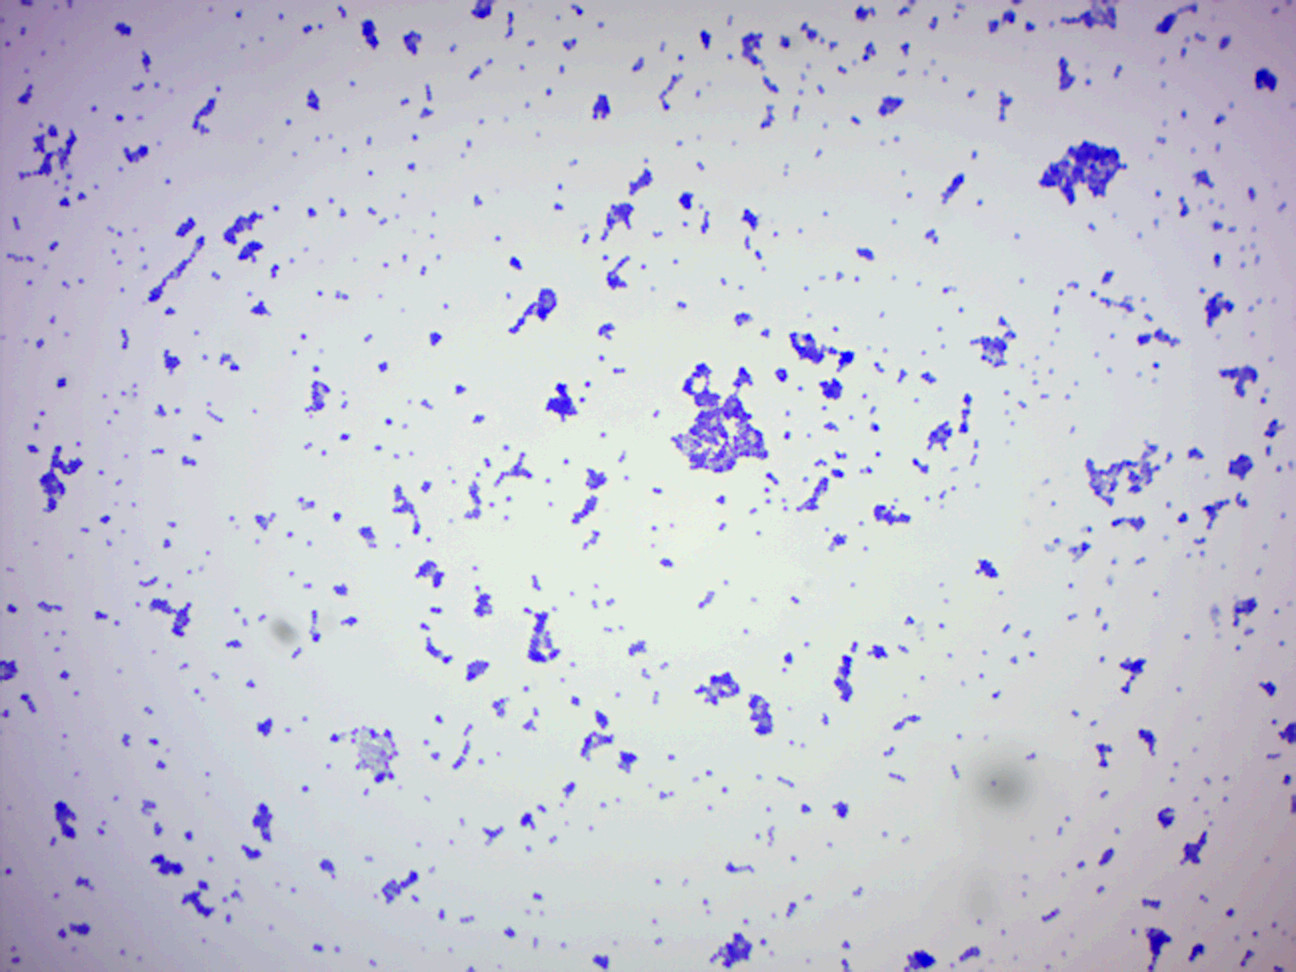
\includegraphics[width=0.7\linewidth]{./figures/bacteria/staphaureus} 

}

\caption{Staphylococcus aureus.}\label{fig:staph}
\end{figure}

\subsection{Oscillatoria}\label{oscillatoria-1}

\subsection{Nostoc (Figure
\ref{fig:nostoc})}\label{nostoc-figure-reffignostoc}

\begin{figure}

{\centering \includegraphics[width=0.7\linewidth]{./figures/bacteria/nostoc} 

}

\caption{Nostoc.}\label{fig:nostoc}
\end{figure}

\subsection{Anabaena}\label{anabaena}

\href{https://en.wikipedia.org/wiki/Anabaena}{\emph{Anabaena}} is a
genus of filamentous cyanobacteria that exist as plankton (Figure
\ref{fig:anabaena}). They are known for nitrogen-fixing abilities, and
they form symbiotic relationships with certain plants, such as the
mosquito fern. They are one of four genera of cyanobacteria that produce
neurotoxins, which are harmful to local wildlife, as well as farm
animals and pets. Production of these neurotoxins is assumed to be an
input into its symbiotic relationships, protecting the plant from
grazing pressure.

\begin{figure}

{\centering \includegraphics[width=0.7\linewidth]{./figures/bacteria/anabaena} 

}

\caption{Anabaena.}\label{fig:anabaena}
\end{figure}

\section{Review Questions}\label{review-questions-9}

\begin{enumerate}
\def\labelenumi{\arabic{enumi}.}
\tightlist
\item
  What are bacteria?
\item
  What are archaea?
\item
  What are eukarya?
\item
  What are cyanobacteria?
\end{enumerate}

\chapter{Protista}\label{protista}

\href{https://en.wikipedia.org/wiki/Protist}{Protists} are any
eukaryotic organism that are not an animal, plant or fungus. The
protists do not form a natural group, or clade, but are often grouped
together for convenience. In the popular five-kingdom scheme proposed by
Robert Whittaker in 1969, the protists make up a kingdom called
Protista, composed of ``organisms which are unicellular or
unicellular-colonial and which form no tissues. Some protists are
significant parasites of animals (e.g., five species of the parasitic
genus Plasmodium cause malaria in humans and many others cause similar
diseases in other vertebrates), plants (the oomycete Phytophthora
infestans causes late blight in potatoes) or even of other protists.
Protist pathogens share many metabolic pathways with their eukaryotic
hosts. This makes therapeutic target development extremely difficult - a
drug that harms a protist parasite is also likely to harm its
animal/plant host.

The term protista was first used by Ernst Haeckel in 1866. Protists were
traditionally subdivided into several groups based on similarities to
the ``higher'' kingdoms such as:

\begin{itemize}
\tightlist
\item
  \href{https://en.wikipedia.org/wiki/Protozoa}{Protozoa}: the
  unicellular ``animal-like'' (heterotrophic/parasitic) protozoa which
  were further sub-divided based on motility such as (flagellated)
  Flagellata, (ciliated) Ciliophora (or Ciliata), (phagocytic) amoeba
  and spore-forming Sporozoans
\item
  Protophyta: the ``plant-like'' (autotrophic) protophyta (mostly
  unicellular algae)
\item
  Molds: the ``fungus-like'' (saprophytic) slime molds and water molds.
\end{itemize}

The taxonomy of protists is ever changing. Newer classifications attempt
to present monophyletic groups based on morphological (especially
ultrastructural), biochemical (chemotaxonomy) and DNA sequence
(molecular research) information. However, there are sometimes
discordances between molecular and morphological investigations.

\section{View Living Organisms}\label{view-living-organisms-1}

\subsection{Amoeba proteus}\label{amoeba-proteus}

\href{https://en.wikipedia.org/wiki/Amoeba_proteus}{\emph{Amoeba
proteus}} (Figure \ref{fig:amoeba}) is an amoeba closely related to the
giant amoebae. This small protozoan uses tentacular protuberances called
pseudopodia to move and phagocytose smaller unicellular organisms,
(which may be greater in size than of amoeba), which are enveloped
inside the cell's cytoplasm in a food vacuole, where they are slowly
broken down by enzymes. It occupies freshwater environments and feeds on
other protozoans, algae, rotifers, and even other smaller amoebae. Due
to phytochromes, A. proteus may appear in a variety of colors (often
yellow, green and purple) under a microscope.

\begin{figure}

{\centering \includegraphics[width=0.7\linewidth]{./figures/protists/Amoeba_proteus} 

}

\caption{Amoeba proteus.}\label{fig:amoeba}
\end{figure}

\subsection{Paramecium caudatum}\label{paramecium-caudatum}

\href{https://en.wikipedia.org/wiki/Paramecium_caudatum}{\emph{Paramecium
caudatum}} (Figure \ref{fig:paramecium}) is a unicellular, ciliate
eukaryote. They can reach 0.25mm in length and are covered with minute
hair-like organelles called cilia. The cilia are used in locomotion and
feeding. P. caudatum feed on bacteria and small eukaryotic cells, such
as yeast and flagellate algae. In hypotonic conditions (freshwater), the
cell absorbs water by osmosis. It regulates osmotic pressure with the
help of bladder-like contractile vacuoles, gathering internal water
through its star-shaped radial canals and expelling the excess through
the plasma membrane. When moving through the water, they follow a spiral
path while rotating on the long axis. Paramecium have two nuclei (a
large macronucleus and a single compact micronucleus). They cannot
survive without the macronucleus and cannot reproduce without the
micro-nucleus. Like all ciliates, Paramecia reproduce asexually, by
binary fission. During reproduction, the macronucleus splits by a type
of amitosis, and the micronuclei undergo mitosis. The cell then divides
transversally, and each new cell obtains a copy of the micronucleus and
the macronucleus. Fission may occur as part of the normal vegetative
cell cycle. Under certain conditions, it may be preceded by
self-fertilization (autogamy), or it may follow conjugation, a sexual
phenomenon in which Paramecia of compatible mating types fuse
temporarily and exchange genetic material. During conjugation, the
micronuclei of each conjugant divide by meiosis and the haploid gametes
pass from one cell to the other. The gametes of each organism then fuse
to form diploid micronuclei. The old macronuclei are destroyed, and new
ones are developed from the new micronuclei. Without the rejuvenating
effects of autogamy or conjugation a Paramecium ages and dies. Only
opposite mating types, or genetically compatible organisms, can unite in
conjugation.

\begin{figure}

{\centering \includegraphics[width=0.7\linewidth]{./figures/protists/Paramecium_caudatum} 

}

\caption{Paramecium caudatum.}\label{fig:paramecium}
\end{figure}

\subsection{Euglena}\label{euglena}

\href{https://en.wikipedia.org/wiki/Euglena}{\emph{Euglena}} (Figure
\ref{fig:euglena}) is a genus of single-celled flagellate eukaryotes. It
is the best known and most widely studied member of the class
Euglenoidea, a diverse group containing some 54 genera and at least 800
species. Species of Euglena are found in fresh and salt waters. They are
often abundant in quiet inland waters where they may bloom in numbers
sufficient to color the surface of ponds and ditches green (E. viridis)
or red (E. sanguinea). When feeding as a heterotroph, Euglena takes in
nutrients by osmotrophy, and can survive without light on a diet of
organic matter, such as beef extract, peptone, acetate, ethanol or
carbohydrates. When there is sufficient sunlight for it to feed by
phototrophy, it uses chloroplasts containing the pigments chlorophyll a
and chlorophyll b to produce sugars by photosynthesis. Euglena's
chloroplasts are surrounded by three membranes, while those of plants
and the green algae (among which earlier taxonomists often placed
Euglena) have only two membranes. This fact has been taken as
morphological evidence that Euglena's chloroplasts evolved from a
eukaryotic green alga. Thus, the intriguing similarities between Euglena
and the plants would have arisen not because of kinship but because of a
secondary endosymbiosis. Molecular phylogenetic analysis has lent
support to this hypothesis, and it is now generally accepted.

\begin{figure}

{\centering \includegraphics[width=0.7\linewidth]{./figures/protists/euglena} 

}

\caption{Euglena.}\label{fig:euglena}
\end{figure}

\subsection{Peranema}\label{peranema}

\href{https://en.wikipedia.org/wiki/Peranema}{\emph{Peranema}} (Figure
\ref{fig:peranema}) is a genus of free-living flagellate, with more than
20 accepted species, varying in size between 8 and 200 micrometers. They
are found in freshwater lakes, ponds and ditches, and are often abundant
at the bottom of stagnant pools rich in decaying organic material.
Although they belong to the class Euglenoidea, and are morphologically
similar to the green Euglena, Peranema have no chloroplasts, and cannot
feed by autotrophy. Instead, they capture live prey, such as yeast,
bacteria and other flagellates, consuming them with the help of a rigid
feeding apparatus called a ``rod-organ.'' Unlike the green Euglenids,
they lack both an eyespot (stigma), and the paraflagellar body
(photoreceptor) that is normally coupled with that organelle. However,
while Peranema lack a localized photoreceptor, they do possess the
light-sensitive protein rhodopsin, and respond to changes in light with
a characteristic ``curling behavior.''

\begin{figure}

{\centering \includegraphics[width=0.7\linewidth]{./figures/protists/peranema} 

}

\caption{Peranema.}\label{fig:peranema}
\end{figure}

\subsection{Chlamydomonas}\label{chlamydomonas}

\href{https://en.wikipedia.org/wiki/Chlamydomonas}{\emph{Chlamydomonas}}
(Figure \ref{fig:chlamydomonaslive}) is a genus of green algae
consisting of unicellular flagellates, found in stagnant water and on
damp soil, in freshwater, seawater, and even in snow as ``snow algae''.
Chlamydomonas is used as a model organism for molecular biology,
especially studies of flagellar motility and chloroplast dynamics,
biogeneses, and genetics. One of the many striking features of
Chlamydomonas is that it contains ion channels, (channelrhodopsins),
that are directly activated by light. These proteins are used in
optogenetics.

\begin{figure}

{\centering \includegraphics[width=0.7\linewidth]{./figures/protists/chlamydomonas_live} 

}

\caption{Chlamydomonas. Note the flagella.}\label{fig:chlamydomonaslive}
\end{figure}

\subsection{Gymnodinium}\label{gymnodinium}

\href{https://en.wikipedia.org/wiki/Gymnodinium}{\emph{Gymnodinium}} is
a genus of
\href{https://en.wikipedia.org/wiki/Dinoflagellate}{dinoflagellates} It
is one of the few naked dinoflagellates, or species lacking armor
(cellulosic plates). The dinoflagellates (Greek dinos ``whirling'' and
Latin flagellum ``whip, scourge'') are a large group of flagellate
eukaryotes that constitute the phylum Dinoflagellata. Most are marine
plankton, but they are common in freshwater habitats, as well. Their
populations are distributed depending on temperature, salinity, or
depth. Many dinoflagellates are known to be photosynthetic, but a large
fraction of these are in fact mixotrophic, combining photosynthesis with
ingestion of prey (phagotrophy). In terms of number of species,
dinoflagellates form one of the largest groups of marine eukaryotes,
although this group is substantially smaller than the diatoms. Some
species are endosymbionts of marine animals and play an important part
in the biology of coral reefs. Other dinoflagellates are unpigmented
predators on other protozoa, and a few forms are parasitic.

\subsection{Pandorina}\label{pandorina}

\href{https://en.wikipedia.org/wiki/Pandorina}{\emph{Pandorina}} (Figure
\ref{fig:pandorina}) is a genus of green algae composed of 8, 16, or
sometimes 32 cells, held together at their bases to form a sack globular
colony surrounded by mucilage. The cells are ovoid or slightly narrowed
at one end to appear keystone- or pear-shaped. Each cell has two
flagella with two contractile vacuoles at their base, an eyespot, and a
large cup-shaped chloroplast with at least one pyrenoid. The colonies
co-ordinate their flagellar movement to create a rolling, swimming
motion. Pandorina shows the beginnings of the colony polarity and
differentiation seen in Volvox since the anterior cells have larger
eyespots. Asexual reproduction is by simultaneous division of all cells
of the colony to form autocolonies that are liberated by a
gelatinization of the colonial envelope. Sexual reproduction occurs by
division of each cell of the colony into 16-32 zoogametes. Zoogametes
show indications of heterogamy, a slight difference in the size and
motility of the pairs that fuse to form the smooth walled zygote.

\begin{figure}

{\centering \includegraphics[width=0.7\linewidth]{./figures/protists/Pandorina} 

}

\caption{Pandorina.}\label{fig:pandorina}
\end{figure}

\subsection{Volvox}\label{volvox}

\href{https://en.wikipedia.org/wiki/Volvox}{\emph{Volvox}} (Figure
\ref{fig:volvox}) is a genus of freshwater algae found in ponds and
ditches, even in shallow puddles. It forms spherical colonies of up to
50,000 cells that were first reported by Antonie van Leeuwenhoek in
1700. Volvox diverged from unicellular ancestors approximately 200
million years ago. Each mature Volvox colony is composed of up to
thousands of cells from two differentiated cell types: numerous
flagellate somatic cells and a smaller number of germ cells lacking in
soma that are embedded in the surface of a hollow sphere or coenobium
containing an extracellular matrix made of glycoproteins. Adult somatic
cells comprise a single layer with the flagella facing outward. The
cells swim in a coordinated fashion, with distinct anterior and
posterior poles. The cells have anterior eyespots that enable the colony
to swim towards light. An asexual colony includes both somatic
(vegetative) cells, which do not reproduce, and large, non-motile
gonidia in the interior, which produce new colonies through repeated
division. In sexual reproduction two types of gametes are produced.
Volvox species can be monoecious or dioecious. Male colonies release
numerous sperm packets, while in female colonies single cells enlarge to
become oogametes, or eggs. Volvox is facultatively sexual and can
reproduce both sexually and asexually. The switch from asexual to sexual
reproduction can be triggered by environmental conditions and by the
production of a sex-inducing pheremone. Desiccation-resistant diploid
zygotes are produced following successful fertilization.

\begin{figure}

{\centering \includegraphics[width=0.7\linewidth]{./figures/protists/Volvox} 

}

\caption{Volvox.}\label{fig:volvox}
\end{figure}

\subsection{Oedogonium}\label{oedogonium}

\href{https://en.wikipedia.org/wiki/Oedogonium}{\emph{Oedogonium}}
(Figure \ref{fig:oedogonium}) is a genus of filamentous green algae,
with unbranched filaments that are one cell thick. Oedogonium can be
free-floating, though it is usually attached to aquatic plants by a
holdfast. It appears greenish and inhabits calm, fresh water. Oedogonium
can reproduce asexually by fragmentation of the filaments, through some
other types of non-motile spores, and also through zoospores, which have
many flagella. These develop in a zoosporangium cell, one zoospore per
zoosporangium. After settling and losing its flagella, a zoospore grows
into a filament. Oedogonium can also reproduce sexually. Its sexual life
cycle is haplontic, i.e., the zygote undergoes meiosis. Antheridia
produce and release sperm, and oogonia produce and release an egg,. The
egg and sperm then fuse and form a zygote which is diploid (2n). The
zygote then undergoes meiosis to produce the filamentous green alga
which is haploid (1n).

\begin{figure}

{\centering \includegraphics[width=0.7\linewidth]{./figures/protists/oedogonium} 

}

\caption{Oedogonium.}\label{fig:oedogonium}
\end{figure}

\subsection{Spirogyra}\label{spirogyra}

\href{https://en.wikipedia.org/wiki/Spirogyra}{\emph{Spirogyra}} (Figure
\ref{fig:spiro}; common names include water silk, mermaid's tresses, and
blanket weed) is a genus of filamentous chlorophyte green algae of the
order Zygnematales, named for the helical or spiral arrangement of the
chloroplasts that is diagnostic of the genus. It is commonly found in
freshwater areas, and there are more than 400 species of Spirogyra in
the world. Spirogyra measures approximately 10 to 100 μm in width and
may grow to several centimeters in length. Spirogyra can reproduce both
sexually and asexually. In vegetative reproduction, fragmentation takes
place, and Spirogyra simply undergoes the intercalary mitosis to form
new filaments. Sexual Reproduction is of two types: 1. Scalariform
conjugation requires association of two different filaments lined side
by side either partially or throughout their length. One cell each from
opposite lined filaments emits tubular protuberances known as
conjugation tubes, which elongate and fuse, to make a passage called the
conjugation canal. The cytoplasm of the cell acting as the male travels
through this tube and fuses with the female cytoplasm, and the gametes
fuse to form a zygospore. 2. In lateral conjugation, gametes are formed
in a single filament. Two adjoining cells near the common transverse
wall give out protuberances known as conjugation tubes, which further
form the conjugation canal upon contact. The male cytoplasm migrates
through the conjugation canal, fusing with the female. The rest of the
process proceeds as in scalariform conjugation. The essential difference
is that scalariform conjugation occurs between two filaments and lateral
conjugation occurs between two adjacent cells on the same filament.

\begin{figure}

{\centering \includegraphics[width=0.7\linewidth]{./figures/protists/Spirogyra} 

}

\caption{Spirogyra.}\label{fig:spiro}
\end{figure}

\section{View Prepared Slides}\label{view-prepared-slides-3}

\subsection{Amoeba proteus}\label{amoeba-proteus-1}

\subsection{Paramecium 4 types of
protista}\label{paramecium-4-types-of-protista}

\subsection{Paramecium caudatum}\label{paramecium-caudatum-1}

\subsection{Paramecium in conjugation (Figure
\ref{fig:conjugation})}\label{paramecium-in-conjugation-figure-reffigconjugation}

\begin{figure}

{\centering \includegraphics[width=0.7\linewidth]{./figures/protists/paramecium_conjugation} 

}

\caption{Paramecium in conjugation.}\label{fig:conjugation}
\end{figure}

\subsection{Euglena}\label{euglena-1}

\subsection{Dinoflagellates}\label{dinoflagellates}

\subsection{Ceratium (Figure
\ref{fig:ceratium})}\label{ceratium-figure-reffigceratium}

\begin{figure}

{\centering \includegraphics[width=0.7\linewidth]{./figures/protists/ceratium} 

}

\caption{Ceratium, a dinoflagellate.}\label{fig:ceratium}
\end{figure}

\subsection{Peridinium
(dinoflagellate)}\label{peridinium-dinoflagellate}

\subsection{Foraminifera}\label{foraminifera}

\href{https://en.wikipedia.org/wiki/Foraminifera}{\emph{Foraminifera}}
(Figure \ref{fig:foraminifera}; Latin meaning hole bearers; informally
called ``forams'') are members of a phylum or class of amoeboid protists
characterized by: streaming granular ectoplasm for catching food and
other uses; and commonly an external shell (called a ``test'') of
diverse forms and materials. Most foraminifera are marine, the majority
of which live on or within the seafloor sediment (i.e., are benthic),
while a smaller variety float in the water column at various depths
(i.e., are planktonic). These shells are commonly made of calcium
carbonate (CaCO\textsubscript{3}) or agglutinated sediment particles.
Over 50,000 species are recognized, both living (10,000) and fossil
(40,000).

\begin{figure}

{\centering \includegraphics[width=0.7\linewidth]{./figures/protists/foraminifera} 

}

\caption{Foraminifera.}\label{fig:foraminifera}
\end{figure}

\subsection{Radiolaria}\label{radiolaria}

\href{https://en.wikipedia.org/wiki/Radiolaria}{\emph{Radiolaria}}
(Figure \ref{fig:radiolaria}), also called Radiozoa, are protozoa of
diameter 0.1-0.2 mm that produce intricate mineral skeletons, typically
with a central capsule dividing the cell into the inner and outer
portions of endoplasm and ectoplasm.The elaborate mineral skeleton is
usually made of silica. They are found as zooplankton throughout the
ocean, and their skeletal remains make up a large part of the cover of
the ocean floor as siliceous ooze.

\begin{figure}

{\centering \includegraphics[width=0.7\linewidth]{./figures/protists/radiolaria} 

}

\caption{Radiolaria.}\label{fig:radiolaria}
\end{figure}

\subsection{Diatoms}\label{diatoms}

\href{https://en.wikipedia.org/wiki/Diatom}{\emph{Diatoms}} (Figure
\ref{fig:diatomes}) are a major group of microalgae and are among the
most common types of phytoplankton. Diatoms are producers within the
food chain. A unique feature of diatom cells is that they are enclosed
within a cell wall made of silica (hydrated silicon dioxide) called a
frustule. These frustules show a wide diversity in form, but are usually
almost bilaterally symmetrical, hence the group name. These shells are
used by humans as diatomaceous earth, also known as diatomite. Fossil
evidence suggests that they originated during, or before, the early
Jurassic period. Only male gametes of centric diatoms are capable of
movement by means of flagella. Diatom communities are a popular tool for
monitoring environmental conditions, past and present, and are commonly
used in studies of water quality.

\begin{figure}

{\centering \includegraphics[width=0.7\linewidth]{./figures/protists/diatomes} 

}

\caption{Diatomes.}\label{fig:diatomes}
\end{figure}

\subsection{\texorpdfstring{\emph{Trypanosoma cruzi} and
\emph{Trypanosoma brucei
gambiense}}{Trypanosoma cruzi and Trypanosoma brucei gambiense}}\label{trypanosoma-cruzi-and-trypanosoma-brucei-gambiense}

\href{https://en.wikipedia.org/wiki/Trypanosoma_cruzi}{\emph{Trypanosoma
cruzi}} is a species of parasitic euglenoids. Amongst the protozoa, the
trypanosomes characteristically bore tissue in another organism and feed
on blood (primarily) and also lymph. This behaviour causes disease or
the likelihood of disease that varies with the organism: for example,
trypanosomiasis in humans (Chagas disease in South America). Parasites
need a host body and the haematophagous insect triatomine (descriptions
``assassin bug'', ``cone-nose bug'', and ``kissing bug'') is the major
vector in accord with a mechanism of infection. The triatomine likes the
nests of vertebrate animals for shelter, where it bites and sucks blood
for food. Individual triatomines infected with protozoa from other
contact with animals transmit trypanosomes when the triatomine deposits
its faeces on the host's skin surface and then bites. Penetration of the
infected faeces is further facilitated by the scratching of the bite
area by the human or animal host.

\href{https://en.wikipedia.org/wiki/Trypanosoma_brucei}{\emph{Trypanosoma
brucei}} (Figure \ref{fig:gambiense}) is a species of parasitic
kinetoplastid belonging to the genus Trypanosoma. The parasite is the
cause of a vector-borne disease of vertebrate animals, including humans,
carried by genera of tsetse fly in sub-Saharan Africa. In humans
\emph{T. brucei} causes African trypanosomiasis, or sleeping sickness.
In animals it causes animal trypanosomiasis, also called nagana in
cattle and horses. \emph{T. brucei} has traditionally been grouped into
three subspecies: \emph{T. b. brucei}, \emph{T. b. gambiense} and
\emph{T. b. rhodesiense}. The first is a parasite of non-human
vertebrates, while the latter two are the known parasites of humans.

\begin{figure}

{\centering \includegraphics[width=0.7\linewidth]{./figures/protists/gambiense} 

}

\caption{Trypanosoma brucei gambiense among red blood cells.}\label{fig:gambiense}
\end{figure}

\subsection{Plasmodium vivax}\label{plasmodium-vivax}

\href{https://en.wikipedia.org/wiki/Plasmodium_vivax}{\emph{Plasmodium
vivax}} is a protozoal parasite and a human pathogen. This parasite is
the most frequent and widely distributed cause of recurring (benign
tertian) malaria, P. vivax is one of the five species of malaria
parasites that commonly infect humans. Although it is less virulent than
Plasmodium falciparum, the deadliest of the five human malaria
parasites, P. vivax malaria infections can lead to severe disease and
death, often due to a pathologically enlarged spleen. P. vivax is
carried by the female Anopheles mosquito, since it is only the female of
the species that bites.

\subsection{Mixed green algae}\label{mixed-green-algae}

\subsection{Chlamydomonas (Figure
\ref{fig:chlamydomonas})}\label{chlamydomonas-figure-reffigchlamydomonas}

\begin{figure}

{\centering \includegraphics[width=0.7\linewidth]{./figures/protists/chlamydomonas} 

}

\caption{Chlamydomonas. Note the flagella.}\label{fig:chlamydomonas}
\end{figure}

\subsection{Pandorina (Figure
\ref{fig:pandorinadead})}\label{pandorina-figure-reffigpandorinadead}

\begin{figure}

{\centering \includegraphics[width=0.7\linewidth]{./figures/protists/pandorinadead} 

}

\caption{Pandorina.}\label{fig:pandorinadead}
\end{figure}

\subsection{Volvox (Figure
\ref{fig:volvoxdead})}\label{volvox-figure-reffigvolvoxdead}

\begin{figure}

{\centering \includegraphics[width=0.7\linewidth]{./figures/protists/volvox_dead} 

}

\caption{Volvox.}\label{fig:volvoxdead}
\end{figure}

\subsection{Volvox sexual stages (Figure
\ref{fig:volvoxsex})}\label{volvox-sexual-stages-figure-reffigvolvoxsex}

\begin{figure}

{\centering \includegraphics[width=0.7\linewidth]{./figures/protists/volvox_sex} 

}

\caption{Volvox sexual stages.}\label{fig:volvoxsex}
\end{figure}

\subsection{Spirogyra}\label{spirogyra-1}

\subsection{Oedogonium zygospores}\label{oedogonium-zygospores}

\subsection{Oedogonium macrandous}\label{oedogonium-macrandous}

\subsection{Fucus male and female
conceptacle}\label{fucus-male-and-female-conceptacle}

\href{https://en.wikipedia.org/wiki/Fucus}{\emph{Fucus}} is a genus of
brown algae found in the intertidal zones of rocky seashores almost
throughout the world. It has a relatively simple life cycle and produce
only one type of thallus which grows to a maximum size of 2 m. The
thallus is perennial with an irregular or disc-shaped holdfast or with
haptera. The erect portion of the thallus is dichotomous or subpinnately
branched, flattened and with a distinct midrib. Gas-filled pneumatocysts
(air-vesicles) are present in pairs in some species, one on either side
of the midrib. The gametangia develop in conceptacles embedded in
receptacles in the apices of the final branches. They may be monoecious
or dioecious. Fertile cavities, the conceptacles, containing the
reproductive cells are immersed in the receptacles near the ends of the
branches. After meiosis oogonia and antheridia are produced and
released, fertilisation follows and the zygote develops directly into
the diploid plant. It may be considered to be analogous to the life
cycle of the flowering plant, but in algae the oogonia are released and
fertilised in the sea while in flowering plants the ovules are
fertilised while attached to the parent plant and then released as a
seed.

\subsection{Fucus male conceptacle (Figure
\ref{fig:malefucus})}\label{fucus-male-conceptacle-figure-reffigmalefucus}

\begin{figure}

{\centering \includegraphics[width=0.7\linewidth]{./figures/protists/male_fucus} 

}

\caption{Fucus male conceptacle}\label{fig:malefucus}
\end{figure}

\subsection{Fucus female conceptacle (Figure
\ref{fig:femalefucus})}\label{fucus-female-conceptacle-figure-reffigfemalefucus}

\begin{figure}

{\centering \includegraphics[width=0.7\linewidth]{./figures/protists/female_fucus} 

}

\caption{Fucus female conceptacle}\label{fig:femalefucus}
\end{figure}

\subsection{\texorpdfstring{\emph{Polysiphonia}}{Polysiphonia}}\label{polysiphonia}

\href{https://en.wikipedia.org/wiki/Polysiphonia}{\emph{Polysiphonia}}
is a genus of filamentous red algae with about 19 species on the coasts
of the British Isles and about 200 species worldwide.

\subsection{\texorpdfstring{\emph{Stemonitis}}{Stemonitis}}\label{stemonitis}

\href{https://en.wikipedia.org/wiki/Stemonitis}{\emph{Stemonitis}}
(Figure \ref{fig:stemonitis}) is a distinctive genus of slime moulds
found throughout the world (except Antarctica). They are characterized
by the tall brown sporangia, supported on slender stalks, which grow in
clusters on rotting wood.

\begin{figure}

{\centering \includegraphics[width=0.7\linewidth]{./figures/protists/stemonitis} 

}

\caption{Stemonitis.}\label{fig:stemonitis}
\end{figure}

\subsection{\texorpdfstring{\emph{Saprolegnia}}{Saprolegnia}}\label{saprolegnia}

\href{https://en.wikipedia.org/wiki/Saprolegnia}{\emph{Saprolegnia}}
(Figure \ref{fig:saprolegnia}) is both a saprotroph and necrotroph.
Typically feeding on waste from fish or other dead cells, they will also
take advantage of creatures that have been injured. An infection is
known as oomycosis Saprolegnia is tolerant to a wide range of
temperature, 3 °C to 33 °C, but is more prevalent in lower temperatures.
While it is found most frequently in freshwater, it will also tolerate
brackish water and even moist soil. Saprolegnia filaments (hyphae) are
long with rounded ends, containing the zoospores. Saprolegnia generally
travels in colonies consisting of one or more species. They first form a
mass of individual hyphae. When the mass of hyphae grows large enough in
size to be seen without use of a microscope, it can be called a
mycelium.

\begin{figure}

{\centering \includegraphics[width=0.7\linewidth]{./figures/protists/saprolegnia} 

}

\caption{Saprolegnia.}\label{fig:saprolegnia}
\end{figure}

It has a diploid life cycle which includes both sexual and asexual
reproduction. In the asexual phase, a spore of Saprolegnia releases
zoospores. Within a few minutes, this zoospore will encyst, germinate
and release another zoospore. This second zoospore has a longer cycle
during which most dispersal happens; it will continue to encyst and
release a new spore in a process called polyplanetism until it finds a
suitable substrate. When a suitable medium is located, the hairs
surrounding the spore will lock onto the substrate so that the sexual
reproduction phase can start. It is also during this stage of
polyplanetism that the Saprolegnia are capable of causing infection; the
most pathogenic species have tiny hooks at the end of their hairs to
enhance their infectious ability. Once firmly attached, sexual
reproduction begins with the production of male and female gametangium,
antheridia and oogonium respectively. These unite and fuse together via
fertilization tubes. The zygote produced is named an oospore.

\section{Review Questions}\label{review-questions-10}

\begin{enumerate}
\def\labelenumi{\arabic{enumi}.}
\tightlist
\item
  What are protists?
\item
  What are ciliata?
\item
  What are flagellata?
\item
  How do amoeba move?
\item
  What are slime molds?
\end{enumerate}


\end{document}
